\documentclass[sigconf]{acmart}
% \settopmatter{authorsperrow=4}
%% \BibTeX command to typeset BibTeX logo in the docs
\AtBeginDocument{%
  \providecommand\BibTeX{{%
    \normalfont B\kern-0.5em{\scshape i\kern-0.25em b}\kern-0.8em\TeX}}}

\usepackage{graphicx}

% \usepackage{amsfonts}

\usepackage{booktabs}
\usepackage{multirow}
\usepackage{enumitem}
\usepackage{physics,amsmath}
\let\Bbbk\relax 
\usepackage{amssymb}
% \usepackage{unicode-math}
% \usepackage{amsmath}
\usepackage{colortbl}
% \usepackage{bm}
\newcommand{\wx}[1]{{\color{black}{#1}}}
\newcommand{\za}[1]{{\color{black}{#1}}}
\newcommand{\lyc}[1]{{\color{black}{#1}}}
\newcommand{\imp}[1]{{\color{red}{#1}}}
\newcommand{\white}[1]{{\color{white}{#1}}}
\definecolor{gray}{rgb}{ 0.851,  0.851,  0.851}

\newcommand{\ie}{\emph{i.e., }}
\newcommand{\eg}{\emph{e.g., }}
\newcommand{\etal}{\emph{et al. }}
\newcommand{\st}{\emph{s.t. }}
\newcommand{\etc}{\emph{etc.}}
\newcommand{\wrt}{\emph{w.r.t. }}
\newcommand{\cf}{\emph{cf. }}
\newcommand{\aka}{\emph{a.k.a. }}

\newcommand*\rot{\rotatebox{90}}

\copyrightyear{2022}
\acmYear{2022}
\setcopyright{rightsretained}
\acmConference[MM '22]{Proceedings of the 30th ACM International Conference on Multimedia}{October 10--14, 2022}{Lisboa, Portugal}
\acmBooktitle{Proceedings of the 30th ACM International Conference on Multimedia (MM '22), Oct. 10--14, 2022, Lisboa, Portugal}
\acmDOI{10.1145/3503161.3548035}
\acmISBN{978-1-4503-9203-7/22/10}
\acmPrice{15.00}

% Overwrite copyright field outside from cls file.
\usepackage{etoolbox}
\makeatletter
\patchcmd{\maketitle}{\@copyrightpermission}{
   \begin{minipage}{0.3\columnwidth}
     \href{https://creativecommons.org/licenses/by/4.0/}{
\includegraphics[width=0.90\textwidth]{fig/cc_by4acm.png}}
   \end{minipage}\hfill
   \begin{minipage}{0.7\columnwidth}
     \href{https://creativecommons.org/licenses/by/4.0/}{This work is licensed under a Creative Commons Attribution International 4.0 License.}
   \end{minipage}

   \vspace{5pt}
}{}{}

\makeatother

% \author{Yicong Li}
% \email{liyicong@u.nus.edu.sg}
% \affiliation{%
%   \institution{National University of Singapore}
%     \country{}}

% \author{Xiang Wang}
% \authornote{Corresponding author. This research is supported by the Sea-NExT Joint Lab, and the CCCD Key Lab of Ministry of Culture and Tourism, USTC.}
% \email{xiangwang1223@gmail.com}
% \affiliation{%
%   \institution{University of Science and Technology of China}    
%   \country{}}

% \author{Junbin Xiao}
% \email{junbin@comp.nus.edu.sg}
% \affiliation{%
%   \institution{National University of Singapore}
%       \country{}}

% \author{Tat-Seng Chua}
% \email{dcscts@nus.edu.sg}
% \affiliation{%
%   \institution{National University of Singapore}
%       \country{}}


\author{Yicong Li$^{1}$, Xiang Wang$^{2*}$, Junbin Xiao$^{1}$, and Tat-Seng Chua$^1$}
\def\authors{Yicong Li, Xiang Wang, Junbin Xiao, and Tat-Seng Chua}
\affiliation{
\institution{$^1$National University of Singapore, $^2$University of Science and Technology of China}
\country{}
}
\email{liyicong@u.nus.edu, xiangwang1223@gmail.com, junbin@comp.nus.edu.sg, dcscts@nus.edu.sg}
\thanks{$*$ Corresponding author. This research is supported by the Sea-NExT Joint Lab, and the CCCD Key Lab of Ministry of Culture and Tourism, USTC.}
     
\renewcommand{\shortauthors}{Li et al.}


\begin{document}
% \settopmatter{printacmref=false}

\title{Equivariant and Invariant Grounding for Video Question Answering}

\begin{abstract}
Video Question Answering (VideoQA) is the task of answering the natural language questions about a video.
Producing an answer requires understanding the interplay across visual scenes in video and linguistic semantics in question.
However, most leading VideoQA models work as black boxes, which make the visual-linguistic alignment behind the answering process obscure.
Such black-box nature calls for visual explainability that reveals ``What part of the video should the model look at to answer the question?''.
Only a few works present the visual explanations in a post-hoc fashion, which emulates the target model's answering process via an additional method.
% , such as visualizing the attention or gradient-like scores of visual scenes.
Nonetheless, the emulation struggles to faithfully exhibit the visual-linguistic alignment during answering.

Instead of post-hoc explainability, we focus on intrinsic interpretability to make the answering process transparent.
At its core is grounding the question-critical cues as the causal scene to yield answers, while rolling out the question-irrelevant information as the environment scene.
Taking a causal look at VideoQA,
we devise a self-interpretable framework, \underline{E}quivariant and \underline{I}nvariant \underline{G}rounding for Interpretable \underline{V}ideoQA (EIGV).
Specifically, the equivariant grounding encourages the answering to be sensitive to the semantic changes in the causal scene and question; in contrast, the invariant grounding enforces the answering to be insensitive to the changes in the environment scene.
By imposing them on the answering process, EIGV is able to distinguish the causal scene from the environment information, and explicitly present the visual-linguistic alignment.
Extensive experiments on three benchmark datasets justify the superiority of EIGV in terms of accuracy and visual interpretability over the leading baselines.
Our code is available at \url{https://github.com/yl3800/EIGV}.

\end{abstract}

%%
%% The code below is generated by the tool at http://dl.acm.org/ccs.cfm.
%% Please copy and paste the code instead of the example below.
%%

\begin{CCSXML}
<ccs2012>
   <concept>
       <concept_id>10002951.10003317.10003347.10003348</concept_id>
       <concept_desc>Information systems~Question answering</concept_desc>
       <concept_significance>500</concept_significance>
       </concept>
   <concept>
       <concept_id>10002951.10003317.10003371.10003386</concept_id>
       <concept_desc>Information systems~Multimedia and multimodal retrieval</concept_desc>
       <concept_significance>500</concept_significance>
       </concept>
 </ccs2012>
\end{CCSXML}

\ccsdesc[500]{Information systems~Question answering}
\ccsdesc[500]{Information systems~Multimedia and multimodal retrieval}

%%
%% Keywords. The author(s) should pick words that accurately describe
%% the work being presented. Separate the keywords with commas.
\keywords{\lyc{Video Question Answering, Invariant Learning, Equivariant Learning, Interpretability}}

\maketitle
\begin{sloppypar}

\section{Introduction}
\label{sec:introduction}

\begin{figure}[t]
\centering
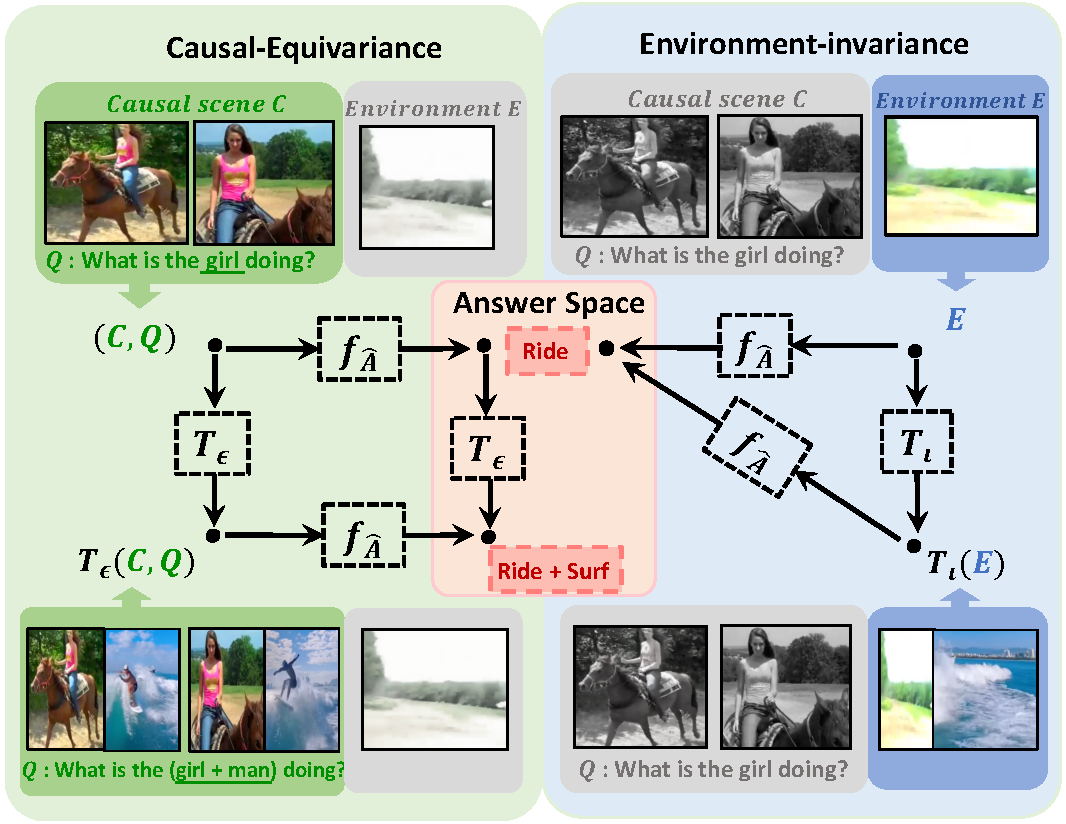
\includegraphics[scale=0.47]{fig/f1.pdf}
\vspace{-15pt}
\caption{
Illustration of equivariant and invariant grounding.
The causal-equivariant principle (left) asks that the semantic change $T_{\epsilon}$ applied to the causal scene $C$ and question $Q$ should be faithfully reflected in the answer change.
In contrast, the environment-invariant principle (right) outputs the same answer, regardless of changes $T_{\iota}$ on the environment scene $E$.
Here, $f_{\hat{A}}$ maps input to answer space.
}
\vspace{-15pt}
\label{fig:overview}
\end{figure}

% 1.videoQA overview-----------------------------------------
Video Question Answering (VideoQA) \cite{zhong2022video} is a keystone in interactive AI, such as vision-language navigation and communication systems.
It aims to answer the natural language question based on the video content.
Striving for the architecture novelty, many studies have been conducted on modeling VideoQA's multi-modal nature, such as fostering the vision-language alignment \cite{jiang2020reasoning,park2021bridge} and revisiting the visual input structure \cite{le2021hierarchical,dang2021hierarchical}.
However, existing VideoQA models usually operate as black boxes, which fail to exhibit the working mechanism behind the predictions and hardly exhibit ``What knowledge should the model use to answer the question about the video?''.
As a result, the black-box nature causes concern for the model's reliability, especially in applications to safety and security.



% 2.problem of interpretable-------------------------------
The concern on the black-box nature calls for  \lyc{better transparency} of VideoQA models.
Here we focus on visual-explainability \cite{CSS,DBLP:conf/ijcai/RossHD17}, aiming to reveal ``Which part of the video should the model look at to answer the question?''.
It requires us to find a subset of visual scenes --- rationale --- \lyc{that support the answering as evidence in way of human interpretation} \cite{DBLP:conf/ijcai/RossHD17}.
Taking Figure \ref{fig:overview} as an example, when answering the question ``What is the girl doing?'', the rationale should focus on the ``girl-riding on-horse'' scene in the first two clips.
Towards this end, existing studies \cite{gao2018motionappearance,DBLP:conf/iccv/Liu0WL21,DBLP:conf/mm/WangG0W21} dwell mainly on the paradigm of \textbf{post-hoc explainability} \cite{LIME,DBLP:conf/iccv/SelvarajuCDVPB17}, which distributes the predictive answer of the target model to the input visual features via an additional explainer method.
They visualize the attention weights or gradient-like signals toward the visual features, and then identify a salient pattern as the rationale.
However, post-hoc explainability has several major limitations:
(1) It fails to make the target model intrinsically interpretable \cite{DBLP:conf/cvpr/YangZQ021,wang2021causal,DBLP:journals/natmi/Rudin19},  only approximating the decision-making process of the model.
As a result, the identified rationale cannot faithfully reveal how the model leverages the multi-modal information.
(2) Such visual inspections are fragile against input perturbations, since some artifacts can be easily captured as explanations instead of genuine knowledge from the data \cite{DBLP:conf/ijcai/LaugelLMRD19,slack2020fooling,heo2019fooling,ghorbani2019interpretation}.




% 3.partition the video to get interpretation ------------
The limitations of post-hoc explainability inspire us to explore the paradigm of \textbf{intrinsic interpretability} \cite{ghorbani2019interpretation,DBLP:journals/natmi/Rudin19}, which embeds a rationalization module into the model to make the decision-making process transparent.
Surprisingly, the intrinsic interpretability of VideoQA models is until-now lacking.
To fill the void, we draw on \textbf{causal theory} \cite{pearl2016causal,pearl2009causal} to formulate the interpretability task as disclosing ``Which part of the video is critical/causal to answering the question?''.
Concretely, we aim to identify the causal component of input video on-the-fly, which holds the question-response information and filters out the question-irrelevant cues.
Following this essence, one straightforward realization is to ground the input video into two segments:
(1) \textbf{causal scene}, which retains the question-critical visual content and sufficiently approaches the answer, thus naturally serving as the rationale;
and (2) \textbf{environment scene}, which holds the question-irrelevant visual content and can be seen as the rationale's complement.



% 4.euiqvariant and invariant -------------------------------
% 要突出的是grounding,title中是Equivariant and invariant grounding,所以要让这些关键词尽早的出现。
% 这个例子融入到下面的Causal-Equivariance和Environmental-Invariance中去。
%
However, discovering causal scene without the supervision of ground-truth rationale is challenging.
With a causal look at the reasoning process (\cf Section \ref{sec:causal-view}), we argue that the crux of intrinsic interpretability is to amplify the connection between the causal scene and the answer, while blocking the non-causal effect of the environment scene.
Following this line, we propose two principles to guide the grounding of the rationale:
\begin{itemize}[leftmargin=*]
    \item \textbf{Causal-Equivariance.}
    By ``equivariance'', we mean that answering should be sensitive to the semantic changes on the causal scene and question (termed E-intervention), \eg any change on the causal scene and question should be faithfully reflected on the predicted answer. For example, in Figure \ref{fig:overview}, the ``girl-riding on-horse'' and ``man-surfing in-ocean'' scenes are the oracle rationales of ``What is the girl doing?'' and ``What is the man doing?'', respectively. The intervention \cite{li2021interventional} applied on the input (\ie mixing the ``girl-riding on-horse'' and ``man-surfing in-ocean'' scene, and combining two questions as ``What is the girl doing? What is the man doing?'') should set off an equivariant change in the answer (\ie changing from ``Ride'' to ``Ride+Surf'').
    
    
    
    \item \textbf{Environment-Invariance.}
    By ``invariance'', we mean that answering should be insensitive to the changes in the environment scene (termed I-intervention), conditioning on the causal scene and question.
    Considering Figure \ref{fig:overview} again, the intervention applied to the environment (\ie mixing the ``meadow'' and ``ocean'' scenes) implies no impact towards answering ``What is the girl doing?'', reflecting a homogeneity in the answer space.
\end{itemize}


%5.overall idea ------------------------------------------------------------------
% Aspiring to capture grounding rationale, we formalize a model-agnostic learning framework, Equivariant and Invariant Grounding for Interpretable VideoQA (EIV), 
% %
% by asking the question ``what and how transformation should the model be equivariant or invariant to?'' 
% %
% Different from the previous effort that design supervised proxy task for geometric transformation \cite{DBLP:conf/iccv/ChengSM21}, 
% % we adopted philosophy of causal intervention and design a saliency-aware temporal mix method for the video input, and impose 
% we answer the ``what'' question by adopting the philosophy of causality \cite{pearl2009causal} and configure transformation as causal intervention operation that imposes scene-aware mixup \cite{DBLP:conf/iclr/ZhangCDL18} on the multi-modal input.
% %
% As for the question of how, we present a unified view of equivariant and invariant principles via the lens of temporal self-supervised learning, where the contrastive counterparts are bred through a disruption on the causal scene, environment scene as well as vision-language alignment.

% where the contrastive counterparts are bred through a disruption on the causal and environment scene, respectively.

% implemetation ----------------------------------------------
% 这一段的写作逻辑应该是如何实现equivariant、invariant principles的;可以不用follow IGV的写法;

% 可以这么组织:
% 一句话介绍三个modules;
% 然后如何用这三个modules来实现两个principle的:首先用grouidng indicator去roughly partition videos into two parts:causal and environmental scenes;然后基于这两部分引入causal-equivariance:利用interventer对于causal scenes做interventions,期望answer部分产生相对应的变化;利用interventer对于environmental scenes做interventions,期待这部分不会对于answering产生影响。

To impose these two principles for intrinsic interpretability, we propose a new framework, \underline{E}quivariant and \underline{I}nvariant \underline{G}rounding for Interpretable \underline{V}ideoQA (\textbf{EIGV}).
EIGV equips the VideoQA backbone model with three additional modules:
a grounding indicator, an intervener, and a disruptor.
First, the grounding indicator learns to attend the causal scene based on the input question, while leaving the rest as the environment.
% However, this grounding only roughly estimates the oracle partition of causal and environment scenes.
Then, the intervener parameterizes the proposed principles to guide the grounding.
Specifically, towards the causal-equivariance principle, it conducts the E-intervention on the causal scene and question --- that is, mix them with the counterparts from another video-question pair --- and encourages the predictive answer to be anticipated accordingly.
Towards the environment-invariance principle, when leaving the causal scene and question untouched, it applies the I-intervention on the environment --- that is, mix it with the environmental stratification of a memory bank --- and enforces the predictive answer to be invariant.
Moreover, we build an unified sight of two principles via the lens of contrastive learning.
Concretely, on top of each intervened video-question pair, the disruptor constructs the positive views by disrupting the environment scene randomly, while creating the negative views by substituting the causal scene with random scenes.
Training with these two principles allows the backbone model to distinguish the causal scene from the environmental cues, and hinge on the critical visual-linguistic alignment. 


Briefly put, our contributions are: 
\begin{itemize}[leftmargin=*]
    \item We propose EIGV, a model-agnostic VideoQA framework that distills the causal visual-linguistic alignment to generate answers in a self-interpretable manner.
    
    \item We investigate the soundness of grounding rationale by posing the equivariant-invariant principle on visual grounding.
    
    \item We justify the superiority of EIGV on three popular benchmark datasets (\ie MSVD-QA \cite{DBLP:conf/mm/XuZX0Z0Z17}, MSRVTT-QA \cite{DBLP:conf/mm/XuZX0Z0Z17},  NExT-QA \cite{DBLP:conf/cvpr/XiaoSYC21}) with extensive experiments, where our design outmatches the state-of-the-art models. Moreover, our EIGV is a model-agnostic framework that can be applied to different VideoQA models. 
\end{itemize}














\section{Preliminaries}
\label{sec:preliminaries}

Here we provide a holistic view of VideoQA by summarizing a common paradigm throughout existing works. Specifically, we denote a variable and its deterministic value by upper-cased (\eg $A$) and lower-cased (\eg $a$) letters, respectively. 

\vspace{5pt}
\noindent\textbf{Modeling}.
Given the video $V$, the VideoQA model $f_{\hat{A}}{(\cdot)}$ answers the question $Q$ by formulating the visual-linguistic alignment: 
\begin{gather}\label{eq:conventional-modeling}\
    \hat{A} = f_{\hat{A}}(V,Q),
\end{gather}
where $\hat{A}$ is the predictive answer. Typically, $f_{\hat{A}}{(\cdot)}$ is a combination of two modules: 
\begin{itemize}[leftmargin=*]
    \item Video-question encoder, which warps up the visual content and linguistic semantics via two encoders: (1) the video encoder capsules the video content by methods like hierarchical design \cite{DBLP:conf/mm/PengYBW21, dang2021hierarchical, le2021hierarchical}, enhanced memory architecture \cite{gao2018motionappearance, fan2019heterogeneous} and structural graph representation  \cite{jiang2020reasoning,huang2020locationaware,DBLP:conf/acl/GuoZJ0L20, Wang_2018_ECCV}; (2) the question encoder embeds the contextual information into linguistic representation through multi-scale semantic integration \cite{jiang2020reasoning, DBLP:conf/acl/SeoKPZ20, 2021} or grammatical dependencies parsing \cite{park2021bridge}.
    
    \item Answer decoder, which abridges the encoded visual-linguistic information via cross-modal interaction methods like graph alignment \cite{ park2021bridge} and progressive attention \cite{DBLP:conf/acl/SeoKPZ20, DBLP:conf/mm/PengYBW21}, then generates the prediction accordingly.
    % \item Answer decoder, which abridges the visual-linguistic information to generate the prediction. Based on the encoded representation, the cross-modal interaction is learned via graph alignment \cite{ park2021bridge} or progressive attention \cite{DBLP:conf/acl/SeoKPZ20, DBLP:conf/mm/PengYBW21}.
\end{itemize}

\vspace{5pt}
\noindent\textbf{Learning}.
\wx{To optimize the video-question encoder and answer decoder, current VideoQA models usually adopt the scheme of empirical risk minimization (ERM) \cite{gao2018motionappearance,le2021hierarchical,jiang2020reasoning,DBLP:conf/mm/PengYBW21}, which measures and minimizes the risk between the ground-truth answer $A$ and predictive answer $\hat{A}$:}
\begin{gather}\label{equ:erm-loss}
    \min\mathcal{L}_{\text{ERM}}(\hat{A}, A).
\end{gather}
In essence, ERM recklessly takes the video content as a whole and enforces the risk deduction over compassion of question and every video frame, which \wx{hardly discovers a reliable interpretation to exhibit the visual-linguistic alignment}.

% In essence, ERM encourages these VideoQA modules to capture the statistical correlations between answer and video content as a whol

% where $\mathcal{L}_{\text{ERM}}$ is the risk function that measure the entropy between the predictive answer $\hat{A}$ and ground-truth answer $A$, which is usually set as cross-entropy loss  \cite{gao2018motionappearance,le2021hierarchical} or hinge loss \cite{fan2019heterogeneous,jiang2020reasoning,DBLP:conf/cvpr/XiaoSYC21}.
% % ERM is consistent with the criterion of mutual information maximization, which maximizes the mutual information between .
% In essence, ERM encourages these VideoQA modules to capture the statistical correlations between the video-question pairs and answers.






\section{VideoQA Reformulation}
\label{sec:reformulation}

\wx{Here we argue that disclosing ``Which part of the video is critical to answering the question?'' is the key to presenting the visual-linguistic alignment explicitly.
To this end, we take a causal \cite{pearl2009causal} look at the reasoning process of VideoQA, then formalize it as a Structure Causal Model (SCM) \cite{pearl2016causal} by investigating the causal relationships among five variables: input video $V$, question $Q$, causal scene $C$, environment scene $E$, ground-truth answer $A$.
% Moreover, we analyze the conventional ERM scheme's limitations on
}

% Discovering the grounding rationale for faithful prediction requires careful inspection of the data generating process. In light of the causal theory \cite{pearl2016causal}, we revisit the formation of VideoQA models, then formalize them as a Structure Causal Model (SCM) \cite{pearl2009causal}  by investigating causality among five variables: input video $V$, question $Q$, causal scene $C$, environment scene $E$, ground-truth answer $A$.

\subsection{Causal Graph of VideoQA}\label{sec:causal-view}
\wx{Figure \ref{fig:scm} illustrates the causal graph, where each link depicts the cause-effect relationship between two variables:
\begin{itemize}[leftmargin=*]
    \item $Q\to C, E \gets V$. Given the question of interest $Q$, the video $V$ can be partitioned into two parts: (1) the causal scene $C$, which retains the question-critical information and naturally serves as the rationale for answering, (2) the environment scene $E$, which gathers the cues irrelevant to the question-answering. For example, to answering ``What is the girl doing?'' in Figure \ref{fig:overview}, $C$ should be the first two clips describing the ``girl-riding on-horse'' scene, while $E$ should be the last clip about the ``meadow'' scene. Moreover, the varying semantics of different questions will emphasize different $C$.
    \item $Q\rightarrow A \leftarrow C$. The visual knowledge in the causal scene $C$ and the linguistic semantics in the question $Q$ collaborate together to determine the answer $A$. Furthermore, this path, which presents the visual-linguistic alignment, internally interprets the reasoning.
    \item $E\dashleftarrow\dashrightarrow C$. The dashed arrow sketches additional probabilistic dependencies \cite{reason:Pearl09a} between $C$ and $E$, which typically arise from selection bias \cite{DBLP:conf/cvpr/TorralbaE11}. For example, the ``meadow'' scene is frequently collected as a common environment for the ``horse-riding'' scene. 
\end{itemize}}


\subsection{Beyond ERM}
\lyc{With inspections on prior VideoQA studies, we investigate their inability to distinguish the causal and non-causal effects of scenes.
Specifically, in conventional VideoQA models, video and question are directly paired together to model their interaction and approach the golden answer, consequently.
Inevitably, taking video as a whole leaves the contributions of scenes untouched, thus failing to differentiate $C$ from $E$ and forgoing their function divergence towards the answer.
Worse still, ERM enforces these models to blindly capture the statistical correlations between the video-question pairs and answers.
As such, the visual-linguistic alignment hinges easily on the spurious correlations between $E$ and $A$, owing to the backdoor paths \cite{pearl2016causal}, which hinders the generalization of models \cite{niu2020counterfactual,wu2022dir}.
Therefore, identifying the causal scene $C$ is the critical to addressing these limitations.}



\begin{figure}[t]
\centering
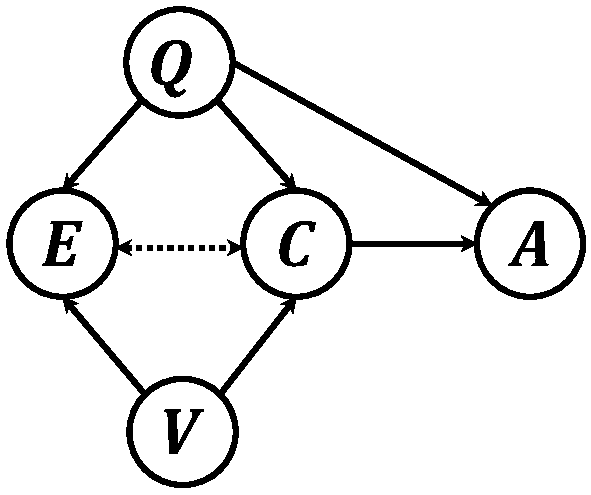
\includegraphics[scale=0.3]{fig/scm.pdf}
\vspace{-5pt}
\caption{Causal Graph of VideoQA}
\vspace{-10pt}
\label{fig:scm}
\end{figure}

\section{Methodology}
\label{sec:method}

\begin{figure*}[t]
\centering
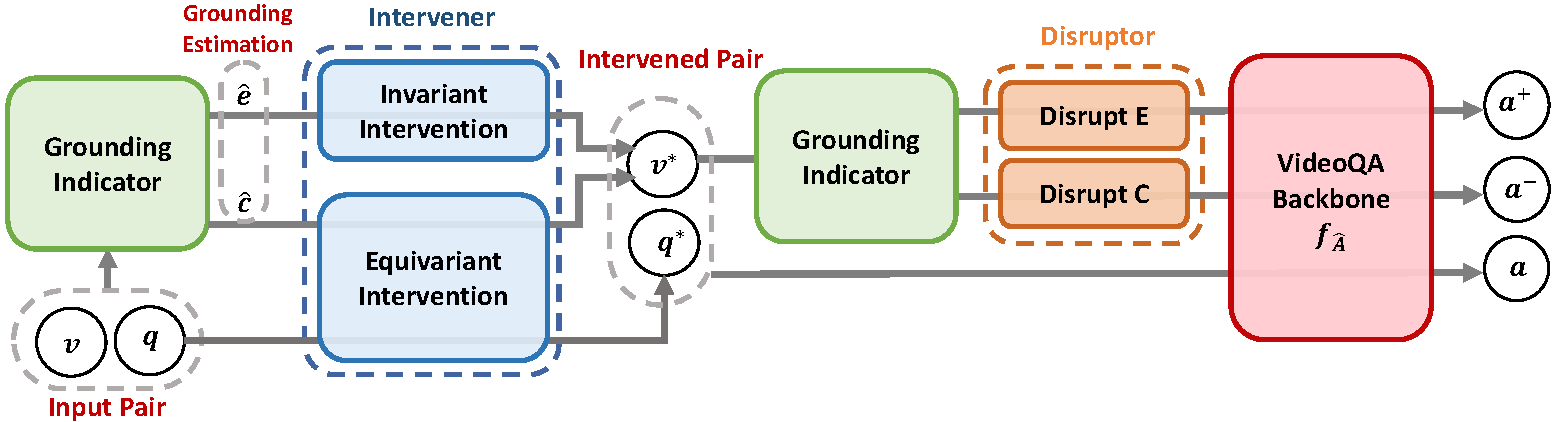
\includegraphics[width=0.95\textwidth]{fig/main.pdf}
\vspace{-14pt}
\caption{Overview of EIGV. It comprises three additional modules on top of the conventional VideoQA backbone: 1) Grounding indicator, 2) Intervener, and 3) Disrupter. First, the grounding indicator learns the estimation of causal scene $\hat{c}$ and environment $\hat{e}$. Next, two interventions are imposed on the causal and non-causal factors to compose the intervened pair $(v^*,q^*)$. Finally, based on the re-grounded result, the disruptor creates contrastive samples, which are further feed into the VideoQA backbone.}
\vspace{-5pt}
\label{fig:main}
\end{figure*}

\wx{
To ground the causal scene $C$ in the video $V$, we take a closer look at the VideoQA SCM (\ie Figure \ref{fig:scm}a), and emphasize the essential differences between $C$ and $E$.
Specifically, given the causal scene $C$ and question $Q$, the answer $A$ is determined, regardless of the variations in the environment scene $E$:}
\begin{gather}\label{equ:eq0}
      A\bot E \mid C,Q,
\end{gather}
where $\bot$ denotes the probabilistic independence. 
%

\vspace{5pt}
\noindent\textbf{Rationalization.} 
During training, the oracle grounding rationale $C$ is out of reach, while only the input $(V, Q)$ pair and training target $A$ are observed. 
Such an absence motivates VideoQA to embrace video grounding in its modeling. 
Specifically, in light of question $Q$, the estimated causal scene $\hat{C}$ is grounded from the massive $V$ to approach the oracle $C$ and then generate prediction $\hat{A}$ via $Q \rightarrow A \leftarrow C$. 
To systematize this relation, the causal-equivariance principle introduces an equivariant transformation $T_\epsilon$ to each of the parent variables (\ie $C$ and $Q$), and expects a proportionate change in the response variable (\ie $A$). On top of SCM, we formally present such notions as:
\begin{gather}
    T_\epsilon(\hat{A})=f_{\hat{A}}(T_\epsilon(\hat{C}),T_\epsilon(Q)). \label{equ:equivariance}
\end{gather}
Meanwhile, environment-invariant principle formulated Equation \eqref{equ:eq0} in the sense that imposing an invariant-transformation $T_\iota$ on the estimated environment $\hat{E}$ should not trigger variation of answer $A$: 
\begin{gather}
      \hat{A}=f_{\hat{A}}(T_\iota(\hat{E}),Q)),\label{equ:invariance}
\end{gather} 
To this end, we parameterize our learning framework, EIGV, as a combination of equivariant and invariant principles, which comprises three additional modules on top of the ERM-guided backbone: grounding indicator, intervener, and disruptor. In a nutshell, we display our EIGV framework in Figure \ref{fig:main}.


\vspace{5pt}
\noindent \textbf{Data representation.}
Following previous efforts \cite{jiang2020reasoning, DBLP:conf/acl/GuoZJ0L20}, we encode video instance $v$ as a sequence of $K$ fixed visual clips, while question instance $q$ is encoded into a similar form with a fixed length of language tokens $L$.
Then, visual and linguistic features are applied with a linear layer and an LSTM \cite{10.1162/neco.1997.9.8.1735}, respectively, to align their dimension. As a result, we acquire the output of linear layer $ \vb{v} \in \mathbb{R}^{k \times d}$ as the final video representation and the last hidden state of LSTM $\vb{q} \in \mathbb{R}^{d}$ as the holistic question representation.

% Following previous efforts [], video instance $v$ is encoded as a sequence of $K$ fixed visual clips $ \vb{v} \in \mathbb{R}^{k \times d_v}$, where $d_v$ is the visual feature dimension. Likewise, the question instance $q$ is encoded into similar form $ \vb{q} \in \mathbb{R}^{L \times d_q}$ but with a fixed length of language tokens L. Furthermore, $\vb{v}$ and $\vb{q}$ are respectively, applied with a linear layer and a LSTM [] to align their dimension, while we acquire the final hidden state of LSTM as a the holistic question representation $\vb{q} \in \mathbb{R}^{d}$.

\subsection{Grounding Indicator}
Scene partition is fundamental to the rationale discovery, whose core is to estimate the value of $C$ and $E$ via a hard split on video $V$. Given an input sample $(v,q)$, the grounding indicator aims to access the causal scene and environment scene via their estimated value $\hat{c}$ and $\hat{e}$ according to question $Q$. 
%
Concretely, we first construct two cross-modal attention modules to indicate the probability of each visual clip of being causal scene ($\vb{p}_{\hat{c}} \in\mathbb{R}^{K}$) 
and environment scene ($\vb{p}_{\hat{e}}\in\mathbb{R}^{K}$):
\begin{align}
    \vb{p}_{\hat{c}} &= \text{Softmax}(\text{FC}_{1}(\vb{v})\cdot\text{FC}_{2}(\vb{q})^\intercal),\\
    \vb{p}_{\hat{t}} &= \text{Softmax}(\text{FC}_{3}(\vb{v})\cdot\text{FC}_{4}(\vb{q})^\intercal),
\end{align}
where $\text{FC}_{1},\text{FC}_{2},\text{FC}_{3},\text{FC}_{4}$ are fully connected layers that align cross-modal representations.
%
However, gathering messages via a soft mask still makes the visual information on different clips overlap. 
As discussed in Section 3.2, guided by ERM, the conventional attention mechanism is unable to block the influence of $\hat{e}$, thus undermining the veracity of $\hat{c}$.
% As revealed by the ERM-guided method, the conventional attention is unable to block the influence of $\hat{t}$ thus undermining the veracity of $\hat{e}$. 
%
As a correction, the grounding indicator makes a discrete selection over the clip-wise attention result to generate a disjoint group of the causal scene. We leverage Gumbel-Softmax \cite{DBLP:conf/iclr/JangGP17} to manage a differentiable selection on attentive probabilities and compute the indicator vector $\vb{I}\in\mathbb{R}^{K\times 2}$ on the two attention scores  over each clip (\ie $\vb{p}_{\hat{c,i}}$, $\vb{p}_{\hat{e,i}}$, $i \in K$).  Formally, $\vb{I}$ is derived as:
\begin{gather}
    \vb{I} = \text{Gumbel-Softmax}([\vb{p}_{\hat{c}};\vb{p}_{\hat{e}}]), 
\end{gather}
where $[;]$ denote concatenation. The first and second column of $\vb{I}$ (\ie $I_{0}$ and $I_{1}$) index the attribution of $\hat{c}$ and $\hat{e}$ over k clips, respectively. 
%
To this end, we estimate $\hat{c}$ and $\hat{e}$ as follows:
\begin{gather}
    \hat{c} = I_{0}\cdot v ,\quad \hat{e} = I_{1}\cdot v, \quad \st v=\hat{c}+\hat{e} .
    % \hat{c} = \{I_{c,k}\cdot v_{k}|I_{c,k}=1\},\quad \hat{t} = \{I_{t,k}\cdot v_{k}|I_{t,k}=1\},
\end{gather}

% where binary masks $I_{0k}$ and $I_{1k}$ indicate the causal-environment attribution of the $k$-th clip.

\subsection{Intervener}
In absence of clip-level supervision, learning grounding indicators requires dedicated exploitation of the equivariance-invariance principle.
%
On this demand, we propose the intervener, which prompts the estimated rationale to the oracle by intervening $\hat{c}$ and $\hat{e}$. 
%
Figure \ref{fig:intervene} describes the functionality of $do(\cdot)$ --- the intervention operator that successively manipulated SCM over $E$ and $C$. Concretely, two intervention operations are configured to realize the equivariant and invariant transformation defined in Equations \eqref{equ:equivariance} and \eqref{equ:invariance}. 
%
% 这块儿写的不清楚。要牢记突出主线:two principle,所有的都是围绕这个实现的,只有我们反复强调这个,才能让reviewer印象深刻,然后才能从idea、implementation层面上都理解我们在干啥,并且觉得我们做的是对的。
% 这里可以分开写:

To fulfill the causal-equivariant principle, we design the E-intervention on the causal scene $\hat{c}$, which applies a linear interpolation between two data points on their causal factors --- $C$, $Q$ and $A$.  
By casting the same mixing ratio $\lambda_0\sim\text{Beta}(\alpha,\alpha)$ on all causal factors, the equivariant intervener learns to capture 
% the mainstay depicted in Figure \ref{fig:scm}c, so as to abridge 
the causal connection of $C, Q \to A$.
In particular, we attain the intervened causal scene $c^*\in \mathbb{R}^{K\times d}$, question $q^*\in \mathbb{R}^{d}$ and answer $a^*\in \mathbb{R}$ as follow:
\begin{gather}
    c^*=\lambda_0 \cdot \hat{c}+(1-\lambda_0) \cdot \hat{c}',\\
    q^*=\lambda_0 \cdot q+(1-\lambda_0) \cdot q',\\
    a^*=\lambda_0 \cdot a+(1-\lambda_0) \cdot a',
\end{gather}
where $\hat{c}'$, $q'$ and $a'$ are causal factors from a second sample.

To achieve the environment-invariant principle, we devise the I-intervention that adopts a similar mixing strategy to the environment scene $\hat{e}$. 
%
Notably, by drawing the mixing ratios $\lambda_1$ from a second distribution that is distinct from the equivariant one (\ie $\lambda_1\sim\text{U}(0,1)$), the invariant intervention learns to rule out the influence of environment scene on the answer, which essentially refines the ERM-guided scheme at our will. 
Formally, we arrive the intervened environment scene $e^*$ by:
\begin{gather}
    e^*=\lambda_1 \cdot \hat{e}+(1-\lambda_1) \cdot \hat{e}',
\end{gather}
where $\hat{e}'$ is the estimated environment scene of a second sample.

In practice, the equvariant and invariant intervention operations are performed in parallel on different parts of $v$, and the intervened video $v^* \in \mathbb{R}^{K\times d}$ is composed of $do(C=c^*)$ and $do(E=e^*)$:
% in a cascade manner:
\begin{gather}
    v^*=c^*+e^*.
\end{gather}

% where $\hat{c}'$ and $\hat{e}'$ are estimate causal and environment scene of dummy  sample ($v',q',a'$).  It's worth noticing that, the mixing ratios $\lambda_0$ and $\lambda_1$ for equivariant and invarinat intervention are drawn from two different distribution, $\lambda_0\sim\text{Beta}(\alpha,\alpha)$ and $\lambda_1\sim\text{U}(0,1)$.
% %
% To complete the reasoning logic, we also apply the equivariant intervention on other causal factors---$Q$ and $A$ to generate intervened question $q^*$ and answer target $a^*$:
% \begin{gather}
%     q^*=\lambda_0 \cdot \hat{q}+(1-\lambda_0) \cdot q',\\
%     a^*=\lambda_1 \cdot \hat{a}+(1-\lambda_1) \cdot a',
% \end{gather}
% Noticably, we cast the same equivariant mixing ratio $\lambda_0$ for $do(Q)$ and $do(A)$ to abridge the the causal connection of $C,Q \to A$. 

% 
\subsection{Disruptor}
% In state-of-the-art self-supervised learning (SSL) pre-training produces semantically good representations by encouraging them to be invariant under meaningful transformations prescribed from human knowledge. 

To fully exploit the privilege of the proposed principles, we employ contrastive learning as an auxiliary objective to establish a good representation that maintains the desired properties of $\hat{c}$ and $\hat{e}$. 
% discribe in  to the counterfactual substitution on $C$($E$). 
Specifically, we first compose a memory bank $\pi$ as a collection of visual clips from other training videos. Then, we apply the grounding indicator a second time on top of the intervened variables, where the re-grounded causal and environment scene are manipulated to set up the contrastive twins as follows:
\begin{itemize}[leftmargin=*]
% 介绍清楚,为啥相对于anchor而言就是positive的
\item In light of the environment-invariance principle, positive video is developed in the sense that changing the environment scene will not provoke disagreement in answer semantics.  Thus, the disruptor synthesizes a positive video $v^+$ by disrupting the $v^*$ on its environment part --- that is, replacing the environment scene with a random stratification sampled from the memory bank.\footnote{Note that the environment substitutes will not involve the question-relevant scenes, to avoid creating additional paths from $E$ to $A$.}  
% 介绍清楚,为啥相对于anchor而言是negaitve的
\item Built upon the causal-equivariance principle, the negative counterpart $v^-$ is created by a similar disruption but on the causal scene of $v^*$, where substitution on the question-critical causal part should raise inconsistency in answer space.
% \footnote{substitution of causal scene substitutes will not involve the question-relevant scenes, to avoid creating additional paths from $E$ to $A$.} 
%
Apart from the visual negatives, the disruptor also creates linguistic alternatives to enhance the distinctiveness of the vision-language alignment. Specifically, it disrupts the combination of the intervened input ($v^*, q^*$) and pairs the video with random sample question $q_r$ to create a second view of negative samples ($v^*, q_r$).
\end{itemize}
To this end, we attain the answer representation of anchor $\vb{a}$ and its contrastive counterparts $\vb{a}^+, \vb{a}^-$ by feeding the paired positive and negative samples to backbone VideoQA model $f_{\hat{A}}$: 
\begin{gather}
    \vb{a}=f_{\hat{A}}(v^*,q^*),\\
    \vb{a}^+=f_{\hat{A}}(v^+,q^*),\\
    \vb{a}^-=f_{\hat{A}}([(v^-,q^*);\,(v^*,q_r)]),
\end{gather}
where $[;]$ denotes concatenation.

Notably, EIGV is designed to be model-agnostic, which aims to promote any VideoQA backbone built on frame-level visual inputs.
%
% Since the architecture modification is beyond our intention, we verify the effectiveness of our design by marrying EIGV to SoTA VideoQA models. 




\subsection{Optimization}
By far, we set up the intervened vision-language instance ($v^*,q^*$) for a pair of input ($v,q$), and further constitute its contrastive counterparts based on the estimated grounding result. 
To steer the learning process away from the conventional ERM pitfall, we establish two learning objectives on top of their output $a, a^+, a^-$:

\begin{itemize}[leftmargin=*]
    \vspace{5pt}
    \item \noindent \textbf{Contrastive loss.} To reflect the invariant property of the environment scene while maintaining the distinctiveness of the causal scene, we borrow the definition of InfoNCE \cite{DBLP:journals/corr/abs-1807-03748}, and construct the contrastive objective as follows:
    \begin{gather}
        \mathcal{L}_{CL}=-log(\frac{\text{exp}{(a^\top a^+)}}{\text{exp}{(a^\top a^+)}\,+\sum_{n}^{N}\text{exp}{(a^\top a_n^-)}}),
    \end{gather}
    where $N$ is the number of negative samples, \lyc{$a_n^-$ denotes negative anwer generated by one of  negative samples.} 
    
    \vspace{5pt}
    \item \noindent \textbf{ERM loss.} 
    Estimating the rationale requires a robust causal connection from $V,Q$ to $A$. Thus, we imposed an entropy-based risk function \lyc{$\text{XE}(\cdot)$} on $(v^*,q^*)$ to approach the intervened answer $a^*$:
    \begin{gather}
        \mathcal{L}_{ERM}=\text{XE}(f_{\hat{A}}(v^*,q^*), a^*),
    \end{gather}
\end{itemize}

As a result, the overall training objective of EIGV is the aggregation of the forgoing risks:
\begin{gather}
   \mathcal{L}_{\text{EIGV}} = \mathbb{E}_{(v,q,a)\in\mathcal{O}}\mathcal{L}_{ERM} + \beta\mathcal{L}_{CL},
\end{gather}
where $\mathcal{O}$ is the set of training instances $(v,q)$ alongside their ground-truth answer $a$; $\beta$ is the hyper-parameter that balances the strength of contrastive learning. The joint optimization disentangles the mischief of environment scene, thus fulfilling the desired interpretation by locating the causal pattern. During inference, EIGV generates the predication $\hat{a}$ without the intervener and disruptor involved, and gives the interpretation $\hat{c}$ as the partition result of the grounding indicator.

% Specifically, by minizing the  the similarity between en-
% coded representations of the same video at two
% different speeds as well as minimize the sim-
% ilarity between different videos played at dif-
% ferent speeds, leveraging the fact that changing
% video speed does not change an action on both
% domains.


% an oracle interpretation $C$ should reflect the semantic variance of different $Q$ and trigger the corresponding change in $A$,

% video input tend to contain multiple visual scene, but only the question-relevant part contributes to the prediction while the rest is inconsequential to the reasoning logic.


\begin{figure}[t]
\centering
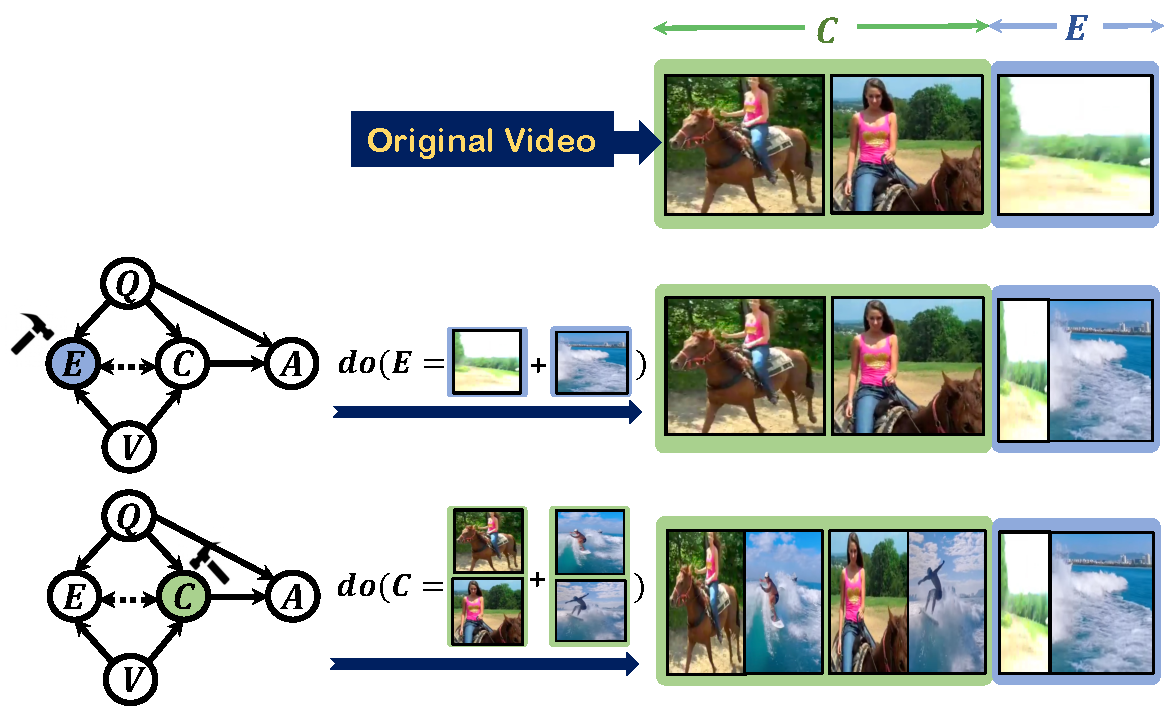
\includegraphics[scale=0.43]{fig/intervene.pdf}
\caption{We illustrate the invariant and equivariant interventions in the second and third rows, respectively. The effects on $Q$ and $A$ are omitted for illustration purposes.}
\vspace{-5pt}
\label{fig:intervene}
\end{figure}
\section{Experiment}
\label{sec:experiment}

In this section, we show the experimental results to answer the following research questions.
\begin{itemize}[leftmargin=*]
\item \textbf{RQ1} How effective is EIGV in discovering the causal pattern and improving the model generalization across different settings?
\item \textbf{RQ2} How does the sub-module and feature setting contribute to the performance?
\item \textbf{RQ3} What pattern does EIGV capture in rationale discovery?
\end{itemize}

\subsection{Settings}

\vspace{5pt}
\noindent \textbf{Datasets.} We conduct experiments on three benchmark datasets that challenge the model's reasoning capacity from different aspects: 
\textbf{MSVD-QA}  \cite{DBLP:conf/mm/XuZX0Z0Z17} and \textbf{MSRVTT-QA} \cite{DBLP:conf/mm/XuZX0Z0Z17} mainly emphasize the recognition ability by asking the descriptive questions, where 50K and 243K question-answer pairs are automatically generated from the human-labeled video captions, respectively.
\textbf{NExT-QA} \cite{DBLP:conf/cvpr/XiaoSYC21} pinpoints the causal and temporal relations among objects in the video. It contains 47.7K questions with answers in the form of multi-choice, which are manually annotated from 5.4K videos.

\vspace{5pt}
\noindent\textbf{Baseline.} We validate the effectiveness of EIGV across backbone VideoQA models of three kinds: 
1) \textbf{Memory-based} methods that foster a storage of input sequence via auxiliary memory design, such as AMU \cite{DBLP:conf/mm/XuZX0Z0Z17}, HME \cite{fan2019heterogeneous} and Co-Mem \cite{gao2018motionappearance}.
2) \textbf{Graph-based} methods that leverage the expressiveness of graph network to model the interaction between visual and language elements, which involves methods like L-GCN \cite{huang2020locationaware}, B2A  \cite{park2021bridge} and HGA \cite{jiang2020reasoning}. 
3) \textbf{Hierarchy-based} methods include HCRN \cite{le2021hierarchical}, PGAT \cite{DBLP:conf/mm/PengYBW21}, HOSTR \cite{dang2021hierarchical}, MSPAN \cite{DBLP:conf/acl/GuoZJ0L20} and HQGA \cite{xiao2021video}. In common, they exploit the multi-granularity nature of visual elements and realize the hierarchical reasoning via bottom-up architecture. 
In Specific, we test the generalization of EIGV by marrying our learning principles to three backbones of different categories: memory-based Co-Mem \cite{gao2018motionappearance}, graph-based HGA \cite{jiang2020reasoning} and hierarchy-based MSPAN \cite{DBLP:conf/acl/GuoZJ0L20}. 

\vspace{5pt}
\noindent \textbf{Implementation Detail.} 
For input representation, we encode the video instance as a sequence of $K$=16 clips, where each clip is represented as a combination of appearance and motion features extracted from the pre-trained ResNet-152 and 3D ResNeXt-101. For the linguistic feature, we follow \cite{DBLP:conf/cvpr/XiaoSYC21} and obtain the contextualized word representation using the fine-tuned BERT model. In the hyper-parameters setting, we set $d=512$ for cross-modal alignment, then train the model for 80 epochs with an initial learning rate of 5e-5.  During optimization, EIGV is trained with Adam optimizer and we decay the learning rate when validation stops improving for 5 epochs. The balance ratio $\beta$ is set to 0.75.
%for open-set QA and 0.025 for multi-choice QA. 

\subsection{Main Result (RQ1)}
\documentclass[lettersize,journal]{IEEEtran}
\usepackage{amsmath,amsfonts}
\usepackage{algorithmic}
\usepackage{algorithm}
\usepackage{array}
% \usepackage[caption=false,font=normalsize,labelfont=sf,textfont=sf]{subfig}
\usepackage{textcomp}
\usepackage{stfloats}
% \usepackage{xurl}
\usepackage{verbatim}
\usepackage{graphicx}
\usepackage{cite}
\usepackage{balance}
 
\usepackage{mathtools}
\usepackage{graphics, amsfonts, graphicx, amssymb, cite, mathrsfs}
% \let\proof\relax
% \let\endproof\relax
% \usepackage{amsthm}
% \usepackage{tikz}
% \usetikzlibrary{shapes,arrows}
% \usepackage{pgfplots}
\usepackage{color}
\usepackage[dvipsnames]{xcolor}
\usepackage{setspace}
% \usepackage[draft,bookmarks=false]{hyperref}
\usepackage{multirow}
\usepackage{rotating}
\usepackage{comment}
% \usepackage[keeplastbox]{flushend}
\usepackage[font=small]{caption}
% \usepackage{subcaption}
\usepackage[affil-it]{authblk}
% \usepackage{bm}
\usepackage{algorithm}
\usepackage{algorithmic}
\usepackage{enumitem}
% \usepackage{enumerate}
\usepackage{cite}
\usepackage{booktabs}
\usepackage{subcaption}
\usepackage{lipsum}

\PassOptionsToPackage{hyphens}{url}\usepackage{hyperref}

% \makeatletter
% \newcommand\fs@betterruled{%
%   \def\@fs@cfont{\bfseries}\let\@fs@capt\floatc@ruled
%   \def\@fs@pre{\vspace*{5pt}\hrule height.8pt depth0pt \kern2pt}%
%   \def\@fs@post{\kern2pt\hrule\relax}%
%   \def\@fs@mid{\kern2pt\hrule\kern2pt}%
%   \let\@fs@iftopcapt\iftrue}
% \floatstyle{betterruled}
% \restylefloat{algorithm}
% \makeatother


%
%%%%%%%%%%%%%%%%%%%%%%%%%%%%%%%%%theorem environments
%\newtheorem{assumption}{\hspace{0pt}\bf AS\hspace{-0.15cm}}
%\newtheorem{lemma}{\hspace{0pt}\bf Lemma}
%\newtheorem{proposition}{\hspace{0pt}\bf Proposition}
%\newtheorem{observation}{\hspace{0pt}\bf Observation}
%\newtheorem{theorem}{\hspace{0pt}\bf Theorem}
%\newtheorem{corollary}{\hspace{0pt}\bf Corollary}
%\newtheorem{fact}{\hspace{0pt}\bf Fact}
%\newtheorem{remark}{\hspace{0pt}\bf Remark}
%\newtheorem{test}{\hspace{0pt}\it Test Case}
%\newtheorem{definition}{\hspace{0pt}\bf Definition}
%\newtheorem{property}{\hspace{0pt}\bf Property}
%\newcommand {\mysubsubsection} [1] {\vspace{0.4cm}\noindent{\bf #1.}\addcontentsline{toc}{subsubsection}{\hspace{0pt}#1}}
%\newcommand {\mysubsection} [1]    {\vspace{0.4cm}\noindent{\bf #1.}\addcontentsline{toc}{subsection}{\hspace{0pt}#1}}



\newenvironment{myproof}[1][$\!\!$]{{\noindent\bf Proof #1: }}
                         {\hfill$\blacksquare$\medskip}

%%%%%%%%%%%%%%%%%%%%%%%%%%%%%%%%%list environment
\newenvironment{mylist}{\begin{list}{}{  \setlength{\itemsep  }{2pt} \setlength{\parsep    }{0in}
                                         \setlength{\parskip  }{0in} \setlength{\topsep    }{5pt}
                                         \setlength{\partopsep}{0in} \setlength{\leftmargin}{2pt}
                                         \setlength{\labelsep }{5pt} \setlength{\labelwidth}{-5pt}}}
                          {\end{list}\medskip}

\newcounter{excercise}
\newcounter{excercisepart}
\newcommand \excercise[1]{\addtocounter{excercise}{1} \setcounter{excercisepart}{0} \medskip
						  \noindent {\bf \theexcercise\ \, #1}}
\newcommand \excercisepart[1]{\addtocounter{excercisepart}{1} \medskip
						      \noindent {\it \Alph{excercisepart}\ \, #1}}


%%%%%%%%%%%%%%%%%%%%%%%%%%%%%%%%%list environment
%\newcounter{example}
%\newenvironment{example}[1]{\addtocounter{example}{1}\medskip \noindent{\it Example \theexample. #1.}}
%                           {\hfill\QED}%\newline\vspace{-2mm}\newline}


%%%%%%%%%%%%%%%%%%%%%%%%%%%%%%%%%slide equation environment
\newenvironment{slideeq} {              \begin{equation*}} {\end{equation*}            }
\newenvironment{nslideeq}{              \begin{equation*}} {\end{equation*}            }
\newenvironment{sslideeq}{\small        \begin{equation*}} {\end{equation*} \normalfont}
\newenvironment{fslideeq}{\footnotesize \begin{equation*}} {\end{equation*} \normalfont}
%%%%%%%%%%%%%%%%%%%%%%%%%%%%%%%%%slide equation environment
\newenvironment{slidealign} {              \begin{align*}} {\end{align*}            }
\newenvironment{nslidealign}{              \begin{align*}} {\end{align*}            }
\newenvironment{sslidealign}{\small        \begin{align*}} {\end{align*} \normalfont}
\newenvironment{fslidealign}{\footnotesize \begin{align*}} {\end{align*} \normalfont}

% Color definitions used in presentations
\definecolor{pennblue}{cmyk}{1,0.65,0,0.30}
\definecolor{pennred}{cmyk}{0,1,0.65,0.34}
\definecolor{mygreen}{rgb}{0.10,0.50,0.10}
\newcommand \red[1]         {{\color{red}#1}}
\newcommand \black[1]         {{\color{black}#1}}
\newcommand \blue[1]        {{\color{blue}#1}}
\newcommand \grey[1]        {{\color[rgb]{0.80,0.80,0.80}#1}}
\newcommand \gray[1]        {{\color[rgb]{0.80,0.80,0.80}#1}}
\newcommand \green[1]       {{\color[rgb]{0.10,0.50,0.10}#1}}
\newcommand \bulletcolor[1] {{\color{pennblue}#1}}
\def \arrowbullet {\bulletcolor{$\ \Rightarrow\ $}}
\def \arrbullet   {\bulletcolor{$\ \Rightarrow\ $}}
\def \ab          {\bulletcolor{$\ \Rightarrow\ $}}
\def \arritem     {\item[] \quad \arrowbullet}
\def \ai          {\item[] \quad \arrowbullet}
\def \doublearrow {\bulletcolor{$\ \Leftrightarrow\ $}}
\def \darrbullet  {\bulletcolor{$\ \Leftrightarrow\ $}}


%Always used
\def \defQfunction 
        {Q(u):=(1/\sqrt{2\pi})\int_u^\infty e^{-u^2/2} du}
\def \intinfty  { \int_{-\infty}^{\infty} }

%%%%%%%%%%%%%%%%%%%%%%%%%%%%%%%%% Overline
%
\def \ovP {\overline{P}}
\def \ovl {\overline{l}}
\def \ovbbl {\overline{\bbl}}
\def \ovX {\overline{X}}
\def \ovbbX {\overline{\bbX}}
\def \ovp {\overline{p}}
\def \ovbbp {\overline{\bbp}}
\def \ovr {\overline{r}}
\def \ova {\overline{a}}
\def \ovc {\overline{c}}
\def \ovalpha {\overline{\alpha}}

%%%%%%%%%%%%%%%%%%%%%%%%%%%%%%%%% Underline
%
\def \undP {\underline{P}}
\def \undl {\underline{l}}
\def \undbbl {\underline{\bbl}}
\def \undX {\underline{X}}
\def \undbbX {\underline{\bbX}}
\def \undp {\underline{p}}
\def \undbbp {\underline{\bbp}}
\def \undr {\underline{r}}
\def \unda {\underline{a}}
\def \undc {\underline{c}}
\def \undalpha {\underline{\alpha}}

%%%%%%%%%%%%%%%%%%%%%%%%%%%%%%%%% Overline and Underline
%
\def \undovP     {\underline{\ovP}}
\def \undovX     {\underline{\ovX}}
\def \undovbbX   {\underline{\ovbbX}}
\def \undovp     {\underline{\ovp}}
\def \undovbbp   {\underline{\ovbbp}}
\def \undovr     {\underline{\ovr}}
\def \undova     {\underline{\ova}}
\def \undovc     {\underline{\ovc}}
\def \undovalpha {\underline{\ovalpha}}

%roman symbols
\def \SNR     {\text{\normalfont SNR}   }
\def \ap      {\text{\normalfont ap}   }
\def \best    {\text{\normalfont best} }
\def \Co      {\text{\normalfont Co}   }
\def \Cov     {\text{\normalfont Cov}  }
\def \cov     {\text{\normalfont cov}  }
\def \dest    {\text{\normalfont dest} }
\def \diag    {\text{\normalfont diag} }
\def \eig     {\text{\normalfont eig}  }
\def \for     {\text{\normalfont for}  }
%\def \forall  {\text{\normalfont for all}  }
\def \forsome {\text{\normalfont for some}  }
\def \ML      {\text{\normalfont ML}   }
\def \MLE     {\text{\normalfont MLE}  }
\def \ml      {\text{\normalfont ml}   }
\def \mse     {\text{\normalfont mse}  }
\def \rank    {\text{\normalfont rank} }
\def \sign    {\text{\normalfont sign} }
\def \tr      {\text{\normalfont tr}   }

%units
\def \dB      {\, \text{\normalfont dB} }
\def \ms      {\, \text{\normalfont m}/ \text{\normalfont s}}
\def \kmh     {\, \text{\normalfont km}/ \text{\normalfont h}}
\def \m       {\, \text{\normalfont m} }
\def \s       {\, \text{\normalfont s} }
\def \sec     {\, \text{\normalfont sec.} }
\def \msec    {\, \text{\normalfont msec.} }
\def \cm      {\, \text{\normalfont cm} }
\def \km      {\, \text{\normalfont km} }
\def \GHz     {\, \text{\normalfont GHz} }
\def \Hz      {\, \text{\normalfont Hz} }
\def \MHZ     {\, \text{\normalfont MHz} }
\def \kHZ     {\, \text{\normalfont kHz} }


%Probability operators
\newcommand   \E     [1] {{\mathbb E}\left[#1\right]}
\newcommand   \Ec    [1] {{\mathbb E}\left(#1\right)}
\newcommand   \ind   [1] {{\mathbb I \left(#1\right)  } }
\renewcommand \Pr    [1] {\text{\normalfont Pr}  \left[#1\right]}
\newcommand   \Prc   [1] {\text{\normalfont Pr}  \left(#1\right)}
\renewcommand \P     [1] {\text{\normalfont P}   \left[#1\right]}
\newcommand   \Pc    [1] {\text{\normalfont P}   \left(#1\right)}
\newcommand   \Pcbig [1] {\text{\normalfont P}   \big(#1 \big)}
\newcommand   \PcBig [1] {\text{\normalfont P}   \Big(#1 \Big)}
\newcommand   \var   [1] {\text{\normalfont var} \left[#1\right]}
\newcommand   \varc  [1] {\text{\normalfont var} \left(#1\right)}
\renewcommand \Re    [1] {\text{\normalfont Re} \left(#1\right)}
\renewcommand \Im    [1] {\text{\normalfont Im} \left(#1\right)}
\newcommand   \der         [2] {\frac{\partial#1}{\partial#2}}
\newcommand   \inlineder   [2] {\partial#1/\partial#2}


%miscellaneous
\def \naturals {{\mathbb N}}
\def \reals    {{\mathbb R}}
\def \blog { {\bf \log   } }
\def \given{ {\,\big|\,  } }
\newcommand{\st}{\operatornamewithlimits{s.t.}}
\newcommand{\argmax}{\operatornamewithlimits{argmax}}
\newcommand{\argmin}{\operatornamewithlimits{argmin}}

%
%%%%%%%%%%%%%%%%%%%%%%%%%%%%%%%%%bar version
%capital alphabet
\def\bbarA{{\ensuremath{\bar A}}}
\def\bbarB{{\ensuremath{\bar B}}}
\def\bbarC{{\ensuremath{\bar C}}}
\def\bbarD{{\ensuremath{\bar D}}}
\def\bbarE{{\ensuremath{\bar E}}}
\def\bbarF{{\ensuremath{\bar F}}}
\def\bbarG{{\ensuremath{\bar G}}}
\def\bbarH{{\ensuremath{\bar H}}}
\def\bbarI{{\ensuremath{\bar I}}}
\def\bbarJ{{\ensuremath{\bar J}}}
\def\bbarK{{\ensuremath{\bar K}}}
\def\bbarL{{\ensuremath{\bar L}}}
\def\bbarM{{\ensuremath{\bar M}}}
\def\bbarN{{\ensuremath{\bar N}}}
\def\bbarO{{\ensuremath{\bar O}}}
\def\bbarP{{\ensuremath{\bar P}}}
\def\bbarQ{{\ensuremath{\bar Q}}}
\def\bbarR{{\ensuremath{\bar R}}}
\def\bbarW{{\ensuremath{\bar W}}}
\def\bbarU{{\ensuremath{\bar U}}}
\def\bbarV{{\ensuremath{\bar V}}}
\def\bbarS{{\ensuremath{\bar S}}}
\def\bbarT{{\ensuremath{\bar T}}}
\def\bbarX{{\ensuremath{\bar X}}}
\def\bbarY{{\ensuremath{\bar Y}}}
\def\bbarZ{{\ensuremath{\bar Z}}}
%lower case alphabet
\def\bbara{{\ensuremath{\bar a}}}
\def\bbarb{{\ensuremath{\bar b}}}
\def\bbarc{{\ensuremath{\bar c}}}
\def\bbard{{\ensuremath{\bar d}}}
\def\bbare{{\ensuremath{\bar e}}}
\def\bbarf{{\ensuremath{\bar f}}}
\def\bbarg{{\ensuremath{\bar g}}}
\def\bbarh{{\ensuremath{\bar h}}}
\def\bbari{{\ensuremath{\bar i}}}
\def\bbarj{{\ensuremath{\bar j}}}
\def\bbark{{\ensuremath{\bar k}}}
\def\bbarl{{\ensuremath{\bar l}}}
\def\bbarm{{\ensuremath{\bar m}}}
\def\bbarn{{\ensuremath{\bar n}}}
\def\bbaro{{\ensuremath{\bar o}}}
\def\bbarp{{\ensuremath{\bar p}}}
\def\bbarq{{\ensuremath{\bar q}}}
\def\bbarr{{\ensuremath{\bar r}}}
\def\bbarw{{\ensuremath{\bar w}}}
\def\bbaru{{\ensuremath{\bar u}}}
\def\bbarv{{\ensuremath{\bar v}}}
\def\bbars{{\ensuremath{\bar s}}}
\def\bbart{{\ensuremath{\bar t}}}
\def\bbarx{{\ensuremath{\bar x}}}
\def\bbary{{\ensuremath{\bar y}}}
\def\bbarz{{\ensuremath{\bar z}}}
%%%%%%%%%%%%%%%%%%%%%%%%%%%%%%%%%%end of bar version

%%%%%%%%%%%%%%%%%%%%%%%%%%%%%%%%%%%%%%%%%%%%%%%%%%%%%%%%%%%%%%%%%%%%%%%%%%%%%%%%%%%%%%%%%%%%%%%%
%%%   B   L   A   C   K   B   O   A   R   D         B   O   L   D   %%%%%%%%%%%%%%%%%%%%%%%%%%%%
%%%%%%%%%%%%%%%%%%%%%%%%%%%%%%%%%%%%%%%%%%%%%%%%%%%%%%%%%%%%%%%%%%%%%%%%%%%%%%%%%%%%%%%%%%%%%%%%
\def\mbA{{\ensuremath{\mathbb A}}}
\def\mbB{{\ensuremath{\mathbb B}}}
\def\mbC{{\ensuremath{\mathbb C}}}
\def\mbD{{\ensuremath{\mathbb D}}}
\def\mbE{{\ensuremath{\mathbb E}}}
\def\mbF{{\ensuremath{\mathbb F}}}
\def\mbG{{\ensuremath{\mathbb G}}}
\def\mbH{{\ensuremath{\mathbb H}}}
\def\mbI{{\ensuremath{\mathbb I}}}
\def\mbJ{{\ensuremath{\mathbb J}}}
\def\mbK{{\ensuremath{\mathbb K}}}
\def\mbL{{\ensuremath{\mathbb L}}}
\def\mbM{{\ensuremath{\mathbb M}}}
\def\mbN{{\ensuremath{\mathbb N}}}
\def\mbO{{\ensuremath{\mathbb O}}}
\def\mbP{{\ensuremath{\mathbb P}}}
\def\mbQ{{\ensuremath{\mathbb Q}}}
\def\mbR{{\ensuremath{\mathbb R}}}
\def\mbS{{\ensuremath{\mathbb S}}}
\def\mbT{{\ensuremath{\mathbb T}}}
\def\mbU{{\ensuremath{\mathbb U}}}
\def\mbV{{\ensuremath{\mathbb V}}}
\def\mbW{{\ensuremath{\mathbb W}}}
\def\mbX{{\ensuremath{\mathbb X}}}
\def\mbY{{\ensuremath{\mathbb Y}}}
\def\mbZ{{\ensuremath{\mathbb Z}}}
%%%%%%%%%%%%%%%%%%%%%%%%%%%%%%%%%%%%%%%%%%%%%%%%%%%%%%%%%%%%%%%%%%%%%%%%%%%%%%%%%%%%%%%%%%%%%%%%
%%%   C   A   L   I   G   R   A   P   H   I   C   %%%%%%%%%%%%%%%%%%%%%%%%%%%%%%%%%%%%%%%%%%%%%%
%%%%%%%%%%%%%%%%%%%%%%%%%%%%%%%%%%%%%%%%%%%%%%%%%%%%%%%%%%%%%%%%%%%%%%%%%%%%%%%%%%%%%%%%%%%%%%%%
\def\ccalA{{\ensuremath{\mathcal A}}}
\def\ccalB{{\ensuremath{\mathcal B}}}
\def\ccalC{{\ensuremath{\mathcal C}}}
\def\ccalD{{\ensuremath{\mathcal D}}}
\def\ccalE{{\ensuremath{\mathcal E}}}
\def\ccalF{{\ensuremath{\mathcal F}}}
\def\ccalG{{\ensuremath{\mathcal G}}}
\def\ccalH{{\ensuremath{\mathcal H}}}
\def\ccalI{{\ensuremath{\mathcal I}}}
\def\ccalJ{{\ensuremath{\mathcal J}}}
\def\ccalK{{\ensuremath{\mathcal K}}}
\def\ccalL{{\ensuremath{\mathcal L}}}
\def\ccalM{{\ensuremath{\mathcal M}}}
\def\ccalN{{\ensuremath{\mathcal N}}}
\def\ccalO{{\ensuremath{\mathcal O}}}
\def\ccalP{{\ensuremath{\mathcal P}}}
\def\ccalQ{{\ensuremath{\mathcal Q}}}
\def\ccalR{{\ensuremath{\mathcal R}}}
\def\ccalW{{\ensuremath{\mathcal W}}}
\def\ccalU{{\ensuremath{\mathcal U}}}
\def\ccalV{{\ensuremath{\mathcal V}}}
\def\ccalS{{\ensuremath{\mathcal S}}}
\def\ccalT{{\ensuremath{\mathcal T}}}
\def\ccalX{{\ensuremath{\mathcal X}}}
\def\ccalY{{\ensuremath{\mathcal Y}}}
\def\ccalZ{{\ensuremath{\mathcal Z}}}
%lower case alphabet
\def\ccala{{\ensuremath{\mathcal a}}}
\def\ccalb{{\ensuremath{\mathcal b}}}
\def\ccalc{{\ensuremath{\mathcal c}}}
\def\ccald{{\ensuremath{\mathcal d}}}
\def\ccale{{\ensuremath{\mathcal e}}}
\def\ccalf{{\ensuremath{\mathcal f}}}
\def\ccalg{{\ensuremath{\mathcal g}}}
\def\ccalh{{\ensuremath{\mathcal h}}}
\def\ccali{{\ensuremath{\mathcal i}}}
\def\ccalj{{\ensuremath{\mathcal j}}}
\def\ccalk{{\ensuremath{\mathcal k}}}
\def\ccall{{\ensuremath{\mathcal l}}}
\def\ccalm{{\ensuremath{\mathcal m}}}
\def\ccaln{{\ensuremath{\mathcal n}}}
\def\ccalo{{\ensuremath{\mathcal o}}}
\def\ccalp{{\ensuremath{\mathcal p}}}
\def\ccalq{{\ensuremath{\mathcal q}}}
\def\ccalr{{\ensuremath{\mathcal r}}}
\def\ccalw{{\ensuremath{\mathcal w}}}
\def\ccalu{{\ensuremath{\mathcal u}}}
\def\ccalv{{\ensuremath{\mathcal v}}}
\def\ccals{{\ensuremath{\mathcal s}}}
\def\ccalt{{\ensuremath{\mathcal t}}}
\def\ccalx{{\ensuremath{\mathcal x}}}
\def\ccaly{{\ensuremath{\mathcal y}}}
\def\ccalz{{\ensuremath{\mathcal z}}}
\def\ccal0{{\ensuremath{\mathcal 0}}}
%%%%%%%%%%%%%%%%%%%%%%%%%%%%%%%%%%%%%%%%%end of caligraph version
%
%
%%%%%%%%%%%%%%%%%%%%%%%%%%%%%%%%%%%%%%%%%%%hat version
%capital alphabet
\def\hhatA{{\ensuremath{\hat A}}}
\def\hhatB{{\ensuremath{\hat B}}}
\def\hhatC{{\ensuremath{\hat C}}}
\def\hhatD{{\ensuremath{\hat D}}}
\def\hhatE{{\ensuremath{\hat E}}}
\def\hhatF{{\ensuremath{\hat F}}}
\def\hhatG{{\ensuremath{\hat G}}}
\def\hhatH{{\ensuremath{\hat H}}}
\def\hhatI{{\ensuremath{\hat I}}}
\def\hhatJ{{\ensuremath{\hat J}}}
\def\hhatK{{\ensuremath{\hat K}}}
\def\hhatL{{\ensuremath{\hat L}}}
\def\hhatM{{\ensuremath{\hat M}}}
\def\hhatN{{\ensuremath{\hat N}}}
\def\hhatO{{\ensuremath{\hat O}}}
\def\hhatP{{\ensuremath{\hat P}}}
\def\hhatQ{{\ensuremath{\hat Q}}}
\def\hhatR{{\ensuremath{\hat R}}}
\def\hhatW{{\ensuremath{\hat W}}}
\def\hhatU{{\ensuremath{\hat U}}}
\def\hhatV{{\ensuremath{\hat V}}}
\def\hhatS{{\ensuremath{\hat S}}}
\def\hhatT{{\ensuremath{\hat T}}}
\def\hhatX{{\ensuremath{\hat X}}}
\def\hhatY{{\ensuremath{\hat Y}}}
\def\hhatZ{{\ensuremath{\hat Z}}}
%lower case alphabet
\def\hhata{{\ensuremath{\hat a}}}
\def\hhatb{{\ensuremath{\hat b}}}
\def\hhatc{{\ensuremath{\hat c}}}
\def\hhatd{{\ensuremath{\hat d}}}
\def\hhate{{\ensuremath{\hat e}}}
\def\hhatf{{\ensuremath{\hat f}}}
\def\hhatg{{\ensuremath{\hat g}}}
\def\hhath{{\ensuremath{\hat h}}}
\def\hhati{{\ensuremath{\hat i}}}
\def\hhatj{{\ensuremath{\hat j}}}
\def\hhatk{{\ensuremath{\hat k}}}
\def\hhatl{{\ensuremath{\hat l}}}
\def\hhatm{{\ensuremath{\hat m}}}
\def\hhatn{{\ensuremath{\hat n}}}
\def\hhato{{\ensuremath{\hat o}}}
\def\hhatp{{\ensuremath{\hat p}}}
\def\hhatq{{\ensuremath{\hat q}}}
\def\hhatr{{\ensuremath{\hat r}}}
\def\hhatw{{\ensuremath{\hat w}}}
\def\hhatu{{\ensuremath{\hat u}}}
\def\hhatv{{\ensuremath{\hat v}}}
\def\hhats{{\ensuremath{\hat s}}}
\def\hhatt{{\ensuremath{\hat t}}}
\def\hhatx{{\ensuremath{\hat x}}}
\def\hhaty{{\ensuremath{\hat y}}}
\def\hhatz{{\ensuremath{\hat z}}}
%%%%%%%%%%%%%%%%%%%%%%%%%%%%%%%%%%end of hat version
%
%
%%%%%%%%%%%%%%%%%%%%%%%%%%%%%%%%%%tilde version
%capital alphabet
\def\tdA{{\ensuremath{\tilde A}}}
\def\tdB{{\ensuremath{\tilde B}}}
\def\tdC{{\ensuremath{\tilde C}}}
\def\tdD{{\ensuremath{\tilde D}}}
\def\tdE{{\ensuremath{\tilde E}}}
\def\tdF{{\ensuremath{\tilde F}}}
\def\tdG{{\ensuremath{\tilde G}}}
\def\tdH{{\ensuremath{\tilde H}}}
\def\tdI{{\ensuremath{\tilde I}}}
\def\tdJ{{\ensuremath{\tilde J}}}
\def\tdK{{\ensuremath{\tilde K}}}
\def\tdL{{\ensuremath{\tilde L}}}
\def\tdM{{\ensuremath{\tilde M}}}
\def\tdN{{\ensuremath{\tilde N}}}
\def\tdO{{\ensuremath{\tilde O}}}
\def\tdP{{\ensuremath{\tilde P}}}
\def\tdQ{{\ensuremath{\tilde Q}}}
\def\tdR{{\ensuremath{\tilde R}}}
\def\tdW{{\ensuremath{\tilde W}}}
\def\tdU{{\ensuremath{\tilde U}}}
\def\tdV{{\ensuremath{\tilde V}}}
\def\tdS{{\ensuremath{\tilde S}}}
\def\tdT{{\ensuremath{\tilde T}}}
\def\tdX{{\ensuremath{\tilde X}}}
\def\tdY{{\ensuremath{\tilde Y}}}
\def\tdZ{{\ensuremath{\tilde Z}}}
%lower case alphabet
\def\tda{{\ensuremath{\tilde a}}}
\def\tdb{{\ensuremath{\tilde b}}}
\def\tdc{{\ensuremath{\tilde c}}}
\def\tdd{{\ensuremath{\tilde d}}}
\def\tde{{\ensuremath{\tilde e}}}
\def\tdf{{\ensuremath{\tilde f}}}
\def\tdg{{\ensuremath{\tilde g}}}
\def\tdh{{\ensuremath{\tilde h}}}
\def\tdi{{\ensuremath{\tilde i}}}
\def\tdj{{\ensuremath{\tilde j}}}
\def\tdk{{\ensuremath{\tilde k}}}
\def\tdl{{\ensuremath{\tilde l}}}
\def\tdm{{\ensuremath{\tilde m}}}
\def\tdn{{\ensuremath{\tilde n}}}
\def\tdo{{\ensuremath{\tilde o}}}
\def\tdp{{\ensuremath{\tilde p}}}
\def\tdq{{\ensuremath{\tilde q}}}
\def\tdr{{\ensuremath{\tilde r}}}
\def\tdw{{\ensuremath{\tilde w}}}
\def\tdu{{\ensuremath{\tilde u}}}
\def\tdv{{\ensuremath{\tilde r}}}
\def\tds{{\ensuremath{\tilde s}}}
\def\tdt{{\ensuremath{\tilde t}}}
\def\tdx{{\ensuremath{\tilde x}}}
\def\tdy{{\ensuremath{\tilde y}}}
\def\tdz{{\ensuremath{\tilde z}}}
%%%%%%%%%%%%%%%%%%%%%%%%%%%%%%%%%%%%end of tilde version
%
%%%%%%%%%%%%%%%%%%%%%%%%%%%%%%%%%%%%%check version
%lower case alphabet
\def\chka{{\ensuremath{\check a}}}
\def\chkb{{\ensuremath{\check b}}}
\def\chkc{{\ensuremath{\check c}}}
\def\chkd{{\ensuremath{\check d}}}
\def\chke{{\ensuremath{\check e}}}
\def\chkf{{\ensuremath{\check f}}}
\def\chkg{{\ensuremath{\check g}}}
\def\chkh{{\ensuremath{\check h}}}
\def\chki{{\ensuremath{\check i}}}
\def\chkj{{\ensuremath{\check j}}}
\def\chkk{{\ensuremath{\check k}}}
\def\chkl{{\ensuremath{\check l}}}
\def\chkm{{\ensuremath{\check m}}}
\def\chkn{{\ensuremath{\check n}}}
\def\chko{{\ensuremath{\check o}}}
\def\chkp{{\ensuremath{\check p}}}
\def\chkq{{\ensuremath{\check q}}}
\def\chkr{{\ensuremath{\check r}}}
\def\chkw{{\ensuremath{\check w}}}
\def\chku{{\ensuremath{\check u}}}
\def\chkv{{\ensuremath{\check v}}}
\def\chks{{\ensuremath{\check s}}}
\def\chkt{{\ensuremath{\check t}}}
\def\chkx{{\ensuremath{\check x}}}
\def\chky{{\ensuremath{\check y}}}
\def\chkz{{\ensuremath{\check z}}}
%%%%%%%%%%%%%%%%%%%%%%%%%%%%%%%%%%end of check version
%
%
%%%%%%%%%%%%%%%%%%%%%%%%%%%%%%%%%%%%Bold version
% upper case bold
\def\bbone{{\ensuremath{\mathbf 1}}}
\def\bbzero{{\ensuremath{\mathbf 0}}}
\def\bbA{{\ensuremath{\mathbf A}}}
\def\bbB{{\ensuremath{\mathbf B}}}
\def\bbC{{\ensuremath{\mathbf C}}}
\def\bbD{{\ensuremath{\mathbf D}}}
\def\bbE{{\ensuremath{\mathbf E}}}
\def\bbF{{\ensuremath{\mathbf F}}}
\def\bbG{{\ensuremath{\mathbf G}}}
\def\bbH{{\ensuremath{\mathbf H}}}
\def\bbI{{\ensuremath{\mathbf I}}}
\def\bbJ{{\ensuremath{\mathbf J}}}
\def\bbK{{\ensuremath{\mathbf K}}}
\def\bbL{{\ensuremath{\mathbf L}}}
\def\bbM{{\ensuremath{\mathbf M}}}
\def\bbN{{\ensuremath{\mathbf N}}}
\def\bbO{{\ensuremath{\mathbf O}}}
\def\bbP{{\ensuremath{\mathbf P}}}
\def\bbQ{{\ensuremath{\mathbf Q}}}
\def\bbR{{\ensuremath{\mathbf R}}}
\def\bbW{{\ensuremath{\mathbf W}}}
\def\bbU{{\ensuremath{\mathbf U}}}
\def\bbV{{\ensuremath{\mathbf V}}}
\def\bbS{{\ensuremath{\mathbf S}}}
\def\bbT{{\ensuremath{\mathbf T}}}
\def\bbX{{\ensuremath{\mathbf X}}}
\def\bbY{{\ensuremath{\mathbf Y}}}
\def\bbZ{{\ensuremath{\mathbf Z}}}
%lower case bold
\def\bba{{\ensuremath{\mathbf a}}}
\def\bbb{{\ensuremath{\mathbf b}}}
\def\bbc{{\ensuremath{\mathbf c}}}
\def\bbd{{\ensuremath{\mathbf d}}}
\def\bbe{{\ensuremath{\mathbf e}}}
\def\bbf{{\ensuremath{\mathbf f}}}
\def\bbg{{\ensuremath{\mathbf g}}}
\def\bbh{{\ensuremath{\mathbf h}}}
\def\bbi{{\ensuremath{\mathbf i}}}
\def\bbj{{\ensuremath{\mathbf j}}}
\def\bbk{{\ensuremath{\mathbf k}}}
\def\bbl{{\ensuremath{\mathbf l}}}
\def\bbm{{\ensuremath{\mathbf m}}}
\def\bbn{{\ensuremath{\mathbf n}}}
\def\bbo{{\ensuremath{\mathbf o}}}
\def\bbp{{\ensuremath{\mathbf p}}}
\def\bbq{{\ensuremath{\mathbf q}}}
\def\bbr{{\ensuremath{\mathbf r}}}
\def\bbw{{\ensuremath{\mathbf w}}}
\def\bbu{{\ensuremath{\mathbf u}}}
\def\bbv{{\ensuremath{\mathbf v}}}
\def\bbs{{\ensuremath{\mathbf s}}}
\def\bbt{{\ensuremath{\mathbf t}}}
\def\bbx{{\ensuremath{\mathbf x}}}
\def\bby{{\ensuremath{\mathbf y}}}
\def\bbz{{\ensuremath{\mathbf z}}}
\def\bb0{{\ensuremath{\mathbf 0}}}
%

% roman 
\def\rmA{{\ensuremath\text{A}}}
\def\rmB{{\ensuremath\text{B}}}
\def\rmC{{\ensuremath\text{C}}}
\def\rmD{{\ensuremath\text{D}}}
\def\rmE{{\ensuremath\text{E}}}
\def\rmF{{\ensuremath\text{F}}}
\def\rmG{{\ensuremath\text{G}}}
\def\rmH{{\ensuremath\text{H}}}
\def\rmI{{\ensuremath\text{I}}}
\def\rmJ{{\ensuremath\text{J}}}
\def\rmK{{\ensuremath\text{K}}}
\def\rmL{{\ensuremath\text{L}}}
\def\rmM{{\ensuremath\text{M}}}
\def\rmN{{\ensuremath\text{N}}}
\def\rmO{{\ensuremath\text{O}}}
\def\rmP{{\ensuremath\text{P}}}
\def\rmQ{{\ensuremath\text{Q}}}
\def\rmR{{\ensuremath\text{R}}}
\def\rmW{{\ensuremath\text{W}}}
\def\rmU{{\ensuremath\text{U}}}
\def\rmV{{\ensuremath\text{V}}}
\def\rmS{{\ensuremath\text{S}}}
\def\rmT{{\ensuremath\text{T}}}
\def\rmX{{\ensuremath\text{X}}}
\def\rmY{{\ensuremath\text{Y}}}
\def\rmZ{{\ensuremath\text{Z}}}
%lower case bold
\def\rma{{\ensuremath\text{a}}}
\def\rmb{{\ensuremath\text{b}}}
\def\rmc{{\ensuremath\text{c}}}
\def\rmd{{\ensuremath\text{d}}}
\def\rme{{\ensuremath\text{e}}}
\def\rmf{{\ensuremath\text{f}}}
\def\rmg{{\ensuremath\text{g}}}
\def\rmh{{\ensuremath\text{h}}}
\def\rmi{{\ensuremath\text{i}}}
\def\rmj{{\ensuremath\text{j}}}
\def\rmk{{\ensuremath\text{k}}}
\def\rml{{\ensuremath\text{l}}}
\def\rmm{{\ensuremath\text{m}}}
\def\rmn{{\ensuremath\text{n}}}
\def\rmo{{\ensuremath\text{o}}}
\def\rmp{{\ensuremath\text{p}}}
\def\rmq{{\ensuremath\text{q}}}
\def\rmr{{\ensuremath\text{r}}}
\def\rmw{{\ensuremath\text{w}}}
\def\rmu{{\ensuremath\text{u}}}
\def\rmv{{\ensuremath\text{v}}}
\def\rms{{\ensuremath\text{s}}}
\def\rmt{{\ensuremath\text{t}}}
\def\rmx{{\ensuremath\text{x}}}
\def\rmy{{\ensuremath\text{y}}}
\def\rmz{{\ensuremath\text{z}}}
%


%%%%%%%%%%%%%%%%%%%%%%%%%%%%%%%%%%%%%%%%%%%%%%bar bold version
%upper case
%
\def\barbA{{\bar{\ensuremath{\mathbf A}} }}
\def\barbB{{\bar{\ensuremath{\mathbf B}} }}
\def\barbC{{\bar{\ensuremath{\mathbf C}} }}
\def\barbD{{\bar{\ensuremath{\mathbf D}} }}
\def\barbE{{\bar{\ensuremath{\mathbf E}} }}
\def\barbF{{\bar{\ensuremath{\mathbf F}} }}
\def\barbG{{\bar{\ensuremath{\mathbf G}} }}
\def\barbH{{\bar{\ensuremath{\mathbf H}} }}
\def\barbI{{\bar{\ensuremath{\mathbf I}} }}
\def\barbJ{{\bar{\ensuremath{\mathbf J}} }}
\def\barbK{{\bar{\ensuremath{\mathbf K}} }}
\def\barbL{{\bar{\ensuremath{\mathbf L}} }}
\def\barbM{{\bar{\ensuremath{\mathbf M}} }}
\def\barbN{{\bar{\ensuremath{\mathbf N}} }}
\def\barbO{{\bar{\ensuremath{\mathbf O}} }}
\def\barbP{{\bar{\ensuremath{\mathbf P}} }}
\def\barbQ{{\bar{\ensuremath{\mathbf Q}} }}
\def\barbR{{\bar{\ensuremath{\mathbf R}} }}
\def\barbS{{\bar{\ensuremath{\mathbf S}} }}
\def\barbT{{\bar{\ensuremath{\mathbf T}} }}
\def\barbU{{\bar{\ensuremath{\mathbf U}} }}
\def\barbV{{\bar{\ensuremath{\mathbf V}} }}
\def\barbW{{\bar{\ensuremath{\mathbf W}} }}
\def\barbX{{\overline{\bbX}}}
\def\barbY{{\bar{\ensuremath{\mathbf Y}} }}
\def\barbZ{{\bar{\ensuremath{\mathbf Z}} }}
%
%lower case
%
\def\barba{{\bar{\ensuremath{\mathbf a}} }}
\def\barbb{{\bar{\ensuremath{\mathbf b}} }}
\def\barbc{{\bar{\ensuremath{\mathbf c}} }}
\def\barbd{{\bar{\ensuremath{\mathbf d}} }}
\def\barbe{{\bar{\ensuremath{\mathbf e}} }}
\def\barbf{{\bar{\ensuremath{\mathbf f}} }}
\def\barbg{{\bar{\ensuremath{\mathbf g}} }}
\def\barbh{{\bar{\ensuremath{\mathbf h}} }}
\def\barbi{{\bar{\ensuremath{\mathbf i}} }}
\def\barbj{{\bar{\ensuremath{\mathbf j}} }}
\def\barbk{{\bar{\ensuremath{\mathbf k}} }}
\def\barbl{{\bar{\ensuremath{\mathbf l}} }}
\def\barbm{{\bar{\ensuremath{\mathbf m}} }}
\def\barbn{{\bar{\ensuremath{\mathbf n}} }}
\def\barbo{{\bar{\ensuremath{\mathbf o}} }}
\def\barbp{{\bar{\ensuremath{\mathbf p}} }}
\def\barbq{{\bar{\ensuremath{\mathbf q}} }}
\def\barbr{{\bar{\ensuremath{\mathbf r}} }}
\def\barbs{{\bar{\ensuremath{\mathbf s}} }}
\def\barbt{{\bar{\ensuremath{\mathbf t}} }}
\def\barbu{{\bar{\ensuremath{\mathbf u}} }}
\def\barbv{{\bar{\ensuremath{\mathbf v}} }}
\def\barbw{{\bar{\ensuremath{\mathbf w}} }}
\def\barbx{{\bar{\ensuremath{\mathbf x}} }}
\def\barby{{\bar{\ensuremath{\mathbf y}} }}
\def\barbz{{\bar{\ensuremath{\mathbf z}} }}
%%%%%%%%%%%%%%%%%%%%%%%%%%%%%%%%%%%%%%%%%%%%%%%end of bar bold bersion
%
%
%%%%%%%%%%%%%%%%%%%%%%%%%%%%%%%%%%%%%%%%%%%%%%hat bold version
%upper case
%
\def\hbA{{\hat{\ensuremath{\mathbf A}} }}
\def\hbB{{\hat{\ensuremath{\mathbf B}} }}
\def\hbC{{\hat{\ensuremath{\mathbf C}} }}
\def\hbD{{\hat{\ensuremath{\mathbf D}} }}
\def\hbE{{\hat{\ensuremath{\mathbf E}} }}
\def\hbF{{\hat{\ensuremath{\mathbf F}} }}
\def\hbG{{\hat{\ensuremath{\mathbf G}} }}
\def\hbH{{\hat{\ensuremath{\mathbf H}} }}
\def\hbI{{\hat{\ensuremath{\mathbf I}} }}
\def\hbJ{{\hat{\ensuremath{\mathbf J}} }}
\def\hbK{{\hat{\ensuremath{\mathbf K}} }}
\def\hbL{{\hat{\ensuremath{\mathbf L}} }}
\def\hbM{{\hat{\ensuremath{\mathbf M}} }}
\def\hbN{{\hat{\ensuremath{\mathbf N}} }}
\def\hbO{{\hat{\ensuremath{\mathbf O}} }}
\def\hbP{{\hat{\ensuremath{\mathbf P}} }}
\def\hbQ{{\hat{\ensuremath{\mathbf Q}} }}
\def\hbR{{\hat{\ensuremath{\mathbf R}} }}
\def\hbS{{\hat{\ensuremath{\mathbf S}} }}
\def\hbT{{\hat{\ensuremath{\mathbf T}} }}
\def\hbU{{\hat{\ensuremath{\mathbf U}} }}
\def\hbV{{\hat{\ensuremath{\mathbf V}} }}
\def\hbW{{\hat{\ensuremath{\mathbf W}} }}
\def\hbX{{\hat{\ensuremath{\mathbf X}} }}
\def\hbY{{\hat{\ensuremath{\mathbf Y}} }}
\def\hbZ{{\hat{\ensuremath{\mathbf Z}} }}
%
%lower case
%
\def\hba{{\hat{\ensuremath{\mathbf a}} }}
\def\hbb{{\hat{\ensuremath{\mathbf b}} }}
\def\hbc{{\hat{\ensuremath{\mathbf c}} }}
\def\hbd{{\hat{\ensuremath{\mathbf d}} }}
\def\hbe{{\hat{\ensuremath{\mathbf e}} }}
\def\hbf{{\hat{\ensuremath{\mathbf f}} }}
\def\hbg{{\hat{\ensuremath{\mathbf g}} }}
\def\hbh{{\hat{\ensuremath{\mathbf h}} }}
\def\hbi{{\hat{\ensuremath{\mathbf i}} }}
\def\hbj{{\hat{\ensuremath{\mathbf j}} }}
\def\hbk{{\hat{\ensuremath{\mathbf k}} }}
\def\hbl{{\hat{\ensuremath{\mathbf l}} }}
\def\hbm{{\hat{\ensuremath{\mathbf m}} }}
\def\hbn{{\hat{\ensuremath{\mathbf n}} }}
\def\hbo{{\hat{\ensuremath{\mathbf o}} }}
\def\hbp{{\hat{\ensuremath{\mathbf p}} }}
\def\hbq{{\hat{\ensuremath{\mathbf q}} }}
\def\hbr{{\hat{\ensuremath{\mathbf r}} }}
\def\hbs{{\hat{\ensuremath{\mathbf s}} }}
\def\hbt{{\hat{\ensuremath{\mathbf t}} }}
\def\hbu{{\hat{\ensuremath{\mathbf u}} }}
\def\hbv{{\hat{\ensuremath{\mathbf v}} }}
\def\hbw{{\hat{\ensuremath{\mathbf w}} }}
\def\hbx{{\hat{\ensuremath{\mathbf x}} }}
\def\hby{{\hat{\ensuremath{\mathbf y}} }}
\def\hbz{{\hat{\ensuremath{\mathbf z}} }}
%%%%%%%%%%%%%%%%%%%%%%%%%%%%%%%%%%%%%%%%%%%%%%%end of hat bold  bersion
%
%
%%%%%%%%%%%%%%%%%%%%%%%%%%%%%%%%%%%%%%%%%%%%%%tilde bold version
%upper case
%
\def\tbA{{\tilde{\ensuremath{\mathbf A}} }}
\def\tbB{{\tilde{\ensuremath{\mathbf B}} }}
\def\tbC{{\tilde{\ensuremath{\mathbf C}} }}
\def\tbD{{\tilde{\ensuremath{\mathbf D}} }}
\def\tbE{{\tilde{\ensuremath{\mathbf E}} }}
\def\tbF{{\tilde{\ensuremath{\mathbf F}} }}
\def\tbG{{\tilde{\ensuremath{\mathbf G}} }}
\def\tbH{{\tilde{\ensuremath{\mathbf H}} }}
\def\tbI{{\tilde{\ensuremath{\mathbf I}} }}
\def\tbJ{{\tilde{\ensuremath{\mathbf J}} }}
\def\tbK{{\tilde{\ensuremath{\mathbf K}} }}
\def\tbL{{\tilde{\ensuremath{\mathbf L}} }}
\def\tbM{{\tilde{\ensuremath{\mathbf M}} }}
\def\tbN{{\tilde{\ensuremath{\mathbf N}} }}
\def\tbO{{\tilde{\ensuremath{\mathbf O}} }}
\def\tbP{{\tilde{\ensuremath{\mathbf P}} }}
\def\tbQ{{\tilde{\ensuremath{\mathbf Q}} }}
\def\tbR{{\tilde{\ensuremath{\mathbf R}} }}
\def\tbS{{\tilde{\ensuremath{\mathbf S}} }}
\def\tbT{{\tilde{\ensuremath{\mathbf T}} }}
\def\tbU{{\tilde{\ensuremath{\mathbf U}} }}
\def\tbV{{\tilde{\ensuremath{\mathbf V}} }}
\def\tbW{{\tilde{\ensuremath{\mathbf W}} }}
\def\tbX{{\tilde{\ensuremath{\mathbf X}} }}
\def\tbY{{\tilde{\ensuremath{\mathbf Y}} }}
\def\tbZ{{\tilde{\ensuremath{\mathbf Z}} }}
%
%lower case
%
\def\tba{{\tilde{\ensuremath{\mathbf a}} }}
\def\tbb{{\tilde{\ensuremath{\mathbf b}} }}
\def\tbc{{\tilde{\ensuremath{\mathbf c}} }}
\def\tbd{{\tilde{\ensuremath{\mathbf d}} }}
\def\tbe{{\tilde{\ensuremath{\mathbf e}} }}
\def\tbf{{\tilde{\ensuremath{\mathbf f}} }}
\def\tbg{{\tilde{\ensuremath{\mathbf g}} }}
\def\tbh{{\tilde{\ensuremath{\mathbf h}} }}
\def\tbi{{\tilde{\ensuremath{\mathbf i}} }}
\def\tbj{{\tilde{\ensuremath{\mathbf j}} }}
\def\tbk{{\tilde{\ensuremath{\mathbf k}} }}
\def\tbl{{\tilde{\ensuremath{\mathbf l}} }}
\def\tbm{{\tilde{\ensuremath{\mathbf m}} }}
\def\tbn{{\tilde{\ensuremath{\mathbf n}} }}
\def\tbo{{\tilde{\ensuremath{\mathbf o}} }}
\def\tbp{{\tilde{\ensuremath{\mathbf p}} }}
\def\tbq{{\tilde{\ensuremath{\mathbf q}} }}
\def\tbr{{\tilde{\ensuremath{\mathbf r}} }}
\def\tbs{{\tilde{\ensuremath{\mathbf s}} }}
\def\tbt{{\tilde{\ensuremath{\mathbf t}} }}
\def\tbu{{\tilde{\ensuremath{\mathbf u}} }}
\def\tbv{{\tilde{\ensuremath{\mathbf v}} }}
\def\tbw{{\tilde{\ensuremath{\mathbf w}} }}
\def\tbx{{\tilde{\ensuremath{\mathbf x}} }}
\def\tby{{\tilde{\ensuremath{\mathbf y}} }}
\def\tbz{{\tilde{\ensuremath{\mathbf z}} }}
%%%%%%%%%%%%%%%%%%%%%%%%%%%%%%%%%%%%%%%%%%%%%%%end of tilde bold  bersion
%
%%%%%%%%%%%%%%%%%%%%%%%%%%%%%%%%%%%%%%%%%%%%%%%bold caligraph
%
\def\bbcalA{\mbox{\boldmath $\mathcal{A}$}}
\def\bbcalB{\mbox{\boldmath $\mathcal{B}$}}
\def\bbcalC{\mbox{\boldmath $\mathcal{C}$}}
\def\bbcalD{\mbox{\boldmath $\mathcal{D}$}}
\def\bbcalE{\mbox{\boldmath $\mathcal{E}$}}
\def\bbcalF{\mbox{\boldmath $\mathcal{F}$}}
\def\bbcalG{\mbox{\boldmath $\mathcal{G}$}}
\def\bbcalH{\mbox{\boldmath $\mathcal{H}$}}
\def\bbcalI{\mbox{\boldmath $\mathcal{I}$}}
\def\bbcalJ{\mbox{\boldmath $\mathcal{J}$}}
\def\bbcalK{\mbox{\boldmath $\mathcal{K}$}}
\def\bbcalL{\mbox{\boldmath $\mathcal{L}$}}
\def\bbcalM{\mbox{\boldmath $\mathcal{M}$}}
\def\bbcalN{\mbox{\boldmath $\mathcal{N}$}}
\def\bbcalO{\mbox{\boldmath $\mathcal{O}$}}
\def\bbcalP{\mbox{\boldmath $\mathcal{P}$}}
\def\bbcalQ{\mbox{\boldmath $\mathcal{Q}$}}
\def\bbcalR{\mbox{\boldmath $\mathcal{R}$}}
\def\bbcalW{\mbox{\boldmath $\mathcal{W}$}}
\def\bbcalU{\mbox{\boldmath $\mathcal{U}$}}
\def\bbcalV{\mbox{\boldmath $\mathcal{V}$}}
\def\bbcalS{\mbox{\boldmath $\mathcal{S}$}}
\def\bbcalT{\mbox{\boldmath $\mathcal{T}$}}
\def\bbcalX{\mbox{\boldmath $\mathcal{X}$}}
\def\bbcalY{\mbox{\boldmath $\mathcal{Y}$}}
\def\bbcalZ{\mbox{\boldmath $\mathcal{Z}$}}
%
%%%%%%%%%%%%%%%%%%%%%%%%%%%%%%%%%%%%%%%%%%%%%%%%%%end of caligraph
%
%
%
%
%%%%%%%%%%%%%%%%%%%%%%%%%%%%%%%%%%%%%%%%%%%%%%%tilde Greek
%
\def\tdupsilon{\tilde\upsilon}
\def\tdalpha{\tilde\alpha}
\def\tbeta{\tilde\beta}
\def\tdgamma{\tilde\gamma}
\def\tddelta{\tilde\delta}
\def\tdepsilon{\tilde\epsilon}
\def\tdvarepsilon{\tilde\varepsilon}
\def\tdzeta{\tilde\zeta}
\def\tdeta{\tilde\eta}
\def\tdtheta{\tilde\theta}
\def\tdvartheta{\tilde\vartheta}

\def\tdiota{\tilde\iota}
\def\tdkappa{\tilde\kappa}
\def\tdlambda{\tilde\lambda}
\def\tdmu{\tilde\mu}
\def\tdnu{\tilde\nu}
\def\tdxi{\tilde\xi}
\def\tdpi{\tilde\pi}
\def\tdrho{\tilde\rho}
\def\tdvarrho{\tilde\varrho}
\def\tdsigma{\tilde\sigma}
\def\tdvarsigma{\tilde\varsigma}
\def\tdtau{\tilde\tau}
\def\tdupsilon{\tilde\upsilon}
\def\tdphi{\tilde\phi}
\def\tdvarphi{\tilde\varphi}
\def\tdchi{\tilde\chi}
\def\tdpsi{\tilde\psi}
\def\tdomega{\tilde\omega}

\def\tdGamma{\tilde\Gamma}
\def\tdDelta{\tilde\Delta}
\def\tdTheta{\tilde\Theta}
\def\tdLambda{\tilde\Lambda}
\def\tdXi{\tilde\Xi}
\def\tdPi{\tilde\Pi}
\def\tdSigma{\tilde\Sigma}
\def\tdUpsilon{\tilde\Upsilon}
\def\tdPhi{\tilde\Phi}
\def\tdPsi{\tilde\Psi}
%%%%%%%%%%%%%%%%%%%%%%%%%%%%%%%%%%%%%%%%%%%end of title  Greek
%
%%%%%%%%%%%%%%%%%%%%%%%%%%%%%%%%%%%%%%%%%%%%%%%bar Greek
%
\def\bbarupsilon{\bar\upsilon}
\def\bbaralpha{\bar\alpha}
\def\bbarbeta{\bar\beta}
\def\bbargamma{\bar\gamma}
\def\bbardelta{\bar\delta}
\def\bbarepsilon{\bar\epsilon}
\def\bbarvarepsilon{\bar\varepsilon}
\def\bbarzeta{\bar\zeta}
\def\bbareta{\bar\eta}
\def\bbartheta{\bar\theta}
\def\bbarvartheta{\bar\vartheta}

\def\bbariota{\bar\iota}
\def\bbarkappa{\bar\kappa}
\def\bbarlambda{\bar\lambda}
\def\bbarmu{\bar\mu}
\def\bbarnu{\bar\nu}
\def\bbarxi{\bar\xi}
\def\bbarpi{\bar\pi}
\def\bbarrho{\bar\rho}
\def\bbarvarrho{\bar\varrho}
\def\bbarvarsigma{\bar\varsigma}
\def\bbarphi{\bar\phi}
\def\bbarvarphi{\bar\varphi}
\def\bbarchi{\bar\chi}
\def\bbarpsi{\bar\psi}
\def\bbaromega{\bar\omega}

\def\bbarGamma{\bar\Gamma}
\def\bbarDelta{\bar\Delta}
\def\bbarTheta{\bar\Theta}
\def\bbarLambda{\bar\Lambda}
\def\bbarXi{\bar\Xi}
\def\bbarPi{\bar\Pi}
\def\bbarSigma{\bar\Sigma}
\def\bbarUpsilon{\bar\Upsilon}
\def\bbarPhi{\bar\Phi}
\def\bbarPsi{\bar\Psi}
%%%%%%%%%%%%%%%%%%%%%%%%%%%%%%%%%%%%%%%%%%%end of bar  Greek
%
%
%
%%%%%%%%%%%%%%%%%%%%%%%%%%%%%%%%%%%%%%%%%%%%%%%begion of check Greek
%
\def\chkupsilon{\check\upsilon}
\def\chkalpha{\check\alpha}
\def\chkbeta{\check\beta}
\def\chkgamma{\check\gamma}
\def\chkdelta{\check\delta}
\def\chkepsilon{\check\epsilon}
\def\chkvarepsilon{\check\varepsilon}
\def\chkzeta{\check\zeta}
\def\chketa{\check\eta}
\def\chktheta{\check\theta}
\def\chkvartheta{\check\vartheta}

\def\chkiota{\check\iota}
\def\chkkappa{\check\kappa}
\def\chklambda{\check\lambda}
\def\chkmu{\check\mu}
\def\chknu{\check\nu}
\def\chkxi{\check\xi}
\def\chkpi{\check\pi}
\def\chkrho{\check\rho}
\def\chkvarrho{\check\varrho}
\def\chksigma{\check\sigma}
\def\chkvarsigma{\check\varsigma}
\def\chktau{\check\tau}
\def\chkupsilon{\check\upsilon}
\def\chkphi{\check\phi}
\def\chkvarphi{\check\varphi}
\def\chkchi{\check\chi}
\def\chkpsi{\check\psi}
\def\chkomega{\check\omega}

\def\chkGamma{\check\Gamma}
\def\chkDelta{\check\Delta}
\def\chkTheta{\check\Theta}
\def\chkLambda{\check\Lambda}
\def\chkXi{\check\Xi}
\def\chkPi{\check\Pi}
\def\chkSigma{\check\Sigma}
\def\chkUpsilon{\check\Upsilon}
\def\chkPhi{\check\Phi}
\def\chkPsi{\check\Psi}
%%%%%%%%%%%%%%%%%%%%%%%%%%%%%%%%%%%%%%%%%%%end of check Greek
%
%
%
%%%%%%%%%%%%%%%%%%%%%%%%%%%%%%%%%%%%%%%%%%%%%%%%Bold Greek letter
%

\def\bbalpha{\boldsymbol{\alpha}}
\def\bbbeta{\boldsymbol{\beta}}
\def\bbgamma{\boldsymbol{\gamma}}
\def\bbdelta{\boldsymbol{\delta}}
\def\bbepsilon{\boldsymbol{\epsilon}}
\def\bbvarepsilon{\boldsymbol{\varepsilon}}
\def\bbzeta{\boldsymbol{\zeta}}
\def\bbeta{\boldsymbol{\eta}}
\def\bbtheta{\boldsymbol{\theta}}
\def\bbsigma{\boldsymbol{\sigma}}
\def\bbvartheta{\boldsymbol{\vartheta}}
\def \bbtau {\boldsymbol{\tau}}
\def\bbupsilon{\boldsymbol{\upsilon}}
\def\bbiota{\boldsymbol{\iota}}
\def\bbkappa{\boldsymbol{\kappa}}
\def\bblambda{\boldsymbol{\lambda}}
\def\bblam{\boldsymbol{\lambda}}
\def\bbmu{\boldsymbol{\mu}}
\def\bbnu{\boldsymbol{\nu}}
\def\bbxi{\boldsymbol{\xi}}
\def\bbpi{\boldsymbol{\pi}}
\def\bbrho{\boldsymbol{\rho}}
\def\bbvarrho{\boldsymbol{\varrho}}
\def\bbvarsigma{\boldsymbol{\varsigma}}
\def\bbphi{\boldsymbol{\phi}}
\def\bbvarphi{\boldsymbol{\varphi}}
\def\bbchi{\boldsymbol{\chi}}
\def\bbpsi{\boldsymbol{\psi}}
\def\bbomega{\boldsymbol{\omega}}
\def\bbGamma{\boldsymbol{\Gamma}}
\def\bbDelta{\boldsymbol{\Delta}}
\def\bbTheta{\boldsymbol{\Theta}}
\def\bbLambda{\boldsymbol{\Lambda}}
\def\bbXi{\boldsymbol{\Xi}}
\def\bbPi{\boldsymbol{\Pi}}
\def\bbSigma{\boldsymbol{\Sigma}}
\def\bbUpsilon{\boldsymbol{\Upsilon}}
\def\bbPhi{\boldsymbol{\Phi}}
\def\bbPsi{\boldsymbol{\Psi}}

%%%%%%%%%%%%%%%%%%%%%%%%%%%%%%%%%%%%%%%%%%%%%%%end of Bold Greek
%
%%%%%%%%%%%%%%%%%%%%%%%%%%%%%%%%%%%%%%%%%%%%%%bar Bold Greek
%
\def\barbupsilon{\bar\bbupsilon}
\def\barbalpha{\bar\bbalpha}
\def\barbbeta{\bar\bbbeta}
\def\barbgamma{\bar\bbgamma}
\def\barbdelta{\bar\bbdelta}
\def\barbepsilon{\bar\bbepsilon}
\def\barbvarepsilon{\bar\bbvarepsilon}
\def\barbzeta{\bar\bbzeta}
\def\barbeta{\bar\bbeta}
\def\barbtheta{\bar\bbtheta}
\def\barbvartheta{\bar\bbvartheta}

\def\barbiota{\bar\bbiota}
\def\barbkappa{\bar\bbkappa}
\def\barblambda{\bar\bblambda}
\def\barbmu{\bar\bbmu}
\def\barbnu{\bar\bbnu}
\def\barbxi{\bar\bbxi}
\def\barbpi{\bar\bbpi}
\def\barbrho{\bar\bbrho}
\def\barbvarrho{\bar\bbvarrho}
\def\barbvarsigma{\bar\bbvarsigma}
\def\barbphi{\bar\bbphi}
\def\barbvarphi{\bar\bbvarphi}
\def\barbchi{\bar\bbchi}
\def\barbpsi{\bar\bbpsi}
\def\barbomega{\bar\bbomega}

\def\barbGamma{\bar\bbGamma}
\def\barbDelta{\bar\bbDelta}
\def\barbTheta{\bar\bbTheta}
\def\barbLambda{\bar\bbLambda}
\def\barbXi{\bar\bbXi}
\def\barbPi{\bar\bbPi}
\def\barbSigma{\bar\bbSigma}
\def\barbUpsilon{\bar\bbUpsilon}
\def\barbPhi{\bar\bbPhi}
\def\barbPsi{\bar\bbPsi}
%%%%%%%%%%%%%%%%%%%%%%%%%%%%%%%%%%%%%%%%%%%end of bar Bold Greek
%
%%%%%%%%%%%%%%%%%%%%%%%%%%%%%%%%%%%%%%%%%%%%%%hat Bold Greek
%
\def\hbupsilon{\hat\bbupsilon}
\def\hbalpha{\hat\bbalpha}
\def\hbbeta{\hat\bbbeta}
\def\hbgamma{\hat\bbgamma}
\def\hbdelta{\hat\bbdelta}
\def\hbepsilon{\hat\bbepsilon}
\def\hbvarepsilon{\hat\bbvarepsilon}
\def\hbzeta{\hat\bbzeta}
\def\hbeta{\hat\bbeta}
\def\hbtheta{\hat\bbtheta}
\def\hbvartheta{\hat\bbvartheta}

\def\hbiota{\hat\bbiota}
\def\hbkappa{\hat\bbkappa}
\def\hblambda{\hat\bblambda}
\def\hbmu{\hat\bbmu}
\def\hbnu{\hat\bbnu}
\def\hbxi{\hat\bbxi}
\def\hbpi{\hat\bbpi}
\def\hbrho{\hat\bbrho}
\def\hbvarrho{\hat\bbvarrho}
\def\hbvarsigma{\hat\bbvarsigma}
\def\hbphi{\hat\bbphi}
\def\hbvarphi{\hat\bbvarphi}
\def\hbchi{\hat\bbchi}
\def\hbpsi{\hat\bbpsi}
\def\hbomega{\hat\bbomega}

\def\hbGamma{\hat\bbGamma}
\def\hbDelta{\hat\bbDelta}
\def\hbTheta{\hat\bbTheta}
\def\hbLambda{\hat\bbLambda}
\def\hbXi{\hat\bbXi}
\def\hbPi{\hat\bbPi}
\def\hbSigma{\hat\bbSigma}
\def\hbUpsilon{\hat\bbUpsilon}
\def\hbPhi{\hat\bbPhi}
\def\hbPsi{\hat\bbPsi}
%%%%%%%%%%%%%%%%%%%%%%%%%%%%%%%%%%%%%%%%%%%end of hat Bold Greek
%
%%%%%%%%%%%%%%%%%%%%%%%%%%%%%%%%%%%%%%%%%%%%%%tilde Bold Greek
%
\def\tbupsilon{\tilde\bbupsilon}
\def\tbalpha{\tilde\bbalpha}
\def\tbbeta{\tilde\bbbeta}
\def\tbgamma{\tilde\bbgamma}
\def\tbdelta{\tilde\bbdelta}
\def\tbepsilon{\tilde\bbepsilon}
\def\tbvarepsilon{\tilde\bbvarepsilon}
\def\tbzeta{\tilde\bbzeta}
\def\tbeta{\tilde\bbeta}
\def\tbtheta{\tilde\bbtheta}
\def\tbvartheta{\tilde\bbvartheta}

\def\tbiota{\tilde\bbiota}
\def\tbkappa{\tilde\bbkappa}
\def\tblambda{\tilde\bblambda}
\def\tbmu{\tilde\bbmu}
\def\tbnu{\tilde\bbnu}
\def\tbxi{\tilde\bbxi}
\def\tbpi{\tilde\bbpi}
\def\tbrho{\tilde\bbrho}
\def\tbvarrho{\tilde\bbvarrho}
\def\tbvarsigma{\tilde\bbvarsigma}
\def\tbphi{\tilde\bbphi}
\def\tbvarphi{\tilde\bbvarphi}
\def\tbchi{\tilde\bbchi}
\def\tbpsi{\tilde\bbpsi}
\def\tbomega{\tilde\bbomega}

\def\tbGamma{\tilde\bbGamma}
\def\tbDelta{\tilde\bbDelta}
\def\tbTheta{\tilde\bbTheta}
\def\tbLambda{\tilde\bbLambda}
\def\tbXi{\tilde\bbXi}
\def\tbPi{\tilde\bbPi}
\def\tbSigma{\tilde\bbSigma}
\def\tbUpsilon{\tilde\bbUpsilon}
\def\tbPhi{\tilde\bbPhi}
\def\tbPsi{\tilde\bbPsi}
%%%%%%%%%%%%%%%%%%%%%%%%%%%%%%%%%%%%%%%%%%%end of tilde Bold Greek
\def \deltat {\triangle t}
\def \eps    {\epsilon}
\def \lam    {\lambda}
\def \bblam  {\bblambda}
\def \Lam    {\Lambda}
\def \bbLam  {\bbLambda}
%%%%%%%%%%%%%%%%%%%%%%%%%%%%%%%%%%%%%%%%%%%%%%hat greek
%
\def\hhattheta{\hat\theta}
%%%%%%%%%%%%%%%%%%%%%%%%%%%%%%%%%%%%%%%%%%%end of hat greek

\def \vneg {\vspace{-2cm}}


\usepackage{amsthm}

% \usepackage{theorem}
\newtheorem{assumption}{\hspace{0pt}\bf Assumption}
\newtheorem{lemma}{\hspace{0pt}\bf Lemma}
\newtheorem{proposition}{\hspace{0pt}\bf Proposition}
\newtheorem{example}{\hspace{0pt}\bf Example}
\newtheorem{observation}{\hspace{0pt}\bf Observation}
\newtheorem{theorem}{\hspace{0pt}\bf Theorem}
\newtheorem{corollary}{\hspace{0pt}\bf Corollary}
\newtheorem{fact}{\hspace{0pt}\bf Fact}
\newtheorem{remark}{\hspace{0pt}\bf Remark}
\newtheorem{test}{\hspace{0pt}\it Test Case}
\newtheorem{definition}{\hspace{0pt}\bf Definition}
\newtheorem{conj}{\hspace{0pt}\bf Conjecture}

\def\Fro{{\mathrm{F}}}
\def\df{{\nabla f}}
\def\tlmin{{\hat{\lambda}_{\min}}}
\def\beye{\mathbf{I}}
%\def\bbG{\mathcal{G}}
\date{\today}
\def\whp{\text{w.h.p}}
\def\E{\mathbb{E}}
\def\supp{\text{support}}


\newcommand{\f}{{\mathbf{f}}}
\newcommand{\W}{{W}}
\newcommand{\BW}{{\tilde{W}}}
\newcommand{\Lf}{{L_{\f}}}
\newcommand{\R}{{\mathbb{R}}}
\DeclareMathOperator*{\Min}{minimize}


\definecolor{forestgreen}{rgb}{0.13, 0.55, 0.13}
\definecolor{Gray}{gray}{0.9}

\usepackage{todonotes}
\setlength\marginparwidth{2cm}
\newcommand{\nn}[1]{{\textcolor{red}{[\textit{Navid: #1}]}}}
\newcommand{\me}[1]{{\textcolor{blue}{[\textit{Mark: #1}]}}}



%%%%%%%%%%%%%%%%%%%%%%%%%%%%%%%%%%%%%%%%%%%%%%%%%%%%%%%%%%%%%%%%%%%%%%%%%%%%%%%%%%%%%%%%
% BEGIN: Definitions of long mathematical expressions
%%%%%%%%%%%%%%%%%%%%%%%%%%%%%%%%%%%%%%%%%%%%%%%%%%%%%%%%%%%%%%%%%%%%%%%%%%%%%%%%%%%%%%%% 
% Resource allocation functions
\def \fph  {\bbf\big(\bbp(\bbH), \bbH\big)}
\def \Efph {\mbE\big[\fph\big]}
% Optimal power allocation functions
\def \fphstar  {\bbf\big(\bbp^*(\bbH),\bbH\big)}
\def \Efphstar {\mbE\big[\fphstar\big]}
% Slater's condition power allocation functions
\def \fphzero  {\bbf\big(\bbp_0(\bbH),\bbH\big)}
\def \Efphzero {\mbE\big[\fphzero\big]}
% Parametrized power allocation functions
\def \fphih  {\bbf\big(\bbphi(\bbH,\bbtheta),\bbH\big)}
\def \Efphih {\mbE\big[\fphih\big]}
\def \gphih  {g\big(\bbphi(\bbH,\bbtheta),\bbH\big)}
\def \Egphih {\mbE\big[\gphih\big]}
% Parametrized power allocation functions indexed by sample index k
\def \fpihk {\bbf\big(\bbH_k,\bbphi(\bbH_k,\bbtheta_k)\big)}
% Lagrangian
\def \Lagphi {\ccalL_{\bbphi}(\bbtheta,\bbx, \bblambda, \mu)}


\hyphenation{op-tical net-works semi-conduc-tor IEEE-Xplore}
% updated with editorial comments 8/9/2021

\begin{document}


% \title{Unsupervised Learning of State-Augmented Wireless Resource Management Policies}
% \title{Learning State-Augmented Algorithms for \\ Resource Management in Wireless Networks}
\title{State-Augmented Learnable Algorithms for Resource Management in Wireless Networks}

\author{}

\author{Navid~NaderiAlizadeh,
        Mark~Eisen,
        and~Alejandro~Ribeiro% <-this % stops a space
\thanks{N. NaderiAlizadeh and A. Ribeiro are with the Department of Electrical and Systems Engineering, University of Pennsylvania, Philadelphia,
PA 19104, USA (e-mails: \{nnaderi, aribeiro\}@seas.upenn.edu). M. Eisen is with Intel Labs, Intel Corporation, Hillsboro, OR 97124, USA (e-mail: mark.eisen@intel.com).

This work was supported in part by ARL DCIST CRA under Grant W911NF-17-2-0181, the AI Institute for Learning-Enabled Optimization at Scale (TILOS) (NSF CCF-2112665), and the NSF-Simons Research Collaboration on the Mathematical and Scientific Foundations of Deep Learning (MoDL) (NSF DMS-2031985).

This paper has been presented in part at the 2022 Asilomar Conference on Signals, Systems, and Computers~\cite{naderializadeh2022state}.}% <-this % stops a space
}

% % The paper headers
% \markboth{Journal of \LaTeX\ Class Files,~Vol.~14, No.~8, August~2021}%
% {Shell \MakeLowercase{\textit{et al.}}: A Sample Article Using IEEEtran.cls for IEEE Journals}

% \IEEEpubid{0000--0000/00\$00.00~\copyright~2021 IEEE}
% % Remember, if you use this you must call \IEEEpubidadjcol in the second
% % column for its text to clear the IEEEpubid mark.

\maketitle

\begin{abstract}
We consider resource management problems in multi-user wireless networks, which can be cast as optimizing a network-wide utility function, subject to constraints on the long-term average performance of users across the network. We propose a state-augmented algorithm for solving the aforementioned radio resource management (RRM) problems, where, alongside the instantaneous network state, the RRM policy takes as input the set of dual variables corresponding to the constraints, which evolve depending on how much the constraints are violated during execution. We theoretically show that the proposed state-augmented algorithm leads to feasible and near-optimal RRM decisions. Moreover, focusing on the problem of wireless power control using graph neural network (GNN) parameterizations, we demonstrate the superiority of the proposed RRM algorithm over baseline methods across a suite of numerical experiments.
\end{abstract}

\begin{IEEEkeywords}
Radio resource management, wireless networks, graph neural networks, Lagrangian duality, state augmentation, wireless power control.
\end{IEEEkeywords}

\section{Introduction}

With the proliferation of 5G network implementations across the globe and research already underway for future 6G wireless networks, novel wireless services and capabilities are expected to emerge that require carefully-optimized management of wireless resources. 
% Given the rising demand for wireless services with the advent of 5G networks, optimal resource allocation in wireless networks become of critical importance. 
Aside from traditional approaches for addressing such radio resource management (RRM) problems~\cite{shi2011iteratively, wu2013flashlinq, naderializadeh2014itlinq, yi2015itlinq+,shen2017fplinq}, learning-based methods have recently gained significant traction and demonstrated superior performance over prior approaches~\cite{eisen2019learning, nasir2019multi, liang2019deep, eisen2020optimal, shen2020graph, naderializadeh2021resource}. Such methods are envisioned to play a key role in current and future wireless networks with the ubiquitous availability of computational resources both at the end-user devices and within the network infrastructure~\cite{niknam2020intelligent,bonati2021intelligence,letaief2021edge,MediaTek_6G_whitepaper_2022}.

As a general formulation of the RRM problem, similarly to prior work~\cite{ribeiro2012optimal,eisen2019learning, eisen2020optimal, naderializadeh2022learning}, we consider a network utility maximization problem, subject to multiple constraints, where both the utility and the constraints are defined based on the long-term average performance of users across the network. A common method for solving such problems is to move to the Lagrangian dual domain, where a single objective, i.e., the Lagrangian, can be maximized over the primal variables and minimized over the dual variables, with each dual variable corresponding to a constraint in the original RRM problem. It can be shown that under mild conditions, such problems have null duality gap, hence allowing the use of primal-dual methods to derive optimal solutions. Even with the introduction of parameterizations for the RRM policy, the duality gap remains small in case of near-universal parameterizations, such as fully-connected deep neural networks. Nevertheless, such primal-dual algorithms lack feasibility guarantees---even for the case of convex optimization---except for an \emph{infinite} number of primal-dual iterations~\cite{nedic2009subgradient}. More precisely, it is unclear whether they lead to RRM decisions that satisfy the constraints in the original RRM problem if the training procedure is terminated after a finite number of iterations.

In this paper, we propose an alternative approach to solve the aforementioned constrained RRM problem. In particular, we leverage the fact that dual variables in constrained optimization provide indication of how much the corresponding constraints have been violated or satisfied over time. Using this observation, we incorporate the notion of \emph{state augmentation} from~\cite{calvo2021state}, in which the standard wireless network state is augmented with dual variables at each time instance to use as dynamic inputs to the RRM policy. By incorporating dual variables as an augmented input for the RRM policy, we are able to train the policy to adapt its decisions to not only instantaneous channel states, but also to such indications of constraint satisfaction. We theoretically establish two important properties of the proposed \emph{state-augmented} algorithm, which distinguish it from standard primal-dual training methods: the proposed algorithm leads to a trajectory of RRM decisions that are i) \emph{feasible}, i.e., satisfy the constraints almost-surely, and ii) \emph{near-optimal}, in the sense that the expected resulting network utility is within a constant additive gap of the optimum.

% We then dynamically update the dual variables during execution based on how much the corresponding constraints have been violated or satisfied. Borrowing  As shown in~\cite{calvo2021state}, such state augmentation is necessary when learning the policy directly is not necessarily possible.

As a prominent use case of the aforementioned state-augmented algorithm for solving RRM problems, we consider the problem of power control in multi-user interference channels, where the goal is to maximize the network sum-rate, subject to per-user minimum-rate requirements. We model the network state as the set of channel gains at each time step, and use a graph neural network (GNN) parameterization for the RRM policy, that takes as input both the network state and the dual variables at each time step, and outputs the transmit power levels. Through numerical experiments, we show that our proposed state-augmented algorithm, while slightly sacrificing the average performance, significantly outperforms baseline methods in terms of the worst-case user rates, thanks to satisfying the per-user minimum-rate constraints. We also show the benefits of the GNN-based parameterization of the RRM policy in terms of scalability to larger configurations and transferability to unseen network sizes, confirming the findings of prior work using such permutation-equivariant parameterizations~\cite{eisen2020optimal, lee2020graph, shen2020graph, naderializadeh2021wireless, chowdhury2021unfolding, wang2021unsupervised, chowdhury2021efficient, nikoloska2022modular, naderializadeh2022learning, li2022power, wang2022learning, zhao2022link}. It is important to note that GNNs are able to consider the relational structure among elements in an input graph when creating element-wise representations as opposed to other permutation-invariant/equivariant parameterizations in the set representation learning literature~\cite{zaheer2017deep, lee2019set, naderializadeh2021pooling, li2022heterogeneous}.

The rest of the paper is organized as follows. We begin in Section~\ref{sec:formulation} by formulating the radio resource management problem, in which instantaneous resource allocation decisions are made in response to network states to both maximize a utility and satisfy constraints on the long-term network performance. In Section~\ref{sec:param}, we show how parameterized RRM policies, trained via gradient-based methods, can lead to feasible RRM decisions that are optimal to within a constant additive gap by solving the problem in the Lagrangian dual domain. Such an algorithm is practically limited, however, due to, among other things, the large computational expense required during inference. 

In Section~\ref{sec:alg}, we describe our proposed approach of using state augmentation to learn alternative algorithms for RRM training and inference. We further prove its feasibility and near-optimality properties under proper assumptions on the expressive power of the state-augmented policy. In Section~\ref{sec:power_control}, we show the application of the proposed method to power control problems in multi-user interference channels with graph neural network parameterizations through an extensive series of numerical simulations. Finally, we conclude the paper in Section~\ref{sec:conclusion}.


\section{Problem Formulation}\label{sec:formulation}
We consider a wireless network operating over a series of time steps $t\in\{0,1,2,\dots,T-1\}$, where at each time step $t$, the set of channel gains in the network, or the \emph{network state}, is denoted by $\bbH_t \in \ccalH$. Given the network state, we let $\bbp(\bbH_t)$ denote the vector of \emph{radio resource management (RRM)} decisions across the network, where $\bbp : \ccalH \to \reals^a$ denotes the RRM function. These RRM decisions subsequently lead to the network-wide performance vector $\bbf(\bbH_t, \bbp(\bbH_t)) \in \reals^b$, with $\bbf: \ccalH \times \reals^a \to \reals^b$ denoting the performance function.

Given a concave utility $\mathcal{U}: \reals^b \to \reals$ and a set of $c$ concave constraints $\bbg: \reals^b \to \reals^c$, we define the generic RRM problem as
% \begin{subequations}\label{eq_param_problem}
% \begin{alignat}{2}
%     &\max_{\bbtheta,\bbx} &~~& \mathcal{U}(\bbx),             \\
%     &~~~\text{s.t.} && \bbx       \leq  \E_{\bbH} \left[ \bbf(\bbH, \bbp(\bbH;\bbtheta)) \right],   \label{eq:ergodic_rate_constraint}  \\
%     &&& \bbg(\bbx) \geq 0. \label{eq:min_rate_constraint_orig}%
% \end{alignat}
% \end{subequations}
\begin{subequations}\label{eq:nonparam_problem}
\begin{alignat}{2}
    &\max_{\{\bbp(\bbH_t)\}_{t=0}^{T-1}} &~~& \mathcal{U}\left( \frac{1}{T} \sum_{t=0}^{T-1} \bbf(\bbH_t, \bbp(\bbH_t)) \right),\label{eq:objective_non_param}             \\
    &~~~~~~\text{s.t.} &&  \bbg\left( \frac{1}{T} \sum_{t=0}^{T-1} \bbf(\bbH_t, \bbp(\bbH_t)) \right) \geq \bbzero,%
\end{alignat}
\end{subequations}
where the objective and the constraints are derived based on the \emph{ergodic average} network performance $\frac{1}{T} \sum_{t=0}^{T-1} \bbf(\bbH_t, \bbp(\bbH_t))$ rather than the instantaneous performance. The goal of the RRM problem is, therefore, to derive the optimal vector of RRM decisions $\bbp(\bbH_t)$ for any given network state $\bbH_t \in \ccalH$.


\section{Parameterized Gradient-Based RRM Algorithms in the Dual Domain}\label{sec:param}
As~\eqref{eq:objective_non_param} shows, problem~\eqref{eq:nonparam_problem} entails an infinite-dimensional search over the set of RRM decisions $\bbp(\bbH)$ for any given network state $\bbH$, which is practically infeasible. Therefore, we resort to \emph{parameterizing} the RRM policy and replacing $\bbp(\bbH)$ with $\bbp(\bbH;\bbtheta)$, where $\bbtheta \in \bbTheta$ denotes a finite-dimensional set of parameters. This, in turn, leads to the \emph{parameterized} RRM problem
\begin{subequations}\label{eq:param_problem}
\begin{alignat}{2}
    P^{\star}&=\max_{\bbtheta \in \bbTheta} &~~& \mathcal{U}\left( \frac{1}{T} \sum_{t=0}^{T-1} \bbf(\bbH_t, \bbp(\bbH_t;\bbtheta)) \right),             \\
    &~~~~~~\text{s.t.} &&   \bbg\left( \frac{1}{T} \sum_{t=0}^{T-1} \bbf(\bbH_t, \bbp(\bbH_t;\bbtheta)) \right)  \geq \bbzero, \label{eq:min_rate_constraint_param}%
\end{alignat}
\end{subequations}
where the maximization is now performed over the set of parameters $\bbtheta \in \bbTheta$.

In order to solve problem~\eqref{eq:param_problem}, we move to the Lagrangian dual domain. To derive the Lagrangian dual problem, we first introduce the Lagrangian function, with non-negative dual multipliers $\bbmu \in \reals_+^c$ associated with the constraints in \eqref{eq:min_rate_constraint_param}, as
%
\begin{align}
   \ccalL(\bbtheta, \bbmu) &= \mathcal{U}\left( \frac{1}{T} \sum_{t=0}^{T-1} \bbf(\bbH_t, \bbp(\bbH_t;\bbtheta)) \right)\nonumber \\
   &\qquad\qquad+ \bbmu^T \bbg\left( \frac{1}{T} \sum_{t=0}^{T-1} \bbf(\bbH_t, \bbp(\bbH_t;\bbtheta)) \right).\label{eq:param_lagrangian}
\end{align}
%
The Lagrangian in~\eqref{eq:param_lagrangian} can be optimized using gradient-based methods. In particular, we seek to maximize over $\bbtheta$, while subsequently minimizing over the dual multipliers $\bbmu$, i.e.,
%
\begin{align}\label{eq_dual_problem}
D^{\star} \coloneqq \min_{\bbmu \in \reals_+^c} \max_{\bbtheta \in \bbTheta} \ccalL(\bbtheta,\bbmu).
\end{align}
%
To train the model parameters $\bbtheta$, we introduce an \emph{iteration} duration $T_0$, which we define as the number of time steps between consecutive model parameter updates. Based on this notion, we define an iteration index $k\in\{0,1,2,\dots,K-1\}$ with $K=\lfloor T / T_0 \rfloor$, where the model parameters are updated as
\begin{align}
\bbtheta_k &= \arg \max_{\bbtheta\in\bbTheta} \Bigg[\mathcal{U}\left( \frac{1}{T_0} \sum_{t=kT_0}^{(k+1)T_0-1} \bbf(\bbH_{t}, \bbp(\bbH_{t};\bbtheta)) \right)\nonumber \\
  &\qquad\qquad+ \bbmu_{k}^T \bbg\left( \frac{1}{T_0} \sum_{t=kT_0}^{(k+1)T_0-1} \bbf(\bbH_{t}, \bbp(\bbH_{t};\bbtheta)) \right)\Bigg],\label{eq:theta_dynamics}
\end{align}
while the dual variables are updated recursively 
%at each time step $t\in\{0,1,2,\dots\}$ 
as
% based on which  we run the following dual gradient descent algorithm for each time step $t\in\{1,\dots,T\}$,
\begin{align}
% \bbtheta_t &= \arg \max_{\bbtheta\in\bbTheta} \ccalL(\bbtheta,\bbmu_t),\label{eq:theta_dynamics} \\
% \bbtheta_t &= \arg \max_{\bbtheta\in\bbTheta} \lim_{T\to\infty}\Bigg[\mathcal{U}\left( \frac{1}{T} \sum_{t'=t}^{t+T-1} \bbf(\bbH_{t'}, \bbp(\bbH_{t'};\bbtheta)) \right)\nonumber \\
%   &\qquad\qquad\qquad+ \bbmu_t^T \bbg\left( \frac{1}{T} \sum_{t'=t}^{t+T-1} \bbf(\bbH_{t'}, \bbp(\bbH_{t'};\bbtheta)) \right)\Bigg],\label{eq:theta_dynamics} \\
% \bbtheta_k &= \arg \max_{\bbtheta\in\bbTheta} \Bigg[\mathcal{U}\left( \frac{1}{T} \sum_{t'=kT}^{(k+1)T-1} \bbf(\bbH_{t'}, \bbp(\bbH_{t'};\bbtheta)) \right)\nonumber \\
%   &\qquad\qquad\qquad+ \bbmu_{kT}^T \bbg\left( \frac{1}{T} \sum_{t'=kT}^{(k+1)T-1} \bbf(\bbH_{t'}, \bbp(\bbH_{t'};\bbtheta)) \right)\Bigg],\label{eq:theta_dynamics} \\
% \bbmu_{t+1} &= \left[\bbmu_t - \eta_{\bbmu} \bbg\left(  \bbf(\bbH_t, \bbp(\bbH_t; \bbtheta_{\lfloor t / T_0 \rfloor})) \right)\right]_+,\label{eq:mu_dynamics}
\bbmu_{k+1} &= \left[\bbmu_k - \eta_{\bbmu} \bbg\left( \frac{1}{T_0} \sum_{t=kT_0}^{(k+1)T_0-1} \bbf(\bbH_{t}, \bbp(\bbH_{t};\bbtheta_k)) \right)\right]_+,\label{eq:mu_dynamics}
\end{align}
where $[\cdot]_+$ denotes projection onto the non-negative orthant, i.e., $[\cdot]_+ \coloneqq \max(\cdot, 0)$, and $\eta_{\bbmu}$ denotes the learning rate corresponding to the dual variables $\bbmu$.

Given the aforementioned training procedure, we can establish the following result on the generated RRM decisions. We note that similar results have been proven in~\cite{ribeiro2010ergodic, calvo2021state}.

% \newpage

\begin{theorem}\label{thm:main}
\allowdisplaybreaks
Consider a RRM algorithm, in which the primal parameters $\bbtheta$ and the dual variables $\bbmu$ follow the dynamics in~\eqref{eq:theta_dynamics} and~\eqref{eq:mu_dynamics}, respectively. Assuming that
\begin{itemize}
\item there exists a positive constant $G>0$ such that for any $\bbx \in \reals^b$, we have $|g_i(\bbx)| \leq G, \forall i\in\{1,\dots,c\}$; and,
\item there exists a strictly-feasible set of model parameters  $\hat{\bbtheta}$ such that $\bbg\left( \frac{1}{T} \sum_{t=0}^{T-1} \bbf(\bbH_t, \bbp(\bbH_t;\hat{\bbtheta})) \right) \geq G'\bbone$ for some positive constant $G'>0$,
\end{itemize}
then the resulting RRM decisions satisfy the desired constraints, i.e.,
\begin{align}\label{eq:thm_feasibility}
\lim_{T\to\infty}\bbg\left( \frac{1}{T} \sum_{t=0}^{T-1} \bbf(\bbH_t, \bbp(\bbH_t;\bbtheta_{\lfloor t/T_0 \rfloor})) \right) \geq \bbzero, \qquad a.s.
\end{align}
and they are within a constant additive gap of the optimum, i.e.,
\begin{align}
\lim_{T\to\infty} \hspace{-3pt} \E\left[ \mathcal{U}\left( \frac{1}{T} \sum_{t=0}^{T-1} \bbf(\bbH_t, \bbp(\bbH_t ;\bbtheta_{\lfloor t / T_0 \rfloor})) \right)\right]\hspace{-3pt} \geq\hspace{-2pt} P^{\star} \hspace{-3pt} - \frac{c\eta_{\bbmu}G^2}{2}.\label{eq:thm_optimality}
\end{align}

% {\color{teal}
% \begin{align}
% &\lim_{K\to\infty} \E\left[ \frac{1}{K} \sum_{k=1}^K \mathcal{U}\left( \frac{1}{T_0} \sum_{t=kT_0}^{(k+1)T_0-1} \bbf(\bbH_t, \bbp(\bbH_t ;\bbtheta_{k})) \right)\right] \nonumber\\
% &\geq P^{\star} - \frac{c\eta_{\mu}G^2}{2}.
% \end{align}
% }

% {\color{teal}
% \begin{align}
% \lim_{T\to\infty} \mathcal{U}\left( \frac{1}{T} \sum_{t=1}^T \E\left[ \bbf(\bbH_t, \bbp(\bbH_t;\bbtheta_t)) \right] \right) \geq P^{\star} - \frac{c\eta_{\mu}G^2}{2}.
% \end{align}
% }




\end{theorem}

\begin{proof}
See Appendix~\ref{appx:proof}.
\end{proof}



Theorem~\ref{thm:main} shows that the resulting RRM algorithm is both feasible and near-optimal if it is run for a large-enough number of time steps. This is notable, as with regular primal-dual methods, the RRM policies are not guaranteed to lead to a feasible set of RRM decisions, while such a feasibility guarantee exists for the RRM algorithm in~\eqref{eq:theta_dynamics}-\eqref{eq:mu_dynamics}. Note that the main factor that distinguishes~\eqref{eq:theta_dynamics}-\eqref{eq:mu_dynamics} from regular primal-dual methods (see, e.g.,~\cite{eisen2019learning}) is the maximization step in~\eqref{eq:theta_dynamics}, which adapts the RRM policy parameters to the dual variables at each iteration. % \blue{Mark: maybe it is worth stating what distinguishes (5)-(6) from "regular primal-dual methods" that gives it superior convergence properties, i.e. the maximization step in (5)?} \nn{Added a sentence on that; please check.}
The feasibility and near-optimality result of Theorem~\ref{thm:main} can indeed be proven for any non-convex optimization problem (see Appendix~\ref{appx:convex_hull}).

Nevertheless, the iterative RRM algorithm in~\eqref{eq:theta_dynamics}-\eqref{eq:mu_dynamics} presents a set of challenges that make it unsuitable for use in practice. First, maximizing the Lagrangian in~\eqref{eq:theta_dynamics} requires non-causal knowledge of the network states in the future%(see the definition of the Lagrangian in~\eqref{eq:param_lagrangian})
---the optimization at the $k$\textsuperscript{th} iteration (i.e., time step $t=kT_0$) requires the knowledge of the system state from $t=kT_0$ to $t=(k+1)T_0-1$, i.e., $\{\bbH_t\}_{t=kT_0}^{(k+1)T_0-1}$---which is impossible to obtain during execution, even though it might be viable during the training phase. Second, as Theorem~\ref{thm:main} demonstrates, convergence to  feasible and near-optimal RRM performance is only obtained as operation time $T$ tends to infinity. Thus, training iterations cannot be stopped at a finite time step, as there may not exist an iteration index $k$ for which $\bbtheta_k$ (or alternatively, a time average of $\{\bbtheta_{k'}\}_{k'=0}^{k-1}$) is optimal or feasible. %\green{This rules out the possibility of training the policy offline}\blue{Mark: is this right?}\nn{Technically yes, if we are not using a state-augmented parameterization. But since our proposed algorithm in the next section is indeed trained offline, it might be better to remove this point here.}.
Finally, in the maximization problem in~\eqref{eq:theta_dynamics}, the optimal set of model parameters needs to be found at each time step for a different vector of dual variables $\bbmu_k$, which can be computationally expensive, especially during the execution phase. This underscores the need to construct an algorithm that does not require memorization of the model parameters $\bbtheta$ for any given set of dual variables $\bbmu$, which we discuss next.

% Using a regular primal-dual approach, we can learn the parameters $\bbtheta$ and the dual variables $\bbmu$ over an iteration index $k$ as follows:
% \begin{align}
% \bbtheta_{k+1} &= \bbtheta_k + \eta_{\bbtheta} \nabla_{\bbtheta} \Bigg[ \mathcal{U}\left( \frac{1}{T} \sum_{t=1}^T \bbf(\bbH_t, \bbp(\bbH_t;\bbtheta)) \right) \nonumber \\
% &\qquad\qquad\qquad + \bbmu_k^T \bbg\left( \frac{1}{T} \sum_{t=1}^T \bbf(\bbH_t, \bbp(\bbH_t;\bbtheta)) \right) \Bigg]\\
% % \bbx_{k+1} &= \bbx_k + \eta_{\bbx} \left[\nabla_{\bbx} \left(\mathcal{U}(\bbx) + \bbmu_k^T \bbg(\bbx)\right) - \bblambda_k \right]\\
% % \bblambda_{k+1} &= [\bblambda_k - \eta_{\bblambda} (\E_{\bbH} \left[ \bbf(\bbH, \bbp(\bbH;\bbtheta_k)) \right] - \bbx_k)]_+\\
% \bbmu_{k+1} &= \left[\bbmu_k - \eta_{\bbmu} \bbg\left( \frac{1}{T} \sum_{t=1}^T \bbf(\bbH_t, \bbp(\bbH_t;\bbtheta_k)) \right)\right]_+,\label{eq:orig_dual_dynamics}
% \end{align}
% where $[\cdot]_+ \coloneqq \max(\cdot, 0)$, and $\eta_{\bbtheta}$ and $\eta_{\bbmu}$, respectively, denote the learning rates corresponding to the primal and dual variables, $\bbtheta$ and $\bbmu$.


\begin{remark}
It is important to note that in addition to the constraints on the ergodic average network performance, the formulation and aforementioned primal-dual algorithm are also able to handle instantaneous constraints if they are convex. However, they cannot address non-convex instantaneous constrains on the network performance. Considering non-convex instantaneous constraints is an interesting research direction, which we leave for future work.
\end{remark}

\section{Proposed State-Augmented RRM Algorithm}\label{sec:alg}

% \nn{To be revised based on iteration indexing ...}

In light of the aforementioned challenges, we propose a 
%In this paper, we take a different approach than the aforementioned primal-dual approach. Inspired by~\cite{calvo2021state}, we use the dual dynamics in~\eqref{eq:orig_dual_dynamics} to learn a 
\emph{state-augmented} RRM algorithm, similarly to~\cite{calvo2021state}, where the network state $\bbH_t$ at each time step $t$ is augmented by the corresponding set of dual variables $\bbmu_{\lfloor t/T_0 \rfloor}$, which are simultaneously used as inputs to the RRM policy. In particular, we introduce an alternative parameterization for the RRM policy, in which we represent the RRM decisions $\bbp(\bbH)$ using the parameterization $\bbp(\bbH, \bbmu; \bbphi)$, where $\bbphi\in\bbPhi$ denotes the set of parameters of the state-augmented RRM policy.

% For any time step $t\in\{1,\dots,T\}$, 
% In particular, during training, we first sample $\bbmu$ randomly from the non-negative orthant $\reals_+^c$. Given $\bbmu$, 
For a set of dual variables $\bbmu \in \reals_+^c$, we define the \emph{augmented} Lagrangian as
\begin{align}
\ccalL_{\bbmu}(\bbphi) &= \mathcal{U}\left( \frac{1}{T} \sum_{t=0}^{T-1} \bbf(\bbH_t, \bbp(\bbH_t, \bbmu;\bbphi)) \right) \nonumber \\
&\quad+ \bbmu^T \bbg\left( \frac{1}{T} \sum_{t=0}^{T-1} \bbf(\bbH_t, \bbp(\bbH_t, \bbmu;\bbphi)) \right).\label{eq:augmented_Lagrangian}
\end{align}
Then, considering a probability distribution $p_{\bbmu}$ for the dual variables, we define the optimal state-augmented RRM policy as that which maximizes the expected augmented Lagrangian over the distribution of all dual parameters, i.e., 
\begin{align}
\bbphi^{\star} &= \arg \max_{\bbphi \in \bbPhi} \E_{\bbmu \sim p_{\bbmu}}\left[ \ccalL_{\bbmu}(\bbphi) \right]. \label{eq:phi_dynamics_augmented}
\end{align}

Utilizing the state-augmented policy parameterized by $\bbphi^{\star}$ in \eqref{eq:phi_dynamics_augmented}, we can obtain the Lagrangian-maximizing RRM decision $\bbp(\bbH, \bbmu; \bbphi)$ for each dual iterate $\bbmu = \bbmu_{k}$. We therefore substitute the two-step update sequence in \eqref{eq:theta_dynamics}-\eqref{eq:mu_dynamics} with the state-augmented version of the dual multiplier update, i.e., %\blue{Mark: I think it might be a bit confusing to say (12) replaces (5), because (5) defines an iterative update whereas (12) is a separate (offline) optimization. Rather, by solving (12), we can replace (5)-(6) with (13).}\nn{Agreed with your point and your rewording of this paragraph.}
\begin{align}
% \bbmu_{t+1} &= \left[\bbmu_t - \eta_{\bbmu} \bbg\left(  \bbf(\bbH_t, \bbp(\bbH_t, \bbmu_t; \bbphi^{\star})) \right)\right]_+.\label{eq:mu_dynamics_augmented}
\bbmu_{k+1} \hspace{-3pt} &= \hspace{-3pt} \left[\bbmu_k - \eta_{\bbmu} \bbg\left( \frac{1}{T_0} \hspace{-6pt} \sum_{t=kT_0}^{(k+1)T_0-1} \bbf(\bbH_{t}, \bbp(\bbH_{t},\bbmu_k;\bbphi^{\star})) \right)\right]_+\hspace{-7pt}.\label{eq:mu_dynamics_augmented}
\end{align}
Note in \eqref{eq:mu_dynamics_augmented} the usage of the state-augmented RRM policy $\bbp(\bbH_{t},\bbmu_k;\bbphi^{\star})$ under the current dual multiplier at iteration $k$. Thus, in solving for the optimal state-augmented policy in \eqref{eq:phi_dynamics_augmented}, we are effectively \emph{learning} a parameterized model that, in conjunction with \eqref{eq:mu_dynamics_augmented}, executes the dual descent method in \eqref{eq:theta_dynamics}-\eqref{eq:mu_dynamics}.

Indeed, the main reason that we consider the state-augmented parameterization $\bbp(\bbH, \bbmu; \bbphi)$ is to resolve the challenge of memorizing the model parameters for any given set of dual variables. This implies that we need parameterizations with enough expressive power so that the RRM decisions made via the set of parameters $\bbphi^{\star}$ in~\eqref{eq:phi_dynamics_augmented} can closely approximate the ones using the iterative model parameters $\{\bbtheta_k (\bbmu_k)\}_{k=0}^{K-1}$ in~\eqref{eq:theta_dynamics}, where we have made explicit the dependence of $\bbtheta_k$ on $\bbmu_k$, $\forall k\in\{0,1,2,\dots,K-1\}$. To that end, we focus on a specific class of parameterizations, referred to as \emph{near-universal} parameterizations, which we define next.

\begin{definition}\label{def:near_universality}
Consider arbitrary functions $\bbtheta: \reals_+^c \to \bbTheta$ and $\bbp: \ccalH \times \bbTheta \to \reals^a$. A parameterization $\bbp(\bbH, \bbmu; \bbphi)$ with $\bbphi \in \bbPhi$ is near-universal with degree $\epsilon > 0$ for functions $\bbp(\bbH; \bbtheta(\bbmu))$ if for any network state $\bbH \in \ccalH$ and any functions $\bbtheta$ and $\bbp$, there exists $\bbphi \in \bbPhi$ such that
\begin{align}
\E_{\bbmu \sim p_{\bbmu}}\left\| \bbp(\bbH, \bbmu; \bbphi) - \bbp(\bbH; \bbtheta(\bbmu)) \right\|_{\infty} \leq \epsilon.
\end{align}
\end{definition}

We also introduce an additional assumption on the Lipschitz continuity of the expected utility and performance functions, which we mention below.
\begin{assumption}\label{assumption:Lipschitz}
The utility $\mathcal{U}$ and performance function $\bbf$ are expectation-wise Lipschitz. More precisely%, given arbitrary sets of network states $\{\bbH_t\}_{t=0}^{T-1}$% and RRM decisions $\{\bbp(\bbH_t)\}_{t=0}^{T-1}$
% , there exists a constant $L_{\mathcal{U}}$ such that 
, for any pair of ergodic average rate vectors $\bbx_1$ and $\bbx_2$, %RRM decision functions $\bbp_1$ and $\bbp_2$, 
we have
% \begin{align}
% & \E \left| \mathcal{U}\left( \sum_{t=0}^{T-1} \frac{\bbf(\bbH_t, \bbp_1(\bbH_t))}{T} \right) - \mathcal{U}\left( \sum_{t=0}^{T-1} \frac{\bbf(\bbH_t, \bbp_2(\bbH_t))}{T} \right) \right| \nonumber \\
% & \leq L_{\mathcal{U}} \E \left\| \frac{1}{T}\sum_{t=0}^{T-1} \bbf(\bbH_t, \bbp_1(\bbH_t)) - \bbf(\bbH_t, \bbp_2(\bbH_t)) \right\|_{\infty}.
% \end{align}
\begin{align}\label{eq:Lipschitz_U_1}
& \E \left| \hspace{1pt} \mathcal{U}\left( \bbx_1 \right) - \mathcal{U}\left( \bbx_2 \right) \right| \leq \E \left\| \bbx_1 - \bbx_2\right\|_{\infty}.
\end{align}
Moreover, given an arbitrary network state $\bbH$, there exists a constant $M$ such that any pair of RRM decision functions $\bbp_1$ and $\bbp_2$, we have
\begin{align}
& \E \left\| \bbf(\bbH, \bbp_1(\bbH)) - \bbf(\bbH, \bbp_2(\bbH)) \right\|_{\infty} \nonumber \\
& \qquad\qquad\qquad\leq M \E \left\| \bbp_1(\bbH) - \bbp_2(\bbH) \right\|_{\infty}.
\end{align}
\end{assumption}

Note that in~\eqref{eq:Lipschitz_U_1}, we assume that the Lipschitz constant for the utility $\mathcal{U}$ is equal to $1$ without loss of generality, as the utility function in the original optimization problem can be scaled by any arbitrary factor without any impact on the solution. Having Definition~\ref{def:near_universality} and Assumption~\ref{assumption:Lipschitz}, we can now state the following theorem, which shows that the RRM decisions generated by the proposed state-augmented procedure in~\eqref{eq:phi_dynamics_augmented}-\eqref{eq:mu_dynamics_augmented} are close to the ones made by the original iterative RRM algorithm in~\eqref{eq:theta_dynamics}-\eqref{eq:mu_dynamics}.

\begin{theorem}\label{thm:near_universality_result}
Under the hypotheses of Theorem~\ref{thm:main}, Assumption~\ref{assumption:Lipschitz}, and assuming that the state-augmented parameterization $\bbp(\bbH, \bbmu; \bbphi)$ is near-universal with degree $\epsilon$ in the sense of Definition~\ref{def:near_universality}, the RRM decisions made by the state-augmented algorithm in~\eqref{eq:phi_dynamics_augmented}-\eqref{eq:mu_dynamics_augmented} are both feasible, i.e.,
\begin{align}\label{eq:thm_feasibility_state_augmented}
\lim_{T\to\infty}\bbg\left( \frac{1}{T} \sum_{t=0}^{T-1} \bbf\left(\bbH_t, \bbp\left(\bbH_t, \bbmu_{\lfloor t/T_0 \rfloor}; \bbphi^{\star}\right) \right) \right) \geq \bbzero, \quad a.s.
\end{align}
and near-optimal, i.e.,
\begin{align}
&\lim_{T\to\infty} \E\left[ \mathcal{U}\left( \frac{1}{T} \sum_{t=0}^{T-1} \bbf\left(\bbH_t, \bbp\left(\bbH_t, \bbmu_{\lfloor t/T_0 \rfloor}; \bbphi^{\star}\right) \right) \right)\right] \nonumber \\
&\geq P^{\star} - \frac{c\eta_{\mu}G^2}{2} - M \epsilon.\label{eq:thm_optimality_state_augmented}
\end{align}
\end{theorem}

\begin{proof}
See Appendix~\ref{appx:proof_state_augmented}.
\end{proof}


\begin{algorithm*}[t]
\caption{Training Phase for the State-Augmented RRM Algorithm}
    \label{alg:training}
    \begin{algorithmic}[1]
    \STATE {\bfseries Input:} Number of training iterations $N$, batch size $B$, number of time steps $T$, primal learning rate $\eta_{\bbphi}$.
    \STATE Initialize: $\bbphi_0$.
    \FOR{$n=0, \ldots, N-1$}
        \FOR{$b=0, \ldots, B-1$}
            \STATE
            Randomly sample $\bbmu_b \sim p_{\bbmu}$.
            \STATE
            Randomly generate a sequence of network states $\{H_{b,t}\}_{t=0}^{T-1}$.
            \FOR{$t=0, \ldots, T-1$}
                \STATE 
                Generate RRM decisions $\bbp\left(\bbH_{b,t}, \bbmu_b; \bbphi_n\right)$.
            \ENDFOR
            \STATE
            Calculate the augmented Lagrangian according to~\eqref{eq:augmented_Lagrangian}, i.e., $$\ccalL_{\bbmu_b}(\bbphi_n) = \mathcal{U}\left( \frac{1}{T} \sum_{t=0}^{T-1} \bbf\left(\bbH_{b,t}, \bbp\left(\bbH_{b,t}, \bbmu_b; \bbphi_n\right)\right) \right)  + \bbmu^T \bbg\left( \frac{1}{T} \sum_{t=0}^{T-1}\bbf\left(\bbH_{b,t}, \bbp\left(\bbH_{b,t}, \bbmu_b; \bbphi_n\right)\right) \right).$$
        \ENDFOR
        \STATE
        Update the model parameters according to~\eqref{eq:phi_sga}, i.e., $$\bbphi_{n+1} = \bbphi_n +  \frac{\eta_{\bbphi}}{B} \sum_{b=0}^{B-1} \nabla_{\bbphi} \ccalL_{\bbmu_b}(\bbphi_n).$$
    \ENDFOR
    \STATE
    $\bbphi^{\star} \gets \bbphi_N$.
    \STATE
    {\bfseries Return:} {Optimal model parameters $\bbphi^{\star}$.}
    \end{algorithmic}
\end{algorithm*}

\begin{algorithm*}[t]
\caption{Execution Phase for the State-Augmented RRM Algorithm}
    \label{alg:execution}
    \begin{algorithmic}[1]
    \STATE {\bfseries Input:} Optimal model parameters $\bbphi^{\star}$, sequence of network states $\{H_{t}\}_{t=0}^{T-1}$, iteration length $T_0$, dual learning rate $\eta_{\bbmu}$.
    \STATE Initialize: $\bbmu_0 \gets \bbzero, k \gets 0$.
    \FOR{$t=0, \ldots, T-1$}
        \STATE 
        Generate RRM decisions $\bbp_t \coloneqq \bbp\left(\bbH_{t}, \bbmu_k; \bbphi^{\star}\right)$.
        \IF{$t+1 \mod T_0 = 0$}
        \STATE
        Update the dual variables according to~\eqref{eq:mu_dynamics_augmented}, i.e., $$\bbmu_{k+1} = \left[\bbmu_k - \eta_{\bbmu} \bbg\left( \frac{1}{T_0} \sum_{t=kT_0}^{(k+1)T_0-1} \bbf(\bbH_{t}, \bbp(\bbH_{t},\bbmu_k;\bbphi^{\star})) \right)\right]_+.$$
        \STATE
        $k \gets k+1.$
        \ENDIF
    \ENDFOR
    \STATE
    {\bfseries Return:} {Sequence of RRM decisions $\{\bbp_t\}_{t=0}^{T-1}$.}
    \end{algorithmic}
\end{algorithm*}

% \nn{Near-universality assumption + theorem to be added.}

\subsection{Practical Considerations}% Implementation of the State-Augmented Training Procedure}

% While the maximization in~\eqref{eq:phi_dynamics_augmented} makes the dependence of the model parameters $\bbphi$ on the dual variables $\bbmu$ more structured, it still requires non-causal access to the future states, which is infeasible during execution. 
In order to resolve the maximization in~\eqref{eq:phi_dynamics_augmented} during the offline training phase, we use a gradient ascent-based approach to learn an optimal set of parameters $\bbphi^{\star}$, which can be frozen after training is complete and utilized during execution. In particular, during the training phase, for a batch of dual variables $\{\bbmu_b\}_{b=1}^B$, randomly sampled from the distribution $p_{\bbmu}$, we consider the \emph{empirical} version of the Lagrangian maximization problem in~\eqref{eq:phi_dynamics_augmented}, i.e.,
\begin{align}
\bbphi^{\star} &= \arg \max_{\bbphi \in \bbPhi} \frac{1}{B} \sum_{b=1}^B \ccalL_{\bbmu_b}(\bbphi), \label{eq:phi_training_in_practice}
\end{align}
which we iteratively solve using gradient ascent. More specifically, we randomly initialize the model parameters as $\bbphi_0$, and then update them over an iteration index $n\in\{0,1,2,\dots,N-1\}$ as
\begin{align}
\bbphi_{n+1} &= \bbphi_n +  \frac{\eta_{\bbphi}}{B} \sum_{b=0}^{B-1} \nabla_{\bbphi} \ccalL_{\bbmu_b}(\bbphi_n),\label{eq:phi_sga}
\end{align}
where $\eta_{\bbphi}$ denotes the learning rate corresponding to the model parameters $\bbphi$. With a slight abuse of notation, we denote the final set of model parameters (i.e., the outcome of~\eqref{eq:phi_sga} upon convergence) as $\bbphi^{\star}$. Note that to enhance the generalization capability of the trained model, for each set of dual variables $\bbmu_b, b\in\{0,1,2,\dots,B\}$, in the batch, we can also randomly sample a separate realization of the sequence of network states, i.e., $\{H_{b,t}\}_{t=0}^{T-1}$, from the underlying random process, allowing the model to be optimized over a \emph{family} of network realizations. The training procedure is summarized in Algorithm~\ref{alg:training}.

%\nn{We could also talk about a randomly sampled batch of channel gains at each training iteration (i.e., optimizing over a \emph{family} of network configurations)?}

% for each configuration, we  we  we follow the following procedure:
% \begin{enumerate}
%     \item Sample $\bbmu$ randomly from the non-negative orthant $\reals_+^c$. {\color{red}(better sampling method? maybe higher $\mu$ for users in worse channel conditions?%normalizing the GNN inputs?
%     )}
%     \item Maximize the augmented Lagrangian $$\ccalL_{\bbmu}(\bbtheta) = \mathcal{U}\left( \frac{1}{T} \sum_{t=1}^T \bbf(\bbH_t, \bbp(\bbH_t, \bbmu;\bbtheta)) \right) + \bbmu^T \bbg\left( \frac{1}{T} \sum_{t=1}^T \bbf(\bbH_t, \bbp(\bbH_t, \bbmu;\bbtheta)) \right)$$ using gradient ascent on $\bbtheta$.
% \end{enumerate}

% \subsection{Dual-Augmented Execution Procedure}

During execution, the dual dynamics are used to update the dual variables and generate the RRM decisions as follows: We initialize the dual variables as $\bbmu_0 = \bbzero$. For any time step $t\in\{0,1,2,\dots,T-1\}$, given the network state $\bbH_t$, we generate the RRM decisions using the state-augmented RRM policy $\bbp(\bbH_t, \bbmu_{\lfloor t / T_0 \rfloor};\bbphi^{\star})$. Then, we update the dual variables every $T_0$ time steps as in~\eqref{eq:mu_dynamics_augmented}.
% \begin{align}
% \bbmu_{t+1} &= \left[\bbmu_t - \eta_{\bbmu} \bbg\left(  \bbf(\bbH_t, \bbp(\bbH_t, \bbmu_t;\bbtheta)) \right)\right]_+.\label{eq:dual_dynamics}
% \end{align}
Note how the dual dynamics in~\eqref{eq:mu_dynamics_augmented} track the satisfaction of the original constraints in~\eqref{eq:min_rate_constraint_param}. In particular, if the RRM decisions at time step $t$ help satisfy the constraints, the dual variables are reduced. On the other hand, if the constraints are not satisfied at a given time step, the dual variables increase in value. The state-augmented execution procedure is summarized in Algorithm~\ref{alg:execution}.


% \begin{enumerate}
%     \item Initialize the dual variables $\bbmu_1 = \bbzero$.
%     \item for $t=1,2,\dots$, do:
%     \begin{itemize}
%         \item Generate channel $\bbH_t$.
%         \item Generate the RRM decisions $\bbp(\bbH_t, \bbmu_t;\bbtheta)$.
%         \item Update the dual variables:
%         \begin{align}
%         % \bbx_{t+1} &= \bbx_t + \eta_{\bbx} \left[\nabla_{\bbx} \left(\mathcal{U}(\bbx) + \bbmu_k^T \bbg(\bbx)\right) - \bblambda_t \right]\\
%         % \bblambda_{t+1} &= \left[\bblambda_t - \eta_{\bblambda} \left(\frac{1}{t} \sum_{\tau=1}^{t} \left[ \bbf(\bbH_{\tau}, \bbp(\bbH_{\tau}, \bblambda_{\tau}, \bbmu_{\tau};\bbtheta)) \right] - \bbx_t\right)\right]_+\\
%         % \bbmu_{t+1} &= [\bbmu_t - \eta_{\bbmu} g(\bbx_t)]_+.\\
%         \bbmu_{t+1} &= \left[\bbmu_t - \eta_{\bbmu} \bbg\left(  \bbf(\bbH_t, \bbp(\bbH_t, \bbmu_t;\bbtheta)) \right)\right]_+.\label{eq:dual_dynamic}
%         \end{align}
%     \end{itemize}
% \end{enumerate}

\begin{remark}
Note that during the training procedure, the choice of distribution $p_{\bbmu}$ for sampling the dual variables, alongside the fact that they are kept fixed for the entire $T$ time steps, can affect the optimal model parameters $\bbphi^{\star}$. As we will show in Section~\ref{sec:exp_results}, a uniform distribution provides a desirable performance in our experiments. However, according to the dual dynamics in~\eqref{eq:mu_dynamics_augmented}, sampling the dual variables from the dual descent trajectory might lead to superior performance. Such a distribution may also be dependent on the realization of the initial network state, i.e., $\bbH_0$. For example, in an interference channel, the dual variables are expected to be higher on average for users in poor channel conditions (i.e., those with low signal-to-noise ratio (SNR) or large incoming interference-to-noise ratio (INR) values) as compared to users in favorable channel conditions (i.e., those with high SNR or low incoming INR values). The problems of finding the best distribution for sampling dual variables during training, and whether and how to update them during the $T$ training time steps for a given network realization, are interesting research directions, which we leave as future work.
\end{remark}

\begin{remark}
The RRM decisions $\bbp\left(\bbH_t, \bbmu_{\lfloor t/T_0 \rfloor}; \bbphi^{\star}\right)$ generated by our proposed algorithm might be suboptimal before the convergence of the dual variables. This implies that it might be beneficial to either i) have a number of warm-up time steps at the beginning of the execution phase until optimal RRM decisions are generated, or ii) initialize the dual variables with their optimal levels, which can be possible for network realizations seen during training, but does not necessarily transfer across different network realizations.
\end{remark}


\pagebreak

\section{Application to Power Control with \\ Graph Neural Network Parameterizations}\label{sec:power_control}
As an important application of the RRM problem to showcase the capabilities of the proposed state-augmented learning algorithm, we consider the problem of power control in $m$-user interference channels. More precisely, we study networks comprising $m$ \emph{users}, i.e., transmitter-receiver pairs $\{(\mathsf{Tx}_i, \mathsf{Rx}_i)\}_{i=1}^m$, where each transmitter intends to communicate to its corresponding receiver, while causing interference at other receivers. In this setting, the network state at time step $t$, i.e., $\bbH_t\in\mathbb{C}^{m \times m}$, contains all channel gains in the network, where the channel gain between transmitter $\mathsf{Tx}_i$ and receiver $\mathsf{Rx}_j$ at time step $t$ is denoted by by $h_{ij, t}\in\mathbb{C}$. The RRM decisions $\bbp \in [0, P_{\max}]^m$ represent the transmit power levels of the transmitters, with $P_{\max}$ denoting the maximum transmit power. Moreover, the performance function $\bbf(\bbH_t, \bbp)\in\reals^m$ represents the receiver rates, where for each receiver $\mathsf{Rx}_i$, the rate at time step $t$ is given by
\begin{align}
f_i(\bbH_t, \bbp) = \log_2\left(1+\frac{p_i \left|h_{ii,t}\right|^2}{N + \sum_{j=1, j\neq i}^m p_j \left|h_{ji,t}\right|^2}\right),
\end{align}
where $N$ denotes the noise variance, and it is assumed that the receiver treats all incoming interference as noise~\cite{annapureddy2009gaussian,geng2015optimality}.

We use a sum-rate utility $\ccalU(\bbx)=\sum_{i=1}^m x_i$, and consider per-user minimum-rate requirements as the constraints. In particular, we consider $c=m$ constraints, where the $i$\textsuperscript{th} constraint is given by $g_i(\bbx) = x_i - f_{\min}$, with $f_{\min}$ denoting the minimum per-user rate requirement. Therefore, letting $\bbone_m$ denote an $m$-dimensional vector of $1$'s, the optimization problem in~\eqref{eq:nonparam_problem} can be rewritten as
\begin{subequations}\label{eq:nonparam_problem_power_control}
\begin{alignat}{2}
    &\max_{\{\bbp(\bbH_t)\}_{t=0}^{T-1}} &~~& \frac{1}{T} \sum_{t=0}^{T-1} \sum_{i=1}^m f_i(\bbH_t, \bbp(\bbH_t)) ,\label{eq:objective_non_param_power_onctrol}             \\
    &~~~~~~\text{s.t.} &&   \frac{1}{T} \sum_{t=0}^{T-1} \bbf(\bbH_t, \bbp(\bbH_t))  \geq f_{\min} \bbone_m,\label{eq:min_rate_constraint}\\
    &~~~~~~ &&  \bbp(\bbPi^T \bbH \bbPi) = \bbPi^T \bbp(\bbH), \forall \bbH\in\ccalH, \forall \bbPi\in\ccalS_m.\label{eq:perm_eq_constraint}%
\end{alignat}
\end{subequations}
Note that in~\eqref{eq:perm_eq_constraint}, we have explicitly added a constraint on the \emph{permutation equivariance} of the power control policy, with $\ccalS_m$ denoting the set of all $m \times m$ permutation matrices, i.e.,
\begin{align}
\ccalS_m \coloneqq \left\{ \bbPi \in \{0,1\}^{m \times m} : \bbPi \bbone_m = \bbPi^T \bbone_m = \bbone_m \right\}.
\end{align}
This motivates the use of graph neural network (GNN) parameterizations, since they satisfy the permutation equivariance architecture by definition. For the problem of processing signals on graphs, certain GNN architectures have been shown to satisfy the near-universality assumption for a class of continuous, equivariant functions~\cite{keriven2019universal, azizian2021expressive, keriven2021universality}. It follows that with the restriction in~\eqref{eq:perm_eq_constraint}, the hypotheses of Theorem~\ref{thm:near_universality_result} are satisfied, since the set of permutation-equivariant functions is convex.% These universality results are applicable to our setting, since the set of permutation-equivariant functions is convex.


\subsection{GNN-Based Parameterizations}

In order to parameterize the state-augmented RRM policy, as in prior work~\cite{shen2020graph, eisen2020optimal, lee2020graph, naderializadeh2022learning}, we use GNN architectures, which have been shown to provide several benefits, such as scalability and transferability, alongside their inherent permutation equivariance. We operate the GNN over a graph-structured format of the interference channel, defined as a graph $\ccalG_t=(\ccalV, \ccalE, \bby_t, w_t)$ at each time step $t$, where:
\begin{itemize}
\item $\ccalV=\{1,2,\dots,m\}$ denotes the set of graph nodes, with each node representing a user (i.e., transmitter-receiver pair) in the graph,
\item $\ccalE = \ccalV \times \ccalV$ denotes the set of directed graph edges,
\item $\bbY_t \in \reals^{m \times 1}$ denotes the initial node features, which we set to the dual variables associated to the users at each time step, i.e., $\bbY_t \coloneqq \bbmu_{\lfloor t / T_0 \rfloor}$, and
\item $w_t: \ccalE \to \reals$ denotes the function that maps each edge to its weight at time $t$, which we define as $w_t(i, j) \coloneqq \frac{1}{Z_t} \log\left(P_{\max}|h_{ij, t}|^2 / N\right)$, with $Z_t > 0$ representing a normalization factor.
\end{itemize}

Note how the aforementioned graph structure allows the implementation of the state-augmented architecture, where the GNN can take the dual variables corresponding to all the users as the input node features, and the network state as the input edge features. More precisely, we consider $L$ consecutive GNN message-passing layers, where the $l$\textsuperscript{th} layer, $l\in\{1,2,\dots,L\}$ transforms the node features at layer $l-1$, i.e., $\bbY_t^{l-1}\in\reals^{m \times F_{l-1}}$, to the node features at layer $l$, i.e., $\bbY_t^{l}\in\reals^{m \times F_{l}}$. In its most general form, for each node $v\in\ccalV$, the aforementioned update can be written as
\begin{align}
\bby_{v,t}^{l} = \bbPsi^l\left( \left\{\bby_{u,t}^{l-1}, w_t(u,v) \right\}_{u\in\ccalV: (u,v)\in\ccalE}; \bbphi^l\right),
\end{align}
where $\bbPsi^l(\cdot; \bbphi^l): \reals^{F_{l-1}} \to \reals^{F_{l}}$ denotes the message-passing GNN operator, parameterized by the set of parameters $\bbphi^l$. We use $\bbY_t^0 = \bbY_t$ (with $F_0=1$) as the initial node features. We also set $F_{L}=1$ to produce a scalar output feature per node, and we define the power control decisions as
\begin{align}\label{eq:final_power_levels_GNN}
\bbp\left(\bbH_t, \bbmu_{\lfloor t / T_0 \rfloor};\bbphi\right) \coloneqq P_{\max} \cdot \sigma\left( \bbY_t^L \right),
\end{align}
where $\bbphi \coloneqq \left\{\bbphi^l\right\}_{l=1}^L$, and $\sigma(\cdot)$ denotes element-wise sigmoid function, with $\sigma(x)=\frac{1}{1+\exp(-x)}, \forall x\in\reals$, which is used to respect the instantaneous power level constraints $\bbp \in [0, P_{\max}]^m$.


\begin{figure*}[h]
\centering
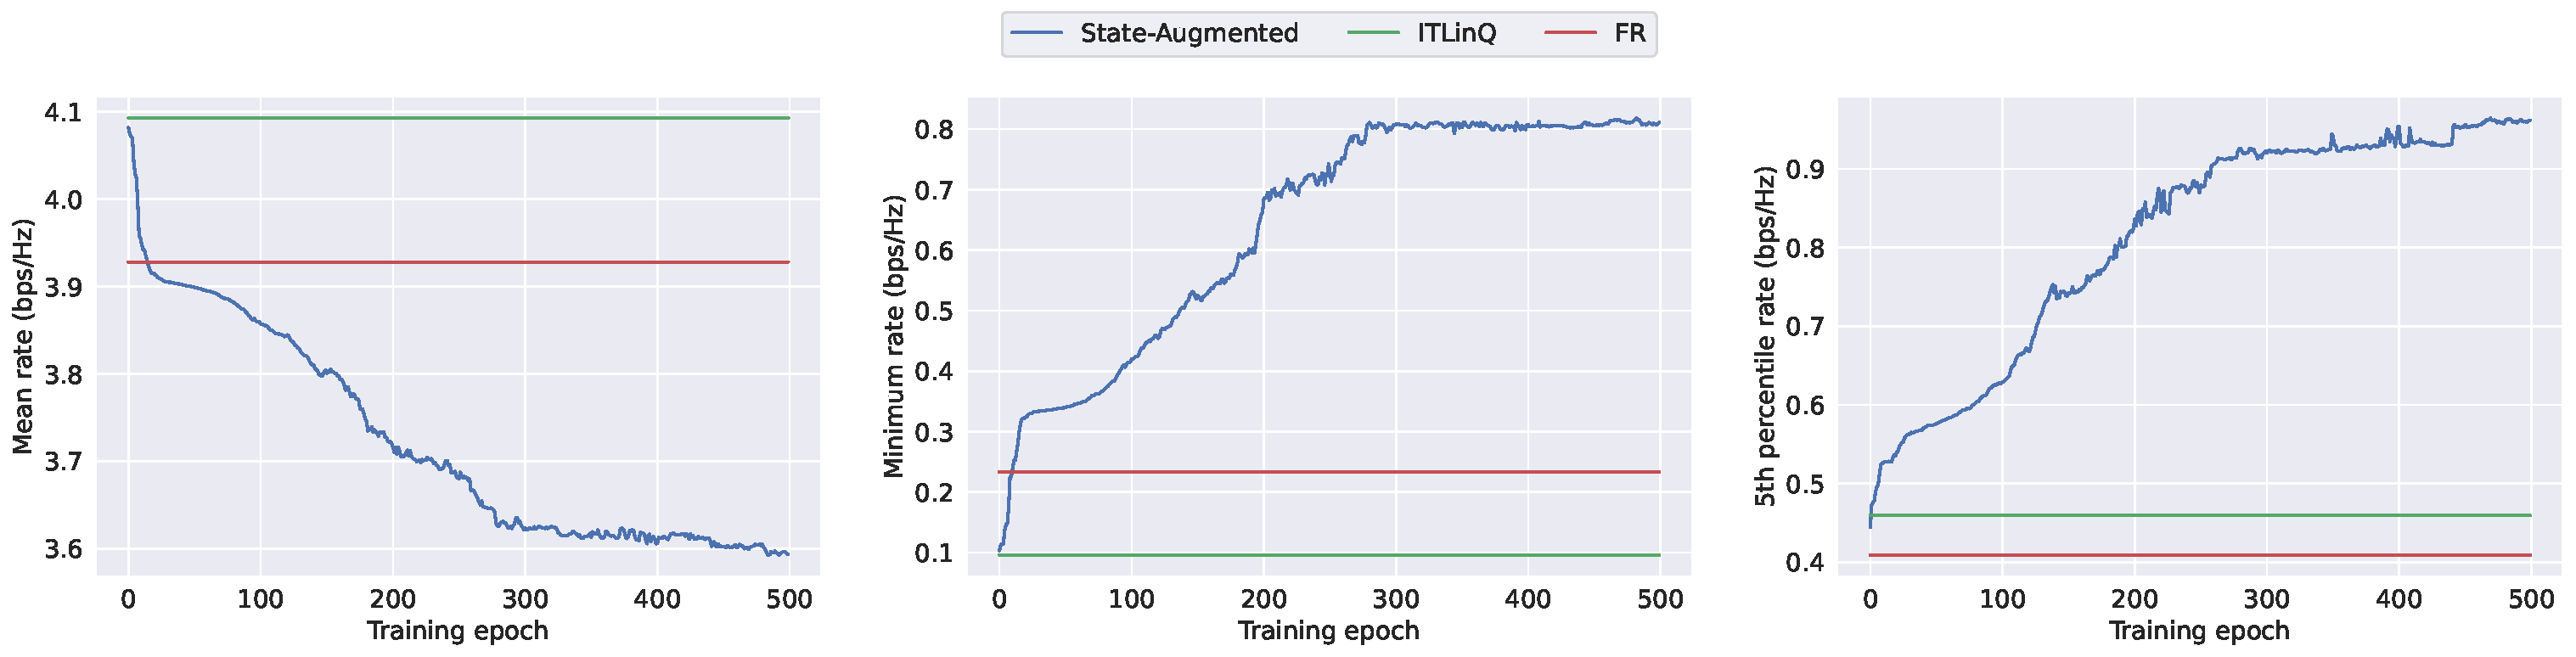
\includegraphics[width=\textwidth]{fig_convergence_singleConfig_m50_vardensity.pdf}
\caption{Convergence behavior of the proposed state-augmented RRM algorithm, and its comparison with the baseline methods for a \emph{single} network realization with $m=50$ transmitter-receiver pairs (variable-density scenario). Note that the baseline algorithms fail to achieve the minimum-rate requirement of $f_{\min}=0.6$, while our proposed method is able to satisfy the constraints for all $50$ users.
}
\label{fig:convergence_singleConfig_m50_vardensity}
\end{figure*}


\begin{figure*}[h]
\centering
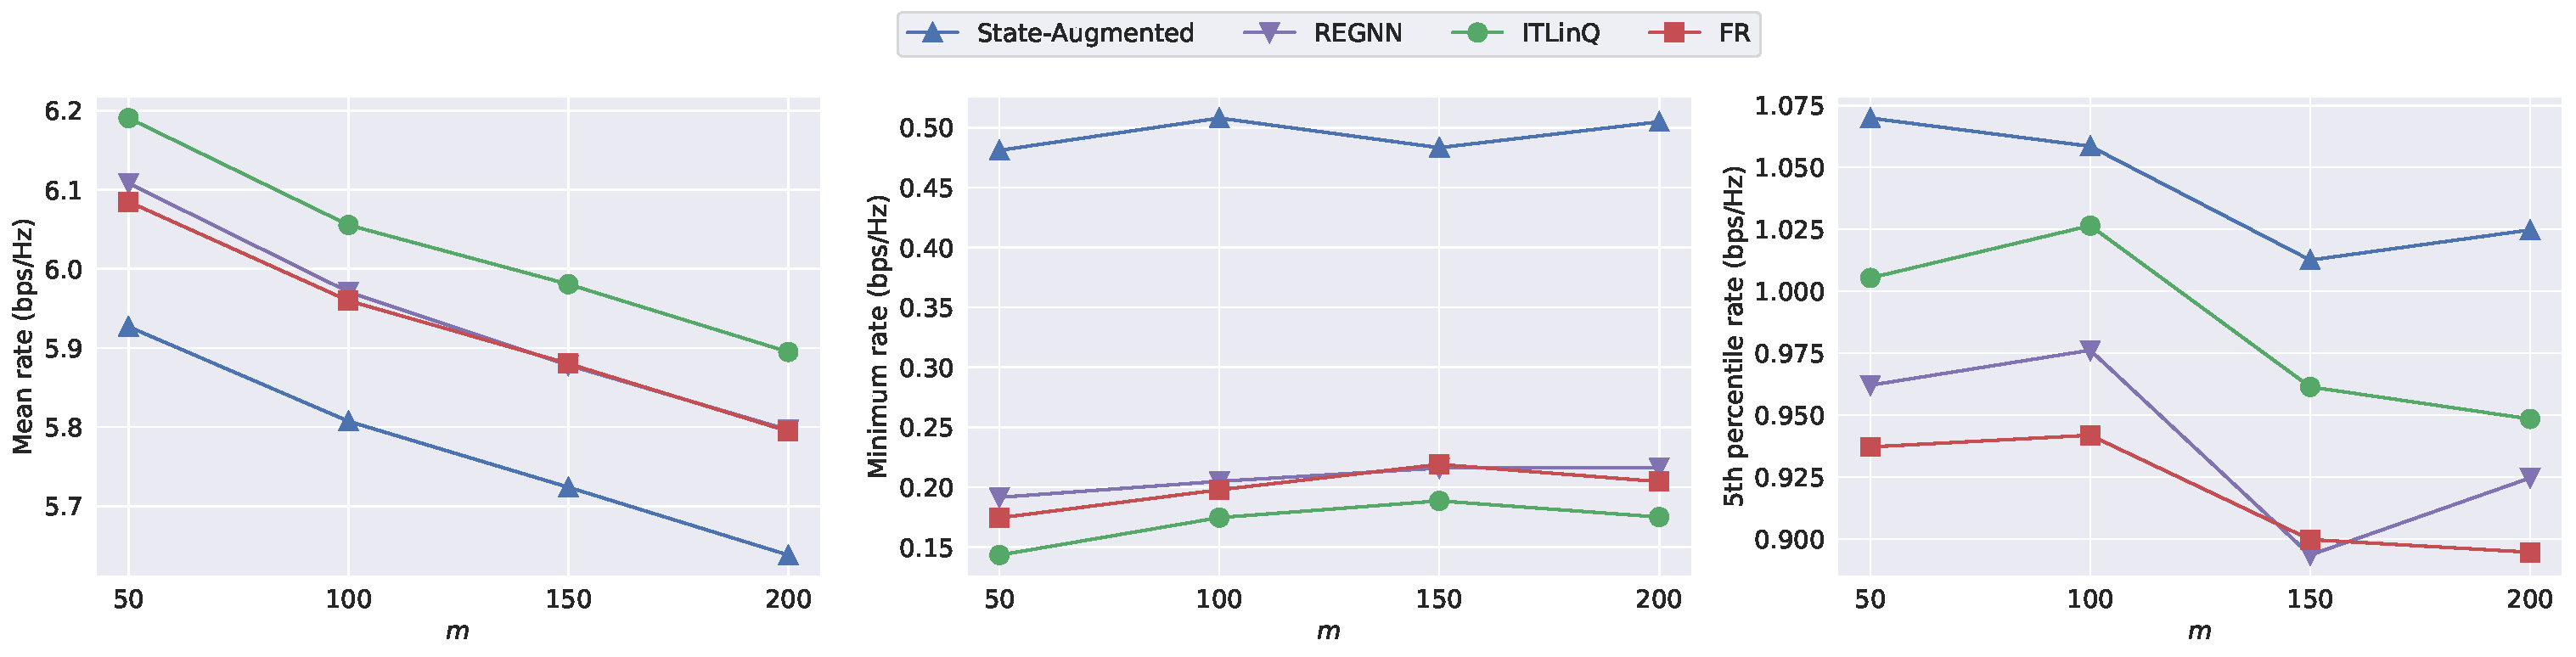
\includegraphics[width=\textwidth]{fig_scalability_fixed_density.pdf}
\caption{Performance comparison of the proposed state-augmented RRM algorithm against baseline methods in the fixed-density scenario for networks with $m\in\{50,100,150,200\}$ transmitter-receiver pairs.}
\label{fig:scalability_fixed_density}
\end{figure*}

\subsection{Experimental Results}\label{sec:exp_results}
We generate networks with $m$ transmitter-receiver pairs, located randomly within a square network area of side length $R$. We drop the transmitters uniformly at random within the network area, while ensuring a minimum distance of $75$m between each pair of them. Afterwards, for each transmitter, we drop its associated receiver uniformly at random within an annulus around the transmitter, with inner and outer radii of $10$m and $50$m, respectively. To control the network density, we consider the following two scenarios to determine the network area size:
\begin{itemize}
    \item \textbf{Fixed Density:} We set $R = \sqrt{m / 20} \times 2$km to keep the density constant (at $5$ users/km$^2$).
    \item \textbf{Variable Density:} We set $R=2$km, implying that the network density increases with $m$.
\end{itemize}
In both cases, and for all values of $m$, we set $f_{\min} = 0.6$bps/Hz, $T_0=5$, and $T=100$. We consider both large-scale and small-scale fading for the channel model. The large-scale fading follows a dual-slope path-loss model similar to~\cite{zhang2015downlink,andrews2016we,naderializadeh2022learning} alongside a $7$dB log-normal shadowing. Moreover, the small-scale fading models channel variations across different time steps following a Rayleigh distribution with a pedestrian speed of $1$m/s~\cite{li2002simulation}. We set the maximum transmit power to $P_{\max}=10$dBm, and the noise variance to $N=-104$dBm (due to the $10$MHz bandwidth and noise power spectral density of $-174$dBm/Hz).

We use a $3$-layer GNN with $F_1=F_2=64$, where the first two layers are based on the local extremum operator proposed in~\cite{ranjan2020asap}, while the last layer entails a linear projection (together with the mapping in~\eqref{eq:final_power_levels_GNN}). We set the primal and dual learning rates to $\eta_{\bbphi} = 10^{-1} / m$ and $\eta_{\bbmu} = 20$, respectively, and we set the batch size to $B=128$. For each value of $m$, we generate a total of $256$ training samples and $128$ samples for evaluation, where each sample refers to a realization of the transmitter/receiver locations (and the large-scale fading), alongside the small-scale fading random process. We set the normalization factor for edge weights at time step $t$ to $Z_t = \left\|\log\left(P_{\max}|\bbH_t|^2 / N\right)\right\|_2$. Except for the case of Section~\ref{sec:single_network} below, we run training for $100$ epochs, and we draw the dual variables during training randomly from the $U(0,1)$ distribution.

\urlstyle{tt}
As baselines, we compare the performance of our proposed method against three baselines: i) Full reuse (FR), where every transmitter uses $P_{\max}$; ii) Information-theoretic link scheduling (ITLinQ)~\cite{naderializadeh2014itlinq}, and iii) random-edge graph neural networks (REGNN)~\cite{eisen2020optimal}.\footnote{For a fair comparison with~\cite{eisen2020optimal}, we use the same exact GNN structure and hyperparameters as for our method to implement the REGNN method.} We would like to point out that, while the REGNN baseline allows the consideration of minimum-rate constraints, the first two baselines (i.e., FR and ITLinQ) are not able to handle such per-user requirements. In what follows, we primarily report the results in terms of three separate metrics, namely the mean rate, minimum rate (discarding the bottom 1\% of user rates as outliers), and the 5\textsuperscript{th} percentile rate, evaluated over the test configurations.\footnote{Our code is available at \url{https://github.com/navid-naderi/StateAugmented_RRM_GNN}.}




\begin{figure*}[h]
\centering
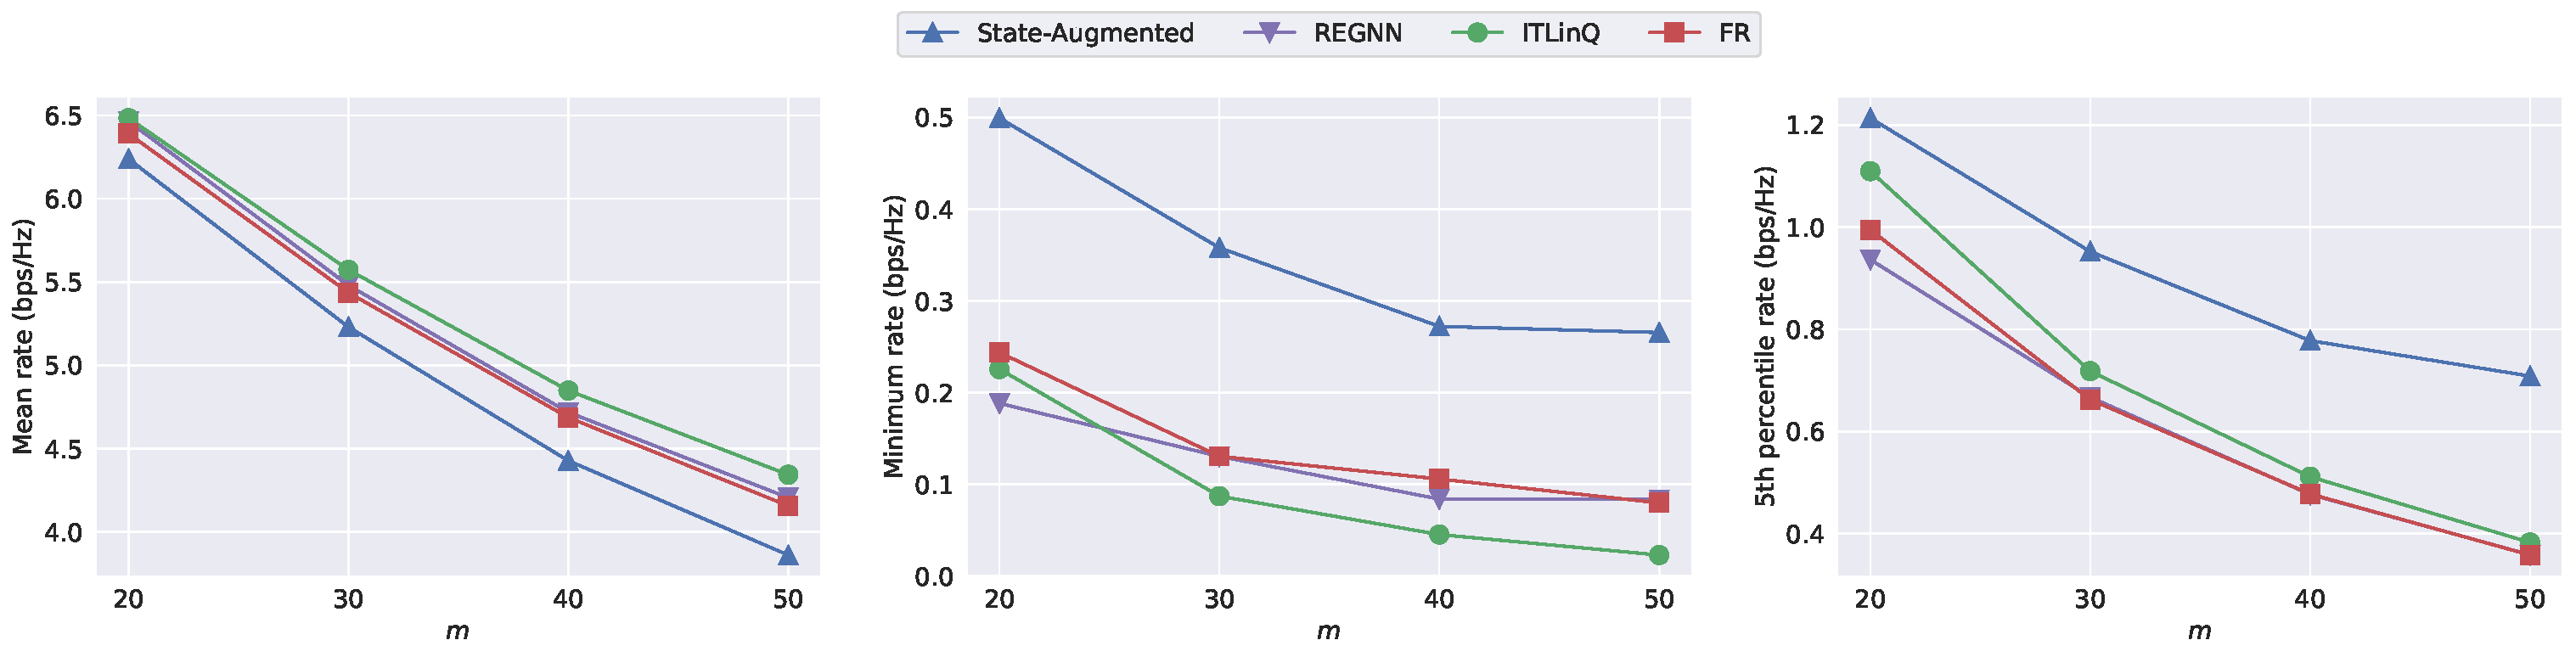
\includegraphics[width=\textwidth]{fig_scalability_variable_density.pdf}
\caption{Performance comparison of the proposed state-augmented RRM algorithm against baseline methods in the variable-density scenario for networks with $m\in\{20, 30, 40, 50\}$ transmitter-receiver pairs.}
\label{fig:scalability_variable_density}
\end{figure*}


\begin{figure*}[t!]
    \centering
    \begin{subfigure}[t]{0.5\textwidth}
        \centering
        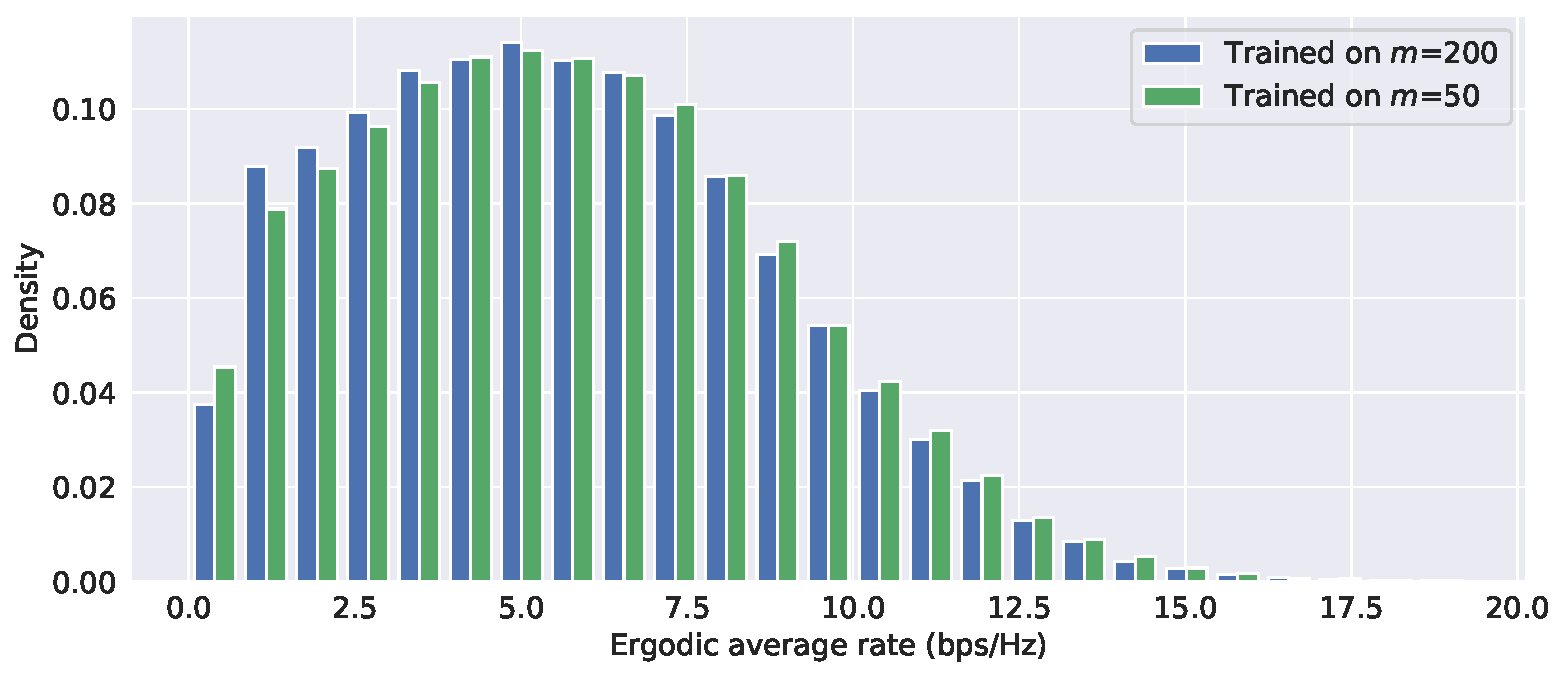
\includegraphics[width=.95\textwidth]{fig_transfer_fixed_density_50To200.pdf}
        \caption{\hspace*{-.25in}}
        \label{fig:transfer_fixed_density_50To200}
    \end{subfigure}%
    \hfill
    \begin{subfigure}[t]{0.5\textwidth}
        \centering
        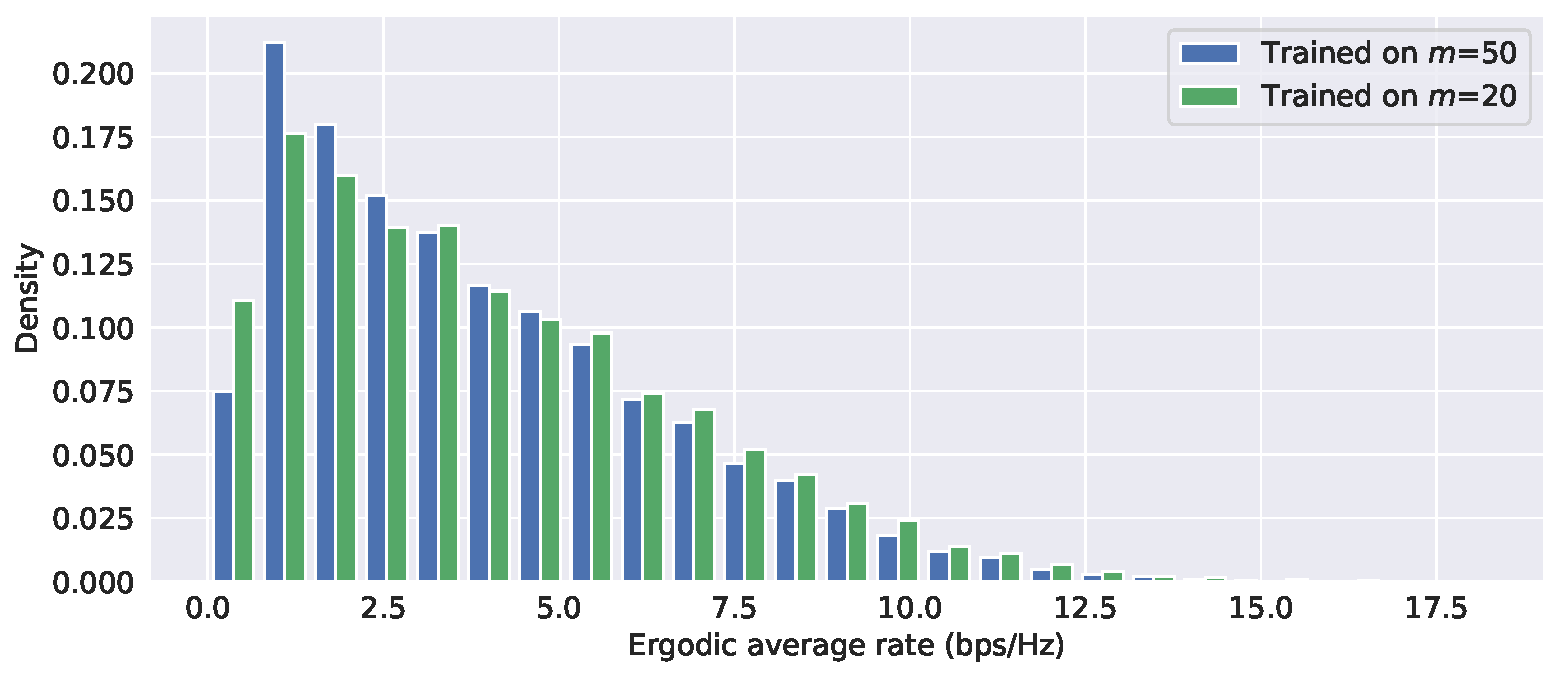
\includegraphics[width=.95\textwidth]{fig_transfer_variable_density_20To50.pdf}
        \caption{\hspace*{-.25in}}
        \label{fig:transfer_variable_density_20To50}
    \end{subfigure}%
    \caption{Transferability of the proposed state-augmented RRM procedure, shown as the histogram of ergodic average rates, for the (a) fixed-density scenario, evaluated on samples with $m=200$, and (b) variable-density scenario, evaluated on samples with $m=50$.}
    \label{fig:transferability}
\end{figure*}

\begin{figure*}[h]
\centering
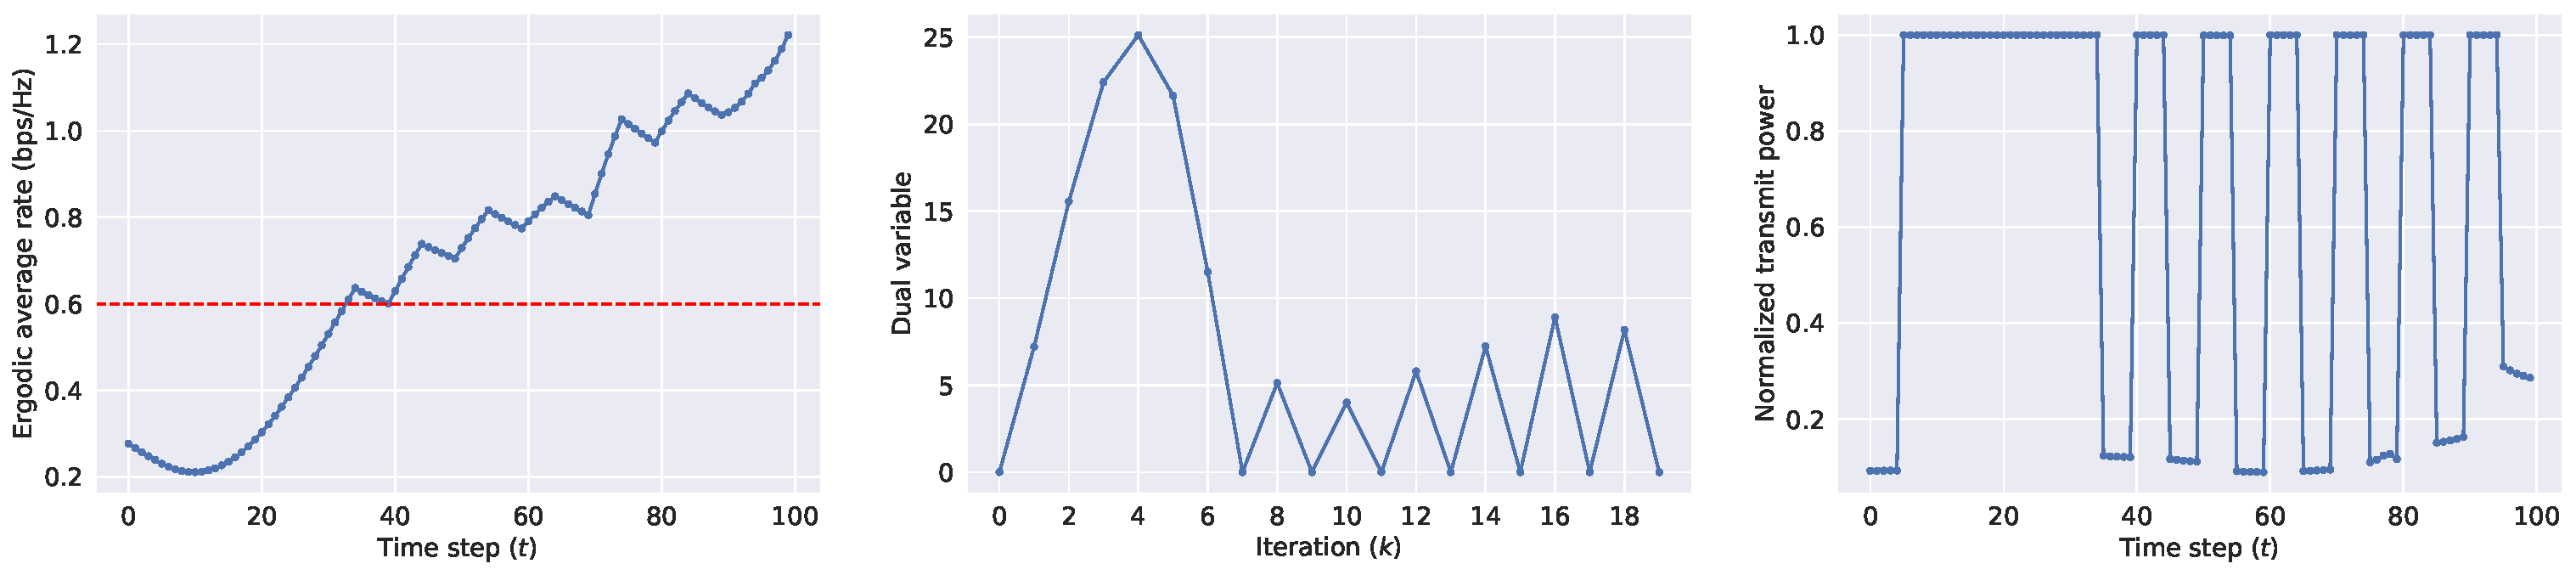
\includegraphics[width=\textwidth]{fig_policy_switching_m50_vardensity.pdf}
\caption{Evolution of the ergodic average rate (left), dual variable (middle), and normalized transmit power level (right) for an example user in a network with $m=50$ transmitter-receiver pairs (for the variable-density scenario). The dashed line in the left plot represents the minimum-rate requirement, i.e., $f_{\min}=0.6$.}
\label{fig:policy_switching_m50_vardensity}
\end{figure*}

\begin{figure}[h]
\centering
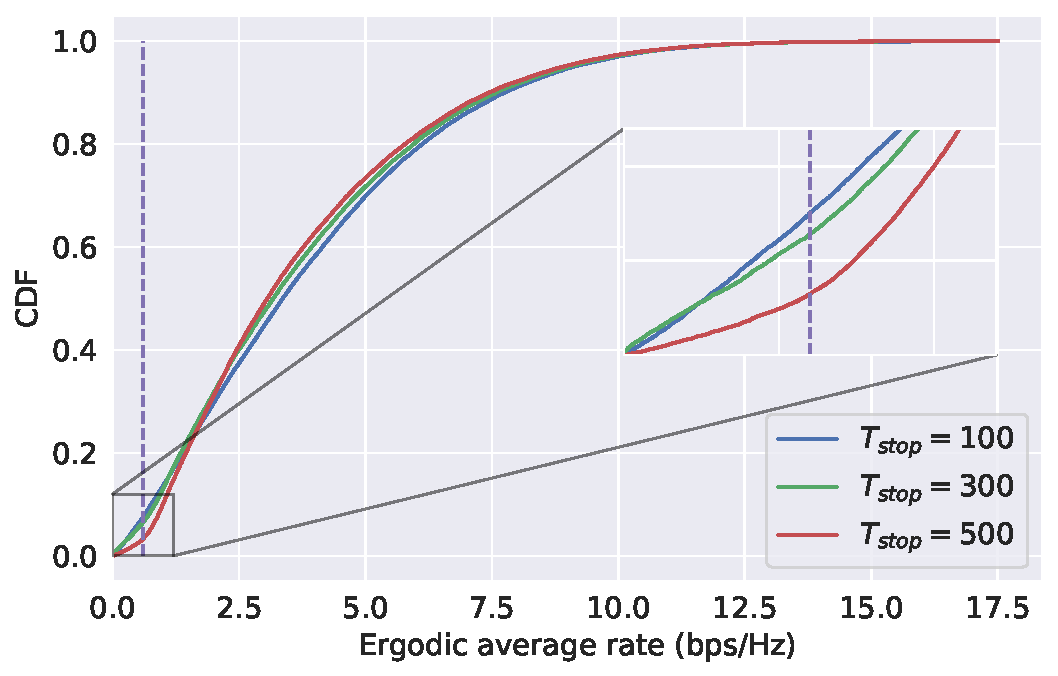
\includegraphics[width=.95\columnwidth]{fig_early_stopping_m50_vardensity_T500.pdf}
\caption{Impact of the early stopping of the dual descent updates on users' ergodic average rates in networks with $m=50$ transmitter-receiver pairs (for the variable-density scenario). The dashed line represents the minimum-rate requirement, i.e., $f_{\min}=0.6$.}
\label{fig:early_stopping_m50_vardensity_T500}
\end{figure}

% \begin{figure*}[h]
% \centering
% \includegraphics[width=\textwidth]{figs/impactoffmin_m6_T0_5.pdf}
% \caption{Impact of the minimum-rate constraint lower bound, $f_{\min}$, on the performance achieved by the proposed state-augmented RRM algorithm in networks with $m=6$ transmitter-receiver pairs (for the variable-density scenario).}
% \label{fig:impactoffmin_m6_T0_5}
% \end{figure*}


\subsubsection{Single Network Realization}\label{sec:single_network}
Figure~\ref{fig:convergence_singleConfig_m50_vardensity} shows the performance of our proposed method against the baselines for a \emph{single} network realization with $m=50$ users (in the variable-density scenario). For this specific experiment, we continue training for $500$ epochs, and decay the primal learning rate by $0.5$ every $100$ epochs. At the end of each training epoch, we evaluate the RRM algorithm on the same realization that is used for training. As the figure shows, our proposed state-augmented RRM algorithm considerably gains over the baseline algorithms in terms of the minimum and 5\textsuperscript{th} percentile rates, managing to satisfy the minimum-rate requirements for all users at the expense of a smaller achieved mean rate.

\subsubsection{Scalability}
Here, we assess the performance of the the proposed algorithm in \emph{families} of networks with different numbers of users, where the policies trained on samples with a specific value of $m$ are evaluated on test samples with the same value of $m$. Figures~\ref{fig:scalability_fixed_density} and~\ref{fig:scalability_variable_density} compare the performance of our proposed method with the baseline algorithms in the fixed-density and variable-density scenarios, respectively. In both scenarios, thanks to the feasibility guarantees of our proposed method for the per-user minimum-rate constraints, our method significantly outperforms the baseline methods in terms of the minimum rate and the 5\textsuperscript{th} percentile rate. This, however, comes at the cost of a slightly lower mean rate. Note that such a scalability is due to the size-invariant property of GNN-based parameterizations (where the number of parameters is fixed regardless of the graph size), as opposed to other parameterizations, such as multi-layer perceptrons (i.e., fully-connected neural networks).

\subsubsection{Transferability to Unseen Network Sizes}
Another upside of the size-invariance property of GNNs is that they can be evaluated on graph sizes not encountered throughout the training process. Figure~\ref{fig:transfer_fixed_density_50To200} shows the histogram of user ergodic average rates under our proposed algorithm in test networks of size $m=200$ (fixed-density scenario) using two GNNs: one trained on samples with $m=200$ and the other trained on samples with $m=50$. Moreover, Figure~\ref{fig:transfer_variable_density_20To50} shows a similar histogram for the variable-density scenario, where GNNs trained on samples with $m=50$ and $m=20$ are evaluated on test samples with $m=50$. As the figures show, in both cases, the trained GNNs provide excellent transferability to larger network sizes, achieving user rates that are similar to the GNNs without the train/test mismatch. Moreover, as expected, the transferred performance is more desirable in the fixed-density scenario than the variable-density scenario, as the channel statistics mostly remain similar in the former case, while in the latter case, the network becomes more interference-limited as $m$ grows.


\subsubsection{Policy Switching}
Figure~\ref{fig:policy_switching_m50_vardensity} shows what an example receiver experiences over the course of the $T=100$ time steps in a test network with $m=50$ transmitter-receiver pairs (for the variable-density scenario) once training is completed. Letting $i$ denote the receiver index, at each time step $t$, we plot its ergodic average rate up to that time step (i.e., $\frac{1}{t} \sum_{\tau=1}^t f_i(\bbH_{\tau}, \bbp(\bbH_{\tau},\bbmu_{\lfloor \tau / T_0 \rfloor};\bbphi^{\star}))$), its dual variable at the corresponding iteration (i.e., $\mu_{i,\lfloor t / T_0 \rfloor}$), and the selected normalized transmit power of transmitter $i$ at that time step (i.e., $p_i(\bbH_t,\bbmu_{\lfloor t / T_0 \rfloor};\bbphi^{\star}) / P_{\max}$). As the figure shows, a \emph{policy switching} behavior occurs, where for the time steps in which the receiver's ergodic average rate is below $f_{\min}$, the dual variable increases, leading to the corresponding transmitter using full transmit power. Moreover, when the ergodic average rate exceeds $f_{\min}$, the transmitter uses an on-off pattern to maintain its receiver's high ergodic average rate, while minimizing the interference caused at other receivers. This shows why state-augmentation is crucial for the algorithm to be able to switch the policy if/when necessary, depending on the constraint violations over time. Indeed, neither the ``off'' policy ($p_i=0$) nor the ``on'' policy ($p_i=P_{\max}$) guarantees the satisfaction of the constraints by itself. However, the illustrated policy switching behavior in Figure~\ref{fig:policy_switching_m50_vardensity} is exactly what the transmitters need to show in order to be able to satisfy their constraints in the long run.

\subsubsection{Drawback of Early Stopping of Dual Descent Iterations}
As we mentioned in Section~\ref{sec:alg}, the feasibility and near-optimality of the RRM decisions depend on the fact that the dual descent iterations in~\eqref{eq:mu_dynamics_augmented} continue for the entire duration of the execution phase. This implies that such feasibility and near-optimality guarantees will not hold if the dual descent updates are stopped at a small, finite number of iterations. Figure~\ref{fig:early_stopping_m50_vardensity_T500} illustrates the empirical cumulative distribution function (CDF) of the user ergodic average rates in test networks with $m=50$ transmitter-receiver pairs (for the variable-density scenario), where the dual descent updates are stopped at a certain time step $T_{\text{stop}} \in \{100, 300, 500\}$. For the sake of this experiment, we expanded the execution time horizon to $T=500$ time steps. As the figure shows, early stopping of the dual variable updates leads to a larger fraction of users violating their minimum-rate requirements. Quite interestingly, such an early stopping provides an equivalent way of implementing the regular primal-dual REGNN method in~\cite{eisen2020optimal}.

\subsubsection{Inference Computational Complexity}
The size-invariance property of the GNNs implies that the number of GNN parameters does not depend on the underlying graph size on which the GNN is operating. However, using GNNs on larger graph sizes naturally leads to a higher computational complexity. Figure~\ref{fig:inference_time_vs_m} shows the average inference time (on CPU) for graphs corresponding to networks with $m\in[20, 200]$ transmitter-receiver pairs. Note that, in practice, the inference time can effectively be reduced by parallelizing computations on GPU hardware architectures.

\begin{figure}[t!]
\centering
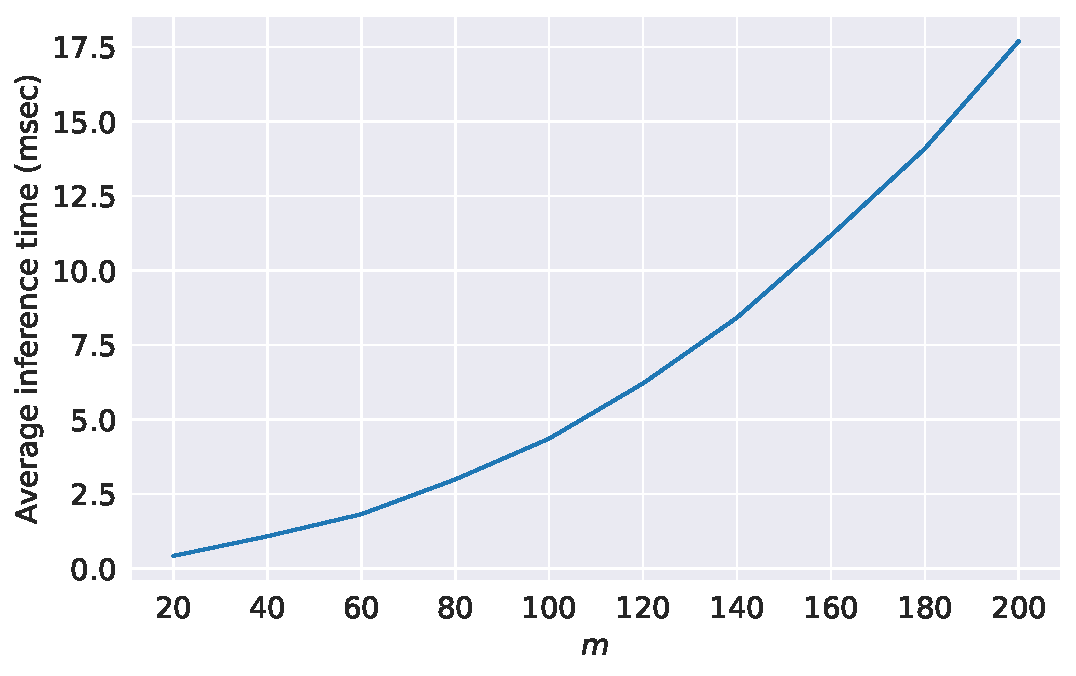
\includegraphics[width=.97\columnwidth]{fig_inference_time_vs_m.pdf}
\caption{Average inference time (on a CPU hardware architecture) for networks with $m\in[20,200]$ transmitter-receiver pairs.}
\label{fig:inference_time_vs_m}
\end{figure}


% \subsubsection{Impact of the Minimum-Rate Constraint Lower Bounds}
% In all our experiments, we set the lower bounds for the minimum-rate constraints, i.e., $f_{\min}$ to $\frac{3}{4}$. This resulted in RRM decisions that attempted to satisfy relatively strict minimum-rate constraints for almost all network realizations, which came at the cost of lower mean rates as compared to baseline methods. Figure~\ref{fig:impactoffmin_m6_T0_5} demonstrates the impact of the constraint lower bounds $f_{\min} \in \left\{\frac{1}{4}, \frac{1}{2}, \frac{3}{4}, 1\right\}$ on the performance of the proposed state-augmented RRM algorithm when trained and evaluated on networks with $m=6$ transmitter-receiver pairs (in the variable-density scenario). As the figure shows, tuning $f_{\min}$ reveals the trade-off between the average and worst-case performance of users across all network realizations. Finding the best minimum-rate constraint lower bound is a non-trivial problem, and it has also been shown that this bound can be tuned adaptively based on each specific network realization through the introduction of learnable slack parameters~\cite{naderializadeh2020wireless, naderializadeh2022learning, naderializadeh2022adaptive}. We leave the incorporation of adaptive minimum-rate constraints into state-augmented RRM algorithms as future work.

\section{Concluding Remarks}\label{sec:conclusion}
We considered the problem of resource allocation in wireless network, termed radio resource management (RRM), in which the goal is to maximize a network-wide utility subject to constraints on the long-term average performance of the network users. We showed how parameterized dual-based RRM policies can lead to feasible and near-optimal solutions, but suffer from multiple challenges, including that they need to be run for an infinite number of time steps and the model parameters have to be optimized for any given set of dual variables at every time step. To mitigate these challenges, we proposed a state-augmented RRM algorithm, which revises the parameterization to take as input the network state, as well as the dual variable at each step, and produce as output the RRM decisions. We showed that for near-universal parameterizations, the proposed method also leads to feasible and near-optimal sequences of RRM decisions. Using graph neural network (GNN) architectures to parameterize the state-augmented RRM policy, we also demonstrated, via a set of numerical experiments, that the proposed method provides scalable and transferable wireless power control solutions that outperform baseline algorithms.




\appendices
\section{Proof of Theorem~\ref{thm:main}}\label{appx:proof}
\allowdisplaybreaks

The arguments used in the proof of Theorem~\ref{thm:main} follow similar steps to those in~\cite{calvo2021state}, with some minor differences specific to our problem formulation, as outlined in Remark~\ref{remark:proof_diff}. We, therefore, include the complete proof here for the paper to be self-complete.% there are differences with prior proofs, specific to our problem formulation, that require us to include the complete proof here.

\subsection{Tightness of The Sequence of Dual Variable Probability Measures}\label{appx:proof_tightness}
We start by proving that the sequence of dual variable probability measures, i.e., $\{p(\bbmu_k|\bbmu_0)\}_{k}$, is tight in the following lemma.

\begin{lemma}
For any $\delta > 0$, there exists a compact set $\ccalA_{\delta}$ such that for every $k \geq 0$, we have $\mathsf{Pr}[\bbmu_k \in \ccalA_{\delta}] > 1 - \delta$.
\end{lemma}

\begin{proof}
Define the dual function, $d(\bbmu)$ as
\begin{align}\label{eq:def_dual_function}
d(\bbmu) = \max_{\bbtheta\in\bbTheta} \ccalL(\bbtheta, \bbmu),
\end{align}
and consider the following set:
\begin{align}\label{eq:def_C}
\ccalC = \left\{\bbmu \in \reals_+^c : d(\bbmu) - P^{\star} \leq \frac{c\eta_{\bbmu}G^2}{2} \right\}.
\end{align}
Now, let
\begin{align}
\ccalA_{\delta} = \ccalB_{\delta} \cup \left(\ccalC \oplus \ccalS_{\sqrt{c\eta_{\bbmu}^2 G^2}}\right),
\end{align}
where $\oplus$ denotes Minkowski sum, $\ccalS_r$ denotes a ball centered at the origin with radius $r\geq0$, and $\ccalB_{\delta}$ is defined as
\begin{align}
\ccalB_{\delta} = \left\{\bbmu \in \reals_+^c : \frac{\| \bbmu - \bbmu^{\star} \|}{\| \bbmu_0 - \bbmu^{\star}\|} \leq \frac{1}{\delta} \right\},
\end{align}
with $\bbmu^{\star}$ representing the optimal set of dual variables. Then, we have
\begin{align}
&\mathsf{Pr}[\bbmu_k \in \ccalA_{\delta}] \nonumber \\
& = \mathsf{Pr}\left[\bbmu_k \in \ccalB_{\delta} \cup \left(\ccalC \oplus \ccalS_{\sqrt{c\eta_{\bbmu}^2 G^2}}\right) \right] \\
& = \underbrace{\mathsf{Pr}\left[\bbmu_k \in \ccalB_{\delta} \cup \left(\ccalC \oplus \ccalS_{\sqrt{c\eta_{\bbmu}^2 G^2}}\right) \middle| \bbmu_{k-1}\in\ccalC \right]}_{\overset{(a)}{=}1} \cdot \ p \nonumber \\
& \quad + \underbrace{\mathsf{Pr}\left[\bbmu_k \in \ccalB_{\delta} \cup \left(\ccalC \oplus \ccalS_{\sqrt{c\eta_{\bbmu}^2 G^2}}\right) \middle| \bbmu_{k-1}\in\ccalC^c \right]}_{\geq \mathsf{Pr}\left[\bbmu_k \in \ccalB_{\delta}  \middle| \bbmu_{k-1}\in\ccalC^c \right]} \cdot \ (1-p) \nonumber \\
& \geq \mathsf{Pr}\left[\bbmu_k \in \ccalB_{\delta}  \middle| \bbmu_{k-1}\in\ccalC^c \right] \\
& = \mathsf{Pr}\left[\frac{\| \bbmu_k - \bbmu^{\star} \|}{\| \bbmu_0 - \bbmu^{\star}\|} \leq \frac{1}{\delta}  \middle| \bbmu_{k-1}\in\ccalC^c \right] \\
& \geq 1 - \left( \frac{\E\left[\| \bbmu_k - \bbmu^{\star} \| \middle| \bbmu_{k-1}\in\ccalC^c\right]}{\| \bbmu_0 - \bbmu^{\star}\|} \right) \delta,
\end{align}
where $p=\mathsf{Pr}\left[\bbmu_{k-1}\in\ccalC \right]$, (a) is true due to the dual dynamics in~\eqref{eq:mu_dynamics} and the fact that the change between $\bbmu_{k-1}$ and $\bbmu_k$ is upper bounded in norm by $\sqrt{c\eta_{\bbmu}^2 G^2}$, and the last inequality is due to conditional Markov's inequality. Therefore, to complete the proof, it suffices to show that (i)
\begin{align}\label{eq:bounded_conditional_difference_norm_muk}
\E\left[\| \bbmu_k - \bbmu^{\star} \| \middle| \bbmu_{k-1}\in\ccalC^c\right] < \| \bbmu_0 - \bbmu^{\star}\|,
\end{align}
and (ii) that $\ccalA_{\delta}$ is compact.

\noindent\textbf{Proof of~\eqref{eq:bounded_conditional_difference_norm_muk}.}
Let $\Delta_{\bbmu_{k-1}}$ be defined as
\begin{align}
\Delta_{\bbmu_{k-1}} \coloneqq \bbg\left( \frac{1}{T_0} \sum_{t=(k-1)T_0}^{kT_0-1} \bbf(\bbH_{t}, \bbp(\bbH_{t};\bbtheta_{k-1})) \right).
\end{align}
Then, from the dual dynamics in~\eqref{eq:mu_dynamics}, we have
\begin{align*}
&\|\bbmu_{k} - \bbmu^{\star}\|^2 \\
&\leq \|\bbmu_{k-1} - \bbmu^{\star} - \eta_{\bbmu} \Delta_{\bbmu_{k-1}} \|^2 \\
&= \|\bbmu_{k-1} - \bbmu^{\star}  \|^2 + \eta_{\bbmu}^2 \|\Delta_{\bbmu_{k-1}} \|^2 \nonumber \\
&\quad - 2\eta_{\bbmu} (\bbmu_{k-1} - \bbmu^{\star})^T \Delta_{\bbmu_{k-1}} \\
&\leq \|\bbmu_{k-1} - \bbmu^{\star}  \|^2 + c \eta_{\bbmu}^2 G^2 - 2\eta_{\bbmu} (\bbmu_{k-1} - \bbmu^{\star})^T \Delta_{\bbmu_{k-1}},
\end{align*}
where the last inequality follows from the fact that for any $i\in\{1,\dots,c\}$, we assume $|g_i\left(\cdot\right)|\leq G$. Taking the expectation of both sides conditioned on $\bbmu_{k-1}$, we have
\begin{align}
&\E\left[\|\bbmu_{k} - \bbmu^{\star}\|^2 \middle| \bbmu_{k-1}\right] \nonumber\\
&\leq \|\bbmu_{k-1} - \bbmu^{\star}  \|^2 + c \eta_{\bbmu}^2 G^2 \nonumber \\
&\quad - 2\eta_{\bbmu} (\bbmu_{k-1} - \bbmu^{\star})^T \E\left[\Delta_{\bbmu_{k-1}}\middle| \bbmu_{k-1}\right]\\
&\leq \|\bbmu_{k-1} - \bbmu^{\star}  \|^2 + c \eta_{\bbmu}^2 G^2 - 2\eta_{\bbmu} (d(\bbmu_{k-1}) - d(\bbmu^{\star}))\label{eq:subgradient}\\
&= \|\bbmu_{k-1} - \bbmu^{\star}  \|^2 + c \eta_{\bbmu}^2 G^2 - 2\eta_{\bbmu} (d(\bbmu_{k-1}) - P^{\star}),\label{eq:pre_C_bound}
\end{align}
where~\eqref{eq:subgradient} follows from the fact that $\Delta_{\bbmu_{k-1}}$ is a subgradient of the dual function~\cite{danskin2012theory}, leading to the inequality $(\bbmu_{k-1} - \bbmu^{\star})^T \E\left[\Delta_{\bbmu_{k-1}}\middle| \bbmu_{k-1}\right] \geq d(\bbmu_{k-1}) - d(\bbmu^{\star})$ thanks to the dual function being convex~\cite{boyd2004convex}. Now, combining the fact that $\bbmu_{k-1}\in\ccalC^c$ with the definition of $\ccalC$ in~\eqref{eq:def_C}, we can continue~\eqref{eq:pre_C_bound} as
\begin{align}
\E\left[\|\bbmu_{k} - \bbmu^{\star}\|^2 \middle| \bbmu_{k-1}\in\ccalC^c\right]
&< \|\bbmu_{k-1} - \bbmu^{\star}\|^2 \\
&< \|\bbmu_{0} - \bbmu^{\star}\|^2,
\end{align}
with the last inequality following from recursion.


\noindent\textbf{Proof of Compactness of $\ccalA_{\delta}$.} Since the Minkowski sum of two compact sets is compact, and also the union of two compact sets is compact, it suffices to show that the set $\ccalC$ is compact.

Given the definition of the dual function in~\eqref{eq:def_dual_function}, for any set of model parameters $\bbtheta\in\bbTheta$ and any set of dual variables $\bbmu\in\reals_+^c$, we have
\begin{align}
d(\bbmu) &\geq \mathcal{U}\left( \frac{1}{T} \sum_{t=0}^{T-1} \bbf(\bbH_t, \bbp(\bbH_t;\bbtheta)) \right)\nonumber \\
   &\qquad\qquad+ \bbmu^T \bbg\left( \frac{1}{T} \sum_{t=0}^{T-1} \bbf(\bbH_t, \bbp(\bbH_t;\bbtheta)) \right)
\end{align}
Now, replacing $\bbtheta$ with the strictly-feasible set of model parameters $\hat{\bbtheta}$ considered in Theorem~\ref{thm:main}, we can write
\begin{align}
d(\bbmu) &\geq \mathcal{U}\left( \frac{1}{T} \sum_{t=0}^{T-1} \bbf(\bbH_t, \bbp(\bbH_t;\hat{\bbtheta})) \right)\nonumber \\
   &\qquad\qquad+ \bbmu^T \bbg\left( \frac{1}{T} \sum_{t=0}^{T-1} \bbf(\bbH_t, \bbp(\bbH_t;\hat{\bbtheta})) \right)\\
&\geq \mathcal{U}\left( \frac{1}{T} \sum_{t=0}^{T-1} \bbf(\bbH_t, \bbp(\bbH_t;\hat{\bbtheta})) \right) + G' \| \bbmu \|_1.\label{eq:dual_upper_bound}
\end{align}
Now, for any $\bbmu\in\ccalC$, according to the definition in~\eqref{eq:def_C}, the bound in~\eqref{eq:dual_upper_bound} leads to
\begin{align}
P^{\star} + \frac{c\eta_{\bbmu}G^2}{2}  \geq \mathcal{U}\left( \frac{1}{T} \sum_{t=0}^{T-1} \bbf(\bbH_t, \bbp(\bbH_t;\hat{\bbtheta})) \right) + G' \| \bbmu \|_1,
\end{align}
implying that $\bbmu$ belongs to the following ball,
\begin{align}
\| \bbmu \|_1 \leq \frac{P^{\star} + \frac{c\eta_{\bbmu}G^2}{2} - \mathcal{U}\left( \frac{1}{T} \sum_{t=0}^{T-1} \bbf(\bbH_t, \bbp(\bbH_t;\hat{\bbtheta})) \right)}{G'},
\end{align}
hence completing the proof.


\end{proof}

\subsection{Proof of Feasibility in~\eqref{eq:thm_feasibility}}\label{appx:proof_feasibility}

From the dual dynamics in~\eqref{eq:mu_dynamics}, we have
\begin{align}\label{eq:mu_inequality}
% \bbmu_{T+1} &\geq \bbmu_T - \eta_{\bbmu} \bbg\left(  \bbf(\bbH_T, \bbp(\bbH_T;\bbtheta_T)) \right).
\bbmu_{K} &\geq \bbmu_{K-1} - \eta_{\bbmu} \bbg\left( \frac{1}{T_0} \sum_{t=(K-1)T_0}^{KT_0-1} \bbf(\bbH_{t}, \bbp(\bbH_{t};\bbtheta_{K-1})) \right)\hspace{-3pt}.
\end{align}
Using the inequality in~\eqref{eq:mu_inequality} recursively yields
% \begin{align}
% \bbmu_{T+1} &\geq \bbmu_1 - \eta_{\bbmu} \sum_{t=1}^T \bbg\left(  \bbf(\bbH_t, \bbp(\bbH_t;\bbtheta_t)) \right) \\
% &= \bbmu_1 - T \eta_{\bbmu} \left(\frac{1}{T} \sum_{t=1}^T  \bbg\left(  \bbf(\bbH_t, \bbp(\bbH_t;\bbtheta_t)) \right)\right) \\
% &\geq \bbmu_1 - T \eta_{\bbmu}  \bbg\left( \frac{1}{T} \sum_{t=1}^T  \bbf(\bbH_t, \bbp(\bbH_t;\bbtheta_t)) \right),
% \end{align}
\begin{align*}
&\bbmu_{K} \nonumber \\
&\geq \bbmu_0 - \eta_{\bbmu} \sum_{k=0}^{K-1} \bbg\left( \frac{1}{T_0} \sum_{t=kT_0}^{(k+1)T_0-1} \bbf(\bbH_{t}, \bbp(\bbH_{t};\bbtheta_k)) \right) \nonumber \\
&= \bbmu_0 - K\eta_{\bbmu} \cdot \frac{1}{K}\hspace{-3pt}\sum_{k=0}^{K-1} \bbg\left( \frac{1}{T_0} \sum_{t=kT_0}^{(k+1)T_0-1} \bbf(\bbH_{t}, \bbp(\bbH_{t};\bbtheta_k)) \right) \nonumber \\
&\geq \bbmu_0 - K\eta_{\bbmu} \bbg\left( \frac{1}{KT_0} \sum_{t=0}^{KT_0-1} \bbf(\bbH_t, \bbp(\bbH_t;\bbtheta_{\lfloor t/T_0 \rfloor})) \right),
\end{align*}
where the last inequality follows from the concavity of $\bbg(\cdot)$. Therefore, we have
% \begin{align}\label{eq:muT+1_vs_mu1}
% &\limsup_{T\to\infty}\bbmu_{T+1}  \nonumber\\ 
% &\geq \bbmu_1 - \eta_{\bbmu} \liminf_{T\to\infty} T \bbg\left( \frac{1}{T} \sum_{t=1}^T  \bbf(\bbH_t, \bbp(\bbH_t;\bbtheta_t)) \right).
% \end{align}
\begin{align}\label{eq:muT+1_vs_mu1}
&\limsup_{K\to\infty}\bbmu_{K+1}  \nonumber\\ 
&\geq \bbmu_0 - \eta_{\bbmu} \liminf_{K\to\infty} K \bbg\left( \frac{1}{T} \sum_{t=0}^{T-1} \bbf(\bbH_t, \bbp(\bbH_t;\bbtheta_{\lfloor t/T_0 \rfloor})) \right).
\end{align}
Now, assume by contradiction that one of the constraints in~\eqref{eq:thm_feasibility} is not satisfied. More precisely, assume there exists an index $i\in\{1,\dots,c\}$ and positive constants $\delta>0$ and $\beta\in(0,1)$ such that
\begin{align}\label{eq:contradiction_prob}
\mathsf{Pr}\left[\liminf_{T\to\infty} g_i\left( \frac{1}{T} \sum_{t=0}^{T-1} \bbf(\bbH_t, \bbp(\bbH_t;\bbtheta_{\lfloor t/T_0 \rfloor})) \right) \leq -\delta \right] = \beta.
\end{align}
This implies that with non-zero probability $\beta$, we would have
% \begin{align}
% &\limsup_{T\to\infty} \|\bbmu_{T+1}\|_1 \nonumber \\
% &\geq \limsup_{T\to\infty} \mu_{i,T+1}\label{eq:1_norm} \\
% &\geq \mu_{i,1} - \eta_{\bbmu} \liminf_{T\to\infty} T g_i\left( \frac{1}{T} \sum_{t=1}^T  \bbf(\bbH_t, \bbp(\bbH_t;\bbtheta_t)) \right)\label{eq:ith_bound} \\
% &\geq \mu_{i,1} + \eta_{\bbmu} \liminf_{T\to\infty} T \epsilon \label{eq:contradiction_prob_use} \\
% &= \infty,
% \end{align}
\begin{align}
&\limsup_{K\to\infty} \|\bbmu_{K}\|_1 \nonumber \\
&\geq \limsup_{K\to\infty} \mu_{i,K}\label{eq:1_norm} \\
&\geq \mu_{i,0} - \eta_{\bbmu} \liminf_{K\to\infty} K g_i\left( \frac{1}{T} \sum_{t=0}^{T-1} \bbf(\bbH_t, \bbp(\bbH_t;\bbtheta_{\lfloor t/T_0 \rfloor})) \right)\label{eq:ith_bound} \\
&\geq \mu_{i,0} + \eta_{\bbmu} \liminf_{K\to\infty} K \epsilon \label{eq:contradiction_prob_use} \\
&= \infty,
\end{align}
where~\eqref{eq:1_norm} follows from the definition of the $\ell_1$-norm% and the fact that $\mu_{i,T+1} \geq 0$
,~\eqref{eq:ith_bound} follows from the $i$\textsuperscript{th} inequality in~\eqref{eq:muT+1_vs_mu1}, and~\eqref{eq:contradiction_prob_use} follows from~\eqref{eq:contradiction_prob}. This contradicts the fact that the sequence of dual variable probabilities is tight, hence completing the proof.
\hfill$\square$


\subsection{Proof of Optimality in~\eqref{eq:thm_optimality}}


Given the dual dynamics in~\eqref{eq:mu_dynamics} and the fact that projection onto the non-negative orthant does not increase the $\ell_2$-norm, we have
\begin{align}
&\left\|\bbmu_{K+1}\right\|^2\nonumber\\
&\leq \left\|\bbmu_K - \eta_{\bbmu} \bbg\left( \frac{1}{T_0} \sum_{t=KT_0}^{(K+1)T_0-1} \bbf(\bbH_{t}, \bbp(\bbH_{t};\bbtheta_K)) \right) \right\|^2\label{eq:norm_dual_update}\\
&=\left\|\bbmu_K \right\|^2 + \eta_{\bbmu}^2 \left\| \bbg\left( \frac{1}{T_0} \sum_{t=KT_0}^{(K+1)T_0-1} \bbf(\bbH_{t}, \bbp(\bbH_{t};\bbtheta_K)) \right)\right\|^2 \nonumber \\
&~\quad- 2\eta_{\bbmu}\bbmu_K^T \bbg\left( \frac{1}{T_0} \sum_{t=KT_0}^{(K+1)T_0-1} \bbf(\bbH_{t}, \bbp(\bbH_{t};\bbtheta_K)) \right)\label{eq:norm_dual_square_expansion}\\
&\leq\left\|\bbmu_T\right\|^2 + c\eta_{\bbmu}^2 G^2  \nonumber \\
&~\quad - 2\eta_{\bbmu}\bbmu_K^T \bbg\left( \frac{1}{T_0} \sum_{t=KT_0}^{(K+1)T_0-1} \bbf(\bbH_{t}, \bbp(\bbH_{t};\bbtheta_K)) \right),\label{eq:g_bounded}
\end{align}
% Since $\left\|\bbmu_{T+1}\right\|^2 \geq 0$, expanding the squared norm on the right-hand side of~\eqref{eq:norm_dual_update} yields
% \begin{align}\label{eq:norm_dual_square_expansion}
% 0 &\leq \left\|\bbmu_T\right\|^2 + \eta_{\bbmu}^2 \left\| \bbg\left(  \bbf(\bbH_T, \bbp(\bbH_T, \bbmu_T;\bbtheta)) \right)\right\|^2 - 2\eta_{\bbmu}\bbmu_T^T \bbg\left(  \bbf(\bbH_T, \bbp(\bbH_T, \bbmu_T;\bbtheta)) \right) .
% \end{align}
%Since 
where the last inequality follows from the fact that for any $i\in\{1,\dots,c\}$, we assume $|g_i\left(\cdot\right)|\leq G$. Applying~\eqref{eq:g_bounded} recursively yields
\begin{align}
&\left\|\bbmu_{K+1}\right\|^2 \nonumber\\
&\leq \left\|\bbmu_0\right\|^2 + c\eta_{\bbmu}^2 K G^2  \nonumber \\
&~\quad - 2\eta_{\bbmu} \sum_{k=0}^{K-1} \bbmu_k^T \bbg\left( \frac{1}{T_0} \sum_{t=kT_0}^{(k+1)T_0-1} \bbf(\bbH_{t}, \bbp(\bbH_{t};\bbtheta_k)) \right).\label{eq:g_bounded_recursive}
\end{align}
Since $\left\|\bbmu_{K+1}\right\|^2 \geq 0$, rearranging the terms in~\eqref{eq:g_bounded_recursive} and normalizing both sides by $2\eta_{\bbmu}K$ results in
% \begin{align}\label{eq:inner_prod_dual_init}
% \bbmu_T^T \bbg\left(  \bbf(\bbH_T, \bbp(\bbH_T, \bbmu_T;\bbtheta)) \right) \leq \frac{1}{2\eta_{\bbmu}}\left\|\bbmu_T\right\|^2 + \frac{c\eta_{\bbmu}G^2}{2}.
% \end{align}
% Applying~\eqref{eq:inner_prod_dual_init} recursively and normalizing by $T$, we will have
\begin{align}\label{eq:inner_prod_dual_recursive_normalized}
&\frac{1}{K} \sum_{k=0}^{K-1} \bbmu_k^T \bbg\left( \frac{1}{T_0} \sum_{t=kT_0}^{(k+1)T_0-1} \bbf(\bbH_{t}, \bbp(\bbH_{t};\bbtheta_k)) \right)\nonumber \\
&\leq \frac{1}{2\eta_{\bbmu}K} \left\|\bbmu_0\right\|^2 + \frac{c\eta_{\bbmu}G^2}{2}.
\end{align}
Taking the conditional expectation of both sides in~\eqref{eq:inner_prod_dual_recursive_normalized} given $\bbmu_0$, and letting $K\to\infty$, we can write
\begin{align}
&\limsup_{K\to\infty} \E\left[\sum_{k=0}^{K-1} \frac{\bbmu_k^T}{K} \bbg\left(  \sum_{t=kT_0}^{(k+1)T_0-1} \frac{\bbf(\bbH_{t}, \bbp(\bbH_{t};\bbtheta_k))}{T_0} \right)\middle|\bbmu_0\right] \nonumber \\
&\leq \frac{c\eta_{\bbmu}G^2}{2}.\label{eq:inner_prod_dual_limsup}
\end{align}


%%%% SINGLE-STEP MU UPDATES
% Given the dual dynamics in~\eqref{eq:mu_dynamics} and the fact that projection onto the non-negative orthant does not increase the $\ell_2$-norm, we have
% \begin{align}
% \left\|\bbmu_{T+1}\right\|^2 &\leq \left\|\bbmu_T - \eta_{\bbmu} \bbg\left(  \bbf(\bbH_T, \bbp(\bbH_T;\bbtheta_{\lfloor T / T_0 \rfloor})) \right)\right\|^2\label{eq:norm_dual_update}\\
% &=\left\|\bbmu_T\right\|^2 + \eta_{\bbmu}^2 \left\| \bbg\left(  \bbf(\bbH_T, \bbp(\bbH_T;\bbtheta_{\lfloor T / T_0 \rfloor})) \right)\right\|^2 \nonumber \\
% &~\quad- 2\eta_{\bbmu}\bbmu_T^T \bbg\left(  \bbf(\bbH_T, \bbp(\bbH_T;\bbtheta_{\lfloor T / T_0 \rfloor})) \right)\label{eq:norm_dual_square_expansion}\\
% &\leq\left\|\bbmu_T\right\|^2 + c\eta_{\bbmu}^2 G^2  \nonumber \\
% &~\quad - 2\eta_{\bbmu}\bbmu_T^T \bbg\left(  \bbf(\bbH_T, \bbp(\bbH_T;\bbtheta_{\lfloor T / T_0 \rfloor})) \right),\label{eq:g_bounded}
% \end{align}
% % Since $\left\|\bbmu_{T+1}\right\|^2 \geq 0$, expanding the squared norm on the right-hand side of~\eqref{eq:norm_dual_update} yields
% % \begin{align}\label{eq:norm_dual_square_expansion}
% % 0 &\leq \left\|\bbmu_T\right\|^2 + \eta_{\bbmu}^2 \left\| \bbg\left(  \bbf(\bbH_T, \bbp(\bbH_T, \bbmu_T;\bbtheta)) \right)\right\|^2 - 2\eta_{\bbmu}\bbmu_T^T \bbg\left(  \bbf(\bbH_T, \bbp(\bbH_T, \bbmu_T;\bbtheta)) \right) .
% % \end{align}
% %Since 
% where the last inequality follows from the fact that for any $k\in\{1,\dots,c\}$, we assume $|g_k\left(  \bbf(\bbH_T, \bbp(\bbH_T;\bbtheta_{\lfloor T / T_0 \rfloor}))\right)|\leq G$. Applying~\eqref{eq:g_bounded} recursively yields
% \begin{align}
% \left\|\bbmu_{T+1}\right\|^2 &\leq \left\|\bbmu_1\right\|^2 + c\eta_{\bbmu}^2 T G^2  \nonumber \\
% &~\quad - 2\eta_{\bbmu} \sum_{t=1}^T \bbmu_t^T \bbg\left(  \bbf(\bbH_t, \bbp(\bbH_t;\bbtheta_{\lfloor t / T_0 \rfloor})) \right).\label{eq:g_bounded_recursive}
% \end{align}
% Since $\left\|\bbmu_{T+1}\right\|^2 \geq 0$, rearranging the terms in~\eqref{eq:g_bounded_recursive} and normalizing both sides by $2\eta_{\bbmu}T$ results in
% % \begin{align}\label{eq:inner_prod_dual_init}
% % \bbmu_T^T \bbg\left(  \bbf(\bbH_T, \bbp(\bbH_T, \bbmu_T;\bbtheta)) \right) \leq \frac{1}{2\eta_{\bbmu}}\left\|\bbmu_T\right\|^2 + \frac{c\eta_{\bbmu}G^2}{2}.
% % \end{align}
% % Applying~\eqref{eq:inner_prod_dual_init} recursively and normalizing by $T$, we will have
% \begin{align}\label{eq:inner_prod_dual_recursive_normalized}
% \frac{1}{T} \sum_{t=1}^T \bbmu_t^T \bbg\left(  \bbf(\bbH_t, \bbp(\bbH_t;\bbtheta_{\lfloor t / T_0 \rfloor})) \right) \leq \frac{1}{2\eta_{\bbmu}T} \left\|\bbmu_1\right\|^2 + \frac{c\eta_{\bbmu}G^2}{2}.
% \end{align}
% Taking the conditional expectation of both sides in~\eqref{eq:inner_prod_dual_recursive_normalized} given $\bbmu_1$, and letting $T\to\infty$, we can write
% \begin{align}\label{eq:inner_prod_dual_limsup}
% \limsup_{T\to\infty}\frac{1}{T} \sum_{t=1}^T \E\left[\bbmu_t^T \bbg\left(  \bbf(\bbH_t, \bbp(\bbH_t;\bbtheta_{\lfloor t / T_0 \rfloor})) \right) | \bbmu_1 \right] \leq \frac{c\eta_{\bbmu}G^2}{2}.
% \end{align}



% {\color{black} %\textbf{Alternative solution:}

For any iteration $k$, since $\bbtheta_k$ is the maximizer of~\eqref{eq:theta_dynamics}, for any $\bbtheta\in\bbTheta$, we can write
\begin{align}
& \mathcal{U}\left( \frac{1}{T_0} \sum_{t=kT_0}^{(k+1)T_0-1} \bbf(\bbH_{t}, \bbp(\bbH_{t};\bbtheta_k)) \right)\nonumber \\
   &\qquad+ \bbmu_{k}^T \bbg\left( \frac{1}{T_0} \sum_{t=kT_0}^{(k+1)T_0-1} \bbf(\bbH_{t}, \bbp(\bbH_{t};\bbtheta_k)) \right)\nonumber   \\
& \geq \mathcal{U}\left( \frac{1}{T_0} \sum_{t=kT_0}^{(k+1)T_0-1} \bbf(\bbH_{t}, \bbp(\bbH_{t};\bbtheta)) \right)\nonumber \\
   &\qquad+ \bbmu_{k}^T \bbg\left( \frac{1}{T_0} \sum_{t=kT_0}^{(k+1)T_0-1} \bbf(\bbH_{t}, \bbp(\bbH_{t};\bbtheta)) \right)\nonumber 
\end{align}

Taking the expectations of both sides conditioned on $\bbmu_{k}$, we have
\begin{align}
&\E\left[\mathcal{U}\left( \frac{1}{T_0} \sum_{t=kT_0}^{(k+1)T_0-1} \bbf(\bbH_{t}, \bbp(\bbH_{t};\bbtheta_k)) \right)\middle| \bbmu_{k} \right]\nonumber \\
   &\qquad+ \bbmu_{k}^T \E\left[\bbg\left( \frac{1}{T_0} \sum_{t=kT_0}^{(k+1)T_0-1} \bbf(\bbH_{t}, \bbp(\bbH_{t};\bbtheta_k)) \right)\middle| \bbmu_{k} \right]\nonumber   \\
&\geq \E\left[\mathcal{U}\left( \frac{1}{T_0} \sum_{t=kT_0}^{(k+1)T_0-1} \bbf(\bbH_{t}, \bbp(\bbH_{t};\bbtheta)) \right)\right]\nonumber \\
   &\qquad+ \bbmu_{k}^T \E\left[\bbg\left( \frac{1}{T_0} \sum_{t=kT_0}^{(k+1)T_0-1} \bbf(\bbH_{t}, \bbp(\bbH_{t};\bbtheta)) \right)\right] \\
&= \E\left[\mathcal{U}\left( \frac{1}{T_0} \sum_{t=kT_0}^{(k+1)T_0-1} \bbf(\bbH_{t}, \bbp(\bbH_{t};\bbtheta)) \right)\right]\nonumber \\
   &\qquad+ \underbrace{\bbmu_{k}^T}_{\geq 0} \underbrace{\E\left[\bbg\left( \frac{1}{T_0} \sum_{t=kT_0}^{(k+1)T_0-1} \bbf(\bbH_{t}, \bbp(\bbH_{t};\bbtheta)) \right)\right]}_{\geq 0 \text{ for any feasible }\bbtheta\in\bbTheta}\label{eq:unbiased_estimate_prev_exp}\\
&= \lim_{T\to\infty} \mathcal{U}\left( \frac{1}{T} \sum_{t=0}^{T-1} \bbf(\bbH_t, \bbp(\bbH_t;\bbtheta)) \right)\nonumber \\
   &\qquad+ \underbrace{\bbmu_{k}^T}_{\geq 0} \lim_{T\to\infty} \underbrace{\bbg\left( \frac{1}{T} \sum_{t=0}^{T-1} \bbf(\bbH_t, \bbp(\bbH_t;\bbtheta)) \right)}_{\geq 0 \text{ for any feasible }\bbtheta\in\bbTheta}\label{eq:unbiased_estimate_Ug_Tinf}\\
& \geq \lim_{T\to\infty} \mathcal{U}\left( \frac{1}{T} \sum_{t=0}^{T-1} \bbf(\bbH_t, \bbp(\bbH_t;\bbtheta)) \right), \label{eq:objective_RHS}
\end{align}
where~\eqref{eq:unbiased_estimate_Ug_Tinf} follows from the fact that the expected value of the utility and the constraints within each iteration provide unbiased estimates of the objective and constraints in~\eqref{eq:param_problem}, respectively; i.e., for any $k\in\{0,1,2,\dots,K-1\}$ and $\forall \bbtheta \in \bbTheta$,
\begin{align}
&\E\left[\mathcal{U}\left( \frac{1}{T_0} \sum_{t=kT_0}^{(k+1)T_0-1} \bbf(\bbH_{t}, \bbp(\bbH_{t};\bbtheta)) \right)\right] \nonumber \\
&\qquad\qquad\qquad = \lim_{T\to\infty}\mathcal{U}\left( \frac{1}{T} \sum_{t=0}^{T-1} \bbf(\bbH_t, \bbp(\bbH_t;\bbtheta)) \right) \\
&\E\left[\bbg\left( \frac{1}{T_0} \sum_{t=kT_0}^{(k+1)T_0-1} \bbf(\bbH_{t}, \bbp(\bbH_{t};\bbtheta)) \right)\right] \nonumber \\
&\qquad\qquad\qquad = \lim_{T\to\infty}\bbg\left( \frac{1}{T} \sum_{t=0}^{T-1} \bbf(\bbH_t, \bbp(\bbH_t;\bbtheta)) \right).
\end{align}
The inequality in~\eqref{eq:objective_RHS} is true for all feasible $\bbtheta\in\bbTheta$, especially for the optimal set of parameters $\bbtheta^{\star}$, for which the RHS of~\eqref{eq:objective_RHS} equals $P^{\star}$. Therefore, we have
\begin{align}
&\E\left[\mathcal{U}\left( \frac{1}{T_0} \sum_{t=kT_0}^{(k+1)T_0-1} \bbf(\bbH_{t}, \bbp(\bbH_{t};\bbtheta_k)) \right)\middle| \bbmu_{k} \right]\nonumber \\
&\geq P^{\star} - \bbmu_{k}^T \E\left[\bbg\left( \frac{1}{T_0} \sum_{t=kT_0}^{(k+1)T_0-1} \bbf(\bbH_{t}, \bbp(\bbH_{t};\bbtheta_k)) \right)\middle| \bbmu_{k} \right].
% &\geq P^{\star} - \lim_{T\to\infty} \bbmu_t^T \bbg\left( \frac{1}{T} \sum_{t'=t}^{t+T-1} \E\left[\bbf(\bbH_{t'}, \bbp(\bbH_{t'};\bbtheta_t)) | \bbmu_t\right] \right) \\
% &\geq P^{\star} - \lim_{T\to\infty} \bbmu_t^T \bbg\left( \frac{1}{T} \sum_{t'=KT}^{t+T-1} \E\left[\bbf(\bbH_{t'}, \bbp(\bbH_{t'};\bbtheta_t)) | \bbmu_t\right] \right) \\
% &= P^{\star} - \lim_{T\to\infty} \bbmu_t^T \bbg\left( \E\left[\bbf(\bbH_{t}, \bbp(\bbH_{t};\bbtheta_t))| \bbmu_t\right] \right) \nn{?}
\end{align}
Averaging the above inequality over $k\in\{0,\dots,K-1\}$, and taking the expected value conditioned on $\bbmu_0$, we will get
\begin{align}
&\E\Bigg[\frac{1}{K} \sum_{k=0}^{K-1} \mathcal{U}\left( \frac{1}{T_0} \sum_{t=kT_0}^{(k+1)T_0-1} \bbf(\bbH_{t}, \bbp(\bbH_{t};\bbtheta_k)) \right)\Bigg| \bbmu_{0} \Bigg]\nonumber \\
&\geq P^{\star} \nonumber \\
& -\E\Bigg[\frac{1}{K} \sum_{k=0}^{K-1} \bbmu_{k}^T \bbg\left( \frac{1}{T_0} \sum_{t=kT_0}^{(k+1)T_0-1} \bbf(\bbH_{t}, \bbp(\bbH_{t};\bbtheta_k)) \right)\Bigg| \bbmu_{0} \Bigg]\hspace{-1pt}.\label{eq:avg_K_ineq}
\end{align}
Letting $K\to\infty$, and plugging~\eqref{eq:inner_prod_dual_limsup} into~\eqref{eq:avg_K_ineq}, we have
\begin{align}
& P^{\star} - \frac{c\eta_{\mu}G^2}{2} \nonumber \\
&\leq P^{\star} \nonumber \\
& - \limsup_{K\to\infty} \E\left[\sum_{k=0}^{K-1} \frac{\bbmu_k^T}{K} \bbg\left(  \sum_{t=kT_0}^{(k+1)T_0-1} \tfrac{\bbf(\bbH_{t}, \bbp(\bbH_{t};\bbtheta_k))}{T_0} \right)\middle|\bbmu_0\right] \\
&\leq \liminf_{K\to\infty} \E\Bigg[\frac{1}{K}\hspace{-2pt} \sum_{k=0}^{K-1} \mathcal{U}\left( \frac{1}{T_0} \sum_{t=kT_0}^{(k+1)T_0-1} \bbf(\bbH_{t}, \bbp(\bbH_{t};\bbtheta_k)) \right) \Bigg] \\
&\leq \liminf_{K\to\infty} \E\Bigg[ \mathcal{U}\left( \frac{1}{K}\hspace{-2pt} \sum_{k=0}^{K-1} \frac{1}{T_0} \sum_{t=kT_0}^{(k+1)T_0-1} \bbf(\bbH_{t}, \bbp(\bbH_{t};\bbtheta_k)) \right) \Bigg] \label{eq:U_concavity}\\
&= \liminf_{T\to\infty} \E\Bigg[ \mathcal{U}\left( \frac{1}{T} \sum_{t=0}^{T-1} \bbf(\bbH_{t}, \bbp(\bbH_{t};\bbtheta_{\lfloor t / T_0 \rfloor})) \right) \Bigg] \label{eq:final_optimality}
\end{align}
where~\eqref{eq:U_concavity} is due to concavity of $\mathcal{U}$. This completes the proof, due to the assumption that the limit on the left-hand side of~\eqref{eq:final_optimality} exists.
\hfill$\square$

\begin{remark}\label{remark:proof_diff}
Note that the differences between our proof and that of~\cite{calvo2021state} are two-fold: i) In our work, the updates for the dual variables are based on unbiased gradient estimates in~\eqref{eq:unbiased_estimate_prev_exp} as opposed to the reinforcement learning scenario in~\cite{calvo2021state}; and ii) The time averaging operation in our problem formulation happens inside the utility and constraint functions, $\ccalU$ and $\bbg$, respectively, as opposed to the formulation in~\cite{calvo2021state}, where the time averaging operation happens outside the reward functions.
\end{remark}



% \begin{align}
% &P^{\star} - \frac{1}{K} \sum_{t=K}^T \E\left[\bbmu_t^T \bbg\left( \frac{1}{T} \sum_{t'=t}^{t+T-1} \E\left[\bbf(\bbH_{t'}, \bbp(\bbH_{t'};\bbtheta_t)) | \bbmu_t\right] \right) \bigg| \bbmu_1\right] \nonumber\\
% % &P^{\star} - \lim_{T\to\infty} \frac{1}{T} \sum_{t=1}^T \E\left[\bbmu_t^T \bbg\left( \E\left[\bbf(\bbH_{t}, \bbp(\bbH_{t};\bbtheta_t))| \bbmu_t\right] \right)| \bbmu_1\right] \nonumber\\
% &\leq \lim_{T\to\infty} \frac{1}{T} \sum_{t=1}^T \E\Bigg[\mathcal{U}\left( \frac{1}{T} \sum_{t'=t}^{t+T-1} \bbf(\bbH_{t'}, \bbp(\bbH_{t'};\bbtheta_t)) \right)\Bigg| \bbmu_1\Bigg] \\
% &\leq \lim_{T\to\infty} \E\Bigg[\mathcal{U}\left( \frac{1}{T^2} \sum_{t=1}^T \sum_{t'=t}^{t+T-1} \bbf(\bbH_{t'}, \bbp(\bbH_{t'};\bbtheta_t)) \right)\Bigg| \bbmu_1\Bigg] 
% \end{align}


% }


% PREV SOLUTION USING DUAL FUNCTION CONVEXITY
% \pagebreak


% Now, define the dual function, $d(\bbmu)$ as
% \begin{align}
% d(\bbmu) = \max_{\bbtheta\in\bbTheta} \ccalL(\bbtheta, \bbmu).
% \end{align}
% Then, given the fact that the dual function is convex, we have
% \begin{align}
% \frac{1}{T} \sum_{t=1}^T d(\bbmu_t) &\geq d\left(\frac{1}{T} \sum_{t=1}^T \bbmu_t\right) \\
% &\geq P^{\star},\label{eq:dual_larger_primal}
% \end{align}
% where~\eqref{eq:dual_larger_primal} follows from the fact that the dual function upper bounds the value of the primal for any set of dual variables $\bbmu\in\reals_+^c$. 
% Now, for any Lagrangian-maximizing set of parameters $\bbtheta_t$, we can write the dual function $d(\bbmu_t)$ as
% \begin{align}
% d(\bbmu_t) &= \mathcal{U}\left( \frac{1}{T} \sum_{t'=1}^T \bbf(\bbH_{t'}, \bbp(\bbH_{t'};\bbtheta_t)) \right) \nonumber \\
% &\quad+ \bbmu_t^T \bbg\left( \frac{1}{T} \sum_{t'=1}^T \bbf(\bbH_{t'}, \bbp(\bbH_{t'};\bbtheta_t)) \right)\label{eq:dual_mut} %\\
% % &= \E\left[\mathcal{U}\left(  \bbf(\bbH_t, \bbp(\bbH_t;\bbtheta)) \right)\right] \nonumber \\
% % &\quad+ \E\left[\bbmu_t^T \bbg\left(  \bbf(\bbH_t, \bbp(\bbH_t;\bbtheta)) \right)\right].\label{eq:dual_mut}
% \end{align}

% \begin{align}
% \E[d(\bbmu_t)] &= \E\left[\mathcal{U}\left( \frac{1}{T} \sum_{t'=t+1}^{t+T} \bbf(\bbH_{t'}, \bbp(\bbH_{t'};\bbtheta_t)) \right) | \bbmu_t\right] \nonumber \\
% &\quad+ \E\left[\bbmu_t^T \bbg\left( \frac{1}{T} \sum_{t'=t+1}^{t+T} \bbf(\bbH_{t'}, \bbp(\bbH_{t'};\bbtheta_t)) \right)| \bbmu_t\right]\\
% &\leq \E\left[\mathcal{U}\left( \frac{1}{T} \sum_{t'=t+1}^{t+T} \bbf(\bbH_{t'}, \bbp(\bbH_{t'};\bbtheta_t)) \right) | \bbmu_t\right] \nonumber \\
% &\quad+ \bbmu_t^T \bbg\left(\E\left[ \frac{1}{T} \sum_{t'=t+1}^{t+T} \bbf(\bbH_{t'}, \bbp(\bbH_{t'};\bbtheta_t)) | \bbmu_t\right]\right)
% \end{align}
% Combining~\eqref{eq:dual_mut} and~\eqref{eq:dual_larger_primal}, we have
% \begin{align}
% & \E\left[\mathcal{U}\left( \frac{1}{T^2} \sum_{t=1}^T\sum_{t'=1}^T \bbf(\bbH_{t'}, \bbp(\bbH_{t'};\bbtheta_t)) \right)\right] \nonumber\\
% &\geq \frac{1}{T} \sum_{t=1}^T \E\left[\mathcal{U}\left( \frac{1}{T} \sum_{t'=1}^T \bbf(\bbH_{t'}, \bbp(\bbH_{t'};\bbtheta_t)) \right)\right] \nonumber\\
% &\geq P^{\star} - \frac{1}{T} \sum_{t=1}^T \E\left[\bbmu_t^T \bbg\left( \frac{1}{T} \sum_{t'=1}^T \bbf(\bbH_{t'}, \bbp(\bbH_{t'};\bbtheta_t)) \right)\right].
% \end{align}
% % \begin{align}
% % &\frac{1}{T} \sum_{t=1}^T \E\left[\mathcal{U}\left(  \bbf(\bbH_t, \bbp(\bbH_t, \bbmu_t;\bbtheta)) \right)\right] \nonumber\\
% % &\geq P^{\star} - \frac{1}{T} \sum_{t=1}^T \E\left[\bbmu_t^T \bbg\left( \bbf(\bbH_t, \bbp(\bbH_t, \bbmu_t;\bbtheta)) \right)\right].
% % \end{align}
% % Letting $T\to\infty$, we will have
% % \begin{align}
% % &\liminf_{T\to\infty}\frac{1}{T} \sum_{t=1}^T \E\left[\mathcal{U}\left(  \bbf(\bbH_t, \bbp(\bbH_t, \bbmu_t;\bbtheta)) \right)\right] \nonumber \\
% % &\geq P^{\star} - \limsup_{T\to\infty}\frac{1}{T} \sum_{t=1}^T \E\left[\bbmu_t^T \bbg\left( \bbf(\bbH_t, \bbp(\bbH_t, \bbmu_t;\bbtheta)) \right)\right] \nonumber \\
% % &\geq P^{\star} - \frac{c\eta_{\bbmu}G^2}{2},\label{eq:almost_final_optimality}
% % \end{align}
% % where the last inequality results from~\eqref{eq:inner_prod_dual_limsup}. Combining~\eqref{eq:almost_final_optimality} with the fact that $\mathcal{U}(\cdot)$ is concave, we can write
% % \begin{align}
% % &\liminf_{T\to\infty} \E\left[ \mathcal{U}\left( \frac{1}{T} \sum_{t=1}^T \bbf(\bbH_t, \bbp(\bbH_t, \bbmu_t;\bbtheta)) \right)\right] \nonumber \\
% % &\geq \liminf_{T\to\infty} \E\left[ \frac{1}{T} \sum_{t=1}^T \mathcal{U}\left(  \bbf(\bbH_t, \bbp(\bbH_t, \bbmu_t;\bbtheta)) \right)\right] \nonumber \\
% % &= \liminf_{T\to\infty}\frac{1}{T} \sum_{t=1}^T \E\left[\mathcal{U}\left(  \bbf(\bbH_t, \bbp(\bbH_t, \bbmu_t;\bbtheta)) \right)\right] \nonumber \\
% % &\geq P^{\star} - \frac{c\eta_{\bbmu}G^2}{2},\label{eq:final_optimality}
% % \end{align}
% This completes the proof, due to the assumption that the limit on the left-hand side of~\eqref{eq:final_optimality} exists.
%

% \pagebreak

% \balance



\section{Convex Hull Relaxation}\label{appx:convex_hull}
Theorem~\ref{thm:main}---as well as Theorem 1 of~\cite{calvo2021state}---demonstrate the convergence of the time average of the primal-dual iterates. This can indeed be shown for any non-convex optimization problem, and it comes from the fact that the primal-dual iterates operate on a \emph{convex hull} relaxation. More precisely, consider the following generic optimization problem:
\begin{subequations}\label{eq:generic_opt}
\begin{alignat}{2}
    &\max_{x} &~& f_0(x),           \\
    &~~~\text{s.t.} &&  f(x) \geq 0,%
\end{alignat}
\end{subequations}
with the Lagrangian $\ccalL(x,\mu) = f_0(x) + \mu f(x)$ for $\mu \in \reals_+$ and the Lagrangian maximizer
\begin{align}\label{eq:L_max_orig}
x^{\star}(\mu) = \arg \max_x \ccalL(x,\mu).
\end{align}
Now, consider a generalized version of~\eqref{eq:generic_opt}, in which the optimization over $x$ is replaced by an optimization over a \emph{measure} $m(x)$, i.e.,
\begin{subequations}\label{eq:generic_opt_measure}
\begin{alignat}{2}
    &\max_{m(x)} &~& \int f_0(x) \, dm(x),           \\
    &~~~\text{s.t.} &&  \int f(x) \, dm(x) \geq 0.%
\end{alignat}
\end{subequations}
The Lagrangian corresponding to~\eqref{eq:generic_opt_measure} is then given by $\ccalL(m(x),\mu) = \int \left(f_0(x) + \mu f(x) \right)  \, dm(x)$ for $\mu \in \reals_+$, with the Lagrangian maximizer
\begin{align}\label{eq:L_max_measure}
m^{\star}(x|\mu) = \arg \max_{m(x)} \ccalL(m(x),\mu).
\end{align}
The Lagrangian maximizing measure in~\eqref{eq:L_max_measure} may not be unique. However, it can be shown that the Lagrangian maximizer in~\eqref{eq:L_max_orig} also corresponds to a Lagrangian maximizing measure in~\eqref{eq:L_max_measure}, or conversely, the set of Lagrangian maximizing measures in~\eqref{eq:L_max_measure} contains a measure that corresponds to the solution of~\eqref{eq:L_max_orig}.


\section{Proof of Theorem~\ref{thm:near_universality_result}}\label{appx:proof_state_augmented}

The proof of feasibility in~\eqref{eq:thm_feasibility_state_augmented} follows similar steps to those in Appendix~\ref{appx:proof_feasibility} and we, therefore, omit it for brevity. As for the near-optimality result in~\eqref{eq:thm_optimality_state_augmented}, we have %we show that the objectives resulting from the state-augmented procedure and  first consider the following lemma.

\begin{align}
&\lim_{T\to\infty} \Bigg| \E \Bigg[ \mathcal{U}\left( \frac{1}{T} \sum_{t=0}^{T-1} \bbf\left(\bbH_t, \bbp\left(\bbH_t, \bbmu_{\lfloor t/T_0 \rfloor}; \bbphi^{\star}\right) \right) \right) \nonumber \\
&\quad\qquad\qquad - \mathcal{U}\left( \frac{1}{T} \sum_{t=0}^{T-1} \bbf(\bbH_t, \bbp(\bbH_t ;\bbtheta_{\lfloor t / T_0 \rfloor})) \right) \Bigg] \Bigg| \\
&\leq \lim_{T\to\infty} \E \ \Bigg| \ \mathcal{U}\left( \frac{1}{T} \sum_{t=0}^{T-1} \bbf\left(\bbH_t, \bbp\left(\bbH_t, \bbmu_{\lfloor t/T_0 \rfloor}; \bbphi^{\star}\right) \right) \right) \nonumber \\
&\quad\qquad\qquad - \mathcal{U}\left( \frac{1}{T} \sum_{t=0}^{T-1} \bbf(\bbH_t, \bbp(\bbH_t ;\bbtheta_{\lfloor t / T_0 \rfloor})) \right) \Bigg| \label{eq:convexity_abs} \\
&\leq \lim_{T\to\infty} \E \ \Bigg\| \ \frac{1}{T} \sum_{t=0}^{T-1} \bigg( \bbf\left(\bbH_t, \bbp\left(\bbH_t, \bbmu_{\lfloor t/T_0 \rfloor}; \bbphi^{\star}\right) \right)  \nonumber \\
&\qquad\qquad\qquad\qquad\quad -  \bbf\left(\bbH_t, \bbp(\bbH_t ;\bbtheta_{\lfloor t / T_0 \rfloor})\right) \bigg) \Bigg\|_{\infty} \label{eq:Lipschitz_U} \\
&\leq  \lim_{T\to\infty} \frac{1}{T} \sum_{t=0}^{T-1} \E \ \Bigg\| \   \bbf\left(\bbH_t, \bbp\left(\bbH_t, \bbmu_{\lfloor t/T_0 \rfloor}; \bbphi^{\star}\right) \right)  \nonumber \\
&\qquad\qquad\qquad\qquad\quad ~ -  \bbf\left(\bbH_t, \bbp(\bbH_t ;\bbtheta_{\lfloor t / T_0 \rfloor})\right) \Bigg\|_{\infty} \label{eq:convexity_infnorm} \\
&\leq M \lim_{T\to\infty} \frac{1}{T} \sum_{t=0}^{T-1} \E \ \Bigg\| \   \bbp\left(\bbH_t, \bbmu_{\lfloor t/T_0 \rfloor}; \bbphi^{\star}\right)  \nonumber \\
&\qquad\qquad\qquad\qquad\qquad\qquad\quad -  \bbp(\bbH_t ;\bbtheta_{\lfloor t / T_0 \rfloor})  \Bigg\|_{\infty} \label{eq:Lipschitz_f} \\
&\leq M \E \left\| \bbp\left(\bbH, \bbmu; \bbphi^{\star}\right) - \bbp(\bbH ;\bbtheta(\bbmu))  \right\|_{\infty} \label{eq:exp_mu} \\
&\leq M \epsilon,\label{eq:universality_proofbound}
\end{align}
where~\eqref{eq:convexity_abs} results from the convexity of the absolute value function,~\eqref{eq:Lipschitz_U} comes from the Lipschitz continuity of the utility $\mathcal{U}$,~\eqref{eq:convexity_infnorm} results from the convexity of the $\ell_{\infty}$ norm,~\eqref{eq:Lipschitz_f} holds because of the the Lipschitz continuity of the performance function $\bbf$,~\eqref{eq:exp_mu} holds since $\{\bbmu_k\}_{k=1}^K$ are assumed to come from the distribution $p_{\bbmu}$, and~\eqref{eq:universality_proofbound} is true due to the near-universality of the parameterization. This, combined with~\eqref{eq:thm_optimality} from Theorem~\ref{thm:main}, completes the proof.
\hfill$\square$%%


\bibliographystyle{IEEEtran}
\bibliography{references}



\vfill

\end{document}




Table \ref{tab:main} shows the overall result of our method and the SoTAs on three benchmark datasets: MSVD-QA, MSRVTT-QA and NExT-QA. Our observations are summarized as follows:

\begin{itemize}[leftmargin=*]
\item Across all three benchmark datasets, the proposed EIGV outperforms SoTA by a distinct margin (+1.2\%$\sim$2.3\%). Such prevailing performance indicates the overall effectiveness of our design, which underpins the theoretical soundness of the equivariant and invariant principles. 

\item Narrowing the inspection to each of the three backbones, EIGV brings each backbone model a sharp gain across all benchmark datasets (+1.3\%$\sim$5.2\%), which evidences its model-agnostic property. 
%
Nevertheless, we notice that the improvements fluctuate across the backbones. As a comparison, on MSVD-QA and MSRVTT-QA benchmarks, EIGV acquires more favorable gains with backbone Co-Mem and HGA than it does with MSPAN. This is because the multi-granularity hierarchy empowers the MSPAN with robustness, especially to questions of the descriptive type. Therefore, it achieves stronger backbone performances on benchmarks that focus on the descriptive question (\ie MSVD-QA and MSRVTT-QA), which, in turn, account for the contribution of EIGV to some extent, thus makes improvement of MSPAN less remarkable.
% However, this advantage can account for the contribution of EIGV to some extent, thus makes the . 
In contrast, when it comes to the causal and temporal question (\ie NExT-QA) where the inherit advantage of MSPAN backbone vanishes,  EIGV shows equivalent improvements on all three backbones (+2.2\%$\sim$3.7\%). 
%
% In contrast, it promotes the Co-Mem --- the most unappreciated baseline to a SoTA level. Apart from the overall improvement, 

\item Comparing the average improvement across different benchmarks, we notice that EIGV achieves the best improvement on MSVD-QA (+2.3\%$\sim$5.2\%) while relatively moderate gains on MSRVTT-QA (+1.3\%$\sim$1.9\%) and NExT-QA (+2.2\%$\sim$3.7\%).
% , even if two datasets share the same question type and similar video length. 
The reason for such discrepancy is that MSVD-QA is relatively small in size,
which constrains the reasoning ability of the backbone models by limiting their exposure to training instances.
As a comparison, MSVD-QA is five-time smaller than MSRVTT-QA in terms of QA pairs (43K vs 243K), and three-time smaller than NExT-QA in terms of video instances (1970 vs 5440).
However, such deficiency caters to the focal point of EIGV that develops better in a less generalized situation, thus leading to more preferable growth on MSVD-QA.
% As a comparison, MSRVTT-QA is five times larger in terms of QA pairs (43K vs 243K), NExT-QA involves three times more videos (1970 vs 5440). 
% This constrains the reasoning ability of the backbone model by limit exposing of training instance, which, in turn, caters to the focal point of EIGV and lead to preferable growth on MSVD-QA. 
\end{itemize}

% Table generated by Excel2LaTeX from sheet 'Sheet1'
\begin{table}[t]
  \centering
  \caption{Evaluation on the effectiveness of sub-modules}
    \resizebox{0.9\linewidth}{!}{
    \begin{tabular}{c|cc|cc}
    \toprule
    \multirow{2}[2]{*}{Ablation} & \multicolumn{2}{c|}{MSVD-QA} & \multicolumn{2}{c}{NExT-QA} \\
          & MSPAN & HGA   & MSPAN & HGA \\
    \midrule
    \midrule
    SoTA Backbone & 40.3  & 36.6  & 50.7  & 50.0 \\
    \midrule
    $+$ Mixup \cite{DBLP:conf/iclr/ZhangCDL18} & 41.0    & 38.3  & 52.0    & 51.8 \\
    $+$ Intervener & 41.5  & 39.6  & 52.5  & 52.7 \\
    \midrule
    $+$ Disruptor & 40.9  & 37.6  & 51.0    & 51.1 \\
    \white{66666} $+$ Disrupt-Q & 40.6  & 37.0    & 50.8  & 51.0 \\
    \white{66666} $+$ Disrupt-V & 40.7  & 37.3  & 51.0    & 50.8 \\
    \midrule
    EIGV & \textbf{42.6} & \textbf{40.8} & \textbf{52.9} & \textbf{53.7} \\
    \bottomrule
    \end{tabular}%
    }
    \vspace{-15pt}
  \label{tab:ablation}%
\end{table}%



\subsection{In-Depth Study (RQ2)}
\vspace{5pt}
\subsubsection{\textbf{What are the effect of EIGV's components?}}

To comprehensively understand the reasoning mechanism of EIGV, we poke its structure with careful scrutiny. Specifically, we explore the effectiveness of the proposed intervener and disruptor by analyzing their performance with different backbones on two benchmarks. We report the corresponding performances in Table \ref{tab:ablation} and summarize our findings as follows:
\begin{itemize}[leftmargin=*]

\vspace{5pt}
\item \noindent \textbf{Effectiveness of Intervener.} \label{exp:intervener}
We first testify the substantial efficacy of the intervener by comparing its permanence ( ``$+$Intervener'' ) to the backbone. This brings constant gains across different settings (+1.2\%$\sim$3\%), which demonstrates the stability of our design. Then, we compare the result of the intervener with the conventional mixup augmentation \cite{DBLP:conf/iclr/ZhangCDL18}, which can be considered as a simplified case of the interventer that only applies the equivariant intervention to the entire training video. The result shows that our design outperforms the conventional mixup in all cases. This manifests that the benefit of invariant intervention is fundamental, and the functionality of invariance and equivariance principle are mutually reinforced.

\vspace{5pt}
\item \noindent \textbf{Effectiveness of Disruptor.} 
We validate the disruptor design by investigating its components --- the substitution on video (``$+$Disrupt-V'') and the permutation on question (``$+$Disrupt-Q''), respectively. 
Albeit moderate, improvement on (``$+$Disrupt-V'') shows that stressing causal scene can benefit visual robustness.
A similar trend also applies to ``$+$Disrupt-Q'' as well, the constant improvement in all settings shows that acknowledging artificial corrosion in ($v,q$) matching can strengthen vision-language alignment, which is in line with the current finding in the cross-model pre-train literature \cite{DBLP:conf/icml/RadfordKHRGASAM21}. 
Furthermore, the overall result on ``$+$Disrupt'' shows that the advancement of ``$+$Disrupt-V'' and ``$+$Disrupt-Q'' can be amplified by further integration. 
\end{itemize}


% Table generated by Excel2LaTeX from sheet 'Sheet1'
\begin{table}[t]
  \centering
  \caption{Study of feature setting. ``APP'' and ``MOT'' denotes using appearance and motion feature individually. }
    \resizebox{0.95\linewidth}{!}{
    \begin{tabular}{cc|cc|cc}
    \toprule
    \multicolumn{2}{c|}{\multirow{2}[2]{*}{Method}} & \multicolumn{2}{c|}{MSVD-QA} & \multicolumn{2}{c}{NExT-QA} \\
    \multicolumn{2}{c|}{} & MSPAN & HGA   & MSPAN & HGA \\
    \midrule
    \midrule
    \multirow{2}[2]{*}{\rot{APP}} & SoTA Backbone & 40.1  & 35.0    & 49.7  & 48.3 \\
          & \white{66666}$+$ EIGV   & \textbf{41.0}    & \textbf{39.5}  & \textbf{52.0}    & \textbf{52.4} \\
    \midrule
    \multirow{2}[2]{*}{\rot{MOT}} & SoTA Backbone & 37.8  & 33.6  & 49.4  & 47.5 \\
          & \white{66666}$+$ EIGV   & \textbf{39.3}  & \textbf{38.5}  & \textbf{51.1}  & \textbf{51.7} \\
    \bottomrule
    \end{tabular}%
    }
  \vspace{-15pt}
  \label{tab:unifeat}%
\end{table}%





\subsubsection{\textbf{What are the effects of different feature settings?}}
To answer this question, we perform uni-feature tests for the visual representation. Concretely, instead of combining the appearance and motion features together and then manipulating them as a whole, we run ablative experiments on each of them solely.  
%
As shown in Table \ref{tab:unifeat}, under all circumstances, EIGV can improve models trained with appearance and motion features in equivalent magnitude, even though the appearance feature is demonstrated to be more visually informative in backbone comparison. This verifies that our improvement is ascribed to both feature modes rather than accessing only one of them.

% Although, as manifested in baseline comparison, appearance feature are more visually informative, EIGV is able to improve APP and MOT in equivalent magnitude under all circumstances. This verifies that our improvement is ascribed to both feature modes rather than accessing only one of them. 
% %
% Such observation also reveals the possibility that EIGV can mitigate the model's overly reliance on appearance feature \cite{DBLP:conf/iccv/JenniJ21} by balancing the feature exploitation to a commensurate rate, so as to avoid overlooking the visual dynamics in motion feature. 



\subsubsection{\textbf{What are the effects of hyper-parameters?}}
Justifying a reliable design requires a sensitivity test on its hyper-parameters. As shown in Figure \ref{fig:neg}, we probe the potency of EIGV by investigating the distribution of the equivariance mixing ratio and the number of negative samples. Our observations are as follows:

\begin{itemize}[leftmargin=*]
\item Figure \ref{fig:neg}a shows how EIGV performs compared to the SoTA backbone and the conventional mixup augmentation. Specifically, we adjust $\alpha$ to vary the distribution that the equivariant mixing ratio $\lambda_0$ draws from, and cross-check the performance of EIGV (``+EIGV'') against its counterparts (``SoTA Backbone'' and ``+HGA'') on two backbone models. Mixup, despite some improvement, its generalization is limited by the choice of the backbone. For MSPAN backbone, even the heavily tuned $\alpha$ fails to make a reasonable improvement. In contrast, EIGV successively outperforms mixup augmentation and backbone methods in every $\alpha$ setting, which recalls our finding in Section \ref{exp:intervener} and justifies the necessity of the environment-invariance principle.      

\item Figure \ref{fig:neg}b demonstrates how the performance of EIGV varies as the number of negative sample increase. We notice that the predictive curves keep rising until $N$ reaches around five, which indicates that EIGV learns distinctive grounding rationale as more negative samples are considered. This is in line with the finding in the contrastive learning community that additional negative pairs bring about more desirable outcome \cite{he2019moco}. 
%However, we also observe a slight drop as $N$ keep growing large than 5, which since the overwhelming of simple negative sample might compromise the contribution of hard negative and turn to a uniformity if the contrastive temperature $\tau$ is not carefully tuned [], 
\end{itemize}



\subsection{Quantitative Study (RQ3)}
By nature, EIGV is equipped with intrinsic visual interpretability. To capture the learning insight of EIGV, we inspect the predictive answer of some video instances along with their grounded interpretations and show the visualization in Figure \ref{fig:case-study}, where each row provides a video instance and two questions that emphasize the visual content in different temporal spans. Notably, even for the same video instance, EIGV is able to accredit different scenes for the different questions. Nonetheless, we also observe the insufficient grounding result in Row 3 Q1, where the grounding result partially covers the dog swimming scene, while the whole video is answerable to the question.


\begin{figure}[t]
\centering
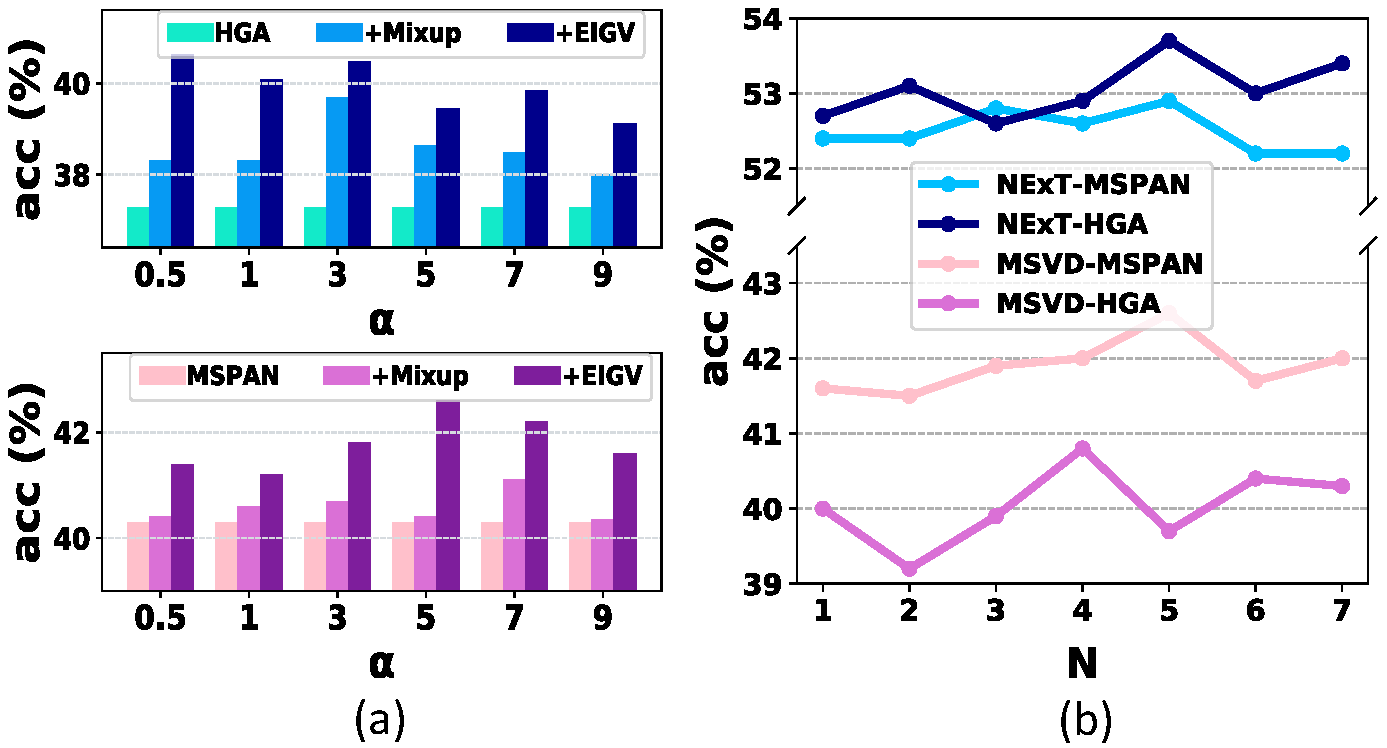
\includegraphics[scale=0.35]{fig/fig5.pdf}
\vspace{-10pt}
\caption{Hyperparameter analysis. (a) Study of $\alpha$ on MSVD-QA, which controls the equivariant mixing ratio by $\lambda_0\sim\text{Beta}(\alpha,\alpha)$. Performance of two EIGV enhanced models --- HGA (top) and MSPAN (bottom) are reported, alongside the SoTA backbone and mixup augmented performances.  
(b) Study on the impact of the negative sample number N, where EIGV with two backbones (\ie MSPAN and HGA) on two benchmark datasets (NExT-QA and MSVD-QA) are reported.}
\vspace{-10pt}
\label{fig:neg}
\end{figure}
\section{Related Work}
\label{sec:related}

\begin{figure*}[t]
  \centering
%   \setlength{\abovecaptionskip}{0.cm}
  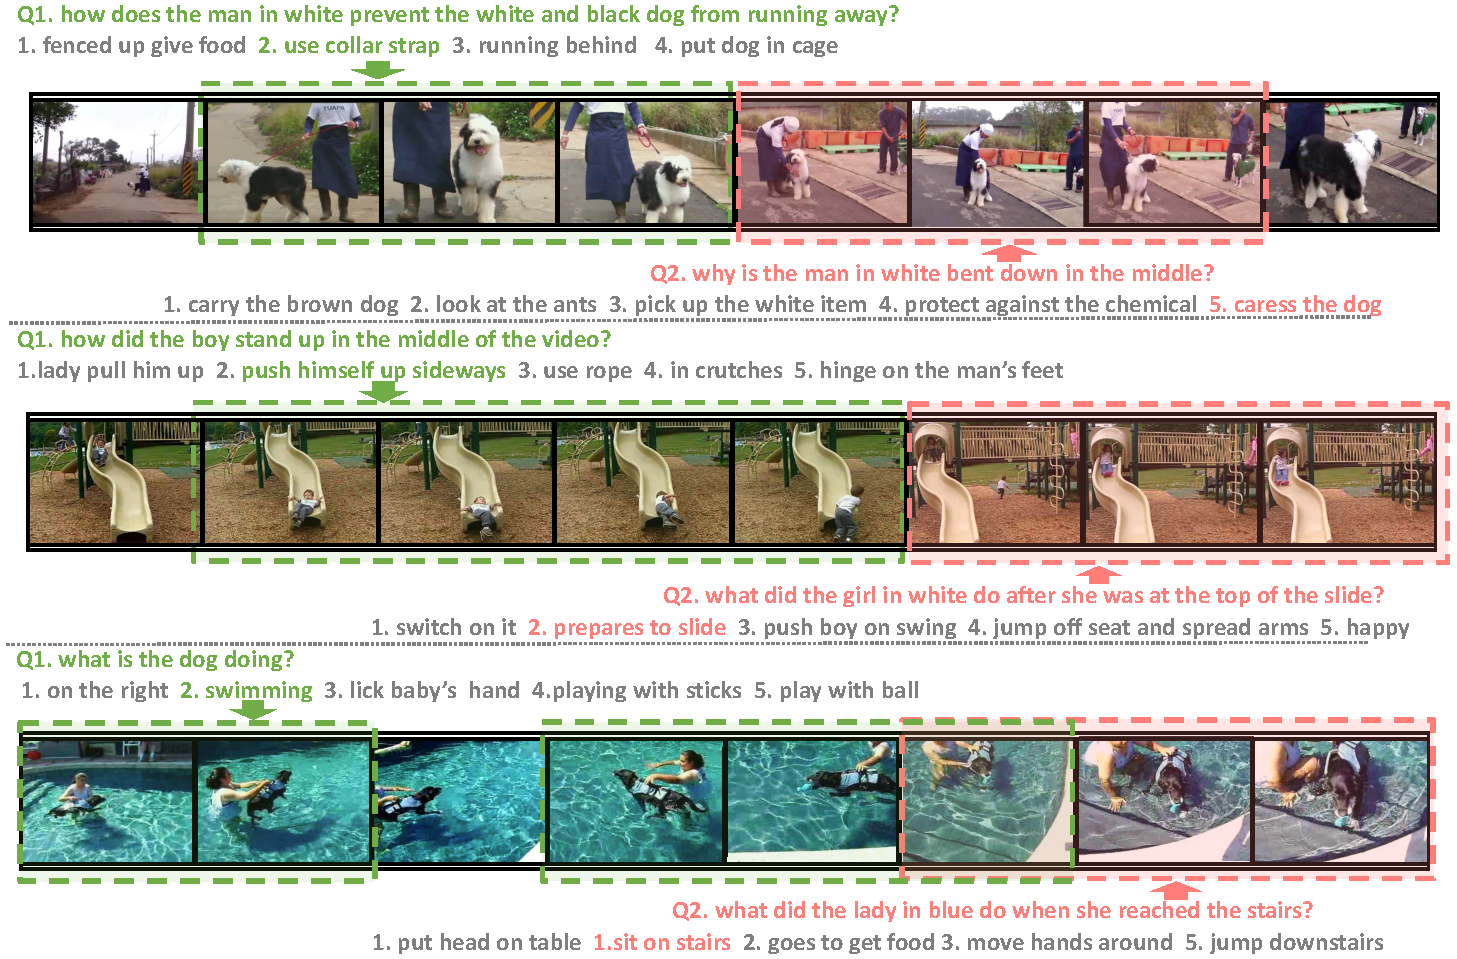
\includegraphics[width=0.97\textwidth]{fig/case.pdf}
 	\vspace{-13pt}
  \caption{Visualization of discovered grounding rationale. Each row comes with a video instance and two questions that target at different scene.  The \textcolor[rgb]{0,0.5,0}{green} and \textcolor[RGB]{225,152,150}{pink} windows indicate the rationales for the corresponding questions.}
  \label{fig:case-study}
 	\vspace{-10pt}
\end{figure*}

\vspace{5pt}
\noindent\textbf{Video Question Answering.}
Established to answer the question in dynamic visual content, VideoQA is bred through the task of ImageQA but has broadened its definition by assembling a temporal dimension. 
%
To make the task intriguing, the VideoQA benchmark has gone beyond the problem of description \cite{DBLP:conf/mm/XuZX0Z0Z17} and built several datasets to challenge temporal reasoning and even causal reflection \cite{DBLP:conf/cvpr/XiaoSYC21}. 
%
As a result, VideoQA has experienced an aggressive expansion in the architecture design. 
% 
Chronologically, early efforts tend to enact alignment through cross-modal attention \cite{zeng2016leveraging,li2019beyond} or enhanced memory design \cite{gao2018motionappearance, DBLP:conf/mm/XuZX0Z0Z17, fan2019heterogeneous}, while more recent works leverage the expressiveness of the graph neural network and perform the relation reasoning as node propagation \cite{jiang2020reasoning, DBLP:conf/mm/PengYBW21} or graph alignment \cite{park2021bridge}. 
%
In addition, current designs modify the representation of video and manipulate the temporal sequence from a hierarchical angle. Following this line, HCRN \cite{le2021hierarchical} first came out with the conditional relation module as building blocks that operate through different video intervals, whereas  HOSTR and PGAT made their advancement by incorporating visual content from different granularity. MSPAN, however, established cross-scale feature interaction on top of the hierarchy.
%
Despite effective, their intrinsic rationale has long been overlooked. To the best of our knowledge, EIGV is the first work that probes intrinsic interpretation. 

\vspace{5pt}
\noindent\textbf{Invariant Learning.}
% Given a encoder $f(\cdot)$ and input $x$, a representation $f(x)$ is equivariant to operation $G$, if $\forall x : f(G(x)) = T(G(x))$ ; Likewise, the property of invariance is defined as $\forall x : f(G(x)) = f(x)$. 
Given a encoder $f(\cdot)$ and input $x$, a representation $f(x)$ is invariant to operation $T$, if $\forall x : f(G(x)) = f(x)$. 
%
In practice, this invariant property has a long history in presenting visual content (\eg HOG \cite{DBLP:conf/mmm/HuangTHTJ11}), which has recently been renovated by deep learning in form of risk minimization. As its most prevailing form, IRM \cite{arjovsky2020invariant} fosters this philosophy by posing an environment invariant prior and discovering the underlying causal pattern by reducing cross-environment variance.   
% .that remains stable across different environments.
Different from previous studies that create environment via inductive re-grouping \cite{DBLP:conf/cvpr/AndersonWTB0S0G18} or adversarial inference \cite{DBLP:conf/icml/CreagerJZ21,wang2021causal, wang2022causal,wang2021clicks}, our method conducts causal intervention that perturbs the original sample distribution to form a new one.
\lyc{The most relvant work is \cite{Li_2022_CVPR}, where an invariant framework is introduced as a model-agnostic framework. However, EIGV gains better generalization ability by marrying equivariance as complementary learning principle.}
% Specifically, the discovery of  rationale implies two requirements on the partition:

\vspace{5pt}
\noindent\textbf{Visual Interpretability}
Machine interpretability can be achieved in various methods, such as clustering \cite{monnier2020dticlustering} or disentanglement \cite{shen2020interfacegan}. Our design can be vested in the category of attribution discovery, which investigates the contribution of different input elements toward the prediction. 
Based on whether the prediction and interpretation are yielded simultaneously, two categories are further defined: 1) post-hoc methods that generated the interpretation after prediction, such as backpropagation methods (\eg grad-CAM \cite{DBLP:conf/iccv/SelvarajuCDVPB17}). 2) self-interpretable method that cast prediction and interpretation at the same stage.
%
Unlike the post-hoc method that traces the interpretative clue from the output of the black-box, the self-interpretable model builds a transparency model via methods such as prototype generation \cite{DBLP:journals/corr/abs-1806-10574} or structural delineation \cite{wu2022dir}. 
%
In fact, previous works tend to focus on static image. EIGV, however, approaches the video interpretation in a multi-modal situation. 

\vspace{-5pt}
\section{conclusion}
\label{sec:conclusion}
In this paper, we present EIGV --- a model-agnostic explainer, that empowers the SoTA VideoQA model with intrinsic interpretability. In the light of the causality, we formulate our learning principles --- causal-equivariance and environment-invariance by incorporating three constituents, the grounding indicator, the intervener, and the disruptor, which manage a robust rationale discovery. Experiments across three benchmarks validate EIGV's fulfillment in both interpretation and accuracy.

% In addition to the technical advantages, we discuss possible refinements to improve the current design. Unlike some SoTAs that utilize object-level features (\eg HOSTR \cite{dang2021hierarchical} and PGAT \cite{DBLP:conf/mm/PengYBW21}), EIVG merely takes advantage of clip-level representation. Although the architecture of the backbone model is beyond the scope of this work, we anticipate that a fine-grained interpretation at the entity level will strengthen the current EIGV design.
% \section{Limitation and Complexity}
\label{section:limits}
\lyc{In addition to the technical advantages, we discuss possible limits of the current design. Unlike some SoTAs that utilize object-level features (\eg HOSTR \cite{dang2021hierarchical} and PGAT \cite{DBLP:conf/mm/PengYBW21}), EIVG merely takes advantage of clip-level representation. Although the architecture of the backbone model is beyond the scope of this work, we anticipate that a fine-grained interpretation at the entity level will strengthen the current EIGV design.
% 2) Current intervention strategy can possibly threaten the causal prediction by introducing context with new shortcuts. Since the scene intervener sample context stratification in a random manner, there is a slight chance to draw an undesired substitute that nested with strong static relation towards  a wrong answer, thus inducing a false prediction.
In terms of complexity, we run all experiments on NVIDIA Tesla V100 GPU, where our algorithm matched equally with the corresponding baseline.  For comparison, the backbone MSPAN model is trained for 1.5 hours till convergence on NExT-QA, whereas EIGV 
takes 1.6 hours.
}

%%
%% The next two lines define the bibliography style to be used, and
%% the bibliography file.

\bibliographystyle{ACM-Reference-Format}
\balance
\bibliography{sample-base}

%%
%% If your work has an appendix, this is the place to put it.
% \appendix


\end{sloppypar}
\end{document}
\endinput
%%
%% End of file `sample-sigconf.tex'.

\section{VideoQA Reformulation}
\label{sec:reformulation}

\wx{Here we argue that disclosing ``Which part of the video is critical to answering the question?'' is the key to presenting the visual-linguistic alignment explicitly.
To this end, we take a causal \cite{pearl2009causal} look at the reasoning process of VideoQA, then formalize it as a Structure Causal Model (SCM) \cite{pearl2016causal} by investigating the causal relationships among five variables: input video $V$, question $Q$, causal scene $C$, environment scene $E$, ground-truth answer $A$.
% Moreover, we analyze the conventional ERM scheme's limitations on
}

% Discovering the grounding rationale for faithful prediction requires careful inspection of the data generating process. In light of the causal theory \cite{pearl2016causal}, we revisit the formation of VideoQA models, then formalize them as a Structure Causal Model (SCM) \cite{pearl2009causal}  by investigating causality among five variables: input video $V$, question $Q$, causal scene $C$, environment scene $E$, ground-truth answer $A$.

\subsection{Causal Graph of VideoQA}\label{sec:causal-view}
\wx{Figure \ref{fig:scm} illustrates the causal graph, where each link depicts the cause-effect relationship between two variables:
\begin{itemize}[leftmargin=*]
    \item $Q\to C, E \gets V$. Given the question of interest $Q$, the video $V$ can be partitioned into two parts: (1) the causal scene $C$, which retains the question-critical information and naturally serves as the rationale for answering, (2) the environment scene $E$, which gathers the cues irrelevant to the question-answering. For example, to answering ``What is the girl doing?'' in Figure \ref{fig:overview}, $C$ should be the first two clips describing the ``girl-riding on-horse'' scene, while $E$ should be the last clip about the ``meadow'' scene. Moreover, the varying semantics of different questions will emphasize different $C$.
    \item $Q\rightarrow A \leftarrow C$. The visual knowledge in the causal scene $C$ and the linguistic semantics in the question $Q$ collaborate together to determine the answer $A$. Furthermore, this path, which presents the visual-linguistic alignment, internally interprets the reasoning.
    \item $E\dashleftarrow\dashrightarrow C$. The dashed arrow sketches additional probabilistic dependencies \cite{reason:Pearl09a} between $C$ and $E$, which typically arise from selection bias \cite{DBLP:conf/cvpr/TorralbaE11}. For example, the ``meadow'' scene is frequently collected as a common environment for the ``horse-riding'' scene. 
\end{itemize}}


\subsection{Beyond ERM}
\lyc{With inspections on prior VideoQA studies, we investigate their inability to distinguish the causal and non-causal effects of scenes.
Specifically, in conventional VideoQA models, video and question are directly paired together to model their interaction and approach the golden answer, consequently.
Inevitably, taking video as a whole leaves the contributions of scenes untouched, thus failing to differentiate $C$ from $E$ and forgoing their function divergence towards the answer.
Worse still, ERM enforces these models to blindly capture the statistical correlations between the video-question pairs and answers.
As such, the visual-linguistic alignment hinges easily on the spurious correlations between $E$ and $A$, owing to the backdoor paths \cite{pearl2016causal}, which hinders the generalization of models \cite{niu2020counterfactual,wu2022dir}.
Therefore, identifying the causal scene $C$ is the critical to addressing these limitations.}



\begin{figure}[t]
\centering
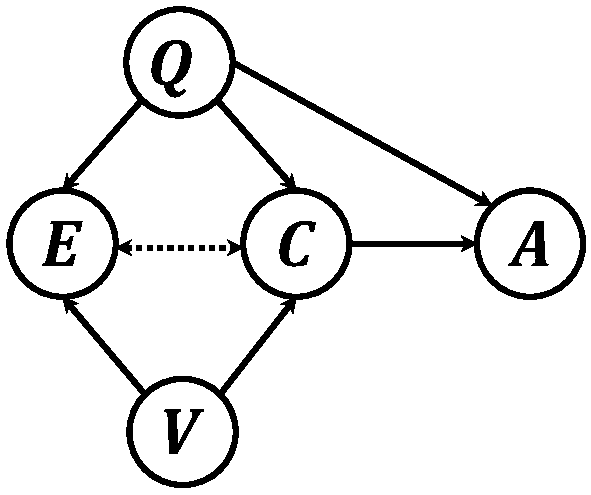
\includegraphics[scale=0.3]{fig/scm.pdf}
\vspace{-5pt}
\caption{Causal Graph of VideoQA}
\vspace{-10pt}
\label{fig:scm}
\end{figure}

\section{Experiment}
\label{sec:experiment}

In this section, we show the experimental results to answer the following research questions.
\begin{itemize}[leftmargin=*]
\item \textbf{RQ1} How effective is EIGV in discovering the causal pattern and improving the model generalization across different settings?
\item \textbf{RQ2} How does the sub-module and feature setting contribute to the performance?
\item \textbf{RQ3} What pattern does EIGV capture in rationale discovery?
\end{itemize}

\subsection{Settings}

\vspace{5pt}
\noindent \textbf{Datasets.} We conduct experiments on three benchmark datasets that challenge the model's reasoning capacity from different aspects: 
\textbf{MSVD-QA}  \cite{DBLP:conf/mm/XuZX0Z0Z17} and \textbf{MSRVTT-QA} \cite{DBLP:conf/mm/XuZX0Z0Z17} mainly emphasize the recognition ability by asking the descriptive questions, where 50K and 243K question-answer pairs are automatically generated from the human-labeled video captions, respectively.
\textbf{NExT-QA} \cite{DBLP:conf/cvpr/XiaoSYC21} pinpoints the causal and temporal relations among objects in the video. It contains 47.7K questions with answers in the form of multi-choice, which are manually annotated from 5.4K videos.

\vspace{5pt}
\noindent\textbf{Baseline.} We validate the effectiveness of EIGV across backbone VideoQA models of three kinds: 
1) \textbf{Memory-based} methods that foster a storage of input sequence via auxiliary memory design, such as AMU \cite{DBLP:conf/mm/XuZX0Z0Z17}, HME \cite{fan2019heterogeneous} and Co-Mem \cite{gao2018motionappearance}.
2) \textbf{Graph-based} methods that leverage the expressiveness of graph network to model the interaction between visual and language elements, which involves methods like L-GCN \cite{huang2020locationaware}, B2A  \cite{park2021bridge} and HGA \cite{jiang2020reasoning}. 
3) \textbf{Hierarchy-based} methods include HCRN \cite{le2021hierarchical}, PGAT \cite{DBLP:conf/mm/PengYBW21}, HOSTR \cite{dang2021hierarchical}, MSPAN \cite{DBLP:conf/acl/GuoZJ0L20} and HQGA \cite{xiao2021video}. In common, they exploit the multi-granularity nature of visual elements and realize the hierarchical reasoning via bottom-up architecture. 
In Specific, we test the generalization of EIGV by marrying our learning principles to three backbones of different categories: memory-based Co-Mem \cite{gao2018motionappearance}, graph-based HGA \cite{jiang2020reasoning} and hierarchy-based MSPAN \cite{DBLP:conf/acl/GuoZJ0L20}. 

\vspace{5pt}
\noindent \textbf{Implementation Detail.} 
For input representation, we encode the video instance as a sequence of $K$=16 clips, where each clip is represented as a combination of appearance and motion features extracted from the pre-trained ResNet-152 and 3D ResNeXt-101. For the linguistic feature, we follow \cite{DBLP:conf/cvpr/XiaoSYC21} and obtain the contextualized word representation using the fine-tuned BERT model. In the hyper-parameters setting, we set $d=512$ for cross-modal alignment, then train the model for 80 epochs with an initial learning rate of 5e-5.  During optimization, EIGV is trained with Adam optimizer and we decay the learning rate when validation stops improving for 5 epochs. The balance ratio $\beta$ is set to 0.75.
%for open-set QA and 0.025 for multi-choice QA. 

\subsection{Main Result (RQ1)}
\documentclass[lettersize,journal]{IEEEtran}
\usepackage{amsmath,amsfonts}
\usepackage{algorithmic}
\usepackage{algorithm}
\usepackage{array}
% \usepackage[caption=false,font=normalsize,labelfont=sf,textfont=sf]{subfig}
\usepackage{textcomp}
\usepackage{stfloats}
% \usepackage{xurl}
\usepackage{verbatim}
\usepackage{graphicx}
\usepackage{cite}
\usepackage{balance}
 
\usepackage{mathtools}
\usepackage{graphics, amsfonts, graphicx, amssymb, cite, mathrsfs}
% \let\proof\relax
% \let\endproof\relax
% \usepackage{amsthm}
% \usepackage{tikz}
% \usetikzlibrary{shapes,arrows}
% \usepackage{pgfplots}
\usepackage{color}
\usepackage[dvipsnames]{xcolor}
\usepackage{setspace}
% \usepackage[draft,bookmarks=false]{hyperref}
\usepackage{multirow}
\usepackage{rotating}
\usepackage{comment}
% \usepackage[keeplastbox]{flushend}
\usepackage[font=small]{caption}
% \usepackage{subcaption}
\usepackage[affil-it]{authblk}
% \usepackage{bm}
\usepackage{algorithm}
\usepackage{algorithmic}
\usepackage{enumitem}
% \usepackage{enumerate}
\usepackage{cite}
\usepackage{booktabs}
\usepackage{subcaption}
\usepackage{lipsum}

\PassOptionsToPackage{hyphens}{url}\usepackage{hyperref}

% \makeatletter
% \newcommand\fs@betterruled{%
%   \def\@fs@cfont{\bfseries}\let\@fs@capt\floatc@ruled
%   \def\@fs@pre{\vspace*{5pt}\hrule height.8pt depth0pt \kern2pt}%
%   \def\@fs@post{\kern2pt\hrule\relax}%
%   \def\@fs@mid{\kern2pt\hrule\kern2pt}%
%   \let\@fs@iftopcapt\iftrue}
% \floatstyle{betterruled}
% \restylefloat{algorithm}
% \makeatother


%
%%%%%%%%%%%%%%%%%%%%%%%%%%%%%%%%%theorem environments
%\newtheorem{assumption}{\hspace{0pt}\bf AS\hspace{-0.15cm}}
%\newtheorem{lemma}{\hspace{0pt}\bf Lemma}
%\newtheorem{proposition}{\hspace{0pt}\bf Proposition}
%\newtheorem{observation}{\hspace{0pt}\bf Observation}
%\newtheorem{theorem}{\hspace{0pt}\bf Theorem}
%\newtheorem{corollary}{\hspace{0pt}\bf Corollary}
%\newtheorem{fact}{\hspace{0pt}\bf Fact}
%\newtheorem{remark}{\hspace{0pt}\bf Remark}
%\newtheorem{test}{\hspace{0pt}\it Test Case}
%\newtheorem{definition}{\hspace{0pt}\bf Definition}
%\newtheorem{property}{\hspace{0pt}\bf Property}
%\newcommand {\mysubsubsection} [1] {\vspace{0.4cm}\noindent{\bf #1.}\addcontentsline{toc}{subsubsection}{\hspace{0pt}#1}}
%\newcommand {\mysubsection} [1]    {\vspace{0.4cm}\noindent{\bf #1.}\addcontentsline{toc}{subsection}{\hspace{0pt}#1}}



\newenvironment{myproof}[1][$\!\!$]{{\noindent\bf Proof #1: }}
                         {\hfill$\blacksquare$\medskip}

%%%%%%%%%%%%%%%%%%%%%%%%%%%%%%%%%list environment
\newenvironment{mylist}{\begin{list}{}{  \setlength{\itemsep  }{2pt} \setlength{\parsep    }{0in}
                                         \setlength{\parskip  }{0in} \setlength{\topsep    }{5pt}
                                         \setlength{\partopsep}{0in} \setlength{\leftmargin}{2pt}
                                         \setlength{\labelsep }{5pt} \setlength{\labelwidth}{-5pt}}}
                          {\end{list}\medskip}

\newcounter{excercise}
\newcounter{excercisepart}
\newcommand \excercise[1]{\addtocounter{excercise}{1} \setcounter{excercisepart}{0} \medskip
						  \noindent {\bf \theexcercise\ \, #1}}
\newcommand \excercisepart[1]{\addtocounter{excercisepart}{1} \medskip
						      \noindent {\it \Alph{excercisepart}\ \, #1}}


%%%%%%%%%%%%%%%%%%%%%%%%%%%%%%%%%list environment
%\newcounter{example}
%\newenvironment{example}[1]{\addtocounter{example}{1}\medskip \noindent{\it Example \theexample. #1.}}
%                           {\hfill\QED}%\newline\vspace{-2mm}\newline}


%%%%%%%%%%%%%%%%%%%%%%%%%%%%%%%%%slide equation environment
\newenvironment{slideeq} {              \begin{equation*}} {\end{equation*}            }
\newenvironment{nslideeq}{              \begin{equation*}} {\end{equation*}            }
\newenvironment{sslideeq}{\small        \begin{equation*}} {\end{equation*} \normalfont}
\newenvironment{fslideeq}{\footnotesize \begin{equation*}} {\end{equation*} \normalfont}
%%%%%%%%%%%%%%%%%%%%%%%%%%%%%%%%%slide equation environment
\newenvironment{slidealign} {              \begin{align*}} {\end{align*}            }
\newenvironment{nslidealign}{              \begin{align*}} {\end{align*}            }
\newenvironment{sslidealign}{\small        \begin{align*}} {\end{align*} \normalfont}
\newenvironment{fslidealign}{\footnotesize \begin{align*}} {\end{align*} \normalfont}

% Color definitions used in presentations
\definecolor{pennblue}{cmyk}{1,0.65,0,0.30}
\definecolor{pennred}{cmyk}{0,1,0.65,0.34}
\definecolor{mygreen}{rgb}{0.10,0.50,0.10}
\newcommand \red[1]         {{\color{red}#1}}
\newcommand \black[1]         {{\color{black}#1}}
\newcommand \blue[1]        {{\color{blue}#1}}
\newcommand \grey[1]        {{\color[rgb]{0.80,0.80,0.80}#1}}
\newcommand \gray[1]        {{\color[rgb]{0.80,0.80,0.80}#1}}
\newcommand \green[1]       {{\color[rgb]{0.10,0.50,0.10}#1}}
\newcommand \bulletcolor[1] {{\color{pennblue}#1}}
\def \arrowbullet {\bulletcolor{$\ \Rightarrow\ $}}
\def \arrbullet   {\bulletcolor{$\ \Rightarrow\ $}}
\def \ab          {\bulletcolor{$\ \Rightarrow\ $}}
\def \arritem     {\item[] \quad \arrowbullet}
\def \ai          {\item[] \quad \arrowbullet}
\def \doublearrow {\bulletcolor{$\ \Leftrightarrow\ $}}
\def \darrbullet  {\bulletcolor{$\ \Leftrightarrow\ $}}


%Always used
\def \defQfunction 
        {Q(u):=(1/\sqrt{2\pi})\int_u^\infty e^{-u^2/2} du}
\def \intinfty  { \int_{-\infty}^{\infty} }

%%%%%%%%%%%%%%%%%%%%%%%%%%%%%%%%% Overline
%
\def \ovP {\overline{P}}
\def \ovl {\overline{l}}
\def \ovbbl {\overline{\bbl}}
\def \ovX {\overline{X}}
\def \ovbbX {\overline{\bbX}}
\def \ovp {\overline{p}}
\def \ovbbp {\overline{\bbp}}
\def \ovr {\overline{r}}
\def \ova {\overline{a}}
\def \ovc {\overline{c}}
\def \ovalpha {\overline{\alpha}}

%%%%%%%%%%%%%%%%%%%%%%%%%%%%%%%%% Underline
%
\def \undP {\underline{P}}
\def \undl {\underline{l}}
\def \undbbl {\underline{\bbl}}
\def \undX {\underline{X}}
\def \undbbX {\underline{\bbX}}
\def \undp {\underline{p}}
\def \undbbp {\underline{\bbp}}
\def \undr {\underline{r}}
\def \unda {\underline{a}}
\def \undc {\underline{c}}
\def \undalpha {\underline{\alpha}}

%%%%%%%%%%%%%%%%%%%%%%%%%%%%%%%%% Overline and Underline
%
\def \undovP     {\underline{\ovP}}
\def \undovX     {\underline{\ovX}}
\def \undovbbX   {\underline{\ovbbX}}
\def \undovp     {\underline{\ovp}}
\def \undovbbp   {\underline{\ovbbp}}
\def \undovr     {\underline{\ovr}}
\def \undova     {\underline{\ova}}
\def \undovc     {\underline{\ovc}}
\def \undovalpha {\underline{\ovalpha}}

%roman symbols
\def \SNR     {\text{\normalfont SNR}   }
\def \ap      {\text{\normalfont ap}   }
\def \best    {\text{\normalfont best} }
\def \Co      {\text{\normalfont Co}   }
\def \Cov     {\text{\normalfont Cov}  }
\def \cov     {\text{\normalfont cov}  }
\def \dest    {\text{\normalfont dest} }
\def \diag    {\text{\normalfont diag} }
\def \eig     {\text{\normalfont eig}  }
\def \for     {\text{\normalfont for}  }
%\def \forall  {\text{\normalfont for all}  }
\def \forsome {\text{\normalfont for some}  }
\def \ML      {\text{\normalfont ML}   }
\def \MLE     {\text{\normalfont MLE}  }
\def \ml      {\text{\normalfont ml}   }
\def \mse     {\text{\normalfont mse}  }
\def \rank    {\text{\normalfont rank} }
\def \sign    {\text{\normalfont sign} }
\def \tr      {\text{\normalfont tr}   }

%units
\def \dB      {\, \text{\normalfont dB} }
\def \ms      {\, \text{\normalfont m}/ \text{\normalfont s}}
\def \kmh     {\, \text{\normalfont km}/ \text{\normalfont h}}
\def \m       {\, \text{\normalfont m} }
\def \s       {\, \text{\normalfont s} }
\def \sec     {\, \text{\normalfont sec.} }
\def \msec    {\, \text{\normalfont msec.} }
\def \cm      {\, \text{\normalfont cm} }
\def \km      {\, \text{\normalfont km} }
\def \GHz     {\, \text{\normalfont GHz} }
\def \Hz      {\, \text{\normalfont Hz} }
\def \MHZ     {\, \text{\normalfont MHz} }
\def \kHZ     {\, \text{\normalfont kHz} }


%Probability operators
\newcommand   \E     [1] {{\mathbb E}\left[#1\right]}
\newcommand   \Ec    [1] {{\mathbb E}\left(#1\right)}
\newcommand   \ind   [1] {{\mathbb I \left(#1\right)  } }
\renewcommand \Pr    [1] {\text{\normalfont Pr}  \left[#1\right]}
\newcommand   \Prc   [1] {\text{\normalfont Pr}  \left(#1\right)}
\renewcommand \P     [1] {\text{\normalfont P}   \left[#1\right]}
\newcommand   \Pc    [1] {\text{\normalfont P}   \left(#1\right)}
\newcommand   \Pcbig [1] {\text{\normalfont P}   \big(#1 \big)}
\newcommand   \PcBig [1] {\text{\normalfont P}   \Big(#1 \Big)}
\newcommand   \var   [1] {\text{\normalfont var} \left[#1\right]}
\newcommand   \varc  [1] {\text{\normalfont var} \left(#1\right)}
\renewcommand \Re    [1] {\text{\normalfont Re} \left(#1\right)}
\renewcommand \Im    [1] {\text{\normalfont Im} \left(#1\right)}
\newcommand   \der         [2] {\frac{\partial#1}{\partial#2}}
\newcommand   \inlineder   [2] {\partial#1/\partial#2}


%miscellaneous
\def \naturals {{\mathbb N}}
\def \reals    {{\mathbb R}}
\def \blog { {\bf \log   } }
\def \given{ {\,\big|\,  } }
\newcommand{\st}{\operatornamewithlimits{s.t.}}
\newcommand{\argmax}{\operatornamewithlimits{argmax}}
\newcommand{\argmin}{\operatornamewithlimits{argmin}}

%
%%%%%%%%%%%%%%%%%%%%%%%%%%%%%%%%%bar version
%capital alphabet
\def\bbarA{{\ensuremath{\bar A}}}
\def\bbarB{{\ensuremath{\bar B}}}
\def\bbarC{{\ensuremath{\bar C}}}
\def\bbarD{{\ensuremath{\bar D}}}
\def\bbarE{{\ensuremath{\bar E}}}
\def\bbarF{{\ensuremath{\bar F}}}
\def\bbarG{{\ensuremath{\bar G}}}
\def\bbarH{{\ensuremath{\bar H}}}
\def\bbarI{{\ensuremath{\bar I}}}
\def\bbarJ{{\ensuremath{\bar J}}}
\def\bbarK{{\ensuremath{\bar K}}}
\def\bbarL{{\ensuremath{\bar L}}}
\def\bbarM{{\ensuremath{\bar M}}}
\def\bbarN{{\ensuremath{\bar N}}}
\def\bbarO{{\ensuremath{\bar O}}}
\def\bbarP{{\ensuremath{\bar P}}}
\def\bbarQ{{\ensuremath{\bar Q}}}
\def\bbarR{{\ensuremath{\bar R}}}
\def\bbarW{{\ensuremath{\bar W}}}
\def\bbarU{{\ensuremath{\bar U}}}
\def\bbarV{{\ensuremath{\bar V}}}
\def\bbarS{{\ensuremath{\bar S}}}
\def\bbarT{{\ensuremath{\bar T}}}
\def\bbarX{{\ensuremath{\bar X}}}
\def\bbarY{{\ensuremath{\bar Y}}}
\def\bbarZ{{\ensuremath{\bar Z}}}
%lower case alphabet
\def\bbara{{\ensuremath{\bar a}}}
\def\bbarb{{\ensuremath{\bar b}}}
\def\bbarc{{\ensuremath{\bar c}}}
\def\bbard{{\ensuremath{\bar d}}}
\def\bbare{{\ensuremath{\bar e}}}
\def\bbarf{{\ensuremath{\bar f}}}
\def\bbarg{{\ensuremath{\bar g}}}
\def\bbarh{{\ensuremath{\bar h}}}
\def\bbari{{\ensuremath{\bar i}}}
\def\bbarj{{\ensuremath{\bar j}}}
\def\bbark{{\ensuremath{\bar k}}}
\def\bbarl{{\ensuremath{\bar l}}}
\def\bbarm{{\ensuremath{\bar m}}}
\def\bbarn{{\ensuremath{\bar n}}}
\def\bbaro{{\ensuremath{\bar o}}}
\def\bbarp{{\ensuremath{\bar p}}}
\def\bbarq{{\ensuremath{\bar q}}}
\def\bbarr{{\ensuremath{\bar r}}}
\def\bbarw{{\ensuremath{\bar w}}}
\def\bbaru{{\ensuremath{\bar u}}}
\def\bbarv{{\ensuremath{\bar v}}}
\def\bbars{{\ensuremath{\bar s}}}
\def\bbart{{\ensuremath{\bar t}}}
\def\bbarx{{\ensuremath{\bar x}}}
\def\bbary{{\ensuremath{\bar y}}}
\def\bbarz{{\ensuremath{\bar z}}}
%%%%%%%%%%%%%%%%%%%%%%%%%%%%%%%%%%end of bar version

%%%%%%%%%%%%%%%%%%%%%%%%%%%%%%%%%%%%%%%%%%%%%%%%%%%%%%%%%%%%%%%%%%%%%%%%%%%%%%%%%%%%%%%%%%%%%%%%
%%%   B   L   A   C   K   B   O   A   R   D         B   O   L   D   %%%%%%%%%%%%%%%%%%%%%%%%%%%%
%%%%%%%%%%%%%%%%%%%%%%%%%%%%%%%%%%%%%%%%%%%%%%%%%%%%%%%%%%%%%%%%%%%%%%%%%%%%%%%%%%%%%%%%%%%%%%%%
\def\mbA{{\ensuremath{\mathbb A}}}
\def\mbB{{\ensuremath{\mathbb B}}}
\def\mbC{{\ensuremath{\mathbb C}}}
\def\mbD{{\ensuremath{\mathbb D}}}
\def\mbE{{\ensuremath{\mathbb E}}}
\def\mbF{{\ensuremath{\mathbb F}}}
\def\mbG{{\ensuremath{\mathbb G}}}
\def\mbH{{\ensuremath{\mathbb H}}}
\def\mbI{{\ensuremath{\mathbb I}}}
\def\mbJ{{\ensuremath{\mathbb J}}}
\def\mbK{{\ensuremath{\mathbb K}}}
\def\mbL{{\ensuremath{\mathbb L}}}
\def\mbM{{\ensuremath{\mathbb M}}}
\def\mbN{{\ensuremath{\mathbb N}}}
\def\mbO{{\ensuremath{\mathbb O}}}
\def\mbP{{\ensuremath{\mathbb P}}}
\def\mbQ{{\ensuremath{\mathbb Q}}}
\def\mbR{{\ensuremath{\mathbb R}}}
\def\mbS{{\ensuremath{\mathbb S}}}
\def\mbT{{\ensuremath{\mathbb T}}}
\def\mbU{{\ensuremath{\mathbb U}}}
\def\mbV{{\ensuremath{\mathbb V}}}
\def\mbW{{\ensuremath{\mathbb W}}}
\def\mbX{{\ensuremath{\mathbb X}}}
\def\mbY{{\ensuremath{\mathbb Y}}}
\def\mbZ{{\ensuremath{\mathbb Z}}}
%%%%%%%%%%%%%%%%%%%%%%%%%%%%%%%%%%%%%%%%%%%%%%%%%%%%%%%%%%%%%%%%%%%%%%%%%%%%%%%%%%%%%%%%%%%%%%%%
%%%   C   A   L   I   G   R   A   P   H   I   C   %%%%%%%%%%%%%%%%%%%%%%%%%%%%%%%%%%%%%%%%%%%%%%
%%%%%%%%%%%%%%%%%%%%%%%%%%%%%%%%%%%%%%%%%%%%%%%%%%%%%%%%%%%%%%%%%%%%%%%%%%%%%%%%%%%%%%%%%%%%%%%%
\def\ccalA{{\ensuremath{\mathcal A}}}
\def\ccalB{{\ensuremath{\mathcal B}}}
\def\ccalC{{\ensuremath{\mathcal C}}}
\def\ccalD{{\ensuremath{\mathcal D}}}
\def\ccalE{{\ensuremath{\mathcal E}}}
\def\ccalF{{\ensuremath{\mathcal F}}}
\def\ccalG{{\ensuremath{\mathcal G}}}
\def\ccalH{{\ensuremath{\mathcal H}}}
\def\ccalI{{\ensuremath{\mathcal I}}}
\def\ccalJ{{\ensuremath{\mathcal J}}}
\def\ccalK{{\ensuremath{\mathcal K}}}
\def\ccalL{{\ensuremath{\mathcal L}}}
\def\ccalM{{\ensuremath{\mathcal M}}}
\def\ccalN{{\ensuremath{\mathcal N}}}
\def\ccalO{{\ensuremath{\mathcal O}}}
\def\ccalP{{\ensuremath{\mathcal P}}}
\def\ccalQ{{\ensuremath{\mathcal Q}}}
\def\ccalR{{\ensuremath{\mathcal R}}}
\def\ccalW{{\ensuremath{\mathcal W}}}
\def\ccalU{{\ensuremath{\mathcal U}}}
\def\ccalV{{\ensuremath{\mathcal V}}}
\def\ccalS{{\ensuremath{\mathcal S}}}
\def\ccalT{{\ensuremath{\mathcal T}}}
\def\ccalX{{\ensuremath{\mathcal X}}}
\def\ccalY{{\ensuremath{\mathcal Y}}}
\def\ccalZ{{\ensuremath{\mathcal Z}}}
%lower case alphabet
\def\ccala{{\ensuremath{\mathcal a}}}
\def\ccalb{{\ensuremath{\mathcal b}}}
\def\ccalc{{\ensuremath{\mathcal c}}}
\def\ccald{{\ensuremath{\mathcal d}}}
\def\ccale{{\ensuremath{\mathcal e}}}
\def\ccalf{{\ensuremath{\mathcal f}}}
\def\ccalg{{\ensuremath{\mathcal g}}}
\def\ccalh{{\ensuremath{\mathcal h}}}
\def\ccali{{\ensuremath{\mathcal i}}}
\def\ccalj{{\ensuremath{\mathcal j}}}
\def\ccalk{{\ensuremath{\mathcal k}}}
\def\ccall{{\ensuremath{\mathcal l}}}
\def\ccalm{{\ensuremath{\mathcal m}}}
\def\ccaln{{\ensuremath{\mathcal n}}}
\def\ccalo{{\ensuremath{\mathcal o}}}
\def\ccalp{{\ensuremath{\mathcal p}}}
\def\ccalq{{\ensuremath{\mathcal q}}}
\def\ccalr{{\ensuremath{\mathcal r}}}
\def\ccalw{{\ensuremath{\mathcal w}}}
\def\ccalu{{\ensuremath{\mathcal u}}}
\def\ccalv{{\ensuremath{\mathcal v}}}
\def\ccals{{\ensuremath{\mathcal s}}}
\def\ccalt{{\ensuremath{\mathcal t}}}
\def\ccalx{{\ensuremath{\mathcal x}}}
\def\ccaly{{\ensuremath{\mathcal y}}}
\def\ccalz{{\ensuremath{\mathcal z}}}
\def\ccal0{{\ensuremath{\mathcal 0}}}
%%%%%%%%%%%%%%%%%%%%%%%%%%%%%%%%%%%%%%%%%end of caligraph version
%
%
%%%%%%%%%%%%%%%%%%%%%%%%%%%%%%%%%%%%%%%%%%%hat version
%capital alphabet
\def\hhatA{{\ensuremath{\hat A}}}
\def\hhatB{{\ensuremath{\hat B}}}
\def\hhatC{{\ensuremath{\hat C}}}
\def\hhatD{{\ensuremath{\hat D}}}
\def\hhatE{{\ensuremath{\hat E}}}
\def\hhatF{{\ensuremath{\hat F}}}
\def\hhatG{{\ensuremath{\hat G}}}
\def\hhatH{{\ensuremath{\hat H}}}
\def\hhatI{{\ensuremath{\hat I}}}
\def\hhatJ{{\ensuremath{\hat J}}}
\def\hhatK{{\ensuremath{\hat K}}}
\def\hhatL{{\ensuremath{\hat L}}}
\def\hhatM{{\ensuremath{\hat M}}}
\def\hhatN{{\ensuremath{\hat N}}}
\def\hhatO{{\ensuremath{\hat O}}}
\def\hhatP{{\ensuremath{\hat P}}}
\def\hhatQ{{\ensuremath{\hat Q}}}
\def\hhatR{{\ensuremath{\hat R}}}
\def\hhatW{{\ensuremath{\hat W}}}
\def\hhatU{{\ensuremath{\hat U}}}
\def\hhatV{{\ensuremath{\hat V}}}
\def\hhatS{{\ensuremath{\hat S}}}
\def\hhatT{{\ensuremath{\hat T}}}
\def\hhatX{{\ensuremath{\hat X}}}
\def\hhatY{{\ensuremath{\hat Y}}}
\def\hhatZ{{\ensuremath{\hat Z}}}
%lower case alphabet
\def\hhata{{\ensuremath{\hat a}}}
\def\hhatb{{\ensuremath{\hat b}}}
\def\hhatc{{\ensuremath{\hat c}}}
\def\hhatd{{\ensuremath{\hat d}}}
\def\hhate{{\ensuremath{\hat e}}}
\def\hhatf{{\ensuremath{\hat f}}}
\def\hhatg{{\ensuremath{\hat g}}}
\def\hhath{{\ensuremath{\hat h}}}
\def\hhati{{\ensuremath{\hat i}}}
\def\hhatj{{\ensuremath{\hat j}}}
\def\hhatk{{\ensuremath{\hat k}}}
\def\hhatl{{\ensuremath{\hat l}}}
\def\hhatm{{\ensuremath{\hat m}}}
\def\hhatn{{\ensuremath{\hat n}}}
\def\hhato{{\ensuremath{\hat o}}}
\def\hhatp{{\ensuremath{\hat p}}}
\def\hhatq{{\ensuremath{\hat q}}}
\def\hhatr{{\ensuremath{\hat r}}}
\def\hhatw{{\ensuremath{\hat w}}}
\def\hhatu{{\ensuremath{\hat u}}}
\def\hhatv{{\ensuremath{\hat v}}}
\def\hhats{{\ensuremath{\hat s}}}
\def\hhatt{{\ensuremath{\hat t}}}
\def\hhatx{{\ensuremath{\hat x}}}
\def\hhaty{{\ensuremath{\hat y}}}
\def\hhatz{{\ensuremath{\hat z}}}
%%%%%%%%%%%%%%%%%%%%%%%%%%%%%%%%%%end of hat version
%
%
%%%%%%%%%%%%%%%%%%%%%%%%%%%%%%%%%%tilde version
%capital alphabet
\def\tdA{{\ensuremath{\tilde A}}}
\def\tdB{{\ensuremath{\tilde B}}}
\def\tdC{{\ensuremath{\tilde C}}}
\def\tdD{{\ensuremath{\tilde D}}}
\def\tdE{{\ensuremath{\tilde E}}}
\def\tdF{{\ensuremath{\tilde F}}}
\def\tdG{{\ensuremath{\tilde G}}}
\def\tdH{{\ensuremath{\tilde H}}}
\def\tdI{{\ensuremath{\tilde I}}}
\def\tdJ{{\ensuremath{\tilde J}}}
\def\tdK{{\ensuremath{\tilde K}}}
\def\tdL{{\ensuremath{\tilde L}}}
\def\tdM{{\ensuremath{\tilde M}}}
\def\tdN{{\ensuremath{\tilde N}}}
\def\tdO{{\ensuremath{\tilde O}}}
\def\tdP{{\ensuremath{\tilde P}}}
\def\tdQ{{\ensuremath{\tilde Q}}}
\def\tdR{{\ensuremath{\tilde R}}}
\def\tdW{{\ensuremath{\tilde W}}}
\def\tdU{{\ensuremath{\tilde U}}}
\def\tdV{{\ensuremath{\tilde V}}}
\def\tdS{{\ensuremath{\tilde S}}}
\def\tdT{{\ensuremath{\tilde T}}}
\def\tdX{{\ensuremath{\tilde X}}}
\def\tdY{{\ensuremath{\tilde Y}}}
\def\tdZ{{\ensuremath{\tilde Z}}}
%lower case alphabet
\def\tda{{\ensuremath{\tilde a}}}
\def\tdb{{\ensuremath{\tilde b}}}
\def\tdc{{\ensuremath{\tilde c}}}
\def\tdd{{\ensuremath{\tilde d}}}
\def\tde{{\ensuremath{\tilde e}}}
\def\tdf{{\ensuremath{\tilde f}}}
\def\tdg{{\ensuremath{\tilde g}}}
\def\tdh{{\ensuremath{\tilde h}}}
\def\tdi{{\ensuremath{\tilde i}}}
\def\tdj{{\ensuremath{\tilde j}}}
\def\tdk{{\ensuremath{\tilde k}}}
\def\tdl{{\ensuremath{\tilde l}}}
\def\tdm{{\ensuremath{\tilde m}}}
\def\tdn{{\ensuremath{\tilde n}}}
\def\tdo{{\ensuremath{\tilde o}}}
\def\tdp{{\ensuremath{\tilde p}}}
\def\tdq{{\ensuremath{\tilde q}}}
\def\tdr{{\ensuremath{\tilde r}}}
\def\tdw{{\ensuremath{\tilde w}}}
\def\tdu{{\ensuremath{\tilde u}}}
\def\tdv{{\ensuremath{\tilde r}}}
\def\tds{{\ensuremath{\tilde s}}}
\def\tdt{{\ensuremath{\tilde t}}}
\def\tdx{{\ensuremath{\tilde x}}}
\def\tdy{{\ensuremath{\tilde y}}}
\def\tdz{{\ensuremath{\tilde z}}}
%%%%%%%%%%%%%%%%%%%%%%%%%%%%%%%%%%%%end of tilde version
%
%%%%%%%%%%%%%%%%%%%%%%%%%%%%%%%%%%%%%check version
%lower case alphabet
\def\chka{{\ensuremath{\check a}}}
\def\chkb{{\ensuremath{\check b}}}
\def\chkc{{\ensuremath{\check c}}}
\def\chkd{{\ensuremath{\check d}}}
\def\chke{{\ensuremath{\check e}}}
\def\chkf{{\ensuremath{\check f}}}
\def\chkg{{\ensuremath{\check g}}}
\def\chkh{{\ensuremath{\check h}}}
\def\chki{{\ensuremath{\check i}}}
\def\chkj{{\ensuremath{\check j}}}
\def\chkk{{\ensuremath{\check k}}}
\def\chkl{{\ensuremath{\check l}}}
\def\chkm{{\ensuremath{\check m}}}
\def\chkn{{\ensuremath{\check n}}}
\def\chko{{\ensuremath{\check o}}}
\def\chkp{{\ensuremath{\check p}}}
\def\chkq{{\ensuremath{\check q}}}
\def\chkr{{\ensuremath{\check r}}}
\def\chkw{{\ensuremath{\check w}}}
\def\chku{{\ensuremath{\check u}}}
\def\chkv{{\ensuremath{\check v}}}
\def\chks{{\ensuremath{\check s}}}
\def\chkt{{\ensuremath{\check t}}}
\def\chkx{{\ensuremath{\check x}}}
\def\chky{{\ensuremath{\check y}}}
\def\chkz{{\ensuremath{\check z}}}
%%%%%%%%%%%%%%%%%%%%%%%%%%%%%%%%%%end of check version
%
%
%%%%%%%%%%%%%%%%%%%%%%%%%%%%%%%%%%%%Bold version
% upper case bold
\def\bbone{{\ensuremath{\mathbf 1}}}
\def\bbzero{{\ensuremath{\mathbf 0}}}
\def\bbA{{\ensuremath{\mathbf A}}}
\def\bbB{{\ensuremath{\mathbf B}}}
\def\bbC{{\ensuremath{\mathbf C}}}
\def\bbD{{\ensuremath{\mathbf D}}}
\def\bbE{{\ensuremath{\mathbf E}}}
\def\bbF{{\ensuremath{\mathbf F}}}
\def\bbG{{\ensuremath{\mathbf G}}}
\def\bbH{{\ensuremath{\mathbf H}}}
\def\bbI{{\ensuremath{\mathbf I}}}
\def\bbJ{{\ensuremath{\mathbf J}}}
\def\bbK{{\ensuremath{\mathbf K}}}
\def\bbL{{\ensuremath{\mathbf L}}}
\def\bbM{{\ensuremath{\mathbf M}}}
\def\bbN{{\ensuremath{\mathbf N}}}
\def\bbO{{\ensuremath{\mathbf O}}}
\def\bbP{{\ensuremath{\mathbf P}}}
\def\bbQ{{\ensuremath{\mathbf Q}}}
\def\bbR{{\ensuremath{\mathbf R}}}
\def\bbW{{\ensuremath{\mathbf W}}}
\def\bbU{{\ensuremath{\mathbf U}}}
\def\bbV{{\ensuremath{\mathbf V}}}
\def\bbS{{\ensuremath{\mathbf S}}}
\def\bbT{{\ensuremath{\mathbf T}}}
\def\bbX{{\ensuremath{\mathbf X}}}
\def\bbY{{\ensuremath{\mathbf Y}}}
\def\bbZ{{\ensuremath{\mathbf Z}}}
%lower case bold
\def\bba{{\ensuremath{\mathbf a}}}
\def\bbb{{\ensuremath{\mathbf b}}}
\def\bbc{{\ensuremath{\mathbf c}}}
\def\bbd{{\ensuremath{\mathbf d}}}
\def\bbe{{\ensuremath{\mathbf e}}}
\def\bbf{{\ensuremath{\mathbf f}}}
\def\bbg{{\ensuremath{\mathbf g}}}
\def\bbh{{\ensuremath{\mathbf h}}}
\def\bbi{{\ensuremath{\mathbf i}}}
\def\bbj{{\ensuremath{\mathbf j}}}
\def\bbk{{\ensuremath{\mathbf k}}}
\def\bbl{{\ensuremath{\mathbf l}}}
\def\bbm{{\ensuremath{\mathbf m}}}
\def\bbn{{\ensuremath{\mathbf n}}}
\def\bbo{{\ensuremath{\mathbf o}}}
\def\bbp{{\ensuremath{\mathbf p}}}
\def\bbq{{\ensuremath{\mathbf q}}}
\def\bbr{{\ensuremath{\mathbf r}}}
\def\bbw{{\ensuremath{\mathbf w}}}
\def\bbu{{\ensuremath{\mathbf u}}}
\def\bbv{{\ensuremath{\mathbf v}}}
\def\bbs{{\ensuremath{\mathbf s}}}
\def\bbt{{\ensuremath{\mathbf t}}}
\def\bbx{{\ensuremath{\mathbf x}}}
\def\bby{{\ensuremath{\mathbf y}}}
\def\bbz{{\ensuremath{\mathbf z}}}
\def\bb0{{\ensuremath{\mathbf 0}}}
%

% roman 
\def\rmA{{\ensuremath\text{A}}}
\def\rmB{{\ensuremath\text{B}}}
\def\rmC{{\ensuremath\text{C}}}
\def\rmD{{\ensuremath\text{D}}}
\def\rmE{{\ensuremath\text{E}}}
\def\rmF{{\ensuremath\text{F}}}
\def\rmG{{\ensuremath\text{G}}}
\def\rmH{{\ensuremath\text{H}}}
\def\rmI{{\ensuremath\text{I}}}
\def\rmJ{{\ensuremath\text{J}}}
\def\rmK{{\ensuremath\text{K}}}
\def\rmL{{\ensuremath\text{L}}}
\def\rmM{{\ensuremath\text{M}}}
\def\rmN{{\ensuremath\text{N}}}
\def\rmO{{\ensuremath\text{O}}}
\def\rmP{{\ensuremath\text{P}}}
\def\rmQ{{\ensuremath\text{Q}}}
\def\rmR{{\ensuremath\text{R}}}
\def\rmW{{\ensuremath\text{W}}}
\def\rmU{{\ensuremath\text{U}}}
\def\rmV{{\ensuremath\text{V}}}
\def\rmS{{\ensuremath\text{S}}}
\def\rmT{{\ensuremath\text{T}}}
\def\rmX{{\ensuremath\text{X}}}
\def\rmY{{\ensuremath\text{Y}}}
\def\rmZ{{\ensuremath\text{Z}}}
%lower case bold
\def\rma{{\ensuremath\text{a}}}
\def\rmb{{\ensuremath\text{b}}}
\def\rmc{{\ensuremath\text{c}}}
\def\rmd{{\ensuremath\text{d}}}
\def\rme{{\ensuremath\text{e}}}
\def\rmf{{\ensuremath\text{f}}}
\def\rmg{{\ensuremath\text{g}}}
\def\rmh{{\ensuremath\text{h}}}
\def\rmi{{\ensuremath\text{i}}}
\def\rmj{{\ensuremath\text{j}}}
\def\rmk{{\ensuremath\text{k}}}
\def\rml{{\ensuremath\text{l}}}
\def\rmm{{\ensuremath\text{m}}}
\def\rmn{{\ensuremath\text{n}}}
\def\rmo{{\ensuremath\text{o}}}
\def\rmp{{\ensuremath\text{p}}}
\def\rmq{{\ensuremath\text{q}}}
\def\rmr{{\ensuremath\text{r}}}
\def\rmw{{\ensuremath\text{w}}}
\def\rmu{{\ensuremath\text{u}}}
\def\rmv{{\ensuremath\text{v}}}
\def\rms{{\ensuremath\text{s}}}
\def\rmt{{\ensuremath\text{t}}}
\def\rmx{{\ensuremath\text{x}}}
\def\rmy{{\ensuremath\text{y}}}
\def\rmz{{\ensuremath\text{z}}}
%


%%%%%%%%%%%%%%%%%%%%%%%%%%%%%%%%%%%%%%%%%%%%%%bar bold version
%upper case
%
\def\barbA{{\bar{\ensuremath{\mathbf A}} }}
\def\barbB{{\bar{\ensuremath{\mathbf B}} }}
\def\barbC{{\bar{\ensuremath{\mathbf C}} }}
\def\barbD{{\bar{\ensuremath{\mathbf D}} }}
\def\barbE{{\bar{\ensuremath{\mathbf E}} }}
\def\barbF{{\bar{\ensuremath{\mathbf F}} }}
\def\barbG{{\bar{\ensuremath{\mathbf G}} }}
\def\barbH{{\bar{\ensuremath{\mathbf H}} }}
\def\barbI{{\bar{\ensuremath{\mathbf I}} }}
\def\barbJ{{\bar{\ensuremath{\mathbf J}} }}
\def\barbK{{\bar{\ensuremath{\mathbf K}} }}
\def\barbL{{\bar{\ensuremath{\mathbf L}} }}
\def\barbM{{\bar{\ensuremath{\mathbf M}} }}
\def\barbN{{\bar{\ensuremath{\mathbf N}} }}
\def\barbO{{\bar{\ensuremath{\mathbf O}} }}
\def\barbP{{\bar{\ensuremath{\mathbf P}} }}
\def\barbQ{{\bar{\ensuremath{\mathbf Q}} }}
\def\barbR{{\bar{\ensuremath{\mathbf R}} }}
\def\barbS{{\bar{\ensuremath{\mathbf S}} }}
\def\barbT{{\bar{\ensuremath{\mathbf T}} }}
\def\barbU{{\bar{\ensuremath{\mathbf U}} }}
\def\barbV{{\bar{\ensuremath{\mathbf V}} }}
\def\barbW{{\bar{\ensuremath{\mathbf W}} }}
\def\barbX{{\overline{\bbX}}}
\def\barbY{{\bar{\ensuremath{\mathbf Y}} }}
\def\barbZ{{\bar{\ensuremath{\mathbf Z}} }}
%
%lower case
%
\def\barba{{\bar{\ensuremath{\mathbf a}} }}
\def\barbb{{\bar{\ensuremath{\mathbf b}} }}
\def\barbc{{\bar{\ensuremath{\mathbf c}} }}
\def\barbd{{\bar{\ensuremath{\mathbf d}} }}
\def\barbe{{\bar{\ensuremath{\mathbf e}} }}
\def\barbf{{\bar{\ensuremath{\mathbf f}} }}
\def\barbg{{\bar{\ensuremath{\mathbf g}} }}
\def\barbh{{\bar{\ensuremath{\mathbf h}} }}
\def\barbi{{\bar{\ensuremath{\mathbf i}} }}
\def\barbj{{\bar{\ensuremath{\mathbf j}} }}
\def\barbk{{\bar{\ensuremath{\mathbf k}} }}
\def\barbl{{\bar{\ensuremath{\mathbf l}} }}
\def\barbm{{\bar{\ensuremath{\mathbf m}} }}
\def\barbn{{\bar{\ensuremath{\mathbf n}} }}
\def\barbo{{\bar{\ensuremath{\mathbf o}} }}
\def\barbp{{\bar{\ensuremath{\mathbf p}} }}
\def\barbq{{\bar{\ensuremath{\mathbf q}} }}
\def\barbr{{\bar{\ensuremath{\mathbf r}} }}
\def\barbs{{\bar{\ensuremath{\mathbf s}} }}
\def\barbt{{\bar{\ensuremath{\mathbf t}} }}
\def\barbu{{\bar{\ensuremath{\mathbf u}} }}
\def\barbv{{\bar{\ensuremath{\mathbf v}} }}
\def\barbw{{\bar{\ensuremath{\mathbf w}} }}
\def\barbx{{\bar{\ensuremath{\mathbf x}} }}
\def\barby{{\bar{\ensuremath{\mathbf y}} }}
\def\barbz{{\bar{\ensuremath{\mathbf z}} }}
%%%%%%%%%%%%%%%%%%%%%%%%%%%%%%%%%%%%%%%%%%%%%%%end of bar bold bersion
%
%
%%%%%%%%%%%%%%%%%%%%%%%%%%%%%%%%%%%%%%%%%%%%%%hat bold version
%upper case
%
\def\hbA{{\hat{\ensuremath{\mathbf A}} }}
\def\hbB{{\hat{\ensuremath{\mathbf B}} }}
\def\hbC{{\hat{\ensuremath{\mathbf C}} }}
\def\hbD{{\hat{\ensuremath{\mathbf D}} }}
\def\hbE{{\hat{\ensuremath{\mathbf E}} }}
\def\hbF{{\hat{\ensuremath{\mathbf F}} }}
\def\hbG{{\hat{\ensuremath{\mathbf G}} }}
\def\hbH{{\hat{\ensuremath{\mathbf H}} }}
\def\hbI{{\hat{\ensuremath{\mathbf I}} }}
\def\hbJ{{\hat{\ensuremath{\mathbf J}} }}
\def\hbK{{\hat{\ensuremath{\mathbf K}} }}
\def\hbL{{\hat{\ensuremath{\mathbf L}} }}
\def\hbM{{\hat{\ensuremath{\mathbf M}} }}
\def\hbN{{\hat{\ensuremath{\mathbf N}} }}
\def\hbO{{\hat{\ensuremath{\mathbf O}} }}
\def\hbP{{\hat{\ensuremath{\mathbf P}} }}
\def\hbQ{{\hat{\ensuremath{\mathbf Q}} }}
\def\hbR{{\hat{\ensuremath{\mathbf R}} }}
\def\hbS{{\hat{\ensuremath{\mathbf S}} }}
\def\hbT{{\hat{\ensuremath{\mathbf T}} }}
\def\hbU{{\hat{\ensuremath{\mathbf U}} }}
\def\hbV{{\hat{\ensuremath{\mathbf V}} }}
\def\hbW{{\hat{\ensuremath{\mathbf W}} }}
\def\hbX{{\hat{\ensuremath{\mathbf X}} }}
\def\hbY{{\hat{\ensuremath{\mathbf Y}} }}
\def\hbZ{{\hat{\ensuremath{\mathbf Z}} }}
%
%lower case
%
\def\hba{{\hat{\ensuremath{\mathbf a}} }}
\def\hbb{{\hat{\ensuremath{\mathbf b}} }}
\def\hbc{{\hat{\ensuremath{\mathbf c}} }}
\def\hbd{{\hat{\ensuremath{\mathbf d}} }}
\def\hbe{{\hat{\ensuremath{\mathbf e}} }}
\def\hbf{{\hat{\ensuremath{\mathbf f}} }}
\def\hbg{{\hat{\ensuremath{\mathbf g}} }}
\def\hbh{{\hat{\ensuremath{\mathbf h}} }}
\def\hbi{{\hat{\ensuremath{\mathbf i}} }}
\def\hbj{{\hat{\ensuremath{\mathbf j}} }}
\def\hbk{{\hat{\ensuremath{\mathbf k}} }}
\def\hbl{{\hat{\ensuremath{\mathbf l}} }}
\def\hbm{{\hat{\ensuremath{\mathbf m}} }}
\def\hbn{{\hat{\ensuremath{\mathbf n}} }}
\def\hbo{{\hat{\ensuremath{\mathbf o}} }}
\def\hbp{{\hat{\ensuremath{\mathbf p}} }}
\def\hbq{{\hat{\ensuremath{\mathbf q}} }}
\def\hbr{{\hat{\ensuremath{\mathbf r}} }}
\def\hbs{{\hat{\ensuremath{\mathbf s}} }}
\def\hbt{{\hat{\ensuremath{\mathbf t}} }}
\def\hbu{{\hat{\ensuremath{\mathbf u}} }}
\def\hbv{{\hat{\ensuremath{\mathbf v}} }}
\def\hbw{{\hat{\ensuremath{\mathbf w}} }}
\def\hbx{{\hat{\ensuremath{\mathbf x}} }}
\def\hby{{\hat{\ensuremath{\mathbf y}} }}
\def\hbz{{\hat{\ensuremath{\mathbf z}} }}
%%%%%%%%%%%%%%%%%%%%%%%%%%%%%%%%%%%%%%%%%%%%%%%end of hat bold  bersion
%
%
%%%%%%%%%%%%%%%%%%%%%%%%%%%%%%%%%%%%%%%%%%%%%%tilde bold version
%upper case
%
\def\tbA{{\tilde{\ensuremath{\mathbf A}} }}
\def\tbB{{\tilde{\ensuremath{\mathbf B}} }}
\def\tbC{{\tilde{\ensuremath{\mathbf C}} }}
\def\tbD{{\tilde{\ensuremath{\mathbf D}} }}
\def\tbE{{\tilde{\ensuremath{\mathbf E}} }}
\def\tbF{{\tilde{\ensuremath{\mathbf F}} }}
\def\tbG{{\tilde{\ensuremath{\mathbf G}} }}
\def\tbH{{\tilde{\ensuremath{\mathbf H}} }}
\def\tbI{{\tilde{\ensuremath{\mathbf I}} }}
\def\tbJ{{\tilde{\ensuremath{\mathbf J}} }}
\def\tbK{{\tilde{\ensuremath{\mathbf K}} }}
\def\tbL{{\tilde{\ensuremath{\mathbf L}} }}
\def\tbM{{\tilde{\ensuremath{\mathbf M}} }}
\def\tbN{{\tilde{\ensuremath{\mathbf N}} }}
\def\tbO{{\tilde{\ensuremath{\mathbf O}} }}
\def\tbP{{\tilde{\ensuremath{\mathbf P}} }}
\def\tbQ{{\tilde{\ensuremath{\mathbf Q}} }}
\def\tbR{{\tilde{\ensuremath{\mathbf R}} }}
\def\tbS{{\tilde{\ensuremath{\mathbf S}} }}
\def\tbT{{\tilde{\ensuremath{\mathbf T}} }}
\def\tbU{{\tilde{\ensuremath{\mathbf U}} }}
\def\tbV{{\tilde{\ensuremath{\mathbf V}} }}
\def\tbW{{\tilde{\ensuremath{\mathbf W}} }}
\def\tbX{{\tilde{\ensuremath{\mathbf X}} }}
\def\tbY{{\tilde{\ensuremath{\mathbf Y}} }}
\def\tbZ{{\tilde{\ensuremath{\mathbf Z}} }}
%
%lower case
%
\def\tba{{\tilde{\ensuremath{\mathbf a}} }}
\def\tbb{{\tilde{\ensuremath{\mathbf b}} }}
\def\tbc{{\tilde{\ensuremath{\mathbf c}} }}
\def\tbd{{\tilde{\ensuremath{\mathbf d}} }}
\def\tbe{{\tilde{\ensuremath{\mathbf e}} }}
\def\tbf{{\tilde{\ensuremath{\mathbf f}} }}
\def\tbg{{\tilde{\ensuremath{\mathbf g}} }}
\def\tbh{{\tilde{\ensuremath{\mathbf h}} }}
\def\tbi{{\tilde{\ensuremath{\mathbf i}} }}
\def\tbj{{\tilde{\ensuremath{\mathbf j}} }}
\def\tbk{{\tilde{\ensuremath{\mathbf k}} }}
\def\tbl{{\tilde{\ensuremath{\mathbf l}} }}
\def\tbm{{\tilde{\ensuremath{\mathbf m}} }}
\def\tbn{{\tilde{\ensuremath{\mathbf n}} }}
\def\tbo{{\tilde{\ensuremath{\mathbf o}} }}
\def\tbp{{\tilde{\ensuremath{\mathbf p}} }}
\def\tbq{{\tilde{\ensuremath{\mathbf q}} }}
\def\tbr{{\tilde{\ensuremath{\mathbf r}} }}
\def\tbs{{\tilde{\ensuremath{\mathbf s}} }}
\def\tbt{{\tilde{\ensuremath{\mathbf t}} }}
\def\tbu{{\tilde{\ensuremath{\mathbf u}} }}
\def\tbv{{\tilde{\ensuremath{\mathbf v}} }}
\def\tbw{{\tilde{\ensuremath{\mathbf w}} }}
\def\tbx{{\tilde{\ensuremath{\mathbf x}} }}
\def\tby{{\tilde{\ensuremath{\mathbf y}} }}
\def\tbz{{\tilde{\ensuremath{\mathbf z}} }}
%%%%%%%%%%%%%%%%%%%%%%%%%%%%%%%%%%%%%%%%%%%%%%%end of tilde bold  bersion
%
%%%%%%%%%%%%%%%%%%%%%%%%%%%%%%%%%%%%%%%%%%%%%%%bold caligraph
%
\def\bbcalA{\mbox{\boldmath $\mathcal{A}$}}
\def\bbcalB{\mbox{\boldmath $\mathcal{B}$}}
\def\bbcalC{\mbox{\boldmath $\mathcal{C}$}}
\def\bbcalD{\mbox{\boldmath $\mathcal{D}$}}
\def\bbcalE{\mbox{\boldmath $\mathcal{E}$}}
\def\bbcalF{\mbox{\boldmath $\mathcal{F}$}}
\def\bbcalG{\mbox{\boldmath $\mathcal{G}$}}
\def\bbcalH{\mbox{\boldmath $\mathcal{H}$}}
\def\bbcalI{\mbox{\boldmath $\mathcal{I}$}}
\def\bbcalJ{\mbox{\boldmath $\mathcal{J}$}}
\def\bbcalK{\mbox{\boldmath $\mathcal{K}$}}
\def\bbcalL{\mbox{\boldmath $\mathcal{L}$}}
\def\bbcalM{\mbox{\boldmath $\mathcal{M}$}}
\def\bbcalN{\mbox{\boldmath $\mathcal{N}$}}
\def\bbcalO{\mbox{\boldmath $\mathcal{O}$}}
\def\bbcalP{\mbox{\boldmath $\mathcal{P}$}}
\def\bbcalQ{\mbox{\boldmath $\mathcal{Q}$}}
\def\bbcalR{\mbox{\boldmath $\mathcal{R}$}}
\def\bbcalW{\mbox{\boldmath $\mathcal{W}$}}
\def\bbcalU{\mbox{\boldmath $\mathcal{U}$}}
\def\bbcalV{\mbox{\boldmath $\mathcal{V}$}}
\def\bbcalS{\mbox{\boldmath $\mathcal{S}$}}
\def\bbcalT{\mbox{\boldmath $\mathcal{T}$}}
\def\bbcalX{\mbox{\boldmath $\mathcal{X}$}}
\def\bbcalY{\mbox{\boldmath $\mathcal{Y}$}}
\def\bbcalZ{\mbox{\boldmath $\mathcal{Z}$}}
%
%%%%%%%%%%%%%%%%%%%%%%%%%%%%%%%%%%%%%%%%%%%%%%%%%%end of caligraph
%
%
%
%
%%%%%%%%%%%%%%%%%%%%%%%%%%%%%%%%%%%%%%%%%%%%%%%tilde Greek
%
\def\tdupsilon{\tilde\upsilon}
\def\tdalpha{\tilde\alpha}
\def\tbeta{\tilde\beta}
\def\tdgamma{\tilde\gamma}
\def\tddelta{\tilde\delta}
\def\tdepsilon{\tilde\epsilon}
\def\tdvarepsilon{\tilde\varepsilon}
\def\tdzeta{\tilde\zeta}
\def\tdeta{\tilde\eta}
\def\tdtheta{\tilde\theta}
\def\tdvartheta{\tilde\vartheta}

\def\tdiota{\tilde\iota}
\def\tdkappa{\tilde\kappa}
\def\tdlambda{\tilde\lambda}
\def\tdmu{\tilde\mu}
\def\tdnu{\tilde\nu}
\def\tdxi{\tilde\xi}
\def\tdpi{\tilde\pi}
\def\tdrho{\tilde\rho}
\def\tdvarrho{\tilde\varrho}
\def\tdsigma{\tilde\sigma}
\def\tdvarsigma{\tilde\varsigma}
\def\tdtau{\tilde\tau}
\def\tdupsilon{\tilde\upsilon}
\def\tdphi{\tilde\phi}
\def\tdvarphi{\tilde\varphi}
\def\tdchi{\tilde\chi}
\def\tdpsi{\tilde\psi}
\def\tdomega{\tilde\omega}

\def\tdGamma{\tilde\Gamma}
\def\tdDelta{\tilde\Delta}
\def\tdTheta{\tilde\Theta}
\def\tdLambda{\tilde\Lambda}
\def\tdXi{\tilde\Xi}
\def\tdPi{\tilde\Pi}
\def\tdSigma{\tilde\Sigma}
\def\tdUpsilon{\tilde\Upsilon}
\def\tdPhi{\tilde\Phi}
\def\tdPsi{\tilde\Psi}
%%%%%%%%%%%%%%%%%%%%%%%%%%%%%%%%%%%%%%%%%%%end of title  Greek
%
%%%%%%%%%%%%%%%%%%%%%%%%%%%%%%%%%%%%%%%%%%%%%%%bar Greek
%
\def\bbarupsilon{\bar\upsilon}
\def\bbaralpha{\bar\alpha}
\def\bbarbeta{\bar\beta}
\def\bbargamma{\bar\gamma}
\def\bbardelta{\bar\delta}
\def\bbarepsilon{\bar\epsilon}
\def\bbarvarepsilon{\bar\varepsilon}
\def\bbarzeta{\bar\zeta}
\def\bbareta{\bar\eta}
\def\bbartheta{\bar\theta}
\def\bbarvartheta{\bar\vartheta}

\def\bbariota{\bar\iota}
\def\bbarkappa{\bar\kappa}
\def\bbarlambda{\bar\lambda}
\def\bbarmu{\bar\mu}
\def\bbarnu{\bar\nu}
\def\bbarxi{\bar\xi}
\def\bbarpi{\bar\pi}
\def\bbarrho{\bar\rho}
\def\bbarvarrho{\bar\varrho}
\def\bbarvarsigma{\bar\varsigma}
\def\bbarphi{\bar\phi}
\def\bbarvarphi{\bar\varphi}
\def\bbarchi{\bar\chi}
\def\bbarpsi{\bar\psi}
\def\bbaromega{\bar\omega}

\def\bbarGamma{\bar\Gamma}
\def\bbarDelta{\bar\Delta}
\def\bbarTheta{\bar\Theta}
\def\bbarLambda{\bar\Lambda}
\def\bbarXi{\bar\Xi}
\def\bbarPi{\bar\Pi}
\def\bbarSigma{\bar\Sigma}
\def\bbarUpsilon{\bar\Upsilon}
\def\bbarPhi{\bar\Phi}
\def\bbarPsi{\bar\Psi}
%%%%%%%%%%%%%%%%%%%%%%%%%%%%%%%%%%%%%%%%%%%end of bar  Greek
%
%
%
%%%%%%%%%%%%%%%%%%%%%%%%%%%%%%%%%%%%%%%%%%%%%%%begion of check Greek
%
\def\chkupsilon{\check\upsilon}
\def\chkalpha{\check\alpha}
\def\chkbeta{\check\beta}
\def\chkgamma{\check\gamma}
\def\chkdelta{\check\delta}
\def\chkepsilon{\check\epsilon}
\def\chkvarepsilon{\check\varepsilon}
\def\chkzeta{\check\zeta}
\def\chketa{\check\eta}
\def\chktheta{\check\theta}
\def\chkvartheta{\check\vartheta}

\def\chkiota{\check\iota}
\def\chkkappa{\check\kappa}
\def\chklambda{\check\lambda}
\def\chkmu{\check\mu}
\def\chknu{\check\nu}
\def\chkxi{\check\xi}
\def\chkpi{\check\pi}
\def\chkrho{\check\rho}
\def\chkvarrho{\check\varrho}
\def\chksigma{\check\sigma}
\def\chkvarsigma{\check\varsigma}
\def\chktau{\check\tau}
\def\chkupsilon{\check\upsilon}
\def\chkphi{\check\phi}
\def\chkvarphi{\check\varphi}
\def\chkchi{\check\chi}
\def\chkpsi{\check\psi}
\def\chkomega{\check\omega}

\def\chkGamma{\check\Gamma}
\def\chkDelta{\check\Delta}
\def\chkTheta{\check\Theta}
\def\chkLambda{\check\Lambda}
\def\chkXi{\check\Xi}
\def\chkPi{\check\Pi}
\def\chkSigma{\check\Sigma}
\def\chkUpsilon{\check\Upsilon}
\def\chkPhi{\check\Phi}
\def\chkPsi{\check\Psi}
%%%%%%%%%%%%%%%%%%%%%%%%%%%%%%%%%%%%%%%%%%%end of check Greek
%
%
%
%%%%%%%%%%%%%%%%%%%%%%%%%%%%%%%%%%%%%%%%%%%%%%%%Bold Greek letter
%

\def\bbalpha{\boldsymbol{\alpha}}
\def\bbbeta{\boldsymbol{\beta}}
\def\bbgamma{\boldsymbol{\gamma}}
\def\bbdelta{\boldsymbol{\delta}}
\def\bbepsilon{\boldsymbol{\epsilon}}
\def\bbvarepsilon{\boldsymbol{\varepsilon}}
\def\bbzeta{\boldsymbol{\zeta}}
\def\bbeta{\boldsymbol{\eta}}
\def\bbtheta{\boldsymbol{\theta}}
\def\bbsigma{\boldsymbol{\sigma}}
\def\bbvartheta{\boldsymbol{\vartheta}}
\def \bbtau {\boldsymbol{\tau}}
\def\bbupsilon{\boldsymbol{\upsilon}}
\def\bbiota{\boldsymbol{\iota}}
\def\bbkappa{\boldsymbol{\kappa}}
\def\bblambda{\boldsymbol{\lambda}}
\def\bblam{\boldsymbol{\lambda}}
\def\bbmu{\boldsymbol{\mu}}
\def\bbnu{\boldsymbol{\nu}}
\def\bbxi{\boldsymbol{\xi}}
\def\bbpi{\boldsymbol{\pi}}
\def\bbrho{\boldsymbol{\rho}}
\def\bbvarrho{\boldsymbol{\varrho}}
\def\bbvarsigma{\boldsymbol{\varsigma}}
\def\bbphi{\boldsymbol{\phi}}
\def\bbvarphi{\boldsymbol{\varphi}}
\def\bbchi{\boldsymbol{\chi}}
\def\bbpsi{\boldsymbol{\psi}}
\def\bbomega{\boldsymbol{\omega}}
\def\bbGamma{\boldsymbol{\Gamma}}
\def\bbDelta{\boldsymbol{\Delta}}
\def\bbTheta{\boldsymbol{\Theta}}
\def\bbLambda{\boldsymbol{\Lambda}}
\def\bbXi{\boldsymbol{\Xi}}
\def\bbPi{\boldsymbol{\Pi}}
\def\bbSigma{\boldsymbol{\Sigma}}
\def\bbUpsilon{\boldsymbol{\Upsilon}}
\def\bbPhi{\boldsymbol{\Phi}}
\def\bbPsi{\boldsymbol{\Psi}}

%%%%%%%%%%%%%%%%%%%%%%%%%%%%%%%%%%%%%%%%%%%%%%%end of Bold Greek
%
%%%%%%%%%%%%%%%%%%%%%%%%%%%%%%%%%%%%%%%%%%%%%%bar Bold Greek
%
\def\barbupsilon{\bar\bbupsilon}
\def\barbalpha{\bar\bbalpha}
\def\barbbeta{\bar\bbbeta}
\def\barbgamma{\bar\bbgamma}
\def\barbdelta{\bar\bbdelta}
\def\barbepsilon{\bar\bbepsilon}
\def\barbvarepsilon{\bar\bbvarepsilon}
\def\barbzeta{\bar\bbzeta}
\def\barbeta{\bar\bbeta}
\def\barbtheta{\bar\bbtheta}
\def\barbvartheta{\bar\bbvartheta}

\def\barbiota{\bar\bbiota}
\def\barbkappa{\bar\bbkappa}
\def\barblambda{\bar\bblambda}
\def\barbmu{\bar\bbmu}
\def\barbnu{\bar\bbnu}
\def\barbxi{\bar\bbxi}
\def\barbpi{\bar\bbpi}
\def\barbrho{\bar\bbrho}
\def\barbvarrho{\bar\bbvarrho}
\def\barbvarsigma{\bar\bbvarsigma}
\def\barbphi{\bar\bbphi}
\def\barbvarphi{\bar\bbvarphi}
\def\barbchi{\bar\bbchi}
\def\barbpsi{\bar\bbpsi}
\def\barbomega{\bar\bbomega}

\def\barbGamma{\bar\bbGamma}
\def\barbDelta{\bar\bbDelta}
\def\barbTheta{\bar\bbTheta}
\def\barbLambda{\bar\bbLambda}
\def\barbXi{\bar\bbXi}
\def\barbPi{\bar\bbPi}
\def\barbSigma{\bar\bbSigma}
\def\barbUpsilon{\bar\bbUpsilon}
\def\barbPhi{\bar\bbPhi}
\def\barbPsi{\bar\bbPsi}
%%%%%%%%%%%%%%%%%%%%%%%%%%%%%%%%%%%%%%%%%%%end of bar Bold Greek
%
%%%%%%%%%%%%%%%%%%%%%%%%%%%%%%%%%%%%%%%%%%%%%%hat Bold Greek
%
\def\hbupsilon{\hat\bbupsilon}
\def\hbalpha{\hat\bbalpha}
\def\hbbeta{\hat\bbbeta}
\def\hbgamma{\hat\bbgamma}
\def\hbdelta{\hat\bbdelta}
\def\hbepsilon{\hat\bbepsilon}
\def\hbvarepsilon{\hat\bbvarepsilon}
\def\hbzeta{\hat\bbzeta}
\def\hbeta{\hat\bbeta}
\def\hbtheta{\hat\bbtheta}
\def\hbvartheta{\hat\bbvartheta}

\def\hbiota{\hat\bbiota}
\def\hbkappa{\hat\bbkappa}
\def\hblambda{\hat\bblambda}
\def\hbmu{\hat\bbmu}
\def\hbnu{\hat\bbnu}
\def\hbxi{\hat\bbxi}
\def\hbpi{\hat\bbpi}
\def\hbrho{\hat\bbrho}
\def\hbvarrho{\hat\bbvarrho}
\def\hbvarsigma{\hat\bbvarsigma}
\def\hbphi{\hat\bbphi}
\def\hbvarphi{\hat\bbvarphi}
\def\hbchi{\hat\bbchi}
\def\hbpsi{\hat\bbpsi}
\def\hbomega{\hat\bbomega}

\def\hbGamma{\hat\bbGamma}
\def\hbDelta{\hat\bbDelta}
\def\hbTheta{\hat\bbTheta}
\def\hbLambda{\hat\bbLambda}
\def\hbXi{\hat\bbXi}
\def\hbPi{\hat\bbPi}
\def\hbSigma{\hat\bbSigma}
\def\hbUpsilon{\hat\bbUpsilon}
\def\hbPhi{\hat\bbPhi}
\def\hbPsi{\hat\bbPsi}
%%%%%%%%%%%%%%%%%%%%%%%%%%%%%%%%%%%%%%%%%%%end of hat Bold Greek
%
%%%%%%%%%%%%%%%%%%%%%%%%%%%%%%%%%%%%%%%%%%%%%%tilde Bold Greek
%
\def\tbupsilon{\tilde\bbupsilon}
\def\tbalpha{\tilde\bbalpha}
\def\tbbeta{\tilde\bbbeta}
\def\tbgamma{\tilde\bbgamma}
\def\tbdelta{\tilde\bbdelta}
\def\tbepsilon{\tilde\bbepsilon}
\def\tbvarepsilon{\tilde\bbvarepsilon}
\def\tbzeta{\tilde\bbzeta}
\def\tbeta{\tilde\bbeta}
\def\tbtheta{\tilde\bbtheta}
\def\tbvartheta{\tilde\bbvartheta}

\def\tbiota{\tilde\bbiota}
\def\tbkappa{\tilde\bbkappa}
\def\tblambda{\tilde\bblambda}
\def\tbmu{\tilde\bbmu}
\def\tbnu{\tilde\bbnu}
\def\tbxi{\tilde\bbxi}
\def\tbpi{\tilde\bbpi}
\def\tbrho{\tilde\bbrho}
\def\tbvarrho{\tilde\bbvarrho}
\def\tbvarsigma{\tilde\bbvarsigma}
\def\tbphi{\tilde\bbphi}
\def\tbvarphi{\tilde\bbvarphi}
\def\tbchi{\tilde\bbchi}
\def\tbpsi{\tilde\bbpsi}
\def\tbomega{\tilde\bbomega}

\def\tbGamma{\tilde\bbGamma}
\def\tbDelta{\tilde\bbDelta}
\def\tbTheta{\tilde\bbTheta}
\def\tbLambda{\tilde\bbLambda}
\def\tbXi{\tilde\bbXi}
\def\tbPi{\tilde\bbPi}
\def\tbSigma{\tilde\bbSigma}
\def\tbUpsilon{\tilde\bbUpsilon}
\def\tbPhi{\tilde\bbPhi}
\def\tbPsi{\tilde\bbPsi}
%%%%%%%%%%%%%%%%%%%%%%%%%%%%%%%%%%%%%%%%%%%end of tilde Bold Greek
\def \deltat {\triangle t}
\def \eps    {\epsilon}
\def \lam    {\lambda}
\def \bblam  {\bblambda}
\def \Lam    {\Lambda}
\def \bbLam  {\bbLambda}
%%%%%%%%%%%%%%%%%%%%%%%%%%%%%%%%%%%%%%%%%%%%%%hat greek
%
\def\hhattheta{\hat\theta}
%%%%%%%%%%%%%%%%%%%%%%%%%%%%%%%%%%%%%%%%%%%end of hat greek

\def \vneg {\vspace{-2cm}}


\usepackage{amsthm}

% \usepackage{theorem}
\newtheorem{assumption}{\hspace{0pt}\bf Assumption}
\newtheorem{lemma}{\hspace{0pt}\bf Lemma}
\newtheorem{proposition}{\hspace{0pt}\bf Proposition}
\newtheorem{example}{\hspace{0pt}\bf Example}
\newtheorem{observation}{\hspace{0pt}\bf Observation}
\newtheorem{theorem}{\hspace{0pt}\bf Theorem}
\newtheorem{corollary}{\hspace{0pt}\bf Corollary}
\newtheorem{fact}{\hspace{0pt}\bf Fact}
\newtheorem{remark}{\hspace{0pt}\bf Remark}
\newtheorem{test}{\hspace{0pt}\it Test Case}
\newtheorem{definition}{\hspace{0pt}\bf Definition}
\newtheorem{conj}{\hspace{0pt}\bf Conjecture}

\def\Fro{{\mathrm{F}}}
\def\df{{\nabla f}}
\def\tlmin{{\hat{\lambda}_{\min}}}
\def\beye{\mathbf{I}}
%\def\bbG{\mathcal{G}}
\date{\today}
\def\whp{\text{w.h.p}}
\def\E{\mathbb{E}}
\def\supp{\text{support}}


\newcommand{\f}{{\mathbf{f}}}
\newcommand{\W}{{W}}
\newcommand{\BW}{{\tilde{W}}}
\newcommand{\Lf}{{L_{\f}}}
\newcommand{\R}{{\mathbb{R}}}
\DeclareMathOperator*{\Min}{minimize}


\definecolor{forestgreen}{rgb}{0.13, 0.55, 0.13}
\definecolor{Gray}{gray}{0.9}

\usepackage{todonotes}
\setlength\marginparwidth{2cm}
\newcommand{\nn}[1]{{\textcolor{red}{[\textit{Navid: #1}]}}}
\newcommand{\me}[1]{{\textcolor{blue}{[\textit{Mark: #1}]}}}



%%%%%%%%%%%%%%%%%%%%%%%%%%%%%%%%%%%%%%%%%%%%%%%%%%%%%%%%%%%%%%%%%%%%%%%%%%%%%%%%%%%%%%%%
% BEGIN: Definitions of long mathematical expressions
%%%%%%%%%%%%%%%%%%%%%%%%%%%%%%%%%%%%%%%%%%%%%%%%%%%%%%%%%%%%%%%%%%%%%%%%%%%%%%%%%%%%%%%% 
% Resource allocation functions
\def \fph  {\bbf\big(\bbp(\bbH), \bbH\big)}
\def \Efph {\mbE\big[\fph\big]}
% Optimal power allocation functions
\def \fphstar  {\bbf\big(\bbp^*(\bbH),\bbH\big)}
\def \Efphstar {\mbE\big[\fphstar\big]}
% Slater's condition power allocation functions
\def \fphzero  {\bbf\big(\bbp_0(\bbH),\bbH\big)}
\def \Efphzero {\mbE\big[\fphzero\big]}
% Parametrized power allocation functions
\def \fphih  {\bbf\big(\bbphi(\bbH,\bbtheta),\bbH\big)}
\def \Efphih {\mbE\big[\fphih\big]}
\def \gphih  {g\big(\bbphi(\bbH,\bbtheta),\bbH\big)}
\def \Egphih {\mbE\big[\gphih\big]}
% Parametrized power allocation functions indexed by sample index k
\def \fpihk {\bbf\big(\bbH_k,\bbphi(\bbH_k,\bbtheta_k)\big)}
% Lagrangian
\def \Lagphi {\ccalL_{\bbphi}(\bbtheta,\bbx, \bblambda, \mu)}


\hyphenation{op-tical net-works semi-conduc-tor IEEE-Xplore}
% updated with editorial comments 8/9/2021

\begin{document}


% \title{Unsupervised Learning of State-Augmented Wireless Resource Management Policies}
% \title{Learning State-Augmented Algorithms for \\ Resource Management in Wireless Networks}
\title{State-Augmented Learnable Algorithms for Resource Management in Wireless Networks}

\author{}

\author{Navid~NaderiAlizadeh,
        Mark~Eisen,
        and~Alejandro~Ribeiro% <-this % stops a space
\thanks{N. NaderiAlizadeh and A. Ribeiro are with the Department of Electrical and Systems Engineering, University of Pennsylvania, Philadelphia,
PA 19104, USA (e-mails: \{nnaderi, aribeiro\}@seas.upenn.edu). M. Eisen is with Intel Labs, Intel Corporation, Hillsboro, OR 97124, USA (e-mail: mark.eisen@intel.com).

This work was supported in part by ARL DCIST CRA under Grant W911NF-17-2-0181, the AI Institute for Learning-Enabled Optimization at Scale (TILOS) (NSF CCF-2112665), and the NSF-Simons Research Collaboration on the Mathematical and Scientific Foundations of Deep Learning (MoDL) (NSF DMS-2031985).

This paper has been presented in part at the 2022 Asilomar Conference on Signals, Systems, and Computers~\cite{naderializadeh2022state}.}% <-this % stops a space
}

% % The paper headers
% \markboth{Journal of \LaTeX\ Class Files,~Vol.~14, No.~8, August~2021}%
% {Shell \MakeLowercase{\textit{et al.}}: A Sample Article Using IEEEtran.cls for IEEE Journals}

% \IEEEpubid{0000--0000/00\$00.00~\copyright~2021 IEEE}
% % Remember, if you use this you must call \IEEEpubidadjcol in the second
% % column for its text to clear the IEEEpubid mark.

\maketitle

\begin{abstract}
We consider resource management problems in multi-user wireless networks, which can be cast as optimizing a network-wide utility function, subject to constraints on the long-term average performance of users across the network. We propose a state-augmented algorithm for solving the aforementioned radio resource management (RRM) problems, where, alongside the instantaneous network state, the RRM policy takes as input the set of dual variables corresponding to the constraints, which evolve depending on how much the constraints are violated during execution. We theoretically show that the proposed state-augmented algorithm leads to feasible and near-optimal RRM decisions. Moreover, focusing on the problem of wireless power control using graph neural network (GNN) parameterizations, we demonstrate the superiority of the proposed RRM algorithm over baseline methods across a suite of numerical experiments.
\end{abstract}

\begin{IEEEkeywords}
Radio resource management, wireless networks, graph neural networks, Lagrangian duality, state augmentation, wireless power control.
\end{IEEEkeywords}

\section{Introduction}

With the proliferation of 5G network implementations across the globe and research already underway for future 6G wireless networks, novel wireless services and capabilities are expected to emerge that require carefully-optimized management of wireless resources. 
% Given the rising demand for wireless services with the advent of 5G networks, optimal resource allocation in wireless networks become of critical importance. 
Aside from traditional approaches for addressing such radio resource management (RRM) problems~\cite{shi2011iteratively, wu2013flashlinq, naderializadeh2014itlinq, yi2015itlinq+,shen2017fplinq}, learning-based methods have recently gained significant traction and demonstrated superior performance over prior approaches~\cite{eisen2019learning, nasir2019multi, liang2019deep, eisen2020optimal, shen2020graph, naderializadeh2021resource}. Such methods are envisioned to play a key role in current and future wireless networks with the ubiquitous availability of computational resources both at the end-user devices and within the network infrastructure~\cite{niknam2020intelligent,bonati2021intelligence,letaief2021edge,MediaTek_6G_whitepaper_2022}.

As a general formulation of the RRM problem, similarly to prior work~\cite{ribeiro2012optimal,eisen2019learning, eisen2020optimal, naderializadeh2022learning}, we consider a network utility maximization problem, subject to multiple constraints, where both the utility and the constraints are defined based on the long-term average performance of users across the network. A common method for solving such problems is to move to the Lagrangian dual domain, where a single objective, i.e., the Lagrangian, can be maximized over the primal variables and minimized over the dual variables, with each dual variable corresponding to a constraint in the original RRM problem. It can be shown that under mild conditions, such problems have null duality gap, hence allowing the use of primal-dual methods to derive optimal solutions. Even with the introduction of parameterizations for the RRM policy, the duality gap remains small in case of near-universal parameterizations, such as fully-connected deep neural networks. Nevertheless, such primal-dual algorithms lack feasibility guarantees---even for the case of convex optimization---except for an \emph{infinite} number of primal-dual iterations~\cite{nedic2009subgradient}. More precisely, it is unclear whether they lead to RRM decisions that satisfy the constraints in the original RRM problem if the training procedure is terminated after a finite number of iterations.

In this paper, we propose an alternative approach to solve the aforementioned constrained RRM problem. In particular, we leverage the fact that dual variables in constrained optimization provide indication of how much the corresponding constraints have been violated or satisfied over time. Using this observation, we incorporate the notion of \emph{state augmentation} from~\cite{calvo2021state}, in which the standard wireless network state is augmented with dual variables at each time instance to use as dynamic inputs to the RRM policy. By incorporating dual variables as an augmented input for the RRM policy, we are able to train the policy to adapt its decisions to not only instantaneous channel states, but also to such indications of constraint satisfaction. We theoretically establish two important properties of the proposed \emph{state-augmented} algorithm, which distinguish it from standard primal-dual training methods: the proposed algorithm leads to a trajectory of RRM decisions that are i) \emph{feasible}, i.e., satisfy the constraints almost-surely, and ii) \emph{near-optimal}, in the sense that the expected resulting network utility is within a constant additive gap of the optimum.

% We then dynamically update the dual variables during execution based on how much the corresponding constraints have been violated or satisfied. Borrowing  As shown in~\cite{calvo2021state}, such state augmentation is necessary when learning the policy directly is not necessarily possible.

As a prominent use case of the aforementioned state-augmented algorithm for solving RRM problems, we consider the problem of power control in multi-user interference channels, where the goal is to maximize the network sum-rate, subject to per-user minimum-rate requirements. We model the network state as the set of channel gains at each time step, and use a graph neural network (GNN) parameterization for the RRM policy, that takes as input both the network state and the dual variables at each time step, and outputs the transmit power levels. Through numerical experiments, we show that our proposed state-augmented algorithm, while slightly sacrificing the average performance, significantly outperforms baseline methods in terms of the worst-case user rates, thanks to satisfying the per-user minimum-rate constraints. We also show the benefits of the GNN-based parameterization of the RRM policy in terms of scalability to larger configurations and transferability to unseen network sizes, confirming the findings of prior work using such permutation-equivariant parameterizations~\cite{eisen2020optimal, lee2020graph, shen2020graph, naderializadeh2021wireless, chowdhury2021unfolding, wang2021unsupervised, chowdhury2021efficient, nikoloska2022modular, naderializadeh2022learning, li2022power, wang2022learning, zhao2022link}. It is important to note that GNNs are able to consider the relational structure among elements in an input graph when creating element-wise representations as opposed to other permutation-invariant/equivariant parameterizations in the set representation learning literature~\cite{zaheer2017deep, lee2019set, naderializadeh2021pooling, li2022heterogeneous}.

The rest of the paper is organized as follows. We begin in Section~\ref{sec:formulation} by formulating the radio resource management problem, in which instantaneous resource allocation decisions are made in response to network states to both maximize a utility and satisfy constraints on the long-term network performance. In Section~\ref{sec:param}, we show how parameterized RRM policies, trained via gradient-based methods, can lead to feasible RRM decisions that are optimal to within a constant additive gap by solving the problem in the Lagrangian dual domain. Such an algorithm is practically limited, however, due to, among other things, the large computational expense required during inference. 

In Section~\ref{sec:alg}, we describe our proposed approach of using state augmentation to learn alternative algorithms for RRM training and inference. We further prove its feasibility and near-optimality properties under proper assumptions on the expressive power of the state-augmented policy. In Section~\ref{sec:power_control}, we show the application of the proposed method to power control problems in multi-user interference channels with graph neural network parameterizations through an extensive series of numerical simulations. Finally, we conclude the paper in Section~\ref{sec:conclusion}.


\section{Problem Formulation}\label{sec:formulation}
We consider a wireless network operating over a series of time steps $t\in\{0,1,2,\dots,T-1\}$, where at each time step $t$, the set of channel gains in the network, or the \emph{network state}, is denoted by $\bbH_t \in \ccalH$. Given the network state, we let $\bbp(\bbH_t)$ denote the vector of \emph{radio resource management (RRM)} decisions across the network, where $\bbp : \ccalH \to \reals^a$ denotes the RRM function. These RRM decisions subsequently lead to the network-wide performance vector $\bbf(\bbH_t, \bbp(\bbH_t)) \in \reals^b$, with $\bbf: \ccalH \times \reals^a \to \reals^b$ denoting the performance function.

Given a concave utility $\mathcal{U}: \reals^b \to \reals$ and a set of $c$ concave constraints $\bbg: \reals^b \to \reals^c$, we define the generic RRM problem as
% \begin{subequations}\label{eq_param_problem}
% \begin{alignat}{2}
%     &\max_{\bbtheta,\bbx} &~~& \mathcal{U}(\bbx),             \\
%     &~~~\text{s.t.} && \bbx       \leq  \E_{\bbH} \left[ \bbf(\bbH, \bbp(\bbH;\bbtheta)) \right],   \label{eq:ergodic_rate_constraint}  \\
%     &&& \bbg(\bbx) \geq 0. \label{eq:min_rate_constraint_orig}%
% \end{alignat}
% \end{subequations}
\begin{subequations}\label{eq:nonparam_problem}
\begin{alignat}{2}
    &\max_{\{\bbp(\bbH_t)\}_{t=0}^{T-1}} &~~& \mathcal{U}\left( \frac{1}{T} \sum_{t=0}^{T-1} \bbf(\bbH_t, \bbp(\bbH_t)) \right),\label{eq:objective_non_param}             \\
    &~~~~~~\text{s.t.} &&  \bbg\left( \frac{1}{T} \sum_{t=0}^{T-1} \bbf(\bbH_t, \bbp(\bbH_t)) \right) \geq \bbzero,%
\end{alignat}
\end{subequations}
where the objective and the constraints are derived based on the \emph{ergodic average} network performance $\frac{1}{T} \sum_{t=0}^{T-1} \bbf(\bbH_t, \bbp(\bbH_t))$ rather than the instantaneous performance. The goal of the RRM problem is, therefore, to derive the optimal vector of RRM decisions $\bbp(\bbH_t)$ for any given network state $\bbH_t \in \ccalH$.


\section{Parameterized Gradient-Based RRM Algorithms in the Dual Domain}\label{sec:param}
As~\eqref{eq:objective_non_param} shows, problem~\eqref{eq:nonparam_problem} entails an infinite-dimensional search over the set of RRM decisions $\bbp(\bbH)$ for any given network state $\bbH$, which is practically infeasible. Therefore, we resort to \emph{parameterizing} the RRM policy and replacing $\bbp(\bbH)$ with $\bbp(\bbH;\bbtheta)$, where $\bbtheta \in \bbTheta$ denotes a finite-dimensional set of parameters. This, in turn, leads to the \emph{parameterized} RRM problem
\begin{subequations}\label{eq:param_problem}
\begin{alignat}{2}
    P^{\star}&=\max_{\bbtheta \in \bbTheta} &~~& \mathcal{U}\left( \frac{1}{T} \sum_{t=0}^{T-1} \bbf(\bbH_t, \bbp(\bbH_t;\bbtheta)) \right),             \\
    &~~~~~~\text{s.t.} &&   \bbg\left( \frac{1}{T} \sum_{t=0}^{T-1} \bbf(\bbH_t, \bbp(\bbH_t;\bbtheta)) \right)  \geq \bbzero, \label{eq:min_rate_constraint_param}%
\end{alignat}
\end{subequations}
where the maximization is now performed over the set of parameters $\bbtheta \in \bbTheta$.

In order to solve problem~\eqref{eq:param_problem}, we move to the Lagrangian dual domain. To derive the Lagrangian dual problem, we first introduce the Lagrangian function, with non-negative dual multipliers $\bbmu \in \reals_+^c$ associated with the constraints in \eqref{eq:min_rate_constraint_param}, as
%
\begin{align}
   \ccalL(\bbtheta, \bbmu) &= \mathcal{U}\left( \frac{1}{T} \sum_{t=0}^{T-1} \bbf(\bbH_t, \bbp(\bbH_t;\bbtheta)) \right)\nonumber \\
   &\qquad\qquad+ \bbmu^T \bbg\left( \frac{1}{T} \sum_{t=0}^{T-1} \bbf(\bbH_t, \bbp(\bbH_t;\bbtheta)) \right).\label{eq:param_lagrangian}
\end{align}
%
The Lagrangian in~\eqref{eq:param_lagrangian} can be optimized using gradient-based methods. In particular, we seek to maximize over $\bbtheta$, while subsequently minimizing over the dual multipliers $\bbmu$, i.e.,
%
\begin{align}\label{eq_dual_problem}
D^{\star} \coloneqq \min_{\bbmu \in \reals_+^c} \max_{\bbtheta \in \bbTheta} \ccalL(\bbtheta,\bbmu).
\end{align}
%
To train the model parameters $\bbtheta$, we introduce an \emph{iteration} duration $T_0$, which we define as the number of time steps between consecutive model parameter updates. Based on this notion, we define an iteration index $k\in\{0,1,2,\dots,K-1\}$ with $K=\lfloor T / T_0 \rfloor$, where the model parameters are updated as
\begin{align}
\bbtheta_k &= \arg \max_{\bbtheta\in\bbTheta} \Bigg[\mathcal{U}\left( \frac{1}{T_0} \sum_{t=kT_0}^{(k+1)T_0-1} \bbf(\bbH_{t}, \bbp(\bbH_{t};\bbtheta)) \right)\nonumber \\
  &\qquad\qquad+ \bbmu_{k}^T \bbg\left( \frac{1}{T_0} \sum_{t=kT_0}^{(k+1)T_0-1} \bbf(\bbH_{t}, \bbp(\bbH_{t};\bbtheta)) \right)\Bigg],\label{eq:theta_dynamics}
\end{align}
while the dual variables are updated recursively 
%at each time step $t\in\{0,1,2,\dots\}$ 
as
% based on which  we run the following dual gradient descent algorithm for each time step $t\in\{1,\dots,T\}$,
\begin{align}
% \bbtheta_t &= \arg \max_{\bbtheta\in\bbTheta} \ccalL(\bbtheta,\bbmu_t),\label{eq:theta_dynamics} \\
% \bbtheta_t &= \arg \max_{\bbtheta\in\bbTheta} \lim_{T\to\infty}\Bigg[\mathcal{U}\left( \frac{1}{T} \sum_{t'=t}^{t+T-1} \bbf(\bbH_{t'}, \bbp(\bbH_{t'};\bbtheta)) \right)\nonumber \\
%   &\qquad\qquad\qquad+ \bbmu_t^T \bbg\left( \frac{1}{T} \sum_{t'=t}^{t+T-1} \bbf(\bbH_{t'}, \bbp(\bbH_{t'};\bbtheta)) \right)\Bigg],\label{eq:theta_dynamics} \\
% \bbtheta_k &= \arg \max_{\bbtheta\in\bbTheta} \Bigg[\mathcal{U}\left( \frac{1}{T} \sum_{t'=kT}^{(k+1)T-1} \bbf(\bbH_{t'}, \bbp(\bbH_{t'};\bbtheta)) \right)\nonumber \\
%   &\qquad\qquad\qquad+ \bbmu_{kT}^T \bbg\left( \frac{1}{T} \sum_{t'=kT}^{(k+1)T-1} \bbf(\bbH_{t'}, \bbp(\bbH_{t'};\bbtheta)) \right)\Bigg],\label{eq:theta_dynamics} \\
% \bbmu_{t+1} &= \left[\bbmu_t - \eta_{\bbmu} \bbg\left(  \bbf(\bbH_t, \bbp(\bbH_t; \bbtheta_{\lfloor t / T_0 \rfloor})) \right)\right]_+,\label{eq:mu_dynamics}
\bbmu_{k+1} &= \left[\bbmu_k - \eta_{\bbmu} \bbg\left( \frac{1}{T_0} \sum_{t=kT_0}^{(k+1)T_0-1} \bbf(\bbH_{t}, \bbp(\bbH_{t};\bbtheta_k)) \right)\right]_+,\label{eq:mu_dynamics}
\end{align}
where $[\cdot]_+$ denotes projection onto the non-negative orthant, i.e., $[\cdot]_+ \coloneqq \max(\cdot, 0)$, and $\eta_{\bbmu}$ denotes the learning rate corresponding to the dual variables $\bbmu$.

Given the aforementioned training procedure, we can establish the following result on the generated RRM decisions. We note that similar results have been proven in~\cite{ribeiro2010ergodic, calvo2021state}.

% \newpage

\begin{theorem}\label{thm:main}
\allowdisplaybreaks
Consider a RRM algorithm, in which the primal parameters $\bbtheta$ and the dual variables $\bbmu$ follow the dynamics in~\eqref{eq:theta_dynamics} and~\eqref{eq:mu_dynamics}, respectively. Assuming that
\begin{itemize}
\item there exists a positive constant $G>0$ such that for any $\bbx \in \reals^b$, we have $|g_i(\bbx)| \leq G, \forall i\in\{1,\dots,c\}$; and,
\item there exists a strictly-feasible set of model parameters  $\hat{\bbtheta}$ such that $\bbg\left( \frac{1}{T} \sum_{t=0}^{T-1} \bbf(\bbH_t, \bbp(\bbH_t;\hat{\bbtheta})) \right) \geq G'\bbone$ for some positive constant $G'>0$,
\end{itemize}
then the resulting RRM decisions satisfy the desired constraints, i.e.,
\begin{align}\label{eq:thm_feasibility}
\lim_{T\to\infty}\bbg\left( \frac{1}{T} \sum_{t=0}^{T-1} \bbf(\bbH_t, \bbp(\bbH_t;\bbtheta_{\lfloor t/T_0 \rfloor})) \right) \geq \bbzero, \qquad a.s.
\end{align}
and they are within a constant additive gap of the optimum, i.e.,
\begin{align}
\lim_{T\to\infty} \hspace{-3pt} \E\left[ \mathcal{U}\left( \frac{1}{T} \sum_{t=0}^{T-1} \bbf(\bbH_t, \bbp(\bbH_t ;\bbtheta_{\lfloor t / T_0 \rfloor})) \right)\right]\hspace{-3pt} \geq\hspace{-2pt} P^{\star} \hspace{-3pt} - \frac{c\eta_{\bbmu}G^2}{2}.\label{eq:thm_optimality}
\end{align}

% {\color{teal}
% \begin{align}
% &\lim_{K\to\infty} \E\left[ \frac{1}{K} \sum_{k=1}^K \mathcal{U}\left( \frac{1}{T_0} \sum_{t=kT_0}^{(k+1)T_0-1} \bbf(\bbH_t, \bbp(\bbH_t ;\bbtheta_{k})) \right)\right] \nonumber\\
% &\geq P^{\star} - \frac{c\eta_{\mu}G^2}{2}.
% \end{align}
% }

% {\color{teal}
% \begin{align}
% \lim_{T\to\infty} \mathcal{U}\left( \frac{1}{T} \sum_{t=1}^T \E\left[ \bbf(\bbH_t, \bbp(\bbH_t;\bbtheta_t)) \right] \right) \geq P^{\star} - \frac{c\eta_{\mu}G^2}{2}.
% \end{align}
% }




\end{theorem}

\begin{proof}
See Appendix~\ref{appx:proof}.
\end{proof}



Theorem~\ref{thm:main} shows that the resulting RRM algorithm is both feasible and near-optimal if it is run for a large-enough number of time steps. This is notable, as with regular primal-dual methods, the RRM policies are not guaranteed to lead to a feasible set of RRM decisions, while such a feasibility guarantee exists for the RRM algorithm in~\eqref{eq:theta_dynamics}-\eqref{eq:mu_dynamics}. Note that the main factor that distinguishes~\eqref{eq:theta_dynamics}-\eqref{eq:mu_dynamics} from regular primal-dual methods (see, e.g.,~\cite{eisen2019learning}) is the maximization step in~\eqref{eq:theta_dynamics}, which adapts the RRM policy parameters to the dual variables at each iteration. % \blue{Mark: maybe it is worth stating what distinguishes (5)-(6) from "regular primal-dual methods" that gives it superior convergence properties, i.e. the maximization step in (5)?} \nn{Added a sentence on that; please check.}
The feasibility and near-optimality result of Theorem~\ref{thm:main} can indeed be proven for any non-convex optimization problem (see Appendix~\ref{appx:convex_hull}).

Nevertheless, the iterative RRM algorithm in~\eqref{eq:theta_dynamics}-\eqref{eq:mu_dynamics} presents a set of challenges that make it unsuitable for use in practice. First, maximizing the Lagrangian in~\eqref{eq:theta_dynamics} requires non-causal knowledge of the network states in the future%(see the definition of the Lagrangian in~\eqref{eq:param_lagrangian})
---the optimization at the $k$\textsuperscript{th} iteration (i.e., time step $t=kT_0$) requires the knowledge of the system state from $t=kT_0$ to $t=(k+1)T_0-1$, i.e., $\{\bbH_t\}_{t=kT_0}^{(k+1)T_0-1}$---which is impossible to obtain during execution, even though it might be viable during the training phase. Second, as Theorem~\ref{thm:main} demonstrates, convergence to  feasible and near-optimal RRM performance is only obtained as operation time $T$ tends to infinity. Thus, training iterations cannot be stopped at a finite time step, as there may not exist an iteration index $k$ for which $\bbtheta_k$ (or alternatively, a time average of $\{\bbtheta_{k'}\}_{k'=0}^{k-1}$) is optimal or feasible. %\green{This rules out the possibility of training the policy offline}\blue{Mark: is this right?}\nn{Technically yes, if we are not using a state-augmented parameterization. But since our proposed algorithm in the next section is indeed trained offline, it might be better to remove this point here.}.
Finally, in the maximization problem in~\eqref{eq:theta_dynamics}, the optimal set of model parameters needs to be found at each time step for a different vector of dual variables $\bbmu_k$, which can be computationally expensive, especially during the execution phase. This underscores the need to construct an algorithm that does not require memorization of the model parameters $\bbtheta$ for any given set of dual variables $\bbmu$, which we discuss next.

% Using a regular primal-dual approach, we can learn the parameters $\bbtheta$ and the dual variables $\bbmu$ over an iteration index $k$ as follows:
% \begin{align}
% \bbtheta_{k+1} &= \bbtheta_k + \eta_{\bbtheta} \nabla_{\bbtheta} \Bigg[ \mathcal{U}\left( \frac{1}{T} \sum_{t=1}^T \bbf(\bbH_t, \bbp(\bbH_t;\bbtheta)) \right) \nonumber \\
% &\qquad\qquad\qquad + \bbmu_k^T \bbg\left( \frac{1}{T} \sum_{t=1}^T \bbf(\bbH_t, \bbp(\bbH_t;\bbtheta)) \right) \Bigg]\\
% % \bbx_{k+1} &= \bbx_k + \eta_{\bbx} \left[\nabla_{\bbx} \left(\mathcal{U}(\bbx) + \bbmu_k^T \bbg(\bbx)\right) - \bblambda_k \right]\\
% % \bblambda_{k+1} &= [\bblambda_k - \eta_{\bblambda} (\E_{\bbH} \left[ \bbf(\bbH, \bbp(\bbH;\bbtheta_k)) \right] - \bbx_k)]_+\\
% \bbmu_{k+1} &= \left[\bbmu_k - \eta_{\bbmu} \bbg\left( \frac{1}{T} \sum_{t=1}^T \bbf(\bbH_t, \bbp(\bbH_t;\bbtheta_k)) \right)\right]_+,\label{eq:orig_dual_dynamics}
% \end{align}
% where $[\cdot]_+ \coloneqq \max(\cdot, 0)$, and $\eta_{\bbtheta}$ and $\eta_{\bbmu}$, respectively, denote the learning rates corresponding to the primal and dual variables, $\bbtheta$ and $\bbmu$.


\begin{remark}
It is important to note that in addition to the constraints on the ergodic average network performance, the formulation and aforementioned primal-dual algorithm are also able to handle instantaneous constraints if they are convex. However, they cannot address non-convex instantaneous constrains on the network performance. Considering non-convex instantaneous constraints is an interesting research direction, which we leave for future work.
\end{remark}

\section{Proposed State-Augmented RRM Algorithm}\label{sec:alg}

% \nn{To be revised based on iteration indexing ...}

In light of the aforementioned challenges, we propose a 
%In this paper, we take a different approach than the aforementioned primal-dual approach. Inspired by~\cite{calvo2021state}, we use the dual dynamics in~\eqref{eq:orig_dual_dynamics} to learn a 
\emph{state-augmented} RRM algorithm, similarly to~\cite{calvo2021state}, where the network state $\bbH_t$ at each time step $t$ is augmented by the corresponding set of dual variables $\bbmu_{\lfloor t/T_0 \rfloor}$, which are simultaneously used as inputs to the RRM policy. In particular, we introduce an alternative parameterization for the RRM policy, in which we represent the RRM decisions $\bbp(\bbH)$ using the parameterization $\bbp(\bbH, \bbmu; \bbphi)$, where $\bbphi\in\bbPhi$ denotes the set of parameters of the state-augmented RRM policy.

% For any time step $t\in\{1,\dots,T\}$, 
% In particular, during training, we first sample $\bbmu$ randomly from the non-negative orthant $\reals_+^c$. Given $\bbmu$, 
For a set of dual variables $\bbmu \in \reals_+^c$, we define the \emph{augmented} Lagrangian as
\begin{align}
\ccalL_{\bbmu}(\bbphi) &= \mathcal{U}\left( \frac{1}{T} \sum_{t=0}^{T-1} \bbf(\bbH_t, \bbp(\bbH_t, \bbmu;\bbphi)) \right) \nonumber \\
&\quad+ \bbmu^T \bbg\left( \frac{1}{T} \sum_{t=0}^{T-1} \bbf(\bbH_t, \bbp(\bbH_t, \bbmu;\bbphi)) \right).\label{eq:augmented_Lagrangian}
\end{align}
Then, considering a probability distribution $p_{\bbmu}$ for the dual variables, we define the optimal state-augmented RRM policy as that which maximizes the expected augmented Lagrangian over the distribution of all dual parameters, i.e., 
\begin{align}
\bbphi^{\star} &= \arg \max_{\bbphi \in \bbPhi} \E_{\bbmu \sim p_{\bbmu}}\left[ \ccalL_{\bbmu}(\bbphi) \right]. \label{eq:phi_dynamics_augmented}
\end{align}

Utilizing the state-augmented policy parameterized by $\bbphi^{\star}$ in \eqref{eq:phi_dynamics_augmented}, we can obtain the Lagrangian-maximizing RRM decision $\bbp(\bbH, \bbmu; \bbphi)$ for each dual iterate $\bbmu = \bbmu_{k}$. We therefore substitute the two-step update sequence in \eqref{eq:theta_dynamics}-\eqref{eq:mu_dynamics} with the state-augmented version of the dual multiplier update, i.e., %\blue{Mark: I think it might be a bit confusing to say (12) replaces (5), because (5) defines an iterative update whereas (12) is a separate (offline) optimization. Rather, by solving (12), we can replace (5)-(6) with (13).}\nn{Agreed with your point and your rewording of this paragraph.}
\begin{align}
% \bbmu_{t+1} &= \left[\bbmu_t - \eta_{\bbmu} \bbg\left(  \bbf(\bbH_t, \bbp(\bbH_t, \bbmu_t; \bbphi^{\star})) \right)\right]_+.\label{eq:mu_dynamics_augmented}
\bbmu_{k+1} \hspace{-3pt} &= \hspace{-3pt} \left[\bbmu_k - \eta_{\bbmu} \bbg\left( \frac{1}{T_0} \hspace{-6pt} \sum_{t=kT_0}^{(k+1)T_0-1} \bbf(\bbH_{t}, \bbp(\bbH_{t},\bbmu_k;\bbphi^{\star})) \right)\right]_+\hspace{-7pt}.\label{eq:mu_dynamics_augmented}
\end{align}
Note in \eqref{eq:mu_dynamics_augmented} the usage of the state-augmented RRM policy $\bbp(\bbH_{t},\bbmu_k;\bbphi^{\star})$ under the current dual multiplier at iteration $k$. Thus, in solving for the optimal state-augmented policy in \eqref{eq:phi_dynamics_augmented}, we are effectively \emph{learning} a parameterized model that, in conjunction with \eqref{eq:mu_dynamics_augmented}, executes the dual descent method in \eqref{eq:theta_dynamics}-\eqref{eq:mu_dynamics}.

Indeed, the main reason that we consider the state-augmented parameterization $\bbp(\bbH, \bbmu; \bbphi)$ is to resolve the challenge of memorizing the model parameters for any given set of dual variables. This implies that we need parameterizations with enough expressive power so that the RRM decisions made via the set of parameters $\bbphi^{\star}$ in~\eqref{eq:phi_dynamics_augmented} can closely approximate the ones using the iterative model parameters $\{\bbtheta_k (\bbmu_k)\}_{k=0}^{K-1}$ in~\eqref{eq:theta_dynamics}, where we have made explicit the dependence of $\bbtheta_k$ on $\bbmu_k$, $\forall k\in\{0,1,2,\dots,K-1\}$. To that end, we focus on a specific class of parameterizations, referred to as \emph{near-universal} parameterizations, which we define next.

\begin{definition}\label{def:near_universality}
Consider arbitrary functions $\bbtheta: \reals_+^c \to \bbTheta$ and $\bbp: \ccalH \times \bbTheta \to \reals^a$. A parameterization $\bbp(\bbH, \bbmu; \bbphi)$ with $\bbphi \in \bbPhi$ is near-universal with degree $\epsilon > 0$ for functions $\bbp(\bbH; \bbtheta(\bbmu))$ if for any network state $\bbH \in \ccalH$ and any functions $\bbtheta$ and $\bbp$, there exists $\bbphi \in \bbPhi$ such that
\begin{align}
\E_{\bbmu \sim p_{\bbmu}}\left\| \bbp(\bbH, \bbmu; \bbphi) - \bbp(\bbH; \bbtheta(\bbmu)) \right\|_{\infty} \leq \epsilon.
\end{align}
\end{definition}

We also introduce an additional assumption on the Lipschitz continuity of the expected utility and performance functions, which we mention below.
\begin{assumption}\label{assumption:Lipschitz}
The utility $\mathcal{U}$ and performance function $\bbf$ are expectation-wise Lipschitz. More precisely%, given arbitrary sets of network states $\{\bbH_t\}_{t=0}^{T-1}$% and RRM decisions $\{\bbp(\bbH_t)\}_{t=0}^{T-1}$
% , there exists a constant $L_{\mathcal{U}}$ such that 
, for any pair of ergodic average rate vectors $\bbx_1$ and $\bbx_2$, %RRM decision functions $\bbp_1$ and $\bbp_2$, 
we have
% \begin{align}
% & \E \left| \mathcal{U}\left( \sum_{t=0}^{T-1} \frac{\bbf(\bbH_t, \bbp_1(\bbH_t))}{T} \right) - \mathcal{U}\left( \sum_{t=0}^{T-1} \frac{\bbf(\bbH_t, \bbp_2(\bbH_t))}{T} \right) \right| \nonumber \\
% & \leq L_{\mathcal{U}} \E \left\| \frac{1}{T}\sum_{t=0}^{T-1} \bbf(\bbH_t, \bbp_1(\bbH_t)) - \bbf(\bbH_t, \bbp_2(\bbH_t)) \right\|_{\infty}.
% \end{align}
\begin{align}\label{eq:Lipschitz_U_1}
& \E \left| \hspace{1pt} \mathcal{U}\left( \bbx_1 \right) - \mathcal{U}\left( \bbx_2 \right) \right| \leq \E \left\| \bbx_1 - \bbx_2\right\|_{\infty}.
\end{align}
Moreover, given an arbitrary network state $\bbH$, there exists a constant $M$ such that any pair of RRM decision functions $\bbp_1$ and $\bbp_2$, we have
\begin{align}
& \E \left\| \bbf(\bbH, \bbp_1(\bbH)) - \bbf(\bbH, \bbp_2(\bbH)) \right\|_{\infty} \nonumber \\
& \qquad\qquad\qquad\leq M \E \left\| \bbp_1(\bbH) - \bbp_2(\bbH) \right\|_{\infty}.
\end{align}
\end{assumption}

Note that in~\eqref{eq:Lipschitz_U_1}, we assume that the Lipschitz constant for the utility $\mathcal{U}$ is equal to $1$ without loss of generality, as the utility function in the original optimization problem can be scaled by any arbitrary factor without any impact on the solution. Having Definition~\ref{def:near_universality} and Assumption~\ref{assumption:Lipschitz}, we can now state the following theorem, which shows that the RRM decisions generated by the proposed state-augmented procedure in~\eqref{eq:phi_dynamics_augmented}-\eqref{eq:mu_dynamics_augmented} are close to the ones made by the original iterative RRM algorithm in~\eqref{eq:theta_dynamics}-\eqref{eq:mu_dynamics}.

\begin{theorem}\label{thm:near_universality_result}
Under the hypotheses of Theorem~\ref{thm:main}, Assumption~\ref{assumption:Lipschitz}, and assuming that the state-augmented parameterization $\bbp(\bbH, \bbmu; \bbphi)$ is near-universal with degree $\epsilon$ in the sense of Definition~\ref{def:near_universality}, the RRM decisions made by the state-augmented algorithm in~\eqref{eq:phi_dynamics_augmented}-\eqref{eq:mu_dynamics_augmented} are both feasible, i.e.,
\begin{align}\label{eq:thm_feasibility_state_augmented}
\lim_{T\to\infty}\bbg\left( \frac{1}{T} \sum_{t=0}^{T-1} \bbf\left(\bbH_t, \bbp\left(\bbH_t, \bbmu_{\lfloor t/T_0 \rfloor}; \bbphi^{\star}\right) \right) \right) \geq \bbzero, \quad a.s.
\end{align}
and near-optimal, i.e.,
\begin{align}
&\lim_{T\to\infty} \E\left[ \mathcal{U}\left( \frac{1}{T} \sum_{t=0}^{T-1} \bbf\left(\bbH_t, \bbp\left(\bbH_t, \bbmu_{\lfloor t/T_0 \rfloor}; \bbphi^{\star}\right) \right) \right)\right] \nonumber \\
&\geq P^{\star} - \frac{c\eta_{\mu}G^2}{2} - M \epsilon.\label{eq:thm_optimality_state_augmented}
\end{align}
\end{theorem}

\begin{proof}
See Appendix~\ref{appx:proof_state_augmented}.
\end{proof}


\begin{algorithm*}[t]
\caption{Training Phase for the State-Augmented RRM Algorithm}
    \label{alg:training}
    \begin{algorithmic}[1]
    \STATE {\bfseries Input:} Number of training iterations $N$, batch size $B$, number of time steps $T$, primal learning rate $\eta_{\bbphi}$.
    \STATE Initialize: $\bbphi_0$.
    \FOR{$n=0, \ldots, N-1$}
        \FOR{$b=0, \ldots, B-1$}
            \STATE
            Randomly sample $\bbmu_b \sim p_{\bbmu}$.
            \STATE
            Randomly generate a sequence of network states $\{H_{b,t}\}_{t=0}^{T-1}$.
            \FOR{$t=0, \ldots, T-1$}
                \STATE 
                Generate RRM decisions $\bbp\left(\bbH_{b,t}, \bbmu_b; \bbphi_n\right)$.
            \ENDFOR
            \STATE
            Calculate the augmented Lagrangian according to~\eqref{eq:augmented_Lagrangian}, i.e., $$\ccalL_{\bbmu_b}(\bbphi_n) = \mathcal{U}\left( \frac{1}{T} \sum_{t=0}^{T-1} \bbf\left(\bbH_{b,t}, \bbp\left(\bbH_{b,t}, \bbmu_b; \bbphi_n\right)\right) \right)  + \bbmu^T \bbg\left( \frac{1}{T} \sum_{t=0}^{T-1}\bbf\left(\bbH_{b,t}, \bbp\left(\bbH_{b,t}, \bbmu_b; \bbphi_n\right)\right) \right).$$
        \ENDFOR
        \STATE
        Update the model parameters according to~\eqref{eq:phi_sga}, i.e., $$\bbphi_{n+1} = \bbphi_n +  \frac{\eta_{\bbphi}}{B} \sum_{b=0}^{B-1} \nabla_{\bbphi} \ccalL_{\bbmu_b}(\bbphi_n).$$
    \ENDFOR
    \STATE
    $\bbphi^{\star} \gets \bbphi_N$.
    \STATE
    {\bfseries Return:} {Optimal model parameters $\bbphi^{\star}$.}
    \end{algorithmic}
\end{algorithm*}

\begin{algorithm*}[t]
\caption{Execution Phase for the State-Augmented RRM Algorithm}
    \label{alg:execution}
    \begin{algorithmic}[1]
    \STATE {\bfseries Input:} Optimal model parameters $\bbphi^{\star}$, sequence of network states $\{H_{t}\}_{t=0}^{T-1}$, iteration length $T_0$, dual learning rate $\eta_{\bbmu}$.
    \STATE Initialize: $\bbmu_0 \gets \bbzero, k \gets 0$.
    \FOR{$t=0, \ldots, T-1$}
        \STATE 
        Generate RRM decisions $\bbp_t \coloneqq \bbp\left(\bbH_{t}, \bbmu_k; \bbphi^{\star}\right)$.
        \IF{$t+1 \mod T_0 = 0$}
        \STATE
        Update the dual variables according to~\eqref{eq:mu_dynamics_augmented}, i.e., $$\bbmu_{k+1} = \left[\bbmu_k - \eta_{\bbmu} \bbg\left( \frac{1}{T_0} \sum_{t=kT_0}^{(k+1)T_0-1} \bbf(\bbH_{t}, \bbp(\bbH_{t},\bbmu_k;\bbphi^{\star})) \right)\right]_+.$$
        \STATE
        $k \gets k+1.$
        \ENDIF
    \ENDFOR
    \STATE
    {\bfseries Return:} {Sequence of RRM decisions $\{\bbp_t\}_{t=0}^{T-1}$.}
    \end{algorithmic}
\end{algorithm*}

% \nn{Near-universality assumption + theorem to be added.}

\subsection{Practical Considerations}% Implementation of the State-Augmented Training Procedure}

% While the maximization in~\eqref{eq:phi_dynamics_augmented} makes the dependence of the model parameters $\bbphi$ on the dual variables $\bbmu$ more structured, it still requires non-causal access to the future states, which is infeasible during execution. 
In order to resolve the maximization in~\eqref{eq:phi_dynamics_augmented} during the offline training phase, we use a gradient ascent-based approach to learn an optimal set of parameters $\bbphi^{\star}$, which can be frozen after training is complete and utilized during execution. In particular, during the training phase, for a batch of dual variables $\{\bbmu_b\}_{b=1}^B$, randomly sampled from the distribution $p_{\bbmu}$, we consider the \emph{empirical} version of the Lagrangian maximization problem in~\eqref{eq:phi_dynamics_augmented}, i.e.,
\begin{align}
\bbphi^{\star} &= \arg \max_{\bbphi \in \bbPhi} \frac{1}{B} \sum_{b=1}^B \ccalL_{\bbmu_b}(\bbphi), \label{eq:phi_training_in_practice}
\end{align}
which we iteratively solve using gradient ascent. More specifically, we randomly initialize the model parameters as $\bbphi_0$, and then update them over an iteration index $n\in\{0,1,2,\dots,N-1\}$ as
\begin{align}
\bbphi_{n+1} &= \bbphi_n +  \frac{\eta_{\bbphi}}{B} \sum_{b=0}^{B-1} \nabla_{\bbphi} \ccalL_{\bbmu_b}(\bbphi_n),\label{eq:phi_sga}
\end{align}
where $\eta_{\bbphi}$ denotes the learning rate corresponding to the model parameters $\bbphi$. With a slight abuse of notation, we denote the final set of model parameters (i.e., the outcome of~\eqref{eq:phi_sga} upon convergence) as $\bbphi^{\star}$. Note that to enhance the generalization capability of the trained model, for each set of dual variables $\bbmu_b, b\in\{0,1,2,\dots,B\}$, in the batch, we can also randomly sample a separate realization of the sequence of network states, i.e., $\{H_{b,t}\}_{t=0}^{T-1}$, from the underlying random process, allowing the model to be optimized over a \emph{family} of network realizations. The training procedure is summarized in Algorithm~\ref{alg:training}.

%\nn{We could also talk about a randomly sampled batch of channel gains at each training iteration (i.e., optimizing over a \emph{family} of network configurations)?}

% for each configuration, we  we  we follow the following procedure:
% \begin{enumerate}
%     \item Sample $\bbmu$ randomly from the non-negative orthant $\reals_+^c$. {\color{red}(better sampling method? maybe higher $\mu$ for users in worse channel conditions?%normalizing the GNN inputs?
%     )}
%     \item Maximize the augmented Lagrangian $$\ccalL_{\bbmu}(\bbtheta) = \mathcal{U}\left( \frac{1}{T} \sum_{t=1}^T \bbf(\bbH_t, \bbp(\bbH_t, \bbmu;\bbtheta)) \right) + \bbmu^T \bbg\left( \frac{1}{T} \sum_{t=1}^T \bbf(\bbH_t, \bbp(\bbH_t, \bbmu;\bbtheta)) \right)$$ using gradient ascent on $\bbtheta$.
% \end{enumerate}

% \subsection{Dual-Augmented Execution Procedure}

During execution, the dual dynamics are used to update the dual variables and generate the RRM decisions as follows: We initialize the dual variables as $\bbmu_0 = \bbzero$. For any time step $t\in\{0,1,2,\dots,T-1\}$, given the network state $\bbH_t$, we generate the RRM decisions using the state-augmented RRM policy $\bbp(\bbH_t, \bbmu_{\lfloor t / T_0 \rfloor};\bbphi^{\star})$. Then, we update the dual variables every $T_0$ time steps as in~\eqref{eq:mu_dynamics_augmented}.
% \begin{align}
% \bbmu_{t+1} &= \left[\bbmu_t - \eta_{\bbmu} \bbg\left(  \bbf(\bbH_t, \bbp(\bbH_t, \bbmu_t;\bbtheta)) \right)\right]_+.\label{eq:dual_dynamics}
% \end{align}
Note how the dual dynamics in~\eqref{eq:mu_dynamics_augmented} track the satisfaction of the original constraints in~\eqref{eq:min_rate_constraint_param}. In particular, if the RRM decisions at time step $t$ help satisfy the constraints, the dual variables are reduced. On the other hand, if the constraints are not satisfied at a given time step, the dual variables increase in value. The state-augmented execution procedure is summarized in Algorithm~\ref{alg:execution}.


% \begin{enumerate}
%     \item Initialize the dual variables $\bbmu_1 = \bbzero$.
%     \item for $t=1,2,\dots$, do:
%     \begin{itemize}
%         \item Generate channel $\bbH_t$.
%         \item Generate the RRM decisions $\bbp(\bbH_t, \bbmu_t;\bbtheta)$.
%         \item Update the dual variables:
%         \begin{align}
%         % \bbx_{t+1} &= \bbx_t + \eta_{\bbx} \left[\nabla_{\bbx} \left(\mathcal{U}(\bbx) + \bbmu_k^T \bbg(\bbx)\right) - \bblambda_t \right]\\
%         % \bblambda_{t+1} &= \left[\bblambda_t - \eta_{\bblambda} \left(\frac{1}{t} \sum_{\tau=1}^{t} \left[ \bbf(\bbH_{\tau}, \bbp(\bbH_{\tau}, \bblambda_{\tau}, \bbmu_{\tau};\bbtheta)) \right] - \bbx_t\right)\right]_+\\
%         % \bbmu_{t+1} &= [\bbmu_t - \eta_{\bbmu} g(\bbx_t)]_+.\\
%         \bbmu_{t+1} &= \left[\bbmu_t - \eta_{\bbmu} \bbg\left(  \bbf(\bbH_t, \bbp(\bbH_t, \bbmu_t;\bbtheta)) \right)\right]_+.\label{eq:dual_dynamic}
%         \end{align}
%     \end{itemize}
% \end{enumerate}

\begin{remark}
Note that during the training procedure, the choice of distribution $p_{\bbmu}$ for sampling the dual variables, alongside the fact that they are kept fixed for the entire $T$ time steps, can affect the optimal model parameters $\bbphi^{\star}$. As we will show in Section~\ref{sec:exp_results}, a uniform distribution provides a desirable performance in our experiments. However, according to the dual dynamics in~\eqref{eq:mu_dynamics_augmented}, sampling the dual variables from the dual descent trajectory might lead to superior performance. Such a distribution may also be dependent on the realization of the initial network state, i.e., $\bbH_0$. For example, in an interference channel, the dual variables are expected to be higher on average for users in poor channel conditions (i.e., those with low signal-to-noise ratio (SNR) or large incoming interference-to-noise ratio (INR) values) as compared to users in favorable channel conditions (i.e., those with high SNR or low incoming INR values). The problems of finding the best distribution for sampling dual variables during training, and whether and how to update them during the $T$ training time steps for a given network realization, are interesting research directions, which we leave as future work.
\end{remark}

\begin{remark}
The RRM decisions $\bbp\left(\bbH_t, \bbmu_{\lfloor t/T_0 \rfloor}; \bbphi^{\star}\right)$ generated by our proposed algorithm might be suboptimal before the convergence of the dual variables. This implies that it might be beneficial to either i) have a number of warm-up time steps at the beginning of the execution phase until optimal RRM decisions are generated, or ii) initialize the dual variables with their optimal levels, which can be possible for network realizations seen during training, but does not necessarily transfer across different network realizations.
\end{remark}


\pagebreak

\section{Application to Power Control with \\ Graph Neural Network Parameterizations}\label{sec:power_control}
As an important application of the RRM problem to showcase the capabilities of the proposed state-augmented learning algorithm, we consider the problem of power control in $m$-user interference channels. More precisely, we study networks comprising $m$ \emph{users}, i.e., transmitter-receiver pairs $\{(\mathsf{Tx}_i, \mathsf{Rx}_i)\}_{i=1}^m$, where each transmitter intends to communicate to its corresponding receiver, while causing interference at other receivers. In this setting, the network state at time step $t$, i.e., $\bbH_t\in\mathbb{C}^{m \times m}$, contains all channel gains in the network, where the channel gain between transmitter $\mathsf{Tx}_i$ and receiver $\mathsf{Rx}_j$ at time step $t$ is denoted by by $h_{ij, t}\in\mathbb{C}$. The RRM decisions $\bbp \in [0, P_{\max}]^m$ represent the transmit power levels of the transmitters, with $P_{\max}$ denoting the maximum transmit power. Moreover, the performance function $\bbf(\bbH_t, \bbp)\in\reals^m$ represents the receiver rates, where for each receiver $\mathsf{Rx}_i$, the rate at time step $t$ is given by
\begin{align}
f_i(\bbH_t, \bbp) = \log_2\left(1+\frac{p_i \left|h_{ii,t}\right|^2}{N + \sum_{j=1, j\neq i}^m p_j \left|h_{ji,t}\right|^2}\right),
\end{align}
where $N$ denotes the noise variance, and it is assumed that the receiver treats all incoming interference as noise~\cite{annapureddy2009gaussian,geng2015optimality}.

We use a sum-rate utility $\ccalU(\bbx)=\sum_{i=1}^m x_i$, and consider per-user minimum-rate requirements as the constraints. In particular, we consider $c=m$ constraints, where the $i$\textsuperscript{th} constraint is given by $g_i(\bbx) = x_i - f_{\min}$, with $f_{\min}$ denoting the minimum per-user rate requirement. Therefore, letting $\bbone_m$ denote an $m$-dimensional vector of $1$'s, the optimization problem in~\eqref{eq:nonparam_problem} can be rewritten as
\begin{subequations}\label{eq:nonparam_problem_power_control}
\begin{alignat}{2}
    &\max_{\{\bbp(\bbH_t)\}_{t=0}^{T-1}} &~~& \frac{1}{T} \sum_{t=0}^{T-1} \sum_{i=1}^m f_i(\bbH_t, \bbp(\bbH_t)) ,\label{eq:objective_non_param_power_onctrol}             \\
    &~~~~~~\text{s.t.} &&   \frac{1}{T} \sum_{t=0}^{T-1} \bbf(\bbH_t, \bbp(\bbH_t))  \geq f_{\min} \bbone_m,\label{eq:min_rate_constraint}\\
    &~~~~~~ &&  \bbp(\bbPi^T \bbH \bbPi) = \bbPi^T \bbp(\bbH), \forall \bbH\in\ccalH, \forall \bbPi\in\ccalS_m.\label{eq:perm_eq_constraint}%
\end{alignat}
\end{subequations}
Note that in~\eqref{eq:perm_eq_constraint}, we have explicitly added a constraint on the \emph{permutation equivariance} of the power control policy, with $\ccalS_m$ denoting the set of all $m \times m$ permutation matrices, i.e.,
\begin{align}
\ccalS_m \coloneqq \left\{ \bbPi \in \{0,1\}^{m \times m} : \bbPi \bbone_m = \bbPi^T \bbone_m = \bbone_m \right\}.
\end{align}
This motivates the use of graph neural network (GNN) parameterizations, since they satisfy the permutation equivariance architecture by definition. For the problem of processing signals on graphs, certain GNN architectures have been shown to satisfy the near-universality assumption for a class of continuous, equivariant functions~\cite{keriven2019universal, azizian2021expressive, keriven2021universality}. It follows that with the restriction in~\eqref{eq:perm_eq_constraint}, the hypotheses of Theorem~\ref{thm:near_universality_result} are satisfied, since the set of permutation-equivariant functions is convex.% These universality results are applicable to our setting, since the set of permutation-equivariant functions is convex.


\subsection{GNN-Based Parameterizations}

In order to parameterize the state-augmented RRM policy, as in prior work~\cite{shen2020graph, eisen2020optimal, lee2020graph, naderializadeh2022learning}, we use GNN architectures, which have been shown to provide several benefits, such as scalability and transferability, alongside their inherent permutation equivariance. We operate the GNN over a graph-structured format of the interference channel, defined as a graph $\ccalG_t=(\ccalV, \ccalE, \bby_t, w_t)$ at each time step $t$, where:
\begin{itemize}
\item $\ccalV=\{1,2,\dots,m\}$ denotes the set of graph nodes, with each node representing a user (i.e., transmitter-receiver pair) in the graph,
\item $\ccalE = \ccalV \times \ccalV$ denotes the set of directed graph edges,
\item $\bbY_t \in \reals^{m \times 1}$ denotes the initial node features, which we set to the dual variables associated to the users at each time step, i.e., $\bbY_t \coloneqq \bbmu_{\lfloor t / T_0 \rfloor}$, and
\item $w_t: \ccalE \to \reals$ denotes the function that maps each edge to its weight at time $t$, which we define as $w_t(i, j) \coloneqq \frac{1}{Z_t} \log\left(P_{\max}|h_{ij, t}|^2 / N\right)$, with $Z_t > 0$ representing a normalization factor.
\end{itemize}

Note how the aforementioned graph structure allows the implementation of the state-augmented architecture, where the GNN can take the dual variables corresponding to all the users as the input node features, and the network state as the input edge features. More precisely, we consider $L$ consecutive GNN message-passing layers, where the $l$\textsuperscript{th} layer, $l\in\{1,2,\dots,L\}$ transforms the node features at layer $l-1$, i.e., $\bbY_t^{l-1}\in\reals^{m \times F_{l-1}}$, to the node features at layer $l$, i.e., $\bbY_t^{l}\in\reals^{m \times F_{l}}$. In its most general form, for each node $v\in\ccalV$, the aforementioned update can be written as
\begin{align}
\bby_{v,t}^{l} = \bbPsi^l\left( \left\{\bby_{u,t}^{l-1}, w_t(u,v) \right\}_{u\in\ccalV: (u,v)\in\ccalE}; \bbphi^l\right),
\end{align}
where $\bbPsi^l(\cdot; \bbphi^l): \reals^{F_{l-1}} \to \reals^{F_{l}}$ denotes the message-passing GNN operator, parameterized by the set of parameters $\bbphi^l$. We use $\bbY_t^0 = \bbY_t$ (with $F_0=1$) as the initial node features. We also set $F_{L}=1$ to produce a scalar output feature per node, and we define the power control decisions as
\begin{align}\label{eq:final_power_levels_GNN}
\bbp\left(\bbH_t, \bbmu_{\lfloor t / T_0 \rfloor};\bbphi\right) \coloneqq P_{\max} \cdot \sigma\left( \bbY_t^L \right),
\end{align}
where $\bbphi \coloneqq \left\{\bbphi^l\right\}_{l=1}^L$, and $\sigma(\cdot)$ denotes element-wise sigmoid function, with $\sigma(x)=\frac{1}{1+\exp(-x)}, \forall x\in\reals$, which is used to respect the instantaneous power level constraints $\bbp \in [0, P_{\max}]^m$.


\begin{figure*}[h]
\centering
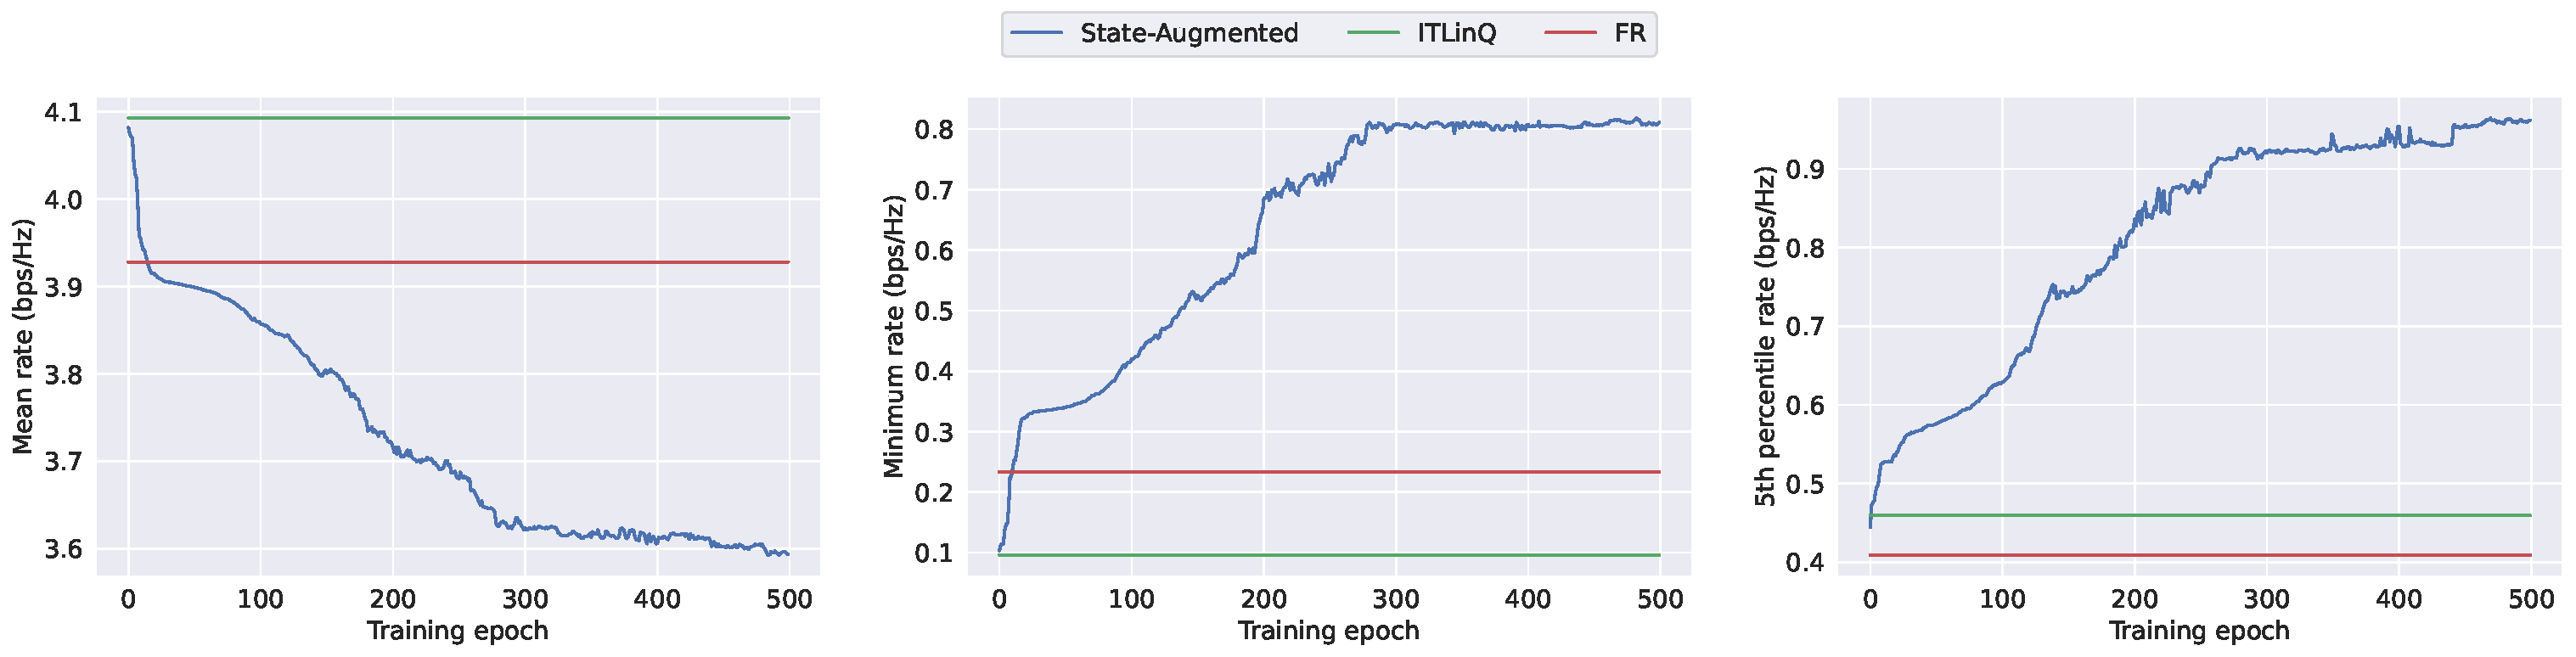
\includegraphics[width=\textwidth]{fig_convergence_singleConfig_m50_vardensity.pdf}
\caption{Convergence behavior of the proposed state-augmented RRM algorithm, and its comparison with the baseline methods for a \emph{single} network realization with $m=50$ transmitter-receiver pairs (variable-density scenario). Note that the baseline algorithms fail to achieve the minimum-rate requirement of $f_{\min}=0.6$, while our proposed method is able to satisfy the constraints for all $50$ users.
}
\label{fig:convergence_singleConfig_m50_vardensity}
\end{figure*}


\begin{figure*}[h]
\centering
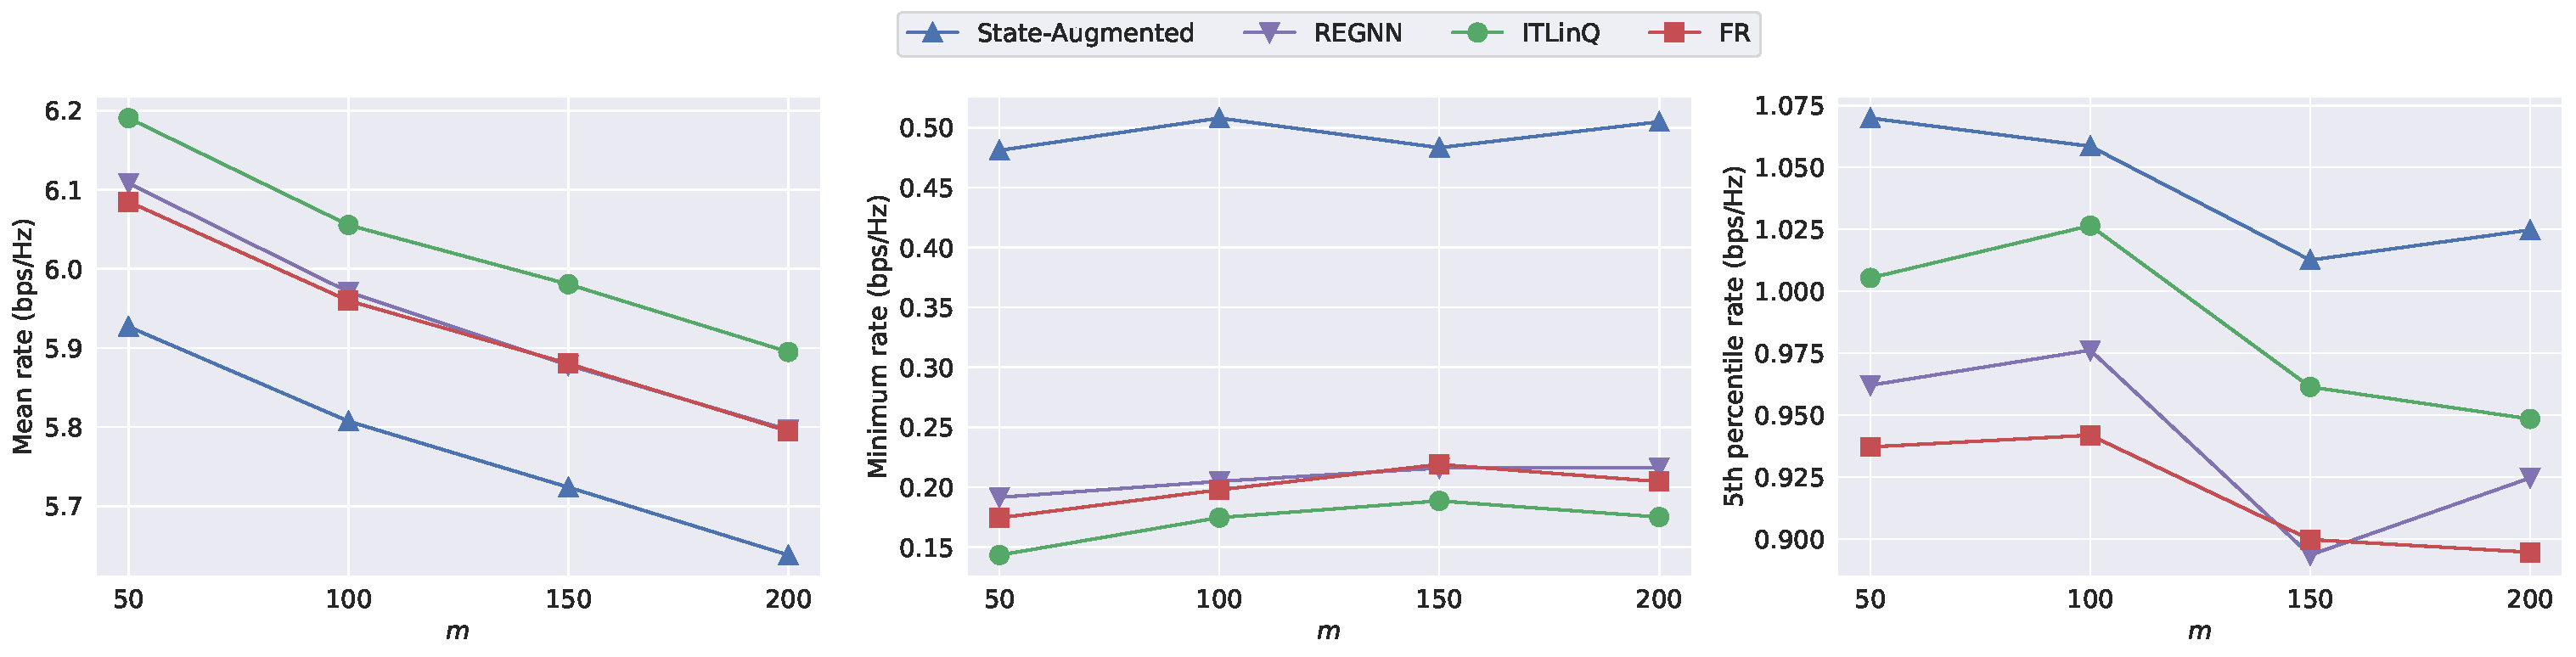
\includegraphics[width=\textwidth]{fig_scalability_fixed_density.pdf}
\caption{Performance comparison of the proposed state-augmented RRM algorithm against baseline methods in the fixed-density scenario for networks with $m\in\{50,100,150,200\}$ transmitter-receiver pairs.}
\label{fig:scalability_fixed_density}
\end{figure*}

\subsection{Experimental Results}\label{sec:exp_results}
We generate networks with $m$ transmitter-receiver pairs, located randomly within a square network area of side length $R$. We drop the transmitters uniformly at random within the network area, while ensuring a minimum distance of $75$m between each pair of them. Afterwards, for each transmitter, we drop its associated receiver uniformly at random within an annulus around the transmitter, with inner and outer radii of $10$m and $50$m, respectively. To control the network density, we consider the following two scenarios to determine the network area size:
\begin{itemize}
    \item \textbf{Fixed Density:} We set $R = \sqrt{m / 20} \times 2$km to keep the density constant (at $5$ users/km$^2$).
    \item \textbf{Variable Density:} We set $R=2$km, implying that the network density increases with $m$.
\end{itemize}
In both cases, and for all values of $m$, we set $f_{\min} = 0.6$bps/Hz, $T_0=5$, and $T=100$. We consider both large-scale and small-scale fading for the channel model. The large-scale fading follows a dual-slope path-loss model similar to~\cite{zhang2015downlink,andrews2016we,naderializadeh2022learning} alongside a $7$dB log-normal shadowing. Moreover, the small-scale fading models channel variations across different time steps following a Rayleigh distribution with a pedestrian speed of $1$m/s~\cite{li2002simulation}. We set the maximum transmit power to $P_{\max}=10$dBm, and the noise variance to $N=-104$dBm (due to the $10$MHz bandwidth and noise power spectral density of $-174$dBm/Hz).

We use a $3$-layer GNN with $F_1=F_2=64$, where the first two layers are based on the local extremum operator proposed in~\cite{ranjan2020asap}, while the last layer entails a linear projection (together with the mapping in~\eqref{eq:final_power_levels_GNN}). We set the primal and dual learning rates to $\eta_{\bbphi} = 10^{-1} / m$ and $\eta_{\bbmu} = 20$, respectively, and we set the batch size to $B=128$. For each value of $m$, we generate a total of $256$ training samples and $128$ samples for evaluation, where each sample refers to a realization of the transmitter/receiver locations (and the large-scale fading), alongside the small-scale fading random process. We set the normalization factor for edge weights at time step $t$ to $Z_t = \left\|\log\left(P_{\max}|\bbH_t|^2 / N\right)\right\|_2$. Except for the case of Section~\ref{sec:single_network} below, we run training for $100$ epochs, and we draw the dual variables during training randomly from the $U(0,1)$ distribution.

\urlstyle{tt}
As baselines, we compare the performance of our proposed method against three baselines: i) Full reuse (FR), where every transmitter uses $P_{\max}$; ii) Information-theoretic link scheduling (ITLinQ)~\cite{naderializadeh2014itlinq}, and iii) random-edge graph neural networks (REGNN)~\cite{eisen2020optimal}.\footnote{For a fair comparison with~\cite{eisen2020optimal}, we use the same exact GNN structure and hyperparameters as for our method to implement the REGNN method.} We would like to point out that, while the REGNN baseline allows the consideration of minimum-rate constraints, the first two baselines (i.e., FR and ITLinQ) are not able to handle such per-user requirements. In what follows, we primarily report the results in terms of three separate metrics, namely the mean rate, minimum rate (discarding the bottom 1\% of user rates as outliers), and the 5\textsuperscript{th} percentile rate, evaluated over the test configurations.\footnote{Our code is available at \url{https://github.com/navid-naderi/StateAugmented_RRM_GNN}.}




\begin{figure*}[h]
\centering
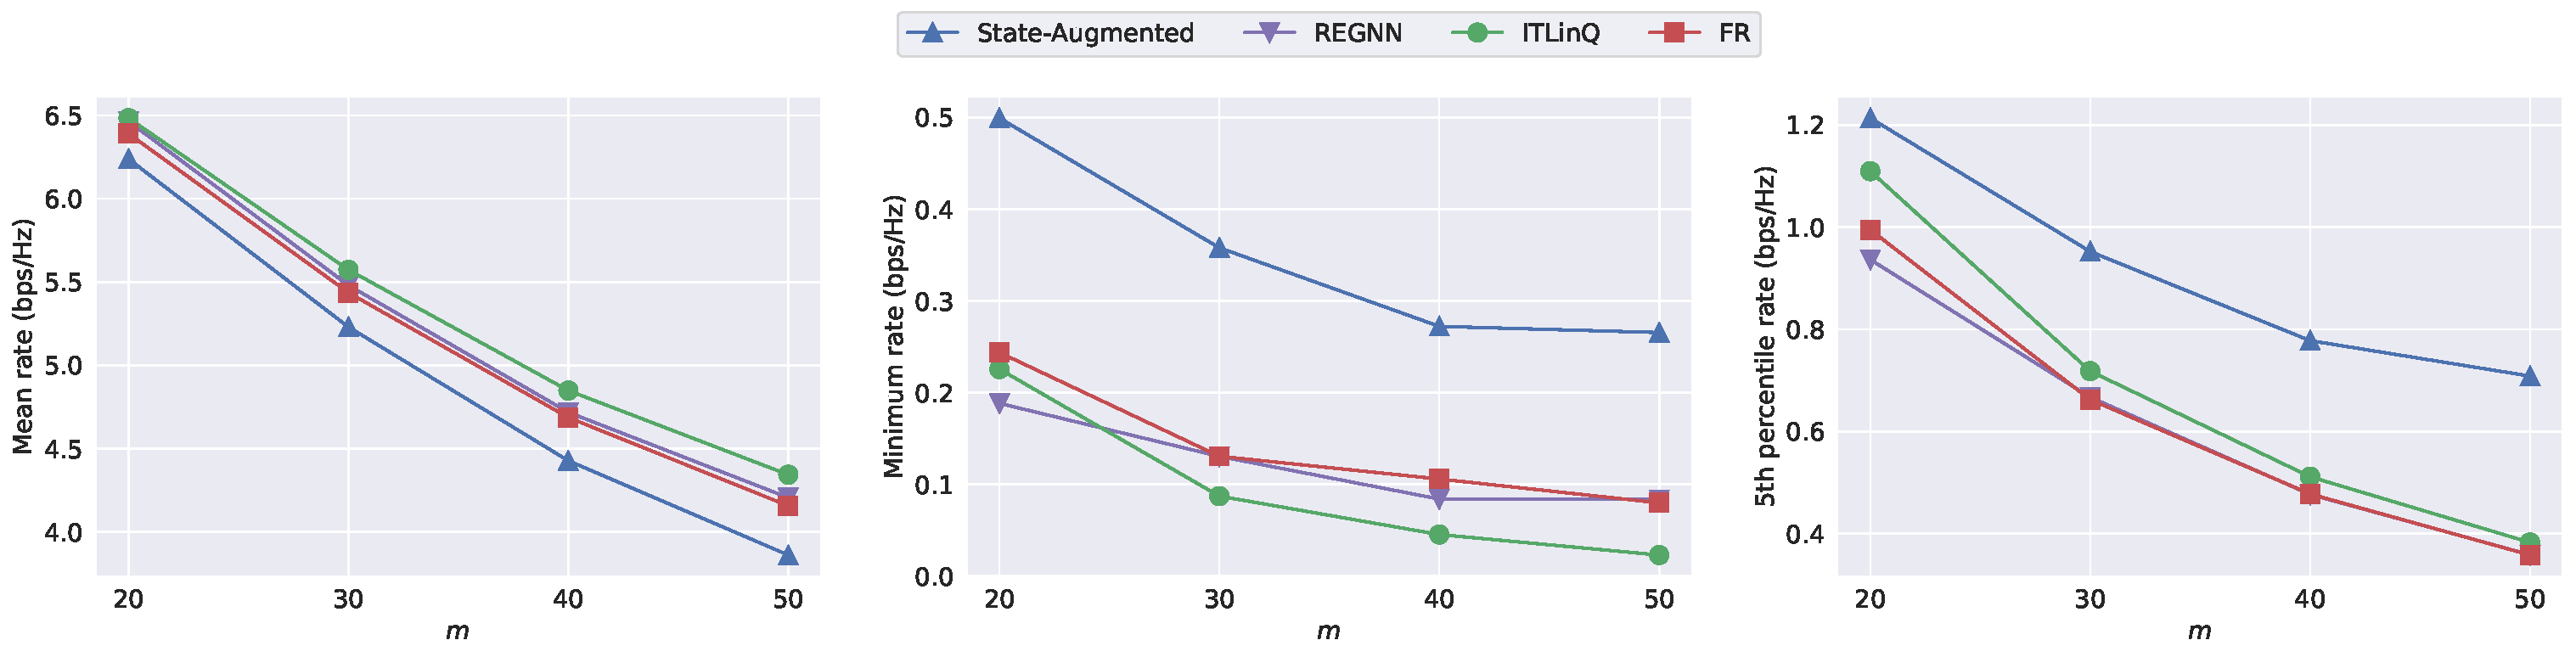
\includegraphics[width=\textwidth]{fig_scalability_variable_density.pdf}
\caption{Performance comparison of the proposed state-augmented RRM algorithm against baseline methods in the variable-density scenario for networks with $m\in\{20, 30, 40, 50\}$ transmitter-receiver pairs.}
\label{fig:scalability_variable_density}
\end{figure*}


\begin{figure*}[t!]
    \centering
    \begin{subfigure}[t]{0.5\textwidth}
        \centering
        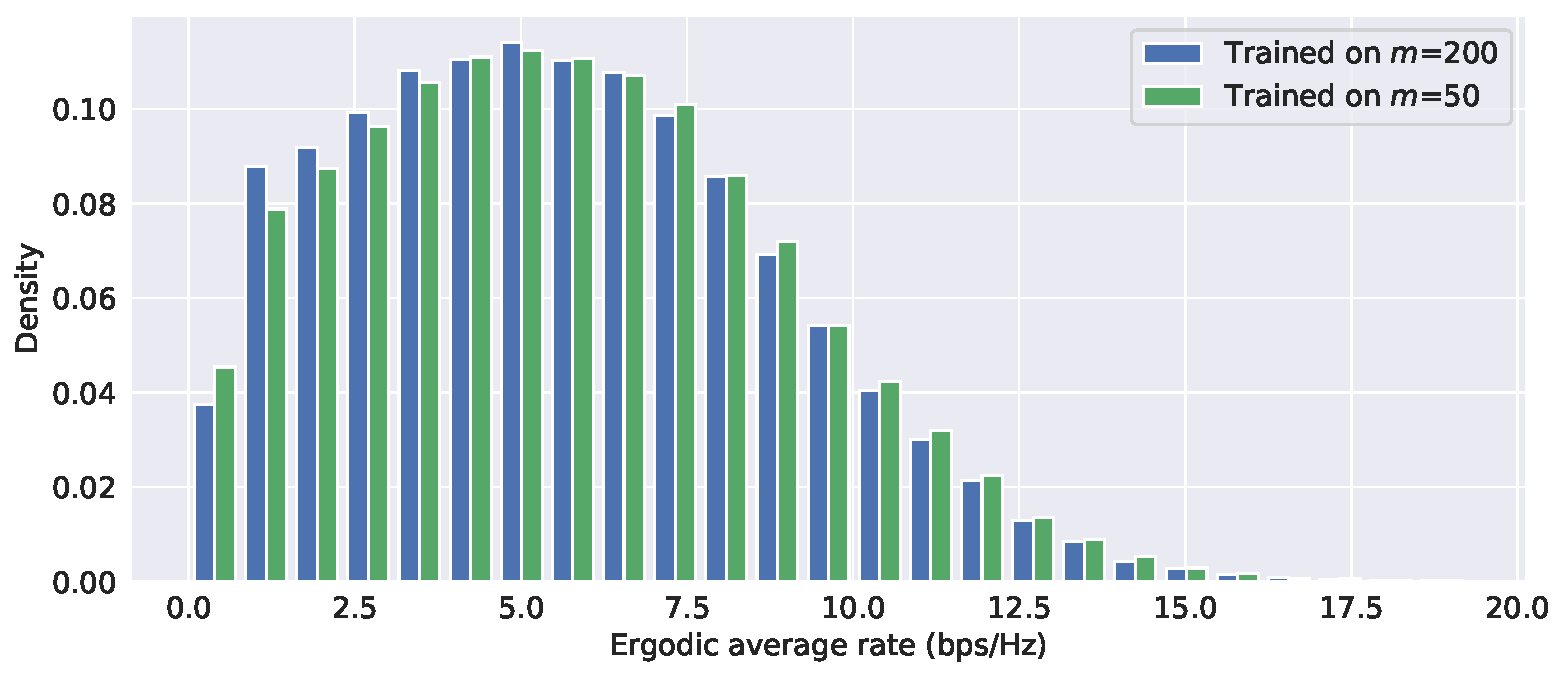
\includegraphics[width=.95\textwidth]{fig_transfer_fixed_density_50To200.pdf}
        \caption{\hspace*{-.25in}}
        \label{fig:transfer_fixed_density_50To200}
    \end{subfigure}%
    \hfill
    \begin{subfigure}[t]{0.5\textwidth}
        \centering
        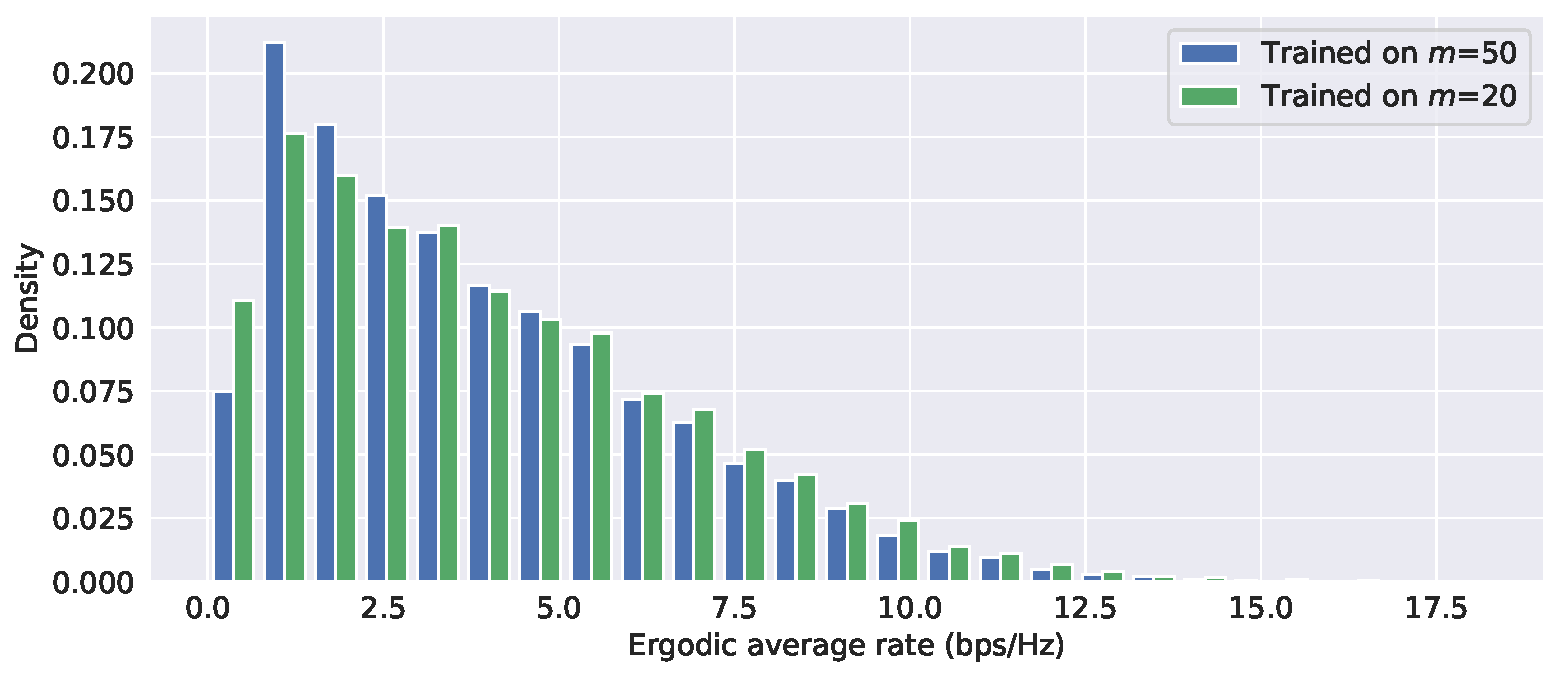
\includegraphics[width=.95\textwidth]{fig_transfer_variable_density_20To50.pdf}
        \caption{\hspace*{-.25in}}
        \label{fig:transfer_variable_density_20To50}
    \end{subfigure}%
    \caption{Transferability of the proposed state-augmented RRM procedure, shown as the histogram of ergodic average rates, for the (a) fixed-density scenario, evaluated on samples with $m=200$, and (b) variable-density scenario, evaluated on samples with $m=50$.}
    \label{fig:transferability}
\end{figure*}

\begin{figure*}[h]
\centering
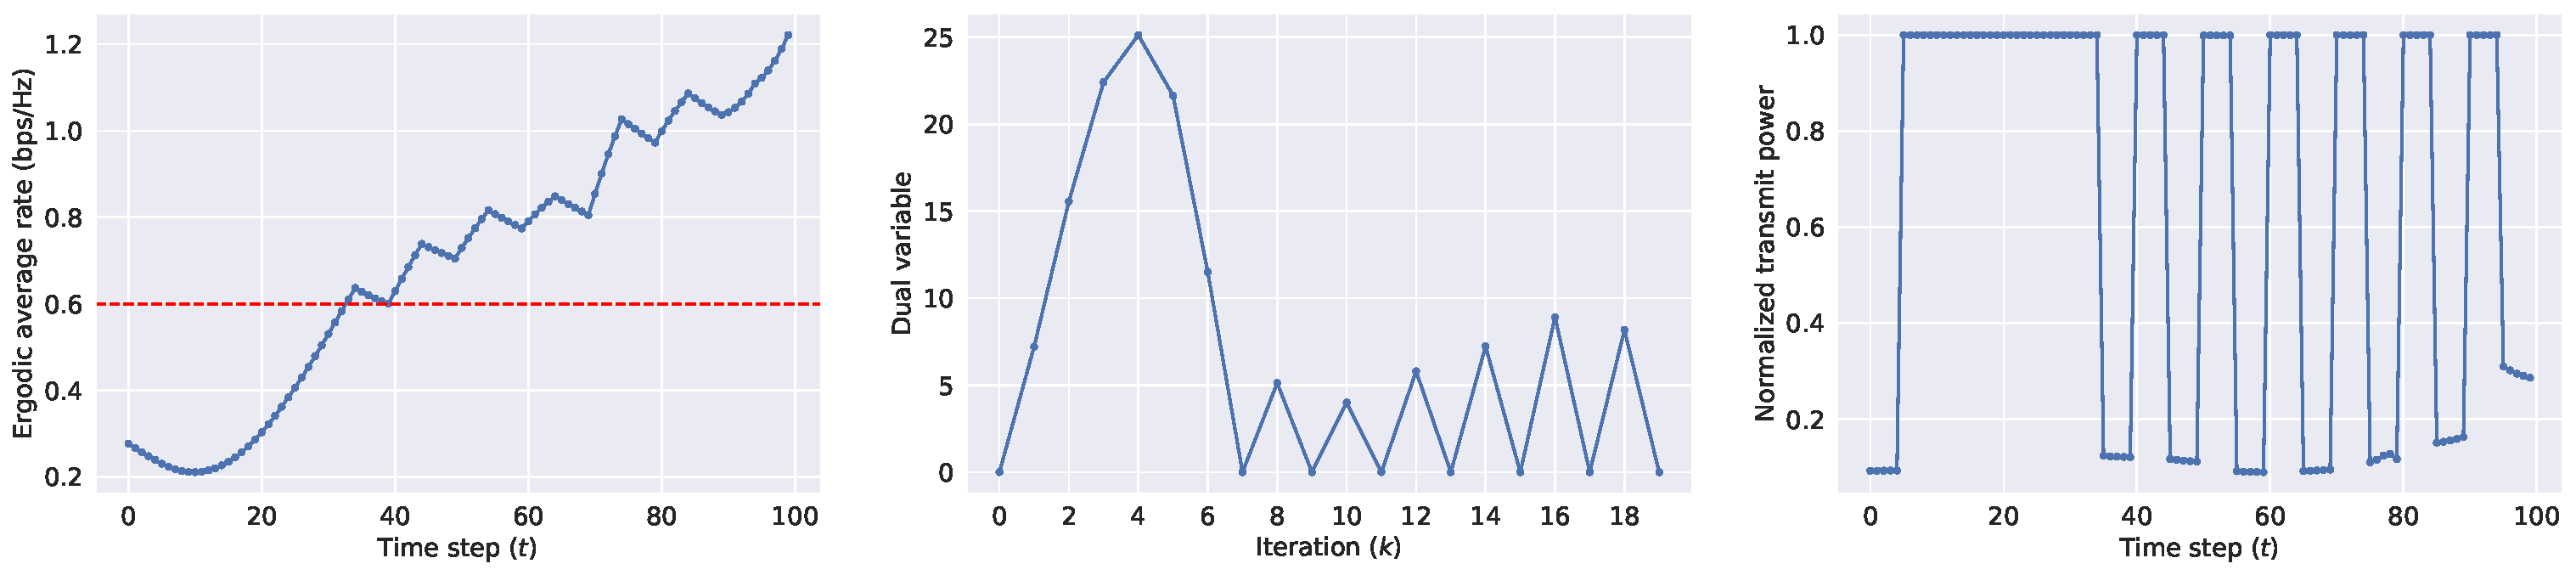
\includegraphics[width=\textwidth]{fig_policy_switching_m50_vardensity.pdf}
\caption{Evolution of the ergodic average rate (left), dual variable (middle), and normalized transmit power level (right) for an example user in a network with $m=50$ transmitter-receiver pairs (for the variable-density scenario). The dashed line in the left plot represents the minimum-rate requirement, i.e., $f_{\min}=0.6$.}
\label{fig:policy_switching_m50_vardensity}
\end{figure*}

\begin{figure}[h]
\centering
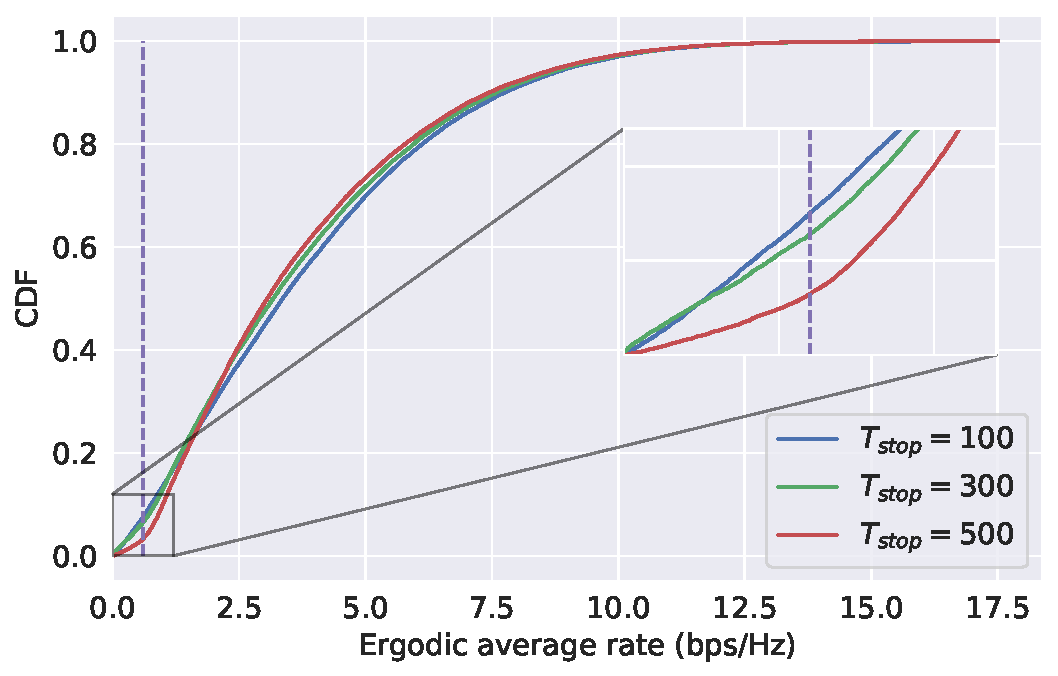
\includegraphics[width=.95\columnwidth]{fig_early_stopping_m50_vardensity_T500.pdf}
\caption{Impact of the early stopping of the dual descent updates on users' ergodic average rates in networks with $m=50$ transmitter-receiver pairs (for the variable-density scenario). The dashed line represents the minimum-rate requirement, i.e., $f_{\min}=0.6$.}
\label{fig:early_stopping_m50_vardensity_T500}
\end{figure}

% \begin{figure*}[h]
% \centering
% \includegraphics[width=\textwidth]{figs/impactoffmin_m6_T0_5.pdf}
% \caption{Impact of the minimum-rate constraint lower bound, $f_{\min}$, on the performance achieved by the proposed state-augmented RRM algorithm in networks with $m=6$ transmitter-receiver pairs (for the variable-density scenario).}
% \label{fig:impactoffmin_m6_T0_5}
% \end{figure*}


\subsubsection{Single Network Realization}\label{sec:single_network}
Figure~\ref{fig:convergence_singleConfig_m50_vardensity} shows the performance of our proposed method against the baselines for a \emph{single} network realization with $m=50$ users (in the variable-density scenario). For this specific experiment, we continue training for $500$ epochs, and decay the primal learning rate by $0.5$ every $100$ epochs. At the end of each training epoch, we evaluate the RRM algorithm on the same realization that is used for training. As the figure shows, our proposed state-augmented RRM algorithm considerably gains over the baseline algorithms in terms of the minimum and 5\textsuperscript{th} percentile rates, managing to satisfy the minimum-rate requirements for all users at the expense of a smaller achieved mean rate.

\subsubsection{Scalability}
Here, we assess the performance of the the proposed algorithm in \emph{families} of networks with different numbers of users, where the policies trained on samples with a specific value of $m$ are evaluated on test samples with the same value of $m$. Figures~\ref{fig:scalability_fixed_density} and~\ref{fig:scalability_variable_density} compare the performance of our proposed method with the baseline algorithms in the fixed-density and variable-density scenarios, respectively. In both scenarios, thanks to the feasibility guarantees of our proposed method for the per-user minimum-rate constraints, our method significantly outperforms the baseline methods in terms of the minimum rate and the 5\textsuperscript{th} percentile rate. This, however, comes at the cost of a slightly lower mean rate. Note that such a scalability is due to the size-invariant property of GNN-based parameterizations (where the number of parameters is fixed regardless of the graph size), as opposed to other parameterizations, such as multi-layer perceptrons (i.e., fully-connected neural networks).

\subsubsection{Transferability to Unseen Network Sizes}
Another upside of the size-invariance property of GNNs is that they can be evaluated on graph sizes not encountered throughout the training process. Figure~\ref{fig:transfer_fixed_density_50To200} shows the histogram of user ergodic average rates under our proposed algorithm in test networks of size $m=200$ (fixed-density scenario) using two GNNs: one trained on samples with $m=200$ and the other trained on samples with $m=50$. Moreover, Figure~\ref{fig:transfer_variable_density_20To50} shows a similar histogram for the variable-density scenario, where GNNs trained on samples with $m=50$ and $m=20$ are evaluated on test samples with $m=50$. As the figures show, in both cases, the trained GNNs provide excellent transferability to larger network sizes, achieving user rates that are similar to the GNNs without the train/test mismatch. Moreover, as expected, the transferred performance is more desirable in the fixed-density scenario than the variable-density scenario, as the channel statistics mostly remain similar in the former case, while in the latter case, the network becomes more interference-limited as $m$ grows.


\subsubsection{Policy Switching}
Figure~\ref{fig:policy_switching_m50_vardensity} shows what an example receiver experiences over the course of the $T=100$ time steps in a test network with $m=50$ transmitter-receiver pairs (for the variable-density scenario) once training is completed. Letting $i$ denote the receiver index, at each time step $t$, we plot its ergodic average rate up to that time step (i.e., $\frac{1}{t} \sum_{\tau=1}^t f_i(\bbH_{\tau}, \bbp(\bbH_{\tau},\bbmu_{\lfloor \tau / T_0 \rfloor};\bbphi^{\star}))$), its dual variable at the corresponding iteration (i.e., $\mu_{i,\lfloor t / T_0 \rfloor}$), and the selected normalized transmit power of transmitter $i$ at that time step (i.e., $p_i(\bbH_t,\bbmu_{\lfloor t / T_0 \rfloor};\bbphi^{\star}) / P_{\max}$). As the figure shows, a \emph{policy switching} behavior occurs, where for the time steps in which the receiver's ergodic average rate is below $f_{\min}$, the dual variable increases, leading to the corresponding transmitter using full transmit power. Moreover, when the ergodic average rate exceeds $f_{\min}$, the transmitter uses an on-off pattern to maintain its receiver's high ergodic average rate, while minimizing the interference caused at other receivers. This shows why state-augmentation is crucial for the algorithm to be able to switch the policy if/when necessary, depending on the constraint violations over time. Indeed, neither the ``off'' policy ($p_i=0$) nor the ``on'' policy ($p_i=P_{\max}$) guarantees the satisfaction of the constraints by itself. However, the illustrated policy switching behavior in Figure~\ref{fig:policy_switching_m50_vardensity} is exactly what the transmitters need to show in order to be able to satisfy their constraints in the long run.

\subsubsection{Drawback of Early Stopping of Dual Descent Iterations}
As we mentioned in Section~\ref{sec:alg}, the feasibility and near-optimality of the RRM decisions depend on the fact that the dual descent iterations in~\eqref{eq:mu_dynamics_augmented} continue for the entire duration of the execution phase. This implies that such feasibility and near-optimality guarantees will not hold if the dual descent updates are stopped at a small, finite number of iterations. Figure~\ref{fig:early_stopping_m50_vardensity_T500} illustrates the empirical cumulative distribution function (CDF) of the user ergodic average rates in test networks with $m=50$ transmitter-receiver pairs (for the variable-density scenario), where the dual descent updates are stopped at a certain time step $T_{\text{stop}} \in \{100, 300, 500\}$. For the sake of this experiment, we expanded the execution time horizon to $T=500$ time steps. As the figure shows, early stopping of the dual variable updates leads to a larger fraction of users violating their minimum-rate requirements. Quite interestingly, such an early stopping provides an equivalent way of implementing the regular primal-dual REGNN method in~\cite{eisen2020optimal}.

\subsubsection{Inference Computational Complexity}
The size-invariance property of the GNNs implies that the number of GNN parameters does not depend on the underlying graph size on which the GNN is operating. However, using GNNs on larger graph sizes naturally leads to a higher computational complexity. Figure~\ref{fig:inference_time_vs_m} shows the average inference time (on CPU) for graphs corresponding to networks with $m\in[20, 200]$ transmitter-receiver pairs. Note that, in practice, the inference time can effectively be reduced by parallelizing computations on GPU hardware architectures.

\begin{figure}[t!]
\centering
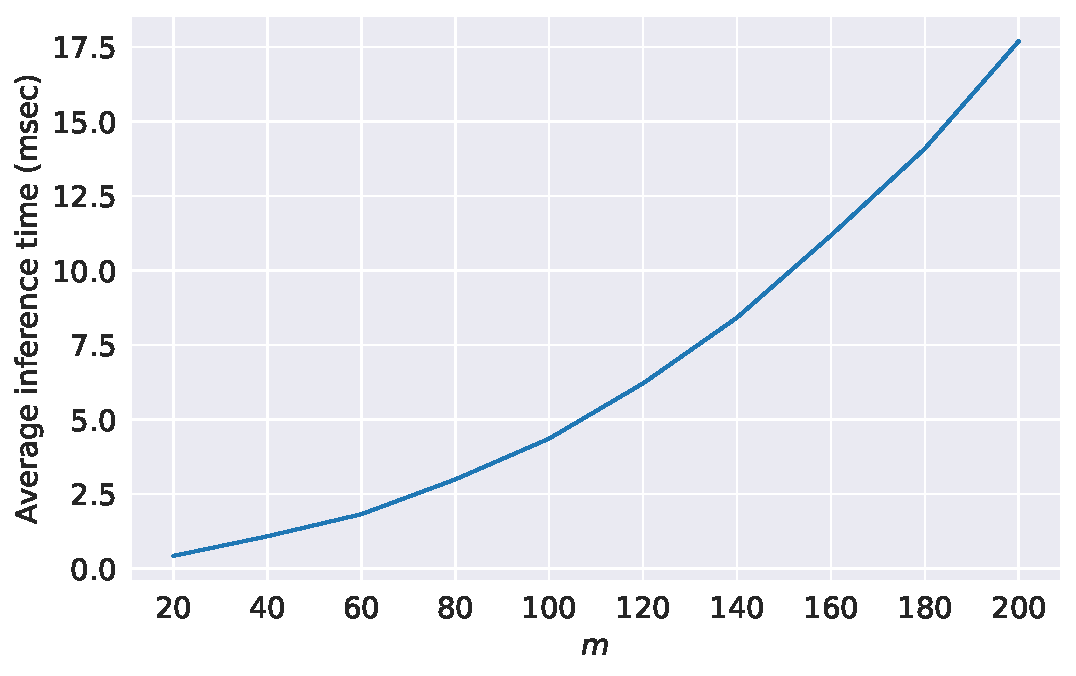
\includegraphics[width=.97\columnwidth]{fig_inference_time_vs_m.pdf}
\caption{Average inference time (on a CPU hardware architecture) for networks with $m\in[20,200]$ transmitter-receiver pairs.}
\label{fig:inference_time_vs_m}
\end{figure}


% \subsubsection{Impact of the Minimum-Rate Constraint Lower Bounds}
% In all our experiments, we set the lower bounds for the minimum-rate constraints, i.e., $f_{\min}$ to $\frac{3}{4}$. This resulted in RRM decisions that attempted to satisfy relatively strict minimum-rate constraints for almost all network realizations, which came at the cost of lower mean rates as compared to baseline methods. Figure~\ref{fig:impactoffmin_m6_T0_5} demonstrates the impact of the constraint lower bounds $f_{\min} \in \left\{\frac{1}{4}, \frac{1}{2}, \frac{3}{4}, 1\right\}$ on the performance of the proposed state-augmented RRM algorithm when trained and evaluated on networks with $m=6$ transmitter-receiver pairs (in the variable-density scenario). As the figure shows, tuning $f_{\min}$ reveals the trade-off between the average and worst-case performance of users across all network realizations. Finding the best minimum-rate constraint lower bound is a non-trivial problem, and it has also been shown that this bound can be tuned adaptively based on each specific network realization through the introduction of learnable slack parameters~\cite{naderializadeh2020wireless, naderializadeh2022learning, naderializadeh2022adaptive}. We leave the incorporation of adaptive minimum-rate constraints into state-augmented RRM algorithms as future work.

\section{Concluding Remarks}\label{sec:conclusion}
We considered the problem of resource allocation in wireless network, termed radio resource management (RRM), in which the goal is to maximize a network-wide utility subject to constraints on the long-term average performance of the network users. We showed how parameterized dual-based RRM policies can lead to feasible and near-optimal solutions, but suffer from multiple challenges, including that they need to be run for an infinite number of time steps and the model parameters have to be optimized for any given set of dual variables at every time step. To mitigate these challenges, we proposed a state-augmented RRM algorithm, which revises the parameterization to take as input the network state, as well as the dual variable at each step, and produce as output the RRM decisions. We showed that for near-universal parameterizations, the proposed method also leads to feasible and near-optimal sequences of RRM decisions. Using graph neural network (GNN) architectures to parameterize the state-augmented RRM policy, we also demonstrated, via a set of numerical experiments, that the proposed method provides scalable and transferable wireless power control solutions that outperform baseline algorithms.




\appendices
\section{Proof of Theorem~\ref{thm:main}}\label{appx:proof}
\allowdisplaybreaks

The arguments used in the proof of Theorem~\ref{thm:main} follow similar steps to those in~\cite{calvo2021state}, with some minor differences specific to our problem formulation, as outlined in Remark~\ref{remark:proof_diff}. We, therefore, include the complete proof here for the paper to be self-complete.% there are differences with prior proofs, specific to our problem formulation, that require us to include the complete proof here.

\subsection{Tightness of The Sequence of Dual Variable Probability Measures}\label{appx:proof_tightness}
We start by proving that the sequence of dual variable probability measures, i.e., $\{p(\bbmu_k|\bbmu_0)\}_{k}$, is tight in the following lemma.

\begin{lemma}
For any $\delta > 0$, there exists a compact set $\ccalA_{\delta}$ such that for every $k \geq 0$, we have $\mathsf{Pr}[\bbmu_k \in \ccalA_{\delta}] > 1 - \delta$.
\end{lemma}

\begin{proof}
Define the dual function, $d(\bbmu)$ as
\begin{align}\label{eq:def_dual_function}
d(\bbmu) = \max_{\bbtheta\in\bbTheta} \ccalL(\bbtheta, \bbmu),
\end{align}
and consider the following set:
\begin{align}\label{eq:def_C}
\ccalC = \left\{\bbmu \in \reals_+^c : d(\bbmu) - P^{\star} \leq \frac{c\eta_{\bbmu}G^2}{2} \right\}.
\end{align}
Now, let
\begin{align}
\ccalA_{\delta} = \ccalB_{\delta} \cup \left(\ccalC \oplus \ccalS_{\sqrt{c\eta_{\bbmu}^2 G^2}}\right),
\end{align}
where $\oplus$ denotes Minkowski sum, $\ccalS_r$ denotes a ball centered at the origin with radius $r\geq0$, and $\ccalB_{\delta}$ is defined as
\begin{align}
\ccalB_{\delta} = \left\{\bbmu \in \reals_+^c : \frac{\| \bbmu - \bbmu^{\star} \|}{\| \bbmu_0 - \bbmu^{\star}\|} \leq \frac{1}{\delta} \right\},
\end{align}
with $\bbmu^{\star}$ representing the optimal set of dual variables. Then, we have
\begin{align}
&\mathsf{Pr}[\bbmu_k \in \ccalA_{\delta}] \nonumber \\
& = \mathsf{Pr}\left[\bbmu_k \in \ccalB_{\delta} \cup \left(\ccalC \oplus \ccalS_{\sqrt{c\eta_{\bbmu}^2 G^2}}\right) \right] \\
& = \underbrace{\mathsf{Pr}\left[\bbmu_k \in \ccalB_{\delta} \cup \left(\ccalC \oplus \ccalS_{\sqrt{c\eta_{\bbmu}^2 G^2}}\right) \middle| \bbmu_{k-1}\in\ccalC \right]}_{\overset{(a)}{=}1} \cdot \ p \nonumber \\
& \quad + \underbrace{\mathsf{Pr}\left[\bbmu_k \in \ccalB_{\delta} \cup \left(\ccalC \oplus \ccalS_{\sqrt{c\eta_{\bbmu}^2 G^2}}\right) \middle| \bbmu_{k-1}\in\ccalC^c \right]}_{\geq \mathsf{Pr}\left[\bbmu_k \in \ccalB_{\delta}  \middle| \bbmu_{k-1}\in\ccalC^c \right]} \cdot \ (1-p) \nonumber \\
& \geq \mathsf{Pr}\left[\bbmu_k \in \ccalB_{\delta}  \middle| \bbmu_{k-1}\in\ccalC^c \right] \\
& = \mathsf{Pr}\left[\frac{\| \bbmu_k - \bbmu^{\star} \|}{\| \bbmu_0 - \bbmu^{\star}\|} \leq \frac{1}{\delta}  \middle| \bbmu_{k-1}\in\ccalC^c \right] \\
& \geq 1 - \left( \frac{\E\left[\| \bbmu_k - \bbmu^{\star} \| \middle| \bbmu_{k-1}\in\ccalC^c\right]}{\| \bbmu_0 - \bbmu^{\star}\|} \right) \delta,
\end{align}
where $p=\mathsf{Pr}\left[\bbmu_{k-1}\in\ccalC \right]$, (a) is true due to the dual dynamics in~\eqref{eq:mu_dynamics} and the fact that the change between $\bbmu_{k-1}$ and $\bbmu_k$ is upper bounded in norm by $\sqrt{c\eta_{\bbmu}^2 G^2}$, and the last inequality is due to conditional Markov's inequality. Therefore, to complete the proof, it suffices to show that (i)
\begin{align}\label{eq:bounded_conditional_difference_norm_muk}
\E\left[\| \bbmu_k - \bbmu^{\star} \| \middle| \bbmu_{k-1}\in\ccalC^c\right] < \| \bbmu_0 - \bbmu^{\star}\|,
\end{align}
and (ii) that $\ccalA_{\delta}$ is compact.

\noindent\textbf{Proof of~\eqref{eq:bounded_conditional_difference_norm_muk}.}
Let $\Delta_{\bbmu_{k-1}}$ be defined as
\begin{align}
\Delta_{\bbmu_{k-1}} \coloneqq \bbg\left( \frac{1}{T_0} \sum_{t=(k-1)T_0}^{kT_0-1} \bbf(\bbH_{t}, \bbp(\bbH_{t};\bbtheta_{k-1})) \right).
\end{align}
Then, from the dual dynamics in~\eqref{eq:mu_dynamics}, we have
\begin{align*}
&\|\bbmu_{k} - \bbmu^{\star}\|^2 \\
&\leq \|\bbmu_{k-1} - \bbmu^{\star} - \eta_{\bbmu} \Delta_{\bbmu_{k-1}} \|^2 \\
&= \|\bbmu_{k-1} - \bbmu^{\star}  \|^2 + \eta_{\bbmu}^2 \|\Delta_{\bbmu_{k-1}} \|^2 \nonumber \\
&\quad - 2\eta_{\bbmu} (\bbmu_{k-1} - \bbmu^{\star})^T \Delta_{\bbmu_{k-1}} \\
&\leq \|\bbmu_{k-1} - \bbmu^{\star}  \|^2 + c \eta_{\bbmu}^2 G^2 - 2\eta_{\bbmu} (\bbmu_{k-1} - \bbmu^{\star})^T \Delta_{\bbmu_{k-1}},
\end{align*}
where the last inequality follows from the fact that for any $i\in\{1,\dots,c\}$, we assume $|g_i\left(\cdot\right)|\leq G$. Taking the expectation of both sides conditioned on $\bbmu_{k-1}$, we have
\begin{align}
&\E\left[\|\bbmu_{k} - \bbmu^{\star}\|^2 \middle| \bbmu_{k-1}\right] \nonumber\\
&\leq \|\bbmu_{k-1} - \bbmu^{\star}  \|^2 + c \eta_{\bbmu}^2 G^2 \nonumber \\
&\quad - 2\eta_{\bbmu} (\bbmu_{k-1} - \bbmu^{\star})^T \E\left[\Delta_{\bbmu_{k-1}}\middle| \bbmu_{k-1}\right]\\
&\leq \|\bbmu_{k-1} - \bbmu^{\star}  \|^2 + c \eta_{\bbmu}^2 G^2 - 2\eta_{\bbmu} (d(\bbmu_{k-1}) - d(\bbmu^{\star}))\label{eq:subgradient}\\
&= \|\bbmu_{k-1} - \bbmu^{\star}  \|^2 + c \eta_{\bbmu}^2 G^2 - 2\eta_{\bbmu} (d(\bbmu_{k-1}) - P^{\star}),\label{eq:pre_C_bound}
\end{align}
where~\eqref{eq:subgradient} follows from the fact that $\Delta_{\bbmu_{k-1}}$ is a subgradient of the dual function~\cite{danskin2012theory}, leading to the inequality $(\bbmu_{k-1} - \bbmu^{\star})^T \E\left[\Delta_{\bbmu_{k-1}}\middle| \bbmu_{k-1}\right] \geq d(\bbmu_{k-1}) - d(\bbmu^{\star})$ thanks to the dual function being convex~\cite{boyd2004convex}. Now, combining the fact that $\bbmu_{k-1}\in\ccalC^c$ with the definition of $\ccalC$ in~\eqref{eq:def_C}, we can continue~\eqref{eq:pre_C_bound} as
\begin{align}
\E\left[\|\bbmu_{k} - \bbmu^{\star}\|^2 \middle| \bbmu_{k-1}\in\ccalC^c\right]
&< \|\bbmu_{k-1} - \bbmu^{\star}\|^2 \\
&< \|\bbmu_{0} - \bbmu^{\star}\|^2,
\end{align}
with the last inequality following from recursion.


\noindent\textbf{Proof of Compactness of $\ccalA_{\delta}$.} Since the Minkowski sum of two compact sets is compact, and also the union of two compact sets is compact, it suffices to show that the set $\ccalC$ is compact.

Given the definition of the dual function in~\eqref{eq:def_dual_function}, for any set of model parameters $\bbtheta\in\bbTheta$ and any set of dual variables $\bbmu\in\reals_+^c$, we have
\begin{align}
d(\bbmu) &\geq \mathcal{U}\left( \frac{1}{T} \sum_{t=0}^{T-1} \bbf(\bbH_t, \bbp(\bbH_t;\bbtheta)) \right)\nonumber \\
   &\qquad\qquad+ \bbmu^T \bbg\left( \frac{1}{T} \sum_{t=0}^{T-1} \bbf(\bbH_t, \bbp(\bbH_t;\bbtheta)) \right)
\end{align}
Now, replacing $\bbtheta$ with the strictly-feasible set of model parameters $\hat{\bbtheta}$ considered in Theorem~\ref{thm:main}, we can write
\begin{align}
d(\bbmu) &\geq \mathcal{U}\left( \frac{1}{T} \sum_{t=0}^{T-1} \bbf(\bbH_t, \bbp(\bbH_t;\hat{\bbtheta})) \right)\nonumber \\
   &\qquad\qquad+ \bbmu^T \bbg\left( \frac{1}{T} \sum_{t=0}^{T-1} \bbf(\bbH_t, \bbp(\bbH_t;\hat{\bbtheta})) \right)\\
&\geq \mathcal{U}\left( \frac{1}{T} \sum_{t=0}^{T-1} \bbf(\bbH_t, \bbp(\bbH_t;\hat{\bbtheta})) \right) + G' \| \bbmu \|_1.\label{eq:dual_upper_bound}
\end{align}
Now, for any $\bbmu\in\ccalC$, according to the definition in~\eqref{eq:def_C}, the bound in~\eqref{eq:dual_upper_bound} leads to
\begin{align}
P^{\star} + \frac{c\eta_{\bbmu}G^2}{2}  \geq \mathcal{U}\left( \frac{1}{T} \sum_{t=0}^{T-1} \bbf(\bbH_t, \bbp(\bbH_t;\hat{\bbtheta})) \right) + G' \| \bbmu \|_1,
\end{align}
implying that $\bbmu$ belongs to the following ball,
\begin{align}
\| \bbmu \|_1 \leq \frac{P^{\star} + \frac{c\eta_{\bbmu}G^2}{2} - \mathcal{U}\left( \frac{1}{T} \sum_{t=0}^{T-1} \bbf(\bbH_t, \bbp(\bbH_t;\hat{\bbtheta})) \right)}{G'},
\end{align}
hence completing the proof.


\end{proof}

\subsection{Proof of Feasibility in~\eqref{eq:thm_feasibility}}\label{appx:proof_feasibility}

From the dual dynamics in~\eqref{eq:mu_dynamics}, we have
\begin{align}\label{eq:mu_inequality}
% \bbmu_{T+1} &\geq \bbmu_T - \eta_{\bbmu} \bbg\left(  \bbf(\bbH_T, \bbp(\bbH_T;\bbtheta_T)) \right).
\bbmu_{K} &\geq \bbmu_{K-1} - \eta_{\bbmu} \bbg\left( \frac{1}{T_0} \sum_{t=(K-1)T_0}^{KT_0-1} \bbf(\bbH_{t}, \bbp(\bbH_{t};\bbtheta_{K-1})) \right)\hspace{-3pt}.
\end{align}
Using the inequality in~\eqref{eq:mu_inequality} recursively yields
% \begin{align}
% \bbmu_{T+1} &\geq \bbmu_1 - \eta_{\bbmu} \sum_{t=1}^T \bbg\left(  \bbf(\bbH_t, \bbp(\bbH_t;\bbtheta_t)) \right) \\
% &= \bbmu_1 - T \eta_{\bbmu} \left(\frac{1}{T} \sum_{t=1}^T  \bbg\left(  \bbf(\bbH_t, \bbp(\bbH_t;\bbtheta_t)) \right)\right) \\
% &\geq \bbmu_1 - T \eta_{\bbmu}  \bbg\left( \frac{1}{T} \sum_{t=1}^T  \bbf(\bbH_t, \bbp(\bbH_t;\bbtheta_t)) \right),
% \end{align}
\begin{align*}
&\bbmu_{K} \nonumber \\
&\geq \bbmu_0 - \eta_{\bbmu} \sum_{k=0}^{K-1} \bbg\left( \frac{1}{T_0} \sum_{t=kT_0}^{(k+1)T_0-1} \bbf(\bbH_{t}, \bbp(\bbH_{t};\bbtheta_k)) \right) \nonumber \\
&= \bbmu_0 - K\eta_{\bbmu} \cdot \frac{1}{K}\hspace{-3pt}\sum_{k=0}^{K-1} \bbg\left( \frac{1}{T_0} \sum_{t=kT_0}^{(k+1)T_0-1} \bbf(\bbH_{t}, \bbp(\bbH_{t};\bbtheta_k)) \right) \nonumber \\
&\geq \bbmu_0 - K\eta_{\bbmu} \bbg\left( \frac{1}{KT_0} \sum_{t=0}^{KT_0-1} \bbf(\bbH_t, \bbp(\bbH_t;\bbtheta_{\lfloor t/T_0 \rfloor})) \right),
\end{align*}
where the last inequality follows from the concavity of $\bbg(\cdot)$. Therefore, we have
% \begin{align}\label{eq:muT+1_vs_mu1}
% &\limsup_{T\to\infty}\bbmu_{T+1}  \nonumber\\ 
% &\geq \bbmu_1 - \eta_{\bbmu} \liminf_{T\to\infty} T \bbg\left( \frac{1}{T} \sum_{t=1}^T  \bbf(\bbH_t, \bbp(\bbH_t;\bbtheta_t)) \right).
% \end{align}
\begin{align}\label{eq:muT+1_vs_mu1}
&\limsup_{K\to\infty}\bbmu_{K+1}  \nonumber\\ 
&\geq \bbmu_0 - \eta_{\bbmu} \liminf_{K\to\infty} K \bbg\left( \frac{1}{T} \sum_{t=0}^{T-1} \bbf(\bbH_t, \bbp(\bbH_t;\bbtheta_{\lfloor t/T_0 \rfloor})) \right).
\end{align}
Now, assume by contradiction that one of the constraints in~\eqref{eq:thm_feasibility} is not satisfied. More precisely, assume there exists an index $i\in\{1,\dots,c\}$ and positive constants $\delta>0$ and $\beta\in(0,1)$ such that
\begin{align}\label{eq:contradiction_prob}
\mathsf{Pr}\left[\liminf_{T\to\infty} g_i\left( \frac{1}{T} \sum_{t=0}^{T-1} \bbf(\bbH_t, \bbp(\bbH_t;\bbtheta_{\lfloor t/T_0 \rfloor})) \right) \leq -\delta \right] = \beta.
\end{align}
This implies that with non-zero probability $\beta$, we would have
% \begin{align}
% &\limsup_{T\to\infty} \|\bbmu_{T+1}\|_1 \nonumber \\
% &\geq \limsup_{T\to\infty} \mu_{i,T+1}\label{eq:1_norm} \\
% &\geq \mu_{i,1} - \eta_{\bbmu} \liminf_{T\to\infty} T g_i\left( \frac{1}{T} \sum_{t=1}^T  \bbf(\bbH_t, \bbp(\bbH_t;\bbtheta_t)) \right)\label{eq:ith_bound} \\
% &\geq \mu_{i,1} + \eta_{\bbmu} \liminf_{T\to\infty} T \epsilon \label{eq:contradiction_prob_use} \\
% &= \infty,
% \end{align}
\begin{align}
&\limsup_{K\to\infty} \|\bbmu_{K}\|_1 \nonumber \\
&\geq \limsup_{K\to\infty} \mu_{i,K}\label{eq:1_norm} \\
&\geq \mu_{i,0} - \eta_{\bbmu} \liminf_{K\to\infty} K g_i\left( \frac{1}{T} \sum_{t=0}^{T-1} \bbf(\bbH_t, \bbp(\bbH_t;\bbtheta_{\lfloor t/T_0 \rfloor})) \right)\label{eq:ith_bound} \\
&\geq \mu_{i,0} + \eta_{\bbmu} \liminf_{K\to\infty} K \epsilon \label{eq:contradiction_prob_use} \\
&= \infty,
\end{align}
where~\eqref{eq:1_norm} follows from the definition of the $\ell_1$-norm% and the fact that $\mu_{i,T+1} \geq 0$
,~\eqref{eq:ith_bound} follows from the $i$\textsuperscript{th} inequality in~\eqref{eq:muT+1_vs_mu1}, and~\eqref{eq:contradiction_prob_use} follows from~\eqref{eq:contradiction_prob}. This contradicts the fact that the sequence of dual variable probabilities is tight, hence completing the proof.
\hfill$\square$


\subsection{Proof of Optimality in~\eqref{eq:thm_optimality}}


Given the dual dynamics in~\eqref{eq:mu_dynamics} and the fact that projection onto the non-negative orthant does not increase the $\ell_2$-norm, we have
\begin{align}
&\left\|\bbmu_{K+1}\right\|^2\nonumber\\
&\leq \left\|\bbmu_K - \eta_{\bbmu} \bbg\left( \frac{1}{T_0} \sum_{t=KT_0}^{(K+1)T_0-1} \bbf(\bbH_{t}, \bbp(\bbH_{t};\bbtheta_K)) \right) \right\|^2\label{eq:norm_dual_update}\\
&=\left\|\bbmu_K \right\|^2 + \eta_{\bbmu}^2 \left\| \bbg\left( \frac{1}{T_0} \sum_{t=KT_0}^{(K+1)T_0-1} \bbf(\bbH_{t}, \bbp(\bbH_{t};\bbtheta_K)) \right)\right\|^2 \nonumber \\
&~\quad- 2\eta_{\bbmu}\bbmu_K^T \bbg\left( \frac{1}{T_0} \sum_{t=KT_0}^{(K+1)T_0-1} \bbf(\bbH_{t}, \bbp(\bbH_{t};\bbtheta_K)) \right)\label{eq:norm_dual_square_expansion}\\
&\leq\left\|\bbmu_T\right\|^2 + c\eta_{\bbmu}^2 G^2  \nonumber \\
&~\quad - 2\eta_{\bbmu}\bbmu_K^T \bbg\left( \frac{1}{T_0} \sum_{t=KT_0}^{(K+1)T_0-1} \bbf(\bbH_{t}, \bbp(\bbH_{t};\bbtheta_K)) \right),\label{eq:g_bounded}
\end{align}
% Since $\left\|\bbmu_{T+1}\right\|^2 \geq 0$, expanding the squared norm on the right-hand side of~\eqref{eq:norm_dual_update} yields
% \begin{align}\label{eq:norm_dual_square_expansion}
% 0 &\leq \left\|\bbmu_T\right\|^2 + \eta_{\bbmu}^2 \left\| \bbg\left(  \bbf(\bbH_T, \bbp(\bbH_T, \bbmu_T;\bbtheta)) \right)\right\|^2 - 2\eta_{\bbmu}\bbmu_T^T \bbg\left(  \bbf(\bbH_T, \bbp(\bbH_T, \bbmu_T;\bbtheta)) \right) .
% \end{align}
%Since 
where the last inequality follows from the fact that for any $i\in\{1,\dots,c\}$, we assume $|g_i\left(\cdot\right)|\leq G$. Applying~\eqref{eq:g_bounded} recursively yields
\begin{align}
&\left\|\bbmu_{K+1}\right\|^2 \nonumber\\
&\leq \left\|\bbmu_0\right\|^2 + c\eta_{\bbmu}^2 K G^2  \nonumber \\
&~\quad - 2\eta_{\bbmu} \sum_{k=0}^{K-1} \bbmu_k^T \bbg\left( \frac{1}{T_0} \sum_{t=kT_0}^{(k+1)T_0-1} \bbf(\bbH_{t}, \bbp(\bbH_{t};\bbtheta_k)) \right).\label{eq:g_bounded_recursive}
\end{align}
Since $\left\|\bbmu_{K+1}\right\|^2 \geq 0$, rearranging the terms in~\eqref{eq:g_bounded_recursive} and normalizing both sides by $2\eta_{\bbmu}K$ results in
% \begin{align}\label{eq:inner_prod_dual_init}
% \bbmu_T^T \bbg\left(  \bbf(\bbH_T, \bbp(\bbH_T, \bbmu_T;\bbtheta)) \right) \leq \frac{1}{2\eta_{\bbmu}}\left\|\bbmu_T\right\|^2 + \frac{c\eta_{\bbmu}G^2}{2}.
% \end{align}
% Applying~\eqref{eq:inner_prod_dual_init} recursively and normalizing by $T$, we will have
\begin{align}\label{eq:inner_prod_dual_recursive_normalized}
&\frac{1}{K} \sum_{k=0}^{K-1} \bbmu_k^T \bbg\left( \frac{1}{T_0} \sum_{t=kT_0}^{(k+1)T_0-1} \bbf(\bbH_{t}, \bbp(\bbH_{t};\bbtheta_k)) \right)\nonumber \\
&\leq \frac{1}{2\eta_{\bbmu}K} \left\|\bbmu_0\right\|^2 + \frac{c\eta_{\bbmu}G^2}{2}.
\end{align}
Taking the conditional expectation of both sides in~\eqref{eq:inner_prod_dual_recursive_normalized} given $\bbmu_0$, and letting $K\to\infty$, we can write
\begin{align}
&\limsup_{K\to\infty} \E\left[\sum_{k=0}^{K-1} \frac{\bbmu_k^T}{K} \bbg\left(  \sum_{t=kT_0}^{(k+1)T_0-1} \frac{\bbf(\bbH_{t}, \bbp(\bbH_{t};\bbtheta_k))}{T_0} \right)\middle|\bbmu_0\right] \nonumber \\
&\leq \frac{c\eta_{\bbmu}G^2}{2}.\label{eq:inner_prod_dual_limsup}
\end{align}


%%%% SINGLE-STEP MU UPDATES
% Given the dual dynamics in~\eqref{eq:mu_dynamics} and the fact that projection onto the non-negative orthant does not increase the $\ell_2$-norm, we have
% \begin{align}
% \left\|\bbmu_{T+1}\right\|^2 &\leq \left\|\bbmu_T - \eta_{\bbmu} \bbg\left(  \bbf(\bbH_T, \bbp(\bbH_T;\bbtheta_{\lfloor T / T_0 \rfloor})) \right)\right\|^2\label{eq:norm_dual_update}\\
% &=\left\|\bbmu_T\right\|^2 + \eta_{\bbmu}^2 \left\| \bbg\left(  \bbf(\bbH_T, \bbp(\bbH_T;\bbtheta_{\lfloor T / T_0 \rfloor})) \right)\right\|^2 \nonumber \\
% &~\quad- 2\eta_{\bbmu}\bbmu_T^T \bbg\left(  \bbf(\bbH_T, \bbp(\bbH_T;\bbtheta_{\lfloor T / T_0 \rfloor})) \right)\label{eq:norm_dual_square_expansion}\\
% &\leq\left\|\bbmu_T\right\|^2 + c\eta_{\bbmu}^2 G^2  \nonumber \\
% &~\quad - 2\eta_{\bbmu}\bbmu_T^T \bbg\left(  \bbf(\bbH_T, \bbp(\bbH_T;\bbtheta_{\lfloor T / T_0 \rfloor})) \right),\label{eq:g_bounded}
% \end{align}
% % Since $\left\|\bbmu_{T+1}\right\|^2 \geq 0$, expanding the squared norm on the right-hand side of~\eqref{eq:norm_dual_update} yields
% % \begin{align}\label{eq:norm_dual_square_expansion}
% % 0 &\leq \left\|\bbmu_T\right\|^2 + \eta_{\bbmu}^2 \left\| \bbg\left(  \bbf(\bbH_T, \bbp(\bbH_T, \bbmu_T;\bbtheta)) \right)\right\|^2 - 2\eta_{\bbmu}\bbmu_T^T \bbg\left(  \bbf(\bbH_T, \bbp(\bbH_T, \bbmu_T;\bbtheta)) \right) .
% % \end{align}
% %Since 
% where the last inequality follows from the fact that for any $k\in\{1,\dots,c\}$, we assume $|g_k\left(  \bbf(\bbH_T, \bbp(\bbH_T;\bbtheta_{\lfloor T / T_0 \rfloor}))\right)|\leq G$. Applying~\eqref{eq:g_bounded} recursively yields
% \begin{align}
% \left\|\bbmu_{T+1}\right\|^2 &\leq \left\|\bbmu_1\right\|^2 + c\eta_{\bbmu}^2 T G^2  \nonumber \\
% &~\quad - 2\eta_{\bbmu} \sum_{t=1}^T \bbmu_t^T \bbg\left(  \bbf(\bbH_t, \bbp(\bbH_t;\bbtheta_{\lfloor t / T_0 \rfloor})) \right).\label{eq:g_bounded_recursive}
% \end{align}
% Since $\left\|\bbmu_{T+1}\right\|^2 \geq 0$, rearranging the terms in~\eqref{eq:g_bounded_recursive} and normalizing both sides by $2\eta_{\bbmu}T$ results in
% % \begin{align}\label{eq:inner_prod_dual_init}
% % \bbmu_T^T \bbg\left(  \bbf(\bbH_T, \bbp(\bbH_T, \bbmu_T;\bbtheta)) \right) \leq \frac{1}{2\eta_{\bbmu}}\left\|\bbmu_T\right\|^2 + \frac{c\eta_{\bbmu}G^2}{2}.
% % \end{align}
% % Applying~\eqref{eq:inner_prod_dual_init} recursively and normalizing by $T$, we will have
% \begin{align}\label{eq:inner_prod_dual_recursive_normalized}
% \frac{1}{T} \sum_{t=1}^T \bbmu_t^T \bbg\left(  \bbf(\bbH_t, \bbp(\bbH_t;\bbtheta_{\lfloor t / T_0 \rfloor})) \right) \leq \frac{1}{2\eta_{\bbmu}T} \left\|\bbmu_1\right\|^2 + \frac{c\eta_{\bbmu}G^2}{2}.
% \end{align}
% Taking the conditional expectation of both sides in~\eqref{eq:inner_prod_dual_recursive_normalized} given $\bbmu_1$, and letting $T\to\infty$, we can write
% \begin{align}\label{eq:inner_prod_dual_limsup}
% \limsup_{T\to\infty}\frac{1}{T} \sum_{t=1}^T \E\left[\bbmu_t^T \bbg\left(  \bbf(\bbH_t, \bbp(\bbH_t;\bbtheta_{\lfloor t / T_0 \rfloor})) \right) | \bbmu_1 \right] \leq \frac{c\eta_{\bbmu}G^2}{2}.
% \end{align}



% {\color{black} %\textbf{Alternative solution:}

For any iteration $k$, since $\bbtheta_k$ is the maximizer of~\eqref{eq:theta_dynamics}, for any $\bbtheta\in\bbTheta$, we can write
\begin{align}
& \mathcal{U}\left( \frac{1}{T_0} \sum_{t=kT_0}^{(k+1)T_0-1} \bbf(\bbH_{t}, \bbp(\bbH_{t};\bbtheta_k)) \right)\nonumber \\
   &\qquad+ \bbmu_{k}^T \bbg\left( \frac{1}{T_0} \sum_{t=kT_0}^{(k+1)T_0-1} \bbf(\bbH_{t}, \bbp(\bbH_{t};\bbtheta_k)) \right)\nonumber   \\
& \geq \mathcal{U}\left( \frac{1}{T_0} \sum_{t=kT_0}^{(k+1)T_0-1} \bbf(\bbH_{t}, \bbp(\bbH_{t};\bbtheta)) \right)\nonumber \\
   &\qquad+ \bbmu_{k}^T \bbg\left( \frac{1}{T_0} \sum_{t=kT_0}^{(k+1)T_0-1} \bbf(\bbH_{t}, \bbp(\bbH_{t};\bbtheta)) \right)\nonumber 
\end{align}

Taking the expectations of both sides conditioned on $\bbmu_{k}$, we have
\begin{align}
&\E\left[\mathcal{U}\left( \frac{1}{T_0} \sum_{t=kT_0}^{(k+1)T_0-1} \bbf(\bbH_{t}, \bbp(\bbH_{t};\bbtheta_k)) \right)\middle| \bbmu_{k} \right]\nonumber \\
   &\qquad+ \bbmu_{k}^T \E\left[\bbg\left( \frac{1}{T_0} \sum_{t=kT_0}^{(k+1)T_0-1} \bbf(\bbH_{t}, \bbp(\bbH_{t};\bbtheta_k)) \right)\middle| \bbmu_{k} \right]\nonumber   \\
&\geq \E\left[\mathcal{U}\left( \frac{1}{T_0} \sum_{t=kT_0}^{(k+1)T_0-1} \bbf(\bbH_{t}, \bbp(\bbH_{t};\bbtheta)) \right)\right]\nonumber \\
   &\qquad+ \bbmu_{k}^T \E\left[\bbg\left( \frac{1}{T_0} \sum_{t=kT_0}^{(k+1)T_0-1} \bbf(\bbH_{t}, \bbp(\bbH_{t};\bbtheta)) \right)\right] \\
&= \E\left[\mathcal{U}\left( \frac{1}{T_0} \sum_{t=kT_0}^{(k+1)T_0-1} \bbf(\bbH_{t}, \bbp(\bbH_{t};\bbtheta)) \right)\right]\nonumber \\
   &\qquad+ \underbrace{\bbmu_{k}^T}_{\geq 0} \underbrace{\E\left[\bbg\left( \frac{1}{T_0} \sum_{t=kT_0}^{(k+1)T_0-1} \bbf(\bbH_{t}, \bbp(\bbH_{t};\bbtheta)) \right)\right]}_{\geq 0 \text{ for any feasible }\bbtheta\in\bbTheta}\label{eq:unbiased_estimate_prev_exp}\\
&= \lim_{T\to\infty} \mathcal{U}\left( \frac{1}{T} \sum_{t=0}^{T-1} \bbf(\bbH_t, \bbp(\bbH_t;\bbtheta)) \right)\nonumber \\
   &\qquad+ \underbrace{\bbmu_{k}^T}_{\geq 0} \lim_{T\to\infty} \underbrace{\bbg\left( \frac{1}{T} \sum_{t=0}^{T-1} \bbf(\bbH_t, \bbp(\bbH_t;\bbtheta)) \right)}_{\geq 0 \text{ for any feasible }\bbtheta\in\bbTheta}\label{eq:unbiased_estimate_Ug_Tinf}\\
& \geq \lim_{T\to\infty} \mathcal{U}\left( \frac{1}{T} \sum_{t=0}^{T-1} \bbf(\bbH_t, \bbp(\bbH_t;\bbtheta)) \right), \label{eq:objective_RHS}
\end{align}
where~\eqref{eq:unbiased_estimate_Ug_Tinf} follows from the fact that the expected value of the utility and the constraints within each iteration provide unbiased estimates of the objective and constraints in~\eqref{eq:param_problem}, respectively; i.e., for any $k\in\{0,1,2,\dots,K-1\}$ and $\forall \bbtheta \in \bbTheta$,
\begin{align}
&\E\left[\mathcal{U}\left( \frac{1}{T_0} \sum_{t=kT_0}^{(k+1)T_0-1} \bbf(\bbH_{t}, \bbp(\bbH_{t};\bbtheta)) \right)\right] \nonumber \\
&\qquad\qquad\qquad = \lim_{T\to\infty}\mathcal{U}\left( \frac{1}{T} \sum_{t=0}^{T-1} \bbf(\bbH_t, \bbp(\bbH_t;\bbtheta)) \right) \\
&\E\left[\bbg\left( \frac{1}{T_0} \sum_{t=kT_0}^{(k+1)T_0-1} \bbf(\bbH_{t}, \bbp(\bbH_{t};\bbtheta)) \right)\right] \nonumber \\
&\qquad\qquad\qquad = \lim_{T\to\infty}\bbg\left( \frac{1}{T} \sum_{t=0}^{T-1} \bbf(\bbH_t, \bbp(\bbH_t;\bbtheta)) \right).
\end{align}
The inequality in~\eqref{eq:objective_RHS} is true for all feasible $\bbtheta\in\bbTheta$, especially for the optimal set of parameters $\bbtheta^{\star}$, for which the RHS of~\eqref{eq:objective_RHS} equals $P^{\star}$. Therefore, we have
\begin{align}
&\E\left[\mathcal{U}\left( \frac{1}{T_0} \sum_{t=kT_0}^{(k+1)T_0-1} \bbf(\bbH_{t}, \bbp(\bbH_{t};\bbtheta_k)) \right)\middle| \bbmu_{k} \right]\nonumber \\
&\geq P^{\star} - \bbmu_{k}^T \E\left[\bbg\left( \frac{1}{T_0} \sum_{t=kT_0}^{(k+1)T_0-1} \bbf(\bbH_{t}, \bbp(\bbH_{t};\bbtheta_k)) \right)\middle| \bbmu_{k} \right].
% &\geq P^{\star} - \lim_{T\to\infty} \bbmu_t^T \bbg\left( \frac{1}{T} \sum_{t'=t}^{t+T-1} \E\left[\bbf(\bbH_{t'}, \bbp(\bbH_{t'};\bbtheta_t)) | \bbmu_t\right] \right) \\
% &\geq P^{\star} - \lim_{T\to\infty} \bbmu_t^T \bbg\left( \frac{1}{T} \sum_{t'=KT}^{t+T-1} \E\left[\bbf(\bbH_{t'}, \bbp(\bbH_{t'};\bbtheta_t)) | \bbmu_t\right] \right) \\
% &= P^{\star} - \lim_{T\to\infty} \bbmu_t^T \bbg\left( \E\left[\bbf(\bbH_{t}, \bbp(\bbH_{t};\bbtheta_t))| \bbmu_t\right] \right) \nn{?}
\end{align}
Averaging the above inequality over $k\in\{0,\dots,K-1\}$, and taking the expected value conditioned on $\bbmu_0$, we will get
\begin{align}
&\E\Bigg[\frac{1}{K} \sum_{k=0}^{K-1} \mathcal{U}\left( \frac{1}{T_0} \sum_{t=kT_0}^{(k+1)T_0-1} \bbf(\bbH_{t}, \bbp(\bbH_{t};\bbtheta_k)) \right)\Bigg| \bbmu_{0} \Bigg]\nonumber \\
&\geq P^{\star} \nonumber \\
& -\E\Bigg[\frac{1}{K} \sum_{k=0}^{K-1} \bbmu_{k}^T \bbg\left( \frac{1}{T_0} \sum_{t=kT_0}^{(k+1)T_0-1} \bbf(\bbH_{t}, \bbp(\bbH_{t};\bbtheta_k)) \right)\Bigg| \bbmu_{0} \Bigg]\hspace{-1pt}.\label{eq:avg_K_ineq}
\end{align}
Letting $K\to\infty$, and plugging~\eqref{eq:inner_prod_dual_limsup} into~\eqref{eq:avg_K_ineq}, we have
\begin{align}
& P^{\star} - \frac{c\eta_{\mu}G^2}{2} \nonumber \\
&\leq P^{\star} \nonumber \\
& - \limsup_{K\to\infty} \E\left[\sum_{k=0}^{K-1} \frac{\bbmu_k^T}{K} \bbg\left(  \sum_{t=kT_0}^{(k+1)T_0-1} \tfrac{\bbf(\bbH_{t}, \bbp(\bbH_{t};\bbtheta_k))}{T_0} \right)\middle|\bbmu_0\right] \\
&\leq \liminf_{K\to\infty} \E\Bigg[\frac{1}{K}\hspace{-2pt} \sum_{k=0}^{K-1} \mathcal{U}\left( \frac{1}{T_0} \sum_{t=kT_0}^{(k+1)T_0-1} \bbf(\bbH_{t}, \bbp(\bbH_{t};\bbtheta_k)) \right) \Bigg] \\
&\leq \liminf_{K\to\infty} \E\Bigg[ \mathcal{U}\left( \frac{1}{K}\hspace{-2pt} \sum_{k=0}^{K-1} \frac{1}{T_0} \sum_{t=kT_0}^{(k+1)T_0-1} \bbf(\bbH_{t}, \bbp(\bbH_{t};\bbtheta_k)) \right) \Bigg] \label{eq:U_concavity}\\
&= \liminf_{T\to\infty} \E\Bigg[ \mathcal{U}\left( \frac{1}{T} \sum_{t=0}^{T-1} \bbf(\bbH_{t}, \bbp(\bbH_{t};\bbtheta_{\lfloor t / T_0 \rfloor})) \right) \Bigg] \label{eq:final_optimality}
\end{align}
where~\eqref{eq:U_concavity} is due to concavity of $\mathcal{U}$. This completes the proof, due to the assumption that the limit on the left-hand side of~\eqref{eq:final_optimality} exists.
\hfill$\square$

\begin{remark}\label{remark:proof_diff}
Note that the differences between our proof and that of~\cite{calvo2021state} are two-fold: i) In our work, the updates for the dual variables are based on unbiased gradient estimates in~\eqref{eq:unbiased_estimate_prev_exp} as opposed to the reinforcement learning scenario in~\cite{calvo2021state}; and ii) The time averaging operation in our problem formulation happens inside the utility and constraint functions, $\ccalU$ and $\bbg$, respectively, as opposed to the formulation in~\cite{calvo2021state}, where the time averaging operation happens outside the reward functions.
\end{remark}



% \begin{align}
% &P^{\star} - \frac{1}{K} \sum_{t=K}^T \E\left[\bbmu_t^T \bbg\left( \frac{1}{T} \sum_{t'=t}^{t+T-1} \E\left[\bbf(\bbH_{t'}, \bbp(\bbH_{t'};\bbtheta_t)) | \bbmu_t\right] \right) \bigg| \bbmu_1\right] \nonumber\\
% % &P^{\star} - \lim_{T\to\infty} \frac{1}{T} \sum_{t=1}^T \E\left[\bbmu_t^T \bbg\left( \E\left[\bbf(\bbH_{t}, \bbp(\bbH_{t};\bbtheta_t))| \bbmu_t\right] \right)| \bbmu_1\right] \nonumber\\
% &\leq \lim_{T\to\infty} \frac{1}{T} \sum_{t=1}^T \E\Bigg[\mathcal{U}\left( \frac{1}{T} \sum_{t'=t}^{t+T-1} \bbf(\bbH_{t'}, \bbp(\bbH_{t'};\bbtheta_t)) \right)\Bigg| \bbmu_1\Bigg] \\
% &\leq \lim_{T\to\infty} \E\Bigg[\mathcal{U}\left( \frac{1}{T^2} \sum_{t=1}^T \sum_{t'=t}^{t+T-1} \bbf(\bbH_{t'}, \bbp(\bbH_{t'};\bbtheta_t)) \right)\Bigg| \bbmu_1\Bigg] 
% \end{align}


% }


% PREV SOLUTION USING DUAL FUNCTION CONVEXITY
% \pagebreak


% Now, define the dual function, $d(\bbmu)$ as
% \begin{align}
% d(\bbmu) = \max_{\bbtheta\in\bbTheta} \ccalL(\bbtheta, \bbmu).
% \end{align}
% Then, given the fact that the dual function is convex, we have
% \begin{align}
% \frac{1}{T} \sum_{t=1}^T d(\bbmu_t) &\geq d\left(\frac{1}{T} \sum_{t=1}^T \bbmu_t\right) \\
% &\geq P^{\star},\label{eq:dual_larger_primal}
% \end{align}
% where~\eqref{eq:dual_larger_primal} follows from the fact that the dual function upper bounds the value of the primal for any set of dual variables $\bbmu\in\reals_+^c$. 
% Now, for any Lagrangian-maximizing set of parameters $\bbtheta_t$, we can write the dual function $d(\bbmu_t)$ as
% \begin{align}
% d(\bbmu_t) &= \mathcal{U}\left( \frac{1}{T} \sum_{t'=1}^T \bbf(\bbH_{t'}, \bbp(\bbH_{t'};\bbtheta_t)) \right) \nonumber \\
% &\quad+ \bbmu_t^T \bbg\left( \frac{1}{T} \sum_{t'=1}^T \bbf(\bbH_{t'}, \bbp(\bbH_{t'};\bbtheta_t)) \right)\label{eq:dual_mut} %\\
% % &= \E\left[\mathcal{U}\left(  \bbf(\bbH_t, \bbp(\bbH_t;\bbtheta)) \right)\right] \nonumber \\
% % &\quad+ \E\left[\bbmu_t^T \bbg\left(  \bbf(\bbH_t, \bbp(\bbH_t;\bbtheta)) \right)\right].\label{eq:dual_mut}
% \end{align}

% \begin{align}
% \E[d(\bbmu_t)] &= \E\left[\mathcal{U}\left( \frac{1}{T} \sum_{t'=t+1}^{t+T} \bbf(\bbH_{t'}, \bbp(\bbH_{t'};\bbtheta_t)) \right) | \bbmu_t\right] \nonumber \\
% &\quad+ \E\left[\bbmu_t^T \bbg\left( \frac{1}{T} \sum_{t'=t+1}^{t+T} \bbf(\bbH_{t'}, \bbp(\bbH_{t'};\bbtheta_t)) \right)| \bbmu_t\right]\\
% &\leq \E\left[\mathcal{U}\left( \frac{1}{T} \sum_{t'=t+1}^{t+T} \bbf(\bbH_{t'}, \bbp(\bbH_{t'};\bbtheta_t)) \right) | \bbmu_t\right] \nonumber \\
% &\quad+ \bbmu_t^T \bbg\left(\E\left[ \frac{1}{T} \sum_{t'=t+1}^{t+T} \bbf(\bbH_{t'}, \bbp(\bbH_{t'};\bbtheta_t)) | \bbmu_t\right]\right)
% \end{align}
% Combining~\eqref{eq:dual_mut} and~\eqref{eq:dual_larger_primal}, we have
% \begin{align}
% & \E\left[\mathcal{U}\left( \frac{1}{T^2} \sum_{t=1}^T\sum_{t'=1}^T \bbf(\bbH_{t'}, \bbp(\bbH_{t'};\bbtheta_t)) \right)\right] \nonumber\\
% &\geq \frac{1}{T} \sum_{t=1}^T \E\left[\mathcal{U}\left( \frac{1}{T} \sum_{t'=1}^T \bbf(\bbH_{t'}, \bbp(\bbH_{t'};\bbtheta_t)) \right)\right] \nonumber\\
% &\geq P^{\star} - \frac{1}{T} \sum_{t=1}^T \E\left[\bbmu_t^T \bbg\left( \frac{1}{T} \sum_{t'=1}^T \bbf(\bbH_{t'}, \bbp(\bbH_{t'};\bbtheta_t)) \right)\right].
% \end{align}
% % \begin{align}
% % &\frac{1}{T} \sum_{t=1}^T \E\left[\mathcal{U}\left(  \bbf(\bbH_t, \bbp(\bbH_t, \bbmu_t;\bbtheta)) \right)\right] \nonumber\\
% % &\geq P^{\star} - \frac{1}{T} \sum_{t=1}^T \E\left[\bbmu_t^T \bbg\left( \bbf(\bbH_t, \bbp(\bbH_t, \bbmu_t;\bbtheta)) \right)\right].
% % \end{align}
% % Letting $T\to\infty$, we will have
% % \begin{align}
% % &\liminf_{T\to\infty}\frac{1}{T} \sum_{t=1}^T \E\left[\mathcal{U}\left(  \bbf(\bbH_t, \bbp(\bbH_t, \bbmu_t;\bbtheta)) \right)\right] \nonumber \\
% % &\geq P^{\star} - \limsup_{T\to\infty}\frac{1}{T} \sum_{t=1}^T \E\left[\bbmu_t^T \bbg\left( \bbf(\bbH_t, \bbp(\bbH_t, \bbmu_t;\bbtheta)) \right)\right] \nonumber \\
% % &\geq P^{\star} - \frac{c\eta_{\bbmu}G^2}{2},\label{eq:almost_final_optimality}
% % \end{align}
% % where the last inequality results from~\eqref{eq:inner_prod_dual_limsup}. Combining~\eqref{eq:almost_final_optimality} with the fact that $\mathcal{U}(\cdot)$ is concave, we can write
% % \begin{align}
% % &\liminf_{T\to\infty} \E\left[ \mathcal{U}\left( \frac{1}{T} \sum_{t=1}^T \bbf(\bbH_t, \bbp(\bbH_t, \bbmu_t;\bbtheta)) \right)\right] \nonumber \\
% % &\geq \liminf_{T\to\infty} \E\left[ \frac{1}{T} \sum_{t=1}^T \mathcal{U}\left(  \bbf(\bbH_t, \bbp(\bbH_t, \bbmu_t;\bbtheta)) \right)\right] \nonumber \\
% % &= \liminf_{T\to\infty}\frac{1}{T} \sum_{t=1}^T \E\left[\mathcal{U}\left(  \bbf(\bbH_t, \bbp(\bbH_t, \bbmu_t;\bbtheta)) \right)\right] \nonumber \\
% % &\geq P^{\star} - \frac{c\eta_{\bbmu}G^2}{2},\label{eq:final_optimality}
% % \end{align}
% This completes the proof, due to the assumption that the limit on the left-hand side of~\eqref{eq:final_optimality} exists.
%

% \pagebreak

% \balance



\section{Convex Hull Relaxation}\label{appx:convex_hull}
Theorem~\ref{thm:main}---as well as Theorem 1 of~\cite{calvo2021state}---demonstrate the convergence of the time average of the primal-dual iterates. This can indeed be shown for any non-convex optimization problem, and it comes from the fact that the primal-dual iterates operate on a \emph{convex hull} relaxation. More precisely, consider the following generic optimization problem:
\begin{subequations}\label{eq:generic_opt}
\begin{alignat}{2}
    &\max_{x} &~& f_0(x),           \\
    &~~~\text{s.t.} &&  f(x) \geq 0,%
\end{alignat}
\end{subequations}
with the Lagrangian $\ccalL(x,\mu) = f_0(x) + \mu f(x)$ for $\mu \in \reals_+$ and the Lagrangian maximizer
\begin{align}\label{eq:L_max_orig}
x^{\star}(\mu) = \arg \max_x \ccalL(x,\mu).
\end{align}
Now, consider a generalized version of~\eqref{eq:generic_opt}, in which the optimization over $x$ is replaced by an optimization over a \emph{measure} $m(x)$, i.e.,
\begin{subequations}\label{eq:generic_opt_measure}
\begin{alignat}{2}
    &\max_{m(x)} &~& \int f_0(x) \, dm(x),           \\
    &~~~\text{s.t.} &&  \int f(x) \, dm(x) \geq 0.%
\end{alignat}
\end{subequations}
The Lagrangian corresponding to~\eqref{eq:generic_opt_measure} is then given by $\ccalL(m(x),\mu) = \int \left(f_0(x) + \mu f(x) \right)  \, dm(x)$ for $\mu \in \reals_+$, with the Lagrangian maximizer
\begin{align}\label{eq:L_max_measure}
m^{\star}(x|\mu) = \arg \max_{m(x)} \ccalL(m(x),\mu).
\end{align}
The Lagrangian maximizing measure in~\eqref{eq:L_max_measure} may not be unique. However, it can be shown that the Lagrangian maximizer in~\eqref{eq:L_max_orig} also corresponds to a Lagrangian maximizing measure in~\eqref{eq:L_max_measure}, or conversely, the set of Lagrangian maximizing measures in~\eqref{eq:L_max_measure} contains a measure that corresponds to the solution of~\eqref{eq:L_max_orig}.


\section{Proof of Theorem~\ref{thm:near_universality_result}}\label{appx:proof_state_augmented}

The proof of feasibility in~\eqref{eq:thm_feasibility_state_augmented} follows similar steps to those in Appendix~\ref{appx:proof_feasibility} and we, therefore, omit it for brevity. As for the near-optimality result in~\eqref{eq:thm_optimality_state_augmented}, we have %we show that the objectives resulting from the state-augmented procedure and  first consider the following lemma.

\begin{align}
&\lim_{T\to\infty} \Bigg| \E \Bigg[ \mathcal{U}\left( \frac{1}{T} \sum_{t=0}^{T-1} \bbf\left(\bbH_t, \bbp\left(\bbH_t, \bbmu_{\lfloor t/T_0 \rfloor}; \bbphi^{\star}\right) \right) \right) \nonumber \\
&\quad\qquad\qquad - \mathcal{U}\left( \frac{1}{T} \sum_{t=0}^{T-1} \bbf(\bbH_t, \bbp(\bbH_t ;\bbtheta_{\lfloor t / T_0 \rfloor})) \right) \Bigg] \Bigg| \\
&\leq \lim_{T\to\infty} \E \ \Bigg| \ \mathcal{U}\left( \frac{1}{T} \sum_{t=0}^{T-1} \bbf\left(\bbH_t, \bbp\left(\bbH_t, \bbmu_{\lfloor t/T_0 \rfloor}; \bbphi^{\star}\right) \right) \right) \nonumber \\
&\quad\qquad\qquad - \mathcal{U}\left( \frac{1}{T} \sum_{t=0}^{T-1} \bbf(\bbH_t, \bbp(\bbH_t ;\bbtheta_{\lfloor t / T_0 \rfloor})) \right) \Bigg| \label{eq:convexity_abs} \\
&\leq \lim_{T\to\infty} \E \ \Bigg\| \ \frac{1}{T} \sum_{t=0}^{T-1} \bigg( \bbf\left(\bbH_t, \bbp\left(\bbH_t, \bbmu_{\lfloor t/T_0 \rfloor}; \bbphi^{\star}\right) \right)  \nonumber \\
&\qquad\qquad\qquad\qquad\quad -  \bbf\left(\bbH_t, \bbp(\bbH_t ;\bbtheta_{\lfloor t / T_0 \rfloor})\right) \bigg) \Bigg\|_{\infty} \label{eq:Lipschitz_U} \\
&\leq  \lim_{T\to\infty} \frac{1}{T} \sum_{t=0}^{T-1} \E \ \Bigg\| \   \bbf\left(\bbH_t, \bbp\left(\bbH_t, \bbmu_{\lfloor t/T_0 \rfloor}; \bbphi^{\star}\right) \right)  \nonumber \\
&\qquad\qquad\qquad\qquad\quad ~ -  \bbf\left(\bbH_t, \bbp(\bbH_t ;\bbtheta_{\lfloor t / T_0 \rfloor})\right) \Bigg\|_{\infty} \label{eq:convexity_infnorm} \\
&\leq M \lim_{T\to\infty} \frac{1}{T} \sum_{t=0}^{T-1} \E \ \Bigg\| \   \bbp\left(\bbH_t, \bbmu_{\lfloor t/T_0 \rfloor}; \bbphi^{\star}\right)  \nonumber \\
&\qquad\qquad\qquad\qquad\qquad\qquad\quad -  \bbp(\bbH_t ;\bbtheta_{\lfloor t / T_0 \rfloor})  \Bigg\|_{\infty} \label{eq:Lipschitz_f} \\
&\leq M \E \left\| \bbp\left(\bbH, \bbmu; \bbphi^{\star}\right) - \bbp(\bbH ;\bbtheta(\bbmu))  \right\|_{\infty} \label{eq:exp_mu} \\
&\leq M \epsilon,\label{eq:universality_proofbound}
\end{align}
where~\eqref{eq:convexity_abs} results from the convexity of the absolute value function,~\eqref{eq:Lipschitz_U} comes from the Lipschitz continuity of the utility $\mathcal{U}$,~\eqref{eq:convexity_infnorm} results from the convexity of the $\ell_{\infty}$ norm,~\eqref{eq:Lipschitz_f} holds because of the the Lipschitz continuity of the performance function $\bbf$,~\eqref{eq:exp_mu} holds since $\{\bbmu_k\}_{k=1}^K$ are assumed to come from the distribution $p_{\bbmu}$, and~\eqref{eq:universality_proofbound} is true due to the near-universality of the parameterization. This, combined with~\eqref{eq:thm_optimality} from Theorem~\ref{thm:main}, completes the proof.
\hfill$\square$%%


\bibliographystyle{IEEEtran}
\bibliography{references}



\vfill

\end{document}




Table \ref{tab:main} shows the overall result of our method and the SoTAs on three benchmark datasets: MSVD-QA, MSRVTT-QA and NExT-QA. Our observations are summarized as follows:

\begin{itemize}[leftmargin=*]
\item Across all three benchmark datasets, the proposed EIGV outperforms SoTA by a distinct margin (+1.2\%$\sim$2.3\%). Such prevailing performance indicates the overall effectiveness of our design, which underpins the theoretical soundness of the equivariant and invariant principles. 

\item Narrowing the inspection to each of the three backbones, EIGV brings each backbone model a sharp gain across all benchmark datasets (+1.3\%$\sim$5.2\%), which evidences its model-agnostic property. 
%
Nevertheless, we notice that the improvements fluctuate across the backbones. As a comparison, on MSVD-QA and MSRVTT-QA benchmarks, EIGV acquires more favorable gains with backbone Co-Mem and HGA than it does with MSPAN. This is because the multi-granularity hierarchy empowers the MSPAN with robustness, especially to questions of the descriptive type. Therefore, it achieves stronger backbone performances on benchmarks that focus on the descriptive question (\ie MSVD-QA and MSRVTT-QA), which, in turn, account for the contribution of EIGV to some extent, thus makes improvement of MSPAN less remarkable.
% However, this advantage can account for the contribution of EIGV to some extent, thus makes the . 
In contrast, when it comes to the causal and temporal question (\ie NExT-QA) where the inherit advantage of MSPAN backbone vanishes,  EIGV shows equivalent improvements on all three backbones (+2.2\%$\sim$3.7\%). 
%
% In contrast, it promotes the Co-Mem --- the most unappreciated baseline to a SoTA level. Apart from the overall improvement, 

\item Comparing the average improvement across different benchmarks, we notice that EIGV achieves the best improvement on MSVD-QA (+2.3\%$\sim$5.2\%) while relatively moderate gains on MSRVTT-QA (+1.3\%$\sim$1.9\%) and NExT-QA (+2.2\%$\sim$3.7\%).
% , even if two datasets share the same question type and similar video length. 
The reason for such discrepancy is that MSVD-QA is relatively small in size,
which constrains the reasoning ability of the backbone models by limiting their exposure to training instances.
As a comparison, MSVD-QA is five-time smaller than MSRVTT-QA in terms of QA pairs (43K vs 243K), and three-time smaller than NExT-QA in terms of video instances (1970 vs 5440).
However, such deficiency caters to the focal point of EIGV that develops better in a less generalized situation, thus leading to more preferable growth on MSVD-QA.
% As a comparison, MSRVTT-QA is five times larger in terms of QA pairs (43K vs 243K), NExT-QA involves three times more videos (1970 vs 5440). 
% This constrains the reasoning ability of the backbone model by limit exposing of training instance, which, in turn, caters to the focal point of EIGV and lead to preferable growth on MSVD-QA. 
\end{itemize}

% Table generated by Excel2LaTeX from sheet 'Sheet1'
\begin{table}[t]
  \centering
  \caption{Evaluation on the effectiveness of sub-modules}
    \resizebox{0.9\linewidth}{!}{
    \begin{tabular}{c|cc|cc}
    \toprule
    \multirow{2}[2]{*}{Ablation} & \multicolumn{2}{c|}{MSVD-QA} & \multicolumn{2}{c}{NExT-QA} \\
          & MSPAN & HGA   & MSPAN & HGA \\
    \midrule
    \midrule
    SoTA Backbone & 40.3  & 36.6  & 50.7  & 50.0 \\
    \midrule
    $+$ Mixup \cite{DBLP:conf/iclr/ZhangCDL18} & 41.0    & 38.3  & 52.0    & 51.8 \\
    $+$ Intervener & 41.5  & 39.6  & 52.5  & 52.7 \\
    \midrule
    $+$ Disruptor & 40.9  & 37.6  & 51.0    & 51.1 \\
    \white{66666} $+$ Disrupt-Q & 40.6  & 37.0    & 50.8  & 51.0 \\
    \white{66666} $+$ Disrupt-V & 40.7  & 37.3  & 51.0    & 50.8 \\
    \midrule
    EIGV & \textbf{42.6} & \textbf{40.8} & \textbf{52.9} & \textbf{53.7} \\
    \bottomrule
    \end{tabular}%
    }
    \vspace{-15pt}
  \label{tab:ablation}%
\end{table}%



\subsection{In-Depth Study (RQ2)}
\vspace{5pt}
\subsubsection{\textbf{What are the effect of EIGV's components?}}

To comprehensively understand the reasoning mechanism of EIGV, we poke its structure with careful scrutiny. Specifically, we explore the effectiveness of the proposed intervener and disruptor by analyzing their performance with different backbones on two benchmarks. We report the corresponding performances in Table \ref{tab:ablation} and summarize our findings as follows:
\begin{itemize}[leftmargin=*]

\vspace{5pt}
\item \noindent \textbf{Effectiveness of Intervener.} \label{exp:intervener}
We first testify the substantial efficacy of the intervener by comparing its permanence ( ``$+$Intervener'' ) to the backbone. This brings constant gains across different settings (+1.2\%$\sim$3\%), which demonstrates the stability of our design. Then, we compare the result of the intervener with the conventional mixup augmentation \cite{DBLP:conf/iclr/ZhangCDL18}, which can be considered as a simplified case of the interventer that only applies the equivariant intervention to the entire training video. The result shows that our design outperforms the conventional mixup in all cases. This manifests that the benefit of invariant intervention is fundamental, and the functionality of invariance and equivariance principle are mutually reinforced.

\vspace{5pt}
\item \noindent \textbf{Effectiveness of Disruptor.} 
We validate the disruptor design by investigating its components --- the substitution on video (``$+$Disrupt-V'') and the permutation on question (``$+$Disrupt-Q''), respectively. 
Albeit moderate, improvement on (``$+$Disrupt-V'') shows that stressing causal scene can benefit visual robustness.
A similar trend also applies to ``$+$Disrupt-Q'' as well, the constant improvement in all settings shows that acknowledging artificial corrosion in ($v,q$) matching can strengthen vision-language alignment, which is in line with the current finding in the cross-model pre-train literature \cite{DBLP:conf/icml/RadfordKHRGASAM21}. 
Furthermore, the overall result on ``$+$Disrupt'' shows that the advancement of ``$+$Disrupt-V'' and ``$+$Disrupt-Q'' can be amplified by further integration. 
\end{itemize}


% Table generated by Excel2LaTeX from sheet 'Sheet1'
\begin{table}[t]
  \centering
  \caption{Study of feature setting. ``APP'' and ``MOT'' denotes using appearance and motion feature individually. }
    \resizebox{0.95\linewidth}{!}{
    \begin{tabular}{cc|cc|cc}
    \toprule
    \multicolumn{2}{c|}{\multirow{2}[2]{*}{Method}} & \multicolumn{2}{c|}{MSVD-QA} & \multicolumn{2}{c}{NExT-QA} \\
    \multicolumn{2}{c|}{} & MSPAN & HGA   & MSPAN & HGA \\
    \midrule
    \midrule
    \multirow{2}[2]{*}{\rot{APP}} & SoTA Backbone & 40.1  & 35.0    & 49.7  & 48.3 \\
          & \white{66666}$+$ EIGV   & \textbf{41.0}    & \textbf{39.5}  & \textbf{52.0}    & \textbf{52.4} \\
    \midrule
    \multirow{2}[2]{*}{\rot{MOT}} & SoTA Backbone & 37.8  & 33.6  & 49.4  & 47.5 \\
          & \white{66666}$+$ EIGV   & \textbf{39.3}  & \textbf{38.5}  & \textbf{51.1}  & \textbf{51.7} \\
    \bottomrule
    \end{tabular}%
    }
  \vspace{-15pt}
  \label{tab:unifeat}%
\end{table}%





\subsubsection{\textbf{What are the effects of different feature settings?}}
To answer this question, we perform uni-feature tests for the visual representation. Concretely, instead of combining the appearance and motion features together and then manipulating them as a whole, we run ablative experiments on each of them solely.  
%
As shown in Table \ref{tab:unifeat}, under all circumstances, EIGV can improve models trained with appearance and motion features in equivalent magnitude, even though the appearance feature is demonstrated to be more visually informative in backbone comparison. This verifies that our improvement is ascribed to both feature modes rather than accessing only one of them.

% Although, as manifested in baseline comparison, appearance feature are more visually informative, EIGV is able to improve APP and MOT in equivalent magnitude under all circumstances. This verifies that our improvement is ascribed to both feature modes rather than accessing only one of them. 
% %
% Such observation also reveals the possibility that EIGV can mitigate the model's overly reliance on appearance feature \cite{DBLP:conf/iccv/JenniJ21} by balancing the feature exploitation to a commensurate rate, so as to avoid overlooking the visual dynamics in motion feature. 



\subsubsection{\textbf{What are the effects of hyper-parameters?}}
Justifying a reliable design requires a sensitivity test on its hyper-parameters. As shown in Figure \ref{fig:neg}, we probe the potency of EIGV by investigating the distribution of the equivariance mixing ratio and the number of negative samples. Our observations are as follows:

\begin{itemize}[leftmargin=*]
\item Figure \ref{fig:neg}a shows how EIGV performs compared to the SoTA backbone and the conventional mixup augmentation. Specifically, we adjust $\alpha$ to vary the distribution that the equivariant mixing ratio $\lambda_0$ draws from, and cross-check the performance of EIGV (``+EIGV'') against its counterparts (``SoTA Backbone'' and ``+HGA'') on two backbone models. Mixup, despite some improvement, its generalization is limited by the choice of the backbone. For MSPAN backbone, even the heavily tuned $\alpha$ fails to make a reasonable improvement. In contrast, EIGV successively outperforms mixup augmentation and backbone methods in every $\alpha$ setting, which recalls our finding in Section \ref{exp:intervener} and justifies the necessity of the environment-invariance principle.      

\item Figure \ref{fig:neg}b demonstrates how the performance of EIGV varies as the number of negative sample increase. We notice that the predictive curves keep rising until $N$ reaches around five, which indicates that EIGV learns distinctive grounding rationale as more negative samples are considered. This is in line with the finding in the contrastive learning community that additional negative pairs bring about more desirable outcome \cite{he2019moco}. 
%However, we also observe a slight drop as $N$ keep growing large than 5, which since the overwhelming of simple negative sample might compromise the contribution of hard negative and turn to a uniformity if the contrastive temperature $\tau$ is not carefully tuned [], 
\end{itemize}



\subsection{Quantitative Study (RQ3)}
By nature, EIGV is equipped with intrinsic visual interpretability. To capture the learning insight of EIGV, we inspect the predictive answer of some video instances along with their grounded interpretations and show the visualization in Figure \ref{fig:case-study}, where each row provides a video instance and two questions that emphasize the visual content in different temporal spans. Notably, even for the same video instance, EIGV is able to accredit different scenes for the different questions. Nonetheless, we also observe the insufficient grounding result in Row 3 Q1, where the grounding result partially covers the dog swimming scene, while the whole video is answerable to the question.


\begin{figure}[t]
\centering
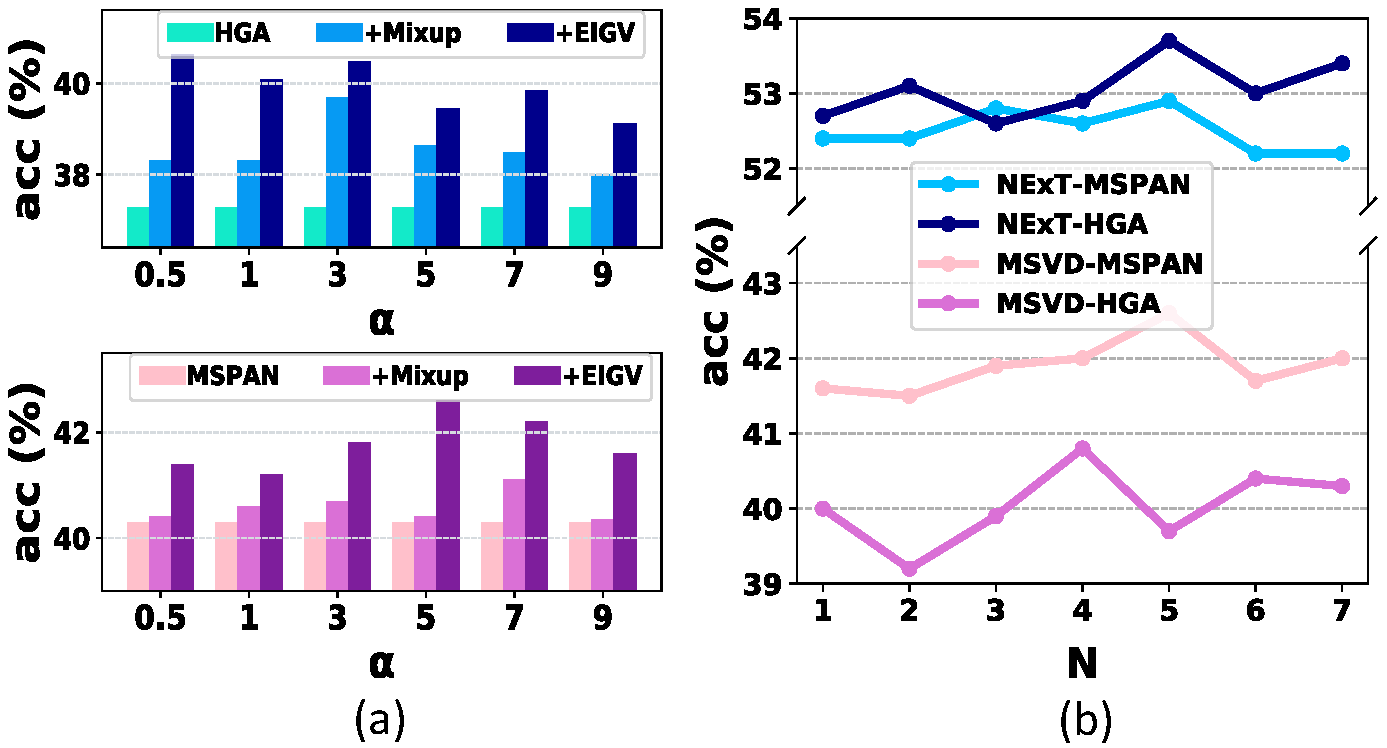
\includegraphics[scale=0.35]{fig/fig5.pdf}
\vspace{-10pt}
\caption{Hyperparameter analysis. (a) Study of $\alpha$ on MSVD-QA, which controls the equivariant mixing ratio by $\lambda_0\sim\text{Beta}(\alpha,\alpha)$. Performance of two EIGV enhanced models --- HGA (top) and MSPAN (bottom) are reported, alongside the SoTA backbone and mixup augmented performances.  
(b) Study on the impact of the negative sample number N, where EIGV with two backbones (\ie MSPAN and HGA) on two benchmark datasets (NExT-QA and MSVD-QA) are reported.}
\vspace{-10pt}
\label{fig:neg}
\end{figure}
\documentclass[10pt,twocolumn,letterpaper]{article}
\usepackage[rebuttal]{cvpr}

% Include other packages here, before hyperref.
\usepackage{graphicx}
\usepackage{amsmath}
\usepackage{amssymb}
\usepackage{booktabs}
\usepackage{multirow}
\usepackage[dvipsnames]{xcolor}

% If you comment hyperref and then uncomment it, you should delete
% egpaper.aux before re-running latex.  (Or just hit 'q' on the first latex
% run, let it finish, and you should be clear).
\usepackage[pagebackref,breaklinks,colorlinks,bookmarks=false]{hyperref}

% Support for easy cross-referencing
\usepackage[capitalize]{cleveref}
\crefname{section}{Sec.}{Secs.}
\Crefname{section}{Section}{Sections}
\Crefname{table}{Table}{Tables}
\crefname{table}{Tab.}{Tabs.}


\newcommand{\wx}[1]{{\color{green}{#1}}}
\newcommand{\blue}[1]{{\color{blue}{#1}}}
\newcommand{\pink}[1]{{\color{magenta}{#1}}}
% If you wish to avoid re-using figure, table, and equation numbers from
% the main paper, please uncomment the following and change the numbers
% appropriately.
%\setcounter{figure}{2}
% \setcounter{table}{4}
%\setcounter{equation}{2}

% If you wish to avoid re-using reference numbers from the main paper,
% please uncomment the following and change the counter for `enumiv' to
% the number of references you have in the main paper (here, 6).
%\let\oldthebibliography=\thebibliography
%\let\oldendthebibliography=\endthebibliography
%\renewenvironment{thebibliography}[1]{%
%     \oldthebibliography{#1}%
%     \setcounter{enumiv}{6}%
%}{\oldendthebibliography}


%%%%%%%%% PAPER ID  - PLEASE UPDATE
\def\cvprPaperID{7878} % *** Enter the CVPR Paper ID here
\def\confName{CVPR}
\def\confYear{2022}

%THIS PREAMBLE CONTAINS A LIST OF COMMANDS THAT ARE USEFUL FOR, AND CAN BE INCLUDED IN, EACH CHAPTER!

\usepackage{multicol}        % used for the two-column index
\usepackage[bottom]{footmisc}% places footnotes at page bottom
\usepackage{enumitem}

\usepackage{newtxtext}       % 

%REMOVED NEXT LINE SINCE IT IS NOT WORKING FOR A. SEREBRENIK AND IT DOES NOT SEEM TO BE NEEDED:
%\usepackage[varvw]{newtxmath}       % selects Times Roman as basic font

\usepackage{url}
\usepackage{pifont}

\usepackage{algorithm}% http://ctan.org/pkg/algorithms
\usepackage{algpseudocode}% http://ctan.org/pkg/algorithmicx
\usepackage{booktabs}
%\usepackage[tight,footnotesize]{subfigure} %TOM: COMMENTED OUT SINCE CONFLICTING WITH subcaption PACKAGE!
\usepackage{multirow}
\usepackage{wrapfig}
\usepackage{listings}
\usepackage{siunitx}
\usepackage{pgfplotstable}
\usepackage{array}
\usepackage{subcaption}
\usepackage{newfloat}

\usepackage{pdflscape}
\usepackage{xspace}

\usepackage{diagbox} % useful for creating top left cell with explanations of tables heading 

%Semantic labeling of chapters:
%Systematically use \label{XYZ:…} for all labels used in your chapter, where XYZ is the letter code assigned to your chapter. The unique letter codes are:
%INT (for the INTtroduction to software ecosystems chapter by Mens and De Roover)
%PPM (for the Promises and Perils of Mining software ecosystem data by Kula, Inoue, Treude)
%SLU (for the Software Library Usage pattern mining chapter by Tien Nguyen)
%EMO (for the Emotion Analyses chapter by Novieli and Serebreni)
%SWH (for the SoftWare Heritage chapter by Di Cosmo and Zacchiroli)
%FRK (for the variant FoRK analysis chapter by Businge and Demeyer)
%COL (for the COLlateral evolution chapter by Lo, Bowen, Yang)
%WFA (for the WorkFlow Automation chapter by Wessel, Mens, …)
%IAC (for the Infrastructure as Code chapter by De Roover, Zeraouli, Opdebeeck)
%MDE (for the Model-Driven Engineering chapter by Di Ruscio, Nguyen, Pierantonio)
%DIS (for the Data-Intensive Software ecosystem chapter by Cleve et al)

%Refere to chapters, sections, figures, tables in a chapter using the following commands using the chapter's letter code:
\newcommand{\chap}[1]{Chapter~\ref{#1:ch}}
\newcommand{\sect}[2]{Section~\ref{#1:sec:#2}}
\newcommand{\subsect}[2]{Subsection~\ref{#1:subsec:#2}}
\newcommand{\fig}[2]{Figure~\ref{#1:fig:#2}}
\newcommand{\tab}[2]{Table~\ref{#1:tab:#2}}
\newcommand{\lst}[2]{Listing~\ref{#1:lst:#2}}

%Example for the Introduction chapter: \chap{INT}, \sect{INT}{definition}, \fig{INT}{figlabel}, \tab{INT}{tablabel}



\usepackage[]{todonotes}
\newcommand{\tom}[1]{\todo[color=yellow!40, inline]{\footnotesize{Tom: #1}}}
\newcommand{\coen}[1]{\todo[color=blue!40, inline]{\footnotesize{Coen: #1}}}
\newcommand{\anthony}[1]{\todo[color=orange!40, inline]{\footnotesize{Anthony: #1}}}

\newcommand{\alexander}[1]{\todo[color=yellow!40, inline]{\footnotesize{Alexander: #1}}}
\newcommand{\nicole}[1]{\todo[color=blue!40, inline]{\footnotesize{Nicole: #1}}}

\newcommand{\raula}[1]{\todo[color=yellow!40, inline]{\footnotesize{Raula: #1}}}
\newcommand{\katsuro}[1]{\todo[color=blue!40, inline]{\footnotesize{Katsuro: #1}}}
\newcommand{\christoph}[1]{\todo[color=blue!40, inline]{\footnotesize{Christoph: #1}}}

\newcommand{\roberto}[1]{\todo[color=yellow!40, inline]{\footnotesize{Roberto: #1}}}
\newcommand{\stefano}[1]{\todo[color=blue!40, inline, inlinewidth=2cm]{\footnotesize{Stefano: #1}}}

\newcommand{\serge}[1]{\todo[color=yellow!40, inline]{\footnotesize{Serge: #1}}}
\newcommand{\john}[1]{\todo[color=blue!40, inline]{\footnotesize{John: #1}}}

\newcommand{\mairieli}[1]{\todo[color=pink!40, inline]{\footnotesize{Mairieli: #1}}}
\newcommand{\pooya}[1]{\todo[color=orange!40, inline]{\footnotesize{Pooya: #1}}}

\newcommand{\tien}[1]{\todo[color=yellow!40, inline]{\footnotesize{Tien: #1}}}

\newcommand{\david}[1]{\todo[color=yellow!40, inline]{\footnotesize{David: #1}}}
\newcommand{\xu}[1]{\todo[color=blue!40, inline]{\footnotesize{Xu: #1}}}
\newcommand{\zhou}[1]{\todo[color=orange!40, inline]{\footnotesize{Zhou: #1}}}

\newcommand{\davide}[1]{\todo[color=yellow!40, inline]{\footnotesize{Davide: #1}}}
\newcommand{\phuong}[1]{\todo[color=blue!40, inline]{\footnotesize{Phuong: #1}}}
\newcommand{\alfonso}[1]{\todo[color=orange!40, inline]{\footnotesize{Alfonso: #1}}}

\newcommand*{\ie}{i.e.,\@\xspace}
\newcommand*{\eg}{e.g.,\@\xspace}
\newcommand*{\etal}{\emph{et~al.}\@\xspace}
\newcommand{\cmark}{\ding{51}}%
\newcommand{\xmark}{\ding{55}}%
\newcommand\revised[1]{\textcolor{blue}{#1}}

%%%% SOME COMMANDS NEEDED IN DIFFERENT CHAPTERS %%%%
\newcommand{\gh}{GitHub\xspace}
\newcommand{\github}{{GitHub}\xspace}
\newcommand{\gitea}{{Gitea}\xspace}
\newcommand{\gitlab}{GitLab\xspace}
\newcommand{\bitbucket}{BitBucket\xspace}
\newcommand{\sourceforge}{{SourceForge}\xspace}
\newcommand{\git}{\textit{git}\xspace}
\newcommand{\docker}{{Docker}\xspace}
\newcommand{\dockerhub}{{Docker Hub}\xspace}
\newcommand{\ansible}{{Ansible}\xspace}
\newcommand{\stackoverflow}{{Stack Overflow}\xspace}
\newcommand{\openstack}{{OpenStack}\xspace}
\newcommand{\npm}{{npm}\xspace}
\newcommand{\gha}{GitHub Actions\xspace}
\newcommand{\actions}{GitHub Actions\xspace}

\newtheorem{Definition}{Definition}
\newtheorem{Algorithm}{Algorithm}
\newtheorem{Claim}{Claim}
\newtheorem{Lemma}{Lemma}
\newtheorem{Theorem}{Theorem}

%%%% SOME COMMANDS NEEDED IN DIFFERENT CHAPTERS %%%%

%FOR LIBRARIES CHAPTER:
\newcommand{\code}[1]{{\footnotesize\texttt{#1}}}
\newcommand{\model}{\textsc{Groum}\xspace}
\newcommand{\miner}{\textsc{GrouMiner}\xspace}
\newcommand{\patt}{\textsc{PattExplorer}\xspace}

%%%%%%%%%%% NEEDED FOR GITHUB AUTOMATION CHAPTER %%%%%%%%%%%%%%%%%
%%%%%%%%%%% for listings of yaml code %%%%%%%%%%%%%%%%%
\newcommand\YAMLcolonstyle{\color{red}\mdseries}
\newcommand\YAMLkeystyle{\color{black}\bfseries}
\newcommand\YAMLvaluestyle{\color{blue}\mdseries}

\makeatletter

\newcommand\language@yaml{yaml}

\expandafter\expandafter\expandafter\lstdefinelanguage
\expandafter{\language@yaml}
{
  keywords={true,false,null,y,n},
  keywordstyle=\color{darkgray}\bfseries,
  basicstyle=\YAMLkeystyle,                                 % assuming a key comes first
  sensitive=false,
  comment=[l]{\#},
  morecomment=[s]{/*}{*/},
  commentstyle=\color{purple}\ttfamily,
  stringstyle=\YAMLvaluestyle\ttfamily,
  moredelim=[l][\color{orange}]{\&},
  moredelim=[l][\color{magenta}]{*},
  moredelim=**[il][\YAMLcolonstyle{:}\YAMLvaluestyle]{:},   % switch to value style at :
  morestring=[b]',
  morestring=[b]",
  literate =    {---}{{\ProcessThreeDashes}}3
                {>}{{\textcolor{red}\textgreater}}1     
                {|}{{\textcolor{red}\textbar}}1 
                {\ -\ }{{\mdseries\ -\ }}3,
}

% switch to key style at EOL
\lst@AddToHook{EveryLine}{\ifx\lst@language\language@yaml\YAMLkeystyle\fi}
\makeatother

\newcommand\ProcessThreeDashes{\llap{\color{cyan}\mdseries-{-}-}}
%%%%%%%%%%% End of code for listings of yaml code %%%%%%%%%%%%%%%%%

%%%%%%%%%% NEEDED FOR PROMISES AND PERILS CHAPTER %%%%%%%%%%%%%%%%%
\usepackage{wasysym}
\newcommand{\use}{Use}
\newcommand{\useBy}{UsedBy}
%%%%%%%%%% END OF CODE NEEDED FOR PROMISES AND PERILS CHAPTER %%%%%%%%%%%%%%%%%


%%%%%%%%%%% NEEDED FOR IAC CHAPTER %%%%%%%%%%%%%%%%%
\DeclareFloatingEnvironment[
    fileext=los,
    listname={List of Listings},
    name=Listing,
    placement=!h,
    within=none,
]{listing}

\lstset{
  basicstyle=\footnotesize\ttfamily,
  breaklines=true,
  breakatwhitespace=true,
  commentstyle=\color{purple}, % comment color
  keywordstyle=\color{blue}, % keyword color
  stringstyle=\color{black},
  escapeinside={<@}{@>},
  xleftmargin=1em,
  language=bash,
  numbersep=8pt,
  breakindent=1em,
  postbreak=\postbreak,
  numbers=left,
  numberstyle=\tiny\ttfamily,
}

\lstdefinestyle{docker}{
  language=bash,
  morekeywords={RUN,FROM,MAINTAINER},
  showstringspaces=false,
  frame=none,
}
\lstdefinelanguage{ansible}{
  morekeywords={name,vars,hosts,tasks,roles,role},
  keywordstyle=\bfseries,
  morecomment=[l][\textit]\#,
  morecomment=[s][\bfseries]{\{\{}{\}\}},
}
\lstdefinestyle{ansible}{
  language=ansible,
  basicstyle=\scriptsize\ttfamily,
}

\def\postbreak{%
  \raisebox{0ex}[0ex][0ex]{\ensuremath{\hookrightarrow\space}}}
%%%%%%%%%%% END OF CODE NEEDED FOR IAC CHAPTER %%%%%%%%%%%%%%%%%

%%%%%%%%%%% NEEDED FOR MDE CHAPTER %%%%%%%%%%%%%%%%%
\lstdefinestyle{searchstringstyle}{
	basicstyle=\ttfamily\footnotesize,
	breakatwhitespace=false,         
	breaklines=true,                 
	captionpos=t,                    
	keepspaces=true,                 
	numbers=none,                    
	numbersep=5pt,                  
	showspaces=false,                
	showstringspaces=false,
	showtabs=false,                  
	tabsize=2,
	frame=single
}
%%%%%%%%%%% END OF CODE  FOR MDE CHAPTER %%%%%%%%%%%%%%%%%

%%%%%%%%%%% NEEDED FOR LIBRARIES CHAPTER %%%%%%%%%%%%%%%%%
\definecolor{mauve}{rgb}{0.58,0,0.82}
\definecolor{dkgreen}{rgb}{0,0.6,0}
\definecolor{gray}{rgb}{0.5,0.5,0.5}

\lstset{frame=tb,
  language=Java,
  aboveskip=3mm,
  belowskip=3mm,
  showstringspaces=false,
  columns=flexible,
  basicstyle={\small\ttfamily},
  numbers=left,
  numberstyle=\tiny\color{gray},
  keywordstyle=\color{blue},
  commentstyle=\color{dkgreen},
  stringstyle=\color{mauve},
  breaklines=true,
  breakatwhitespace=true,
  tabsize=4
}
%%%%%%%%%%% END OF CODE  FOR LIBRARIES CHAPTER %%%%%%%%%%%%%%%%%



% \newcommand{\Brittany}[1]{[\textbf{Brittany}:~{\color{purple} #1}]}
\newcommand{\Markus}[1]{[\textbf{Markus}:{\color{magenta} #1}]}
\newcommand{\Christoph}[1]{[\textbf{Christoph}:~{\color{blue} #1}]}

\newcommand{\ts}{TypeScript}
\newcommand{\js}{JavaScript}

%research questions
\newcommand{\rqone}{What errors does \ts\ detect in NPM documentation?}
\newcommand{\rqtwo}{How does error detection differ between ESLint and \ts?}
\newcommand{\rqthree}{What is the impact of NCC on the set of NPM snippets?}
\newcommand{\rqfour}{How does NCC compare to NCQ's code corrections?}
\newcommand{\rqfive}{How does NCC compare to manual fixes?}

%hyperref setup
\hypersetup{
    colorlinks=true,
    linkcolor=blue,
    anchorcolor=blue,
    filecolor=blue,      
    citecolor=blue,
    urlcolor=blue
}

%define colours
\definecolor{lightgreen}{rgb}{0.8,1,0.8}
\definecolor{lightyellow}{rgb}{1,1,0.8}
\definecolor{lightred}{rgb}{1,0.8,0.8}
\definecolor{baseColour}{RGB}{255, 128, 85}
\definecolor{ncqColour}{RGB}{118, 165, 175}
\definecolor{ncqColour2}{RGB}{162, 196, 201}

%algorithm comment style
\newcommand\mycommfont[1]{\footnotesize\ttfamily\textcolor{blue}{#1}}
\SetCommentSty{mycommfont}
%alg options
\SetAlFnt{\small}
\SetAlCapFnt{\small}
\SetAlCapNameFnt{\small}
\algsetup{linenosize=\tiny}

%lsting setup
\lstdefinelanguage{javascript}{
    keywords={typeof, new, true, false, catch, function, return, null, catch, switch, var, if, in, while, do, else, case, break},
    keywordstyle=\bfseries,
    ndkeywords={class, export, boolean, throw, implements, import, this},
    ndkeywordstyle=\color{darkgray}\bfseries,
    identifierstyle=\color{black},
    sensitive=false,
    comment=[l]{//},
    morecomment=[s]{/*}{*/},
    commentstyle=\color{blue}\ttfamily,
    stringstyle=\color{purple}\ttfamily,
    morestring=[b]',
    morestring=[b]"
}
\newcommand{\lstbg}[3][0pt]{{\fboxsep#1\colorbox{#2}{\strut #3}}}
\lstdefinelanguage{diff}{
    morecomment=[f][\lstbg{lightgreen}]+,
    morecomment=[f][\lstbg{lightred}]-,
    morecomment=[f][\lstbg{lightyellow}]\\,
    keywords={typeof, new, true, false, catch, function, return, null, catch, switch, var, if, in, while, do, else, case, break},
    keywordstyle=\bfseries,
    ndkeywords={class, export, boolean, throw, implements, import, this},
    ndkeywordstyle=\color{darkgray}\bfseries,
    identifierstyle=\color{black},
    sensitive=false,
    morecomment=[s]{/*}{*/},
    commentstyle=\color{blue}\ttfamily,
    stringstyle=\color{purple}\ttfamily,
    morestring=[b]',
    morestring=[b]"
}
\lstset{
    frame = single,
    tabsize=1,
    showstringspaces=false,
    language=javascript,
    basicstyle=\fontsize{7}{6}\selectfont\ttfamily,
    breaklines=true, 
    breakatwhitespace=false,   % sets if automatic breaks should only happen at
    numbers=left, 
    firstnumber=1,
    numberstyle=\tiny, 
    stepnumber=1, 
    numbersep=5pt,
    float,
    aboveskip=0pt,
    belowskip=0pt,
    xleftmargin=.02\textwidth,
    xrightmargin=.02\textwidth,
    escapeinside={\%*}{*)},          % if you want to add LaTeX within  % your code 
}

\addto\extrasenglish{%
  \def\chapterautorefname{Chapter}%
  \def\sectionautorefname{Section}%
  \def\algorithmautorefname{Algorithm}%
  \def\subsectionautorefname{Section}%
  \def\subsubsectionautorefname{Section}%
}

%tikz
\usetikzlibrary{
    arrows.meta,
    chains,
    scopes,
    positioning,
    shapes.geometric
}
% layers
\pgfdeclarelayer{background}
\pgfdeclarelayer{foreground}
\pgfsetlayers{background,main,foreground}

% styles     
\tikzset{
    processDiagram/.style={
        startstop/.style={
            rectangle,
            draw,
            minimum width=3cm, 
            minimum height=0.8cm,
            join = by arrow,
            fill = black!0,
        },
        decision/.style = {
            diamond,
            aspect=1.7,
            draw,
            minimum width=2.5cm, 
            minimum height=1cm, 
            align=center,
            join = by arrow,
            fill = black!0,
        },
        process/.style = {
            rectangle, 
            rounded corners, 
            draw,
            minimum width=3cm,
            minimum height=0.8cm, 
            align=center,
            join = by arrow,
            fill = black!0,
        },
        process2/.style = {
            rectangle, 
            rounded corners, 
            draw,
            minimum width=3cm,
            minimum height=0.8cm, 
            align=center,
            join = by arrow,
            fill = ncqColour2,
        },
        line/.style = {
            -
        },
        invisible/.style = {
            join = by line,
            minimum width=0cm, 
            minimum height=0cm,
            inner sep=0pt,
        },
        invisititle/.style ={
            font = \bfseries,
            join = by arrow,
            outer sep = 5pt,
        },
        title/.style = {
            font = \bfseries,
            fill = black!20,
            join = by arrow,
            minimum width = 3cm,
            minimum height=0.8cm,
            draw,
        },
        output/.style ={
            join = by line,
            minimum width=0cm, 
            minimum height=0cm,
            inner sep=0pt,
            font = \itshape,
            align = center,
        },
        arrow/.style = {
            ->
        },
    }
}


\begin{document}

%%%%%%%%% TITLE - PLEASE UPDATE
\title{Invariant Grounding for Video Question Answering}  % **** Enter the paper title here

\maketitle
\thispagestyle{empty}
\appendix

%%%%%%%%% BODY TEXT - ENTER YOUR RESPONSE BELOW

We gratefully thank all the reviewers for their valuable and constructive comments. We are encouraged that they find our topic interesting and important (R2, R3, R4, R6), our idea novel and insightful (R2, R3, R4, R6), our method effective (R2, R3, R4), and our representation clear and enjoyable-to-read (R1, R4). We receive a \emph{strong accept}, two \emph{weak accept}, and a \emph{weak reject}. We will carefully revise our paper by taking into account all the suggestions. Please find the point-to-point responses as follows.

% Thank all reviewers for their efforts and \wx{insightful comments}. We are glad that all reviewers acknowledge our novelty and motivation. We receive a \textit{strong accept}, two \textit{weak accept}, and a \textit{weak reject}.


% We thank the review from R4, but R4 mainly focuses on the expression within a single sentence or table, rather than the gist of our principle. Since we are  revisiting VideoQA from a brand-new angle, one may find these delicate causal concepts cumbersome, while others like R2 enjoy reading. We apologize for the roughness and appreciate R4's efforts. However, according to the CVPR reviewer's guideline, ``we recommend you embrace the novel, brave concept'', and the presentation details should not be the reason for rejection. Nevertheless, we will polish the language toward general satisfaction. 


\vspace{2pt}
\noindent
$\triangleright$\pink{Reviewer \#2.} \blue{Q1: The sampling strategy of complement stratification (\cf Line 457).}
A1: Thanks. For simplicity, we randomly sample the complement stratification from a memory bank to pair the grounded causal scene, to perform the causal interventions.
\blue{Q2: Visualization of causal and complement scenes predicted by Equation (9).}
A2: Thanks for the suggestions. In Figure 5 of our paper, we have showcased the visualizations, where the causal scenes are highlighted and the rests are the complement scenes. Furthermore, we have offered analyses in Section 5.3, which validate the explainability of our IGV method.


\vspace{2pt}
\noindent
$\triangleright$\pink{Reviewer \#3.}
\blue{Q1: Optimization of the scene intervener module.}
Thanks. Actually, the scene intervener module is non-parametric, \ie no model parameters are needed to optimize. It is the combination of two components: (1) a complement collector, which collects the complement estimations of videos appearing in the previous batch, and (2) a complement stratification sampler, which randomly yields complement stratification to intervene the videos in the current batch.
With the improvements of causal grounding, this module will be updated with high-quality complements.
We will clarify this point in the final paper.
\blue{Q2: Effect of the causal grounding result on the performance.}
Great catch! The modules of causal grounding and scene intervener aim for the shared goal of distinguishing the causal scenes from the complement scenes, thus playing the cooperative game and mutually improving each other.
That is, with the improvements of causal grounding, the scene intervener module will capture high-quality complements; in turn, under the guidance of the scene intervener, the causal grounding module will shape the grounding.
% In the final paper, we will showcase the progressive improvements of these two modules via qualitative and quantitative studies.

\vspace{2pt}
\noindent
$\triangleright$\pink{Reviewer \#4.}
\blue{Q1: Relation \& Difference between causal look and statistical learning.}
Great catch! In general, causal inference and statistical inference are distinct \cite{pearl2009causal}.
At the core of statistical inference (\eg regression, estimation, hypothesis test) is to assess the distribution from samples. As long as the distribution remains the same, statistical learning techniques (\eg CNN) perform well.
Causal inference goes one step further: its goal is to infer not only probabilities under static conditions, but also the causal relationship under changing conditions (\eg intervention, counterfactual).
Specifically, statistical analysis cannot measure one property of distribution that ought to vary when another property is modified. In contrast, causality identifies relationships that remain invariant when conditions change (\eg generalization ability).
Meanwhile, causal inference and statistical inference are also highly connected --- solving causal problems requires the standard statistical language with a paradigmatic shift.
\blue{Q2: Relation \& Difference between intervened and adversarial scenes.}
Good point! The scene intervention can be viewed as causality-guided data augmentation, where the intervened complements can result from either causal intervention or adversarial learning.
Here we embraced the former so that the framework can be trained in a simple, end-to-end, and effective fashion.
\blue{Performance on TGIF-QA.}
Thanks. We present the performance on TGIF-QA as follows:
\vspace{-10pt}
\input{tab/tgif-rebuttal}

\vspace{9pt}
\noindent
$\triangleright$\pink{Reviewer \#6.}
\blue{Q1: Typos.}
A1: Thanks for bringing them to us. We sincerely appreciate and promise to revise thoroughly.
\blue{Q2: Frame- \& Region-level Grounding.}
A2: Thanks. In Section 7 of our paper (\cf Line 858), we have stated the frame-level grounding's limitations and listed the region-level grounding as our future work.
Here are more clarifications: our current work aims to present and verify a novel training paradigm for VideoQA in general, instead of the effect of feature granularity; moreover, as most of the SOTA VideoQA models adopt the frame-level reasoning, our IGV stays with this tendency for adaptability and consistency.
\blue{Q3: Shared video encoder with grounding indicator.}
A3: Thanks. To reduce the computation cost, we use the shared video encoder in the grounding indicator. Difference encoders might be more effective, which is for our future exploration.
\blue{Q4: Baseline method in Table 4.}
A4: Sorry for the confusion. The baseline indicates the backbone SOTAs without our IGV strategy. We update Table 4 as: 
\vspace{-15pt}
% \input{tab/ablation-loss-rebuttal} 
\begin{table}[ht]
\small
  \centering
  \caption{Study of IGV loss components}
   \vspace{-10pt}
    \resizebox{0.99\linewidth}{!}{
    \begin{tabular}{l|cc|cc}
    \toprule
    \multirow{2}[1]{*}{Variants} & \multicolumn{2}{c}{MSVD-QA} & \multicolumn{2}{c}{MSRVTT-QA} \\
          & Our Backbone   & Co-Mem & Our Backbone   & Co-Mem \\
    \midrule
    \midrule
    Baseline & 36.1  & 34.6  & 36.3  & 35.3 \\
    $\Lapl_{\hat{c}}$     & 36.0    & 33.3  & 36.7  & 36.0 \\
    $\Lapl_{\hat{c}}+\Lapl_{\hat{t}}$   & 37.4  & 36.1  & 37.8  & 36.8 \\
    $\Lapl_{\hat{c}}+\Lapl_{v^{*}}$   & 38.2  & 36.3  & 37.4  & 36.2 \\
    $\Lapl_{\hat{c}}+\Lapl_{\hat{t}}+\Lapl_{v^{*}}$ & \textbf{40.8} & \textbf{37.7} & \textbf{38.3} & \textbf{37.3} \\
    \bottomrule
    \end{tabular}
    }
  \label{tab:ablation-loss}%
  \vspace{-15pt}
\end{table}%

% \vspace{2pt}
% \noindent
% $\triangleright$\pink{Reviewer \#2.} \blue{Q1. The sampling strategy in Line 457 is not explained. Is it randomly sampled?}
% A1: Thanks. Yes, the complement stratification is randomly sampled. 
% \blue{Q2. Visualizing or statistically analyzing the causal and complement scenes predicted by Formula 9 could strengthen the explainability of this method.}
% A2: Good suggestion, we have exactly such visualization in Figure 5, where the highlighted part is the causal scene and the rest is the complement scene.


% \vspace{2pt}
% \noindent
% $\triangleright$\pink{Reviewer \#3.} \blue{Q. As the scene intervener relies on the causal grounding result. I wonder how to optimize this module? Would the causal grounding result affect the performance? If the causal grounding module is not well-trained, the scene intervener might not synthesize reliable videos. I imagine the training of the model is not very straightforward.}
% A: Good question. The grounding result is fundamental to our framework. To achieve that, we carefully designed our training objective with two auxiliary loss Eq 12-13 that enables the grounding indicator trained in an end-to-end fashion.  

% \vspace{2pt}
% \noindent
% $\triangleright$\pink{Reviewer \#4.} \blue{Q1. Is causal look another statistical learning?
% This paper argues that ERM blindly captures all statistical relations. To deal with this problem, they adopt a causal look, which analyzes data from a causal point of view. Thus, the proposed method also belongs to statistical learning. Please explain the difference between them.}

% \blue{Q2. Whether Complement Scene is a technical enhancement? I think the operation of changing the complement scene is similar to adversarial learning since “intervened videos” is a lot like a generated adversarial example.}
% A: Good point, the 'intervened videos' can be derived via either causal intervention or adversarial training, we embraced the former so that the framework can be trained in an end-to-end fashion.

% \blue{Q. How about the performance in TGIF-QA dataset?
% TGIF-QA dataset also is a large-scale videoqa, which is widely adopted in existing work and has more challenging. Please report the performance in TGIF-QA dataset}
% A: We have followed your suggestions to conduct experiments on three subtasks of TGIF-QA, here is the result:
% \input{tab/tgif-rebuttal}
% we didn't include TGIF-QA initially, because 1) recent analysis \cite{DBLP:conf/mm/PengYBW21} shows the severe answer biases in TGIF-QA (the "distractor" is not distracting enough, 90\% accuracy can be achieved by only using the candidate answers). 2) the video is trimmed to a very short length, which is not practical in real-world scenarios.

% \vspace{2pt}
% \noindent
% $\triangleright$\pink{Reviewer \#6.} \blue{The paper writing is poor and hard to read. It contains many grammatical errors,
% e.g. We then analyze ERM's suffering from the spurious correlations.But only part of the scenes are critical to answering the question of interest, while the rest hardly offers information relevant to the question.
% A in-depth comprehension.}
% A: Thanks for the careful review, we apologize for the roughness. We will do grammar checks thoroughly and  polish the language.

% \blue{Though well-motivated, the framework is not well-designed. The model is better to attend to related regions in related video frames. However, the proposed method only attends to related video frames without region-level attention in video frames.}
% Thanks, (this agrees with our discussion/ as discussed) in Section 7 (L858), we do anticipate fine-grained region-level features will strengthen the current IGV design, and this will be part of the future work. However, in this work, we aim to present and verify a novel training paradigm for VideoQA in general, instead of the effect of feature granularity. On the other hand, most of the VideoQA SoTAs adopt frame-level reasoning, so IGV stays with this tendency for adaptability and consistency.

% \blue{Why the video encoder is shared with the grounding indicator?}
% To save computation cost, it's not imperative.
% \blue{What is the baseline method in Table 4?}
% Sorry for the confusion, the baseline indicates backbone SoTAs without enhancement from invariant grounding strategy (identical to Table 3), where the IGV indicates Our Backbone. We revise Table 4 as below for your reference. 
% \input{tab/ablation-loss-rebuttal} 





%%%%%%%%% REFERENCES
{\small
\bibliographystyle{ieee_fullname}
\bibliography{macros,main}
}

\end{document}

\section{Preliminaries}
\label{sec:preliminaries}

Here we provide a holistic view of VideoQA by summarizing a common paradigm throughout existing works. Specifically, we denote a variable and its deterministic value by upper-cased (\eg $A$) and lower-cased (\eg $a$) letters, respectively. 

\vspace{5pt}
\noindent\textbf{Modeling}.
Given the video $V$, the VideoQA model $f_{\hat{A}}{(\cdot)}$ answers the question $Q$ by formulating the visual-linguistic alignment: 
\begin{gather}\label{eq:conventional-modeling}\
    \hat{A} = f_{\hat{A}}(V,Q),
\end{gather}
where $\hat{A}$ is the predictive answer. Typically, $f_{\hat{A}}{(\cdot)}$ is a combination of two modules: 
\begin{itemize}[leftmargin=*]
    \item Video-question encoder, which warps up the visual content and linguistic semantics via two encoders: (1) the video encoder capsules the video content by methods like hierarchical design \cite{DBLP:conf/mm/PengYBW21, dang2021hierarchical, le2021hierarchical}, enhanced memory architecture \cite{gao2018motionappearance, fan2019heterogeneous} and structural graph representation  \cite{jiang2020reasoning,huang2020locationaware,DBLP:conf/acl/GuoZJ0L20, Wang_2018_ECCV}; (2) the question encoder embeds the contextual information into linguistic representation through multi-scale semantic integration \cite{jiang2020reasoning, DBLP:conf/acl/SeoKPZ20, 2021} or grammatical dependencies parsing \cite{park2021bridge}.
    
    \item Answer decoder, which abridges the encoded visual-linguistic information via cross-modal interaction methods like graph alignment \cite{ park2021bridge} and progressive attention \cite{DBLP:conf/acl/SeoKPZ20, DBLP:conf/mm/PengYBW21}, then generates the prediction accordingly.
    % \item Answer decoder, which abridges the visual-linguistic information to generate the prediction. Based on the encoded representation, the cross-modal interaction is learned via graph alignment \cite{ park2021bridge} or progressive attention \cite{DBLP:conf/acl/SeoKPZ20, DBLP:conf/mm/PengYBW21}.
\end{itemize}

\vspace{5pt}
\noindent\textbf{Learning}.
\wx{To optimize the video-question encoder and answer decoder, current VideoQA models usually adopt the scheme of empirical risk minimization (ERM) \cite{gao2018motionappearance,le2021hierarchical,jiang2020reasoning,DBLP:conf/mm/PengYBW21}, which measures and minimizes the risk between the ground-truth answer $A$ and predictive answer $\hat{A}$:}
\begin{gather}\label{equ:erm-loss}
    \min\mathcal{L}_{\text{ERM}}(\hat{A}, A).
\end{gather}
In essence, ERM recklessly takes the video content as a whole and enforces the risk deduction over compassion of question and every video frame, which \wx{hardly discovers a reliable interpretation to exhibit the visual-linguistic alignment}.

% In essence, ERM encourages these VideoQA modules to capture the statistical correlations between answer and video content as a whol

% where $\mathcal{L}_{\text{ERM}}$ is the risk function that measure the entropy between the predictive answer $\hat{A}$ and ground-truth answer $A$, which is usually set as cross-entropy loss  \cite{gao2018motionappearance,le2021hierarchical} or hinge loss \cite{fan2019heterogeneous,jiang2020reasoning,DBLP:conf/cvpr/XiaoSYC21}.
% % ERM is consistent with the criterion of mutual information maximization, which maximizes the mutual information between .
% In essence, ERM encourages these VideoQA modules to capture the statistical correlations between the video-question pairs and answers.






\section{Introduction}
\label{sec:introduction}


% 1.videoQA overview-----------------------------------------
Video Question Answering (VideoQA) \cite{fan2019heterogeneous} is a keystone in interactive AI, such as vision-language navigation and communication systems.
It aims to answer the natural language question based on the video content.
Striving for the architecture novelty, many studies have been conducted on modeling VideoQA's multi-modal nature, such as fostering the vision-language alignment \cite{jiang2020reasoning,park2021bridge} and revisiting the visual input structure \cite{le2021hierarchical,dang2021hierarchical}.
However, existing VideoQA models usually operate as black boxes, which fail to exhibit the working mechanism behind the predictions and hardly exhibit ``What knowledge should the model use to answer the question about the video?''.
As a result, the black-box nature causes concern for the model's reliability, especially in applications to safety and security.



\begin{figure}[t]
\centering
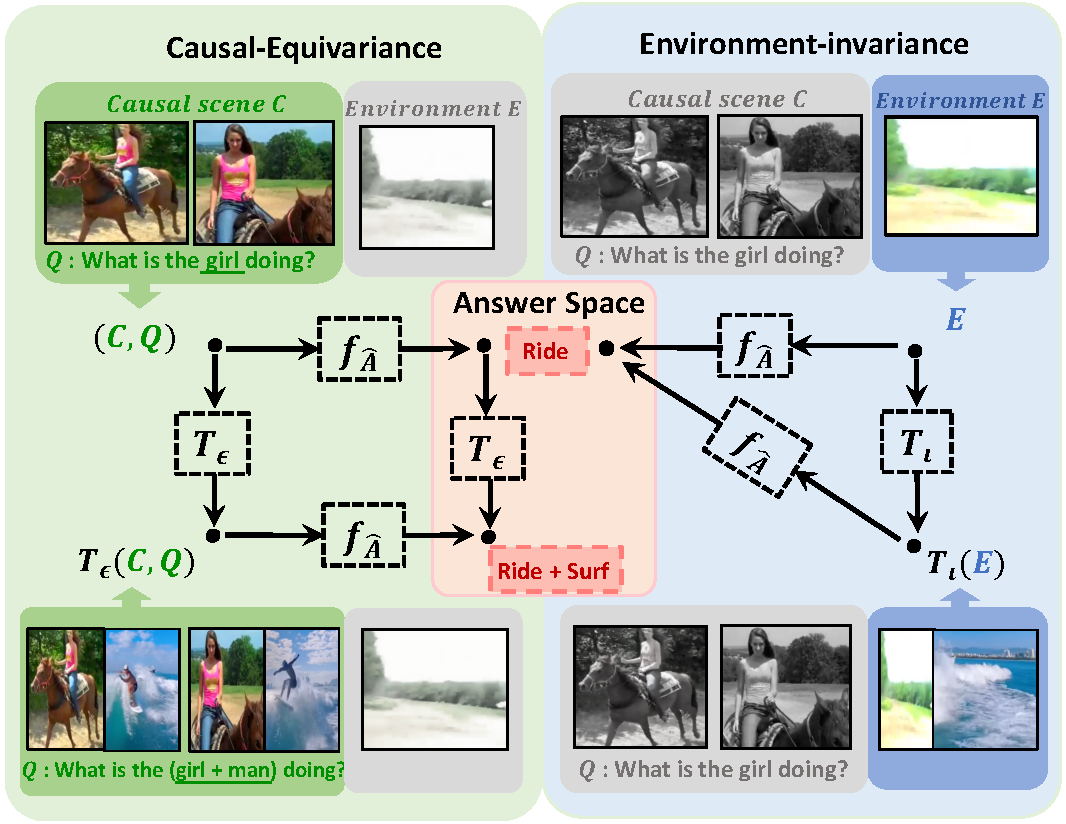
\includegraphics[scale=0.47]{fig/f1.pdf}
\vspace{-15pt}
\caption{
Illustration of equivariant and invariant grounding.
The causal-equivariant principle (left) asks that the semantic change $T_{\epsilon}$ applied to the causal scene $C$ and question $Q$ should be faithfully reflected in the answer change.
In contrast, the environment-invariant principle (right) outputs the same answer, regardless of changes $T_{\iota}$ on the environment scene $E$.
Here, $f_{\hat{A}}$ maps input to answer space.
% On the left, transformation $T_{\epsilon}$
% Illustration of causal-equivariant and environment-invariant principles.
% On the left, transformations $T_{\epsilon}$ convert the causal scene $C$ and question $Q$ into intervened factors (exemplified as a mixture with the ``man-surfing-in-ocean'' sample) which reflects equivariance in the answer space. On the right, transformation $T_{\iota}$ mixed the two environment scenes and yields an invariant answer. Here, $f_{\hat{A}}$ maps input to answer space.
}
\vspace{-15pt}
\label{fig:overview}
\end{figure}


% 2.problem of interpretable-------------------------------
The concern on the black-box nature calls for better explainability of VideoQA models.
Here we focus on visual-explainability \cite{CSS,DBLP:conf/ijcai/RossHD17}, aiming to reveal ``Which part of the video should the model look at to answer the question?''.
It requires us to find a subset of visual scenes --- rationale --- which are the right reasons for the right answering \cite{DBLP:conf/ijcai/RossHD17}.
Taking Figure \ref{fig:overview} as an example, when answering the question ``What is the girl doing?'', the rationale should focus on the ``girl-riding on-horse'' scene in the first two clips.
Towards this end, existing studies \cite{gao2018motionappearance,DBLP:conf/iccv/Liu0WL21,DBLP:conf/mm/WangG0W21} dwell mainly on the paradigm of \textbf{post-hoc explainability} \cite{LIME,DBLP:conf/iccv/SelvarajuCDVPB17}, which distributes the predictive answer of the target model to the input visual features via an additional explainer method.
They visualize the attention weights or gradient-like signals toward the visual features, and then identify a salient pattern as the rationale.
However, post-hoc explainability has several major limitations:
(1) It fails to make the target model intrinsically interpretable \cite{DBLP:conf/cvpr/YangZQ021,wang2021causal,DBLP:journals/natmi/Rudin19},  only approximating the decision-making process of the model.
As a result, the identified rationale cannot faithfully reveal how the model leverages the multi-modal information.
(2) Such visual inspections are fragile against input perturbations, since some artifacts can be easily captured as explanations instead of genuine knowledge from the data \cite{DBLP:conf/ijcai/LaugelLMRD19,slack2020fooling,heo2019fooling,ghorbani2019interpretation}.




% 3.partition the video to get interpretation ------------
The limitations of post-hoc explainability inspire us to explore the paradigm of \textbf{intrinsic interpretability} \cite{ghorbani2019interpretation,DBLP:journals/natmi/Rudin19}, which embeds a rationalization module into the model to make the decision-making process transparent.
Surprisingly, the intrinsic interpretability of VideoQA models is until-now lacking.
To fill the void, we draw on \textbf{causal theory} \cite{pearl2016causal,pearl2009causal} to formulate the interpretability task as disclosing ``Which part of the video is critical/causal to answering the question?''.
Concretely, we aim to identify the causal component of input video on-the-fly, which holds the question-response information and filters out the question-irrelevant cues.
Following this essence, one straightforward realization is to ground the input video into two segments:
(1) \textbf{causal scene}, which retains the question-critical visual content and sufficiently approaches the answer, thus naturally serving as the rationale;
and (2) \textbf{environment scene}, which holds the question-irrelevant visual content and can be seen as the rationale's complement.



% 4.euiqvariant and invariant -------------------------------
% 要突出的是grounding,title中是Equivariant and invariant grounding,所以要让这些关键词尽早的出现。
% 这个例子融入到下面的Causal-Equivariance和Environmental-Invariance中去。
%
However, discovering causal scene without the supervision of ground-truth rationale is challenging.
With a causal look at the reasoning process (\cf Section \ref{sec:causal-view}), we argue that the crux of intrinsic interpretability is to amplify the connection between the causal scene and the answer, while blocking the non-causal effect of the environment scene.
Following this line, we propose two principles to guide the grounding of the rationale:
\begin{itemize}[leftmargin=*]
    \item \textbf{Causal-Equivariance.}
    By ``equivariance'', we mean that answering should be sensitive to the semantic changes on the causal scene and question (termed E-intervention), \eg any change on the causal scene and question should be faithfully reflected on the predicted answer. For example, in Figure \ref{fig:overview}, the ``girl-riding on-horse'' and ``man-surfing in-ocean'' scenes are the oracle rationales of ``What is the girl doing?'' and ``What is the man doing?'', respectively. The intervention applied on the input (\ie mixing the ``girl-riding on-horse'' and ``man-surfing in-ocean'' scene, and combining two questions as ``What is the girl doing? What is the man doing?'') should set off an equivariant change in the answer (\ie changing from ``Ride'' to ``Ride+Surf'').
    
    
    
    \item \textbf{Environment-Invariance.}
    By ``invariance'', we mean that answering should be insensitive to the changes in the environment scene (termed I-intervention), conditioning on the causal scene and question.
    Considering Figure \ref{fig:overview} again, the intervention applied to the environment (\ie mixing the ``meadow'' and ``ocean'' scenes) implies no impact towards answering ``What is the girl doing?'', reflecting a homogeneity in the answer space.
\end{itemize}


%5.overall idea ------------------------------------------------------------------
% Aspiring to capture grounding rationale, we formalize a model-agnostic learning framework, Equivariant and Invariant Grounding for Interpretable VideoQA (EIV), 
% %
% by asking the question ``what and how transformation should the model be equivariant or invariant to?'' 
% %
% Different from the previous effort that design supervised proxy task for geometric transformation \cite{DBLP:conf/iccv/ChengSM21}, 
% % we adopted philosophy of causal intervention and design a saliency-aware temporal mix method for the video input, and impose 
% we answer the ``what'' question by adopting the philosophy of causality \cite{pearl2009causal} and configure transformation as causal intervention operation that imposes scene-aware mixup \cite{DBLP:conf/iclr/ZhangCDL18} on the multi-modal input.
% %
% As for the question of how, we present a unified view of equivariant and invariant principles via the lens of temporal self-supervised learning, where the contrastive counterparts are bred through a disruption on the causal scene, environment scene as well as vision-language alignment.

% where the contrastive counterparts are bred through a disruption on the causal and environment scene, respectively.

% implemetation ----------------------------------------------
% 这一段的写作逻辑应该是如何实现equivariant、invariant principles的;可以不用follow IGV的写法;

% 可以这么组织:
% 一句话介绍三个modules;
% 然后如何用这三个modules来实现两个principle的:首先用grouidng indicator去roughly partition videos into two parts:causal and environmental scenes;然后基于这两部分引入causal-equivariance:利用interventer对于causal scenes做interventions,期望answer部分产生相对应的变化;利用interventer对于environmental scenes做interventions,期待这部分不会对于answering产生影响。

To impose these two principles for intrinsic interpretability, we propose a new framework, \underline{E}quivariant and \underline{I}nvariant \underline{G}rounding for Interpretable \underline{V}ideoQA (\textbf{EIGV}).
EIGV equips the VideoQA backbone model with three additional modules:
a grounding indicator, an intervener, and a disruptor.
First, the grounding indicator learns to attend the causal scene based on the input question, while leaving the rest as the environment.
% However, this grounding only roughly estimates the oracle partition of causal and environment scenes.
Then, the intervener parameterizes the proposed principles to guide the grounding.
Specifically, towards the causal-equivariance principle, it conducts the E-intervention on the causal scene and question --- that is, mix them with the counterparts from another video-question pair --- and encourages the predictive answer to be anticipated accordingly.
Towards the environment-invariance principle, when leaving the causal scene and question untouched, it applies the I-intervention on the environment --- that is, mix it with the environmental stratification of a memory bank --- and enforces the predictive answer to be invariant.
Moreover, we build an unified sight of two principles via the lens of contrastive learning.
Concretely, on top of each intervened video-question pair, the disruptor constructs the positive views by disrupting the environment scene randomly, while creating the negative views by substituting the causal scene with random scenes.
Training with these two principles allows the backbone model to distinguish the causal scene from the environmental cues, and hinge on the critical visual-linguistic alignment. 


Briefly put, our contributions are: 
\begin{itemize}[leftmargin=*]
    \item We propose EIGV, a model-agnostic VideoQA framework that distills the causal visual-linguistic alignment to generate answers in a self-interpretable manner.
    
    \item We investigate the soundness of grounding rationale by posing the equivariant-invariant principle on visual grounding.
    
    \item We justify the superiority of EIGV on three popular benchmark datasets (\ie MSVD-QA \cite{DBLP:conf/mm/XuZX0Z0Z17}, MSRVTT-QA \cite{DBLP:conf/mm/XuZX0Z0Z17},  NExT-QA \cite{DBLP:conf/cvpr/XiaoSYC21}) with extensive experiments, where our design outmatches the state-of-the-art models. Moreover, our EIGV is a model-agnostic framework that can be applied to different VideoQA models. 
\end{itemize}














\section{Methodology}
\label{sec:method}

\begin{figure*}[t]
\centering
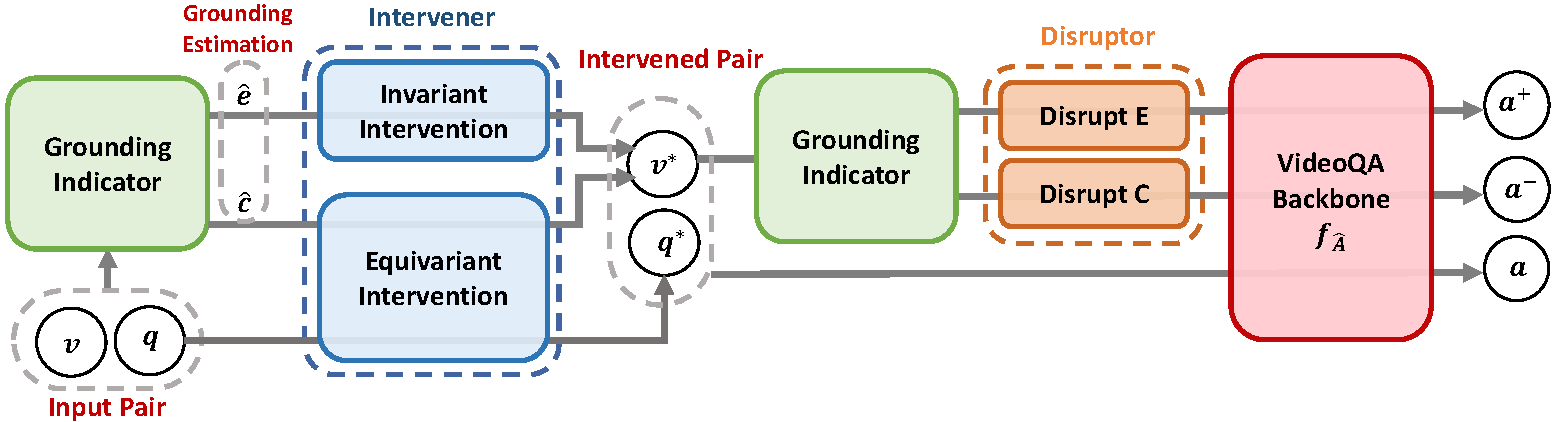
\includegraphics[width=0.95\textwidth]{fig/main.pdf}
\vspace{-14pt}
\caption{Overview of EIGV. It comprises three additional modules on top of the conventional VideoQA backbone: 1) Grounding indicator, 2) Intervener, and 3) Disrupter. First, the grounding indicator learns the estimation of causal scene $\hat{c}$ and environment $\hat{e}$. Next, two interventions are imposed on the causal and non-causal factors to compose the intervened pair $(v^*,q^*)$. Finally, based on the re-grounded result, the disruptor creates contrastive samples, which are further feed into the VideoQA backbone.}
\vspace{-5pt}
\label{fig:main}
\end{figure*}

\wx{
To ground the causal scene $C$ in the video $V$, we take a closer look at the VideoQA SCM (\ie Figure \ref{fig:scm}a), and emphasize the essential differences between $C$ and $E$.
Specifically, given the causal scene $C$ and question $Q$, the answer $A$ is determined, regardless of the variations in the environment scene $E$:}
\begin{gather}\label{equ:eq0}
      A\bot E \mid C,Q,
\end{gather}
where $\bot$ denotes the probabilistic independence. 
%

\vspace{5pt}
\noindent\textbf{Rationalization.} 
During training, the oracle grounding rationale $C$ is out of reach, while only the input $(V, Q)$ pair and training target $A$ are observed. 
Such an absence motivates VideoQA to embrace video grounding in its modeling. 
Specifically, in light of question $Q$, the estimated causal scene $\hat{C}$ is grounded from the massive $V$ to approach the oracle $C$ and then generate prediction $\hat{A}$ via $Q \rightarrow A \leftarrow C$. 
To systematize this relation, the causal-equivariance principle introduces an equivariant transformation $T_\epsilon$ to each of the parent variables (\ie $C$ and $Q$), and expects a proportionate change in the response variable (\ie $A$). On top of SCM, we formally present such notions as:
\begin{gather}
    T_\epsilon(\hat{A})=f_{\hat{A}}(T_\epsilon(\hat{C}),T_\epsilon(Q)). \label{equ:equivariance}
\end{gather}
Meanwhile, environment-invariant principle formulated Equation \eqref{equ:eq0} in the sense that imposing an invariant-transformation $T_\iota$ on the estimated environment $\hat{E}$ should not trigger variation of answer $A$: 
\begin{gather}
      \hat{A}=f_{\hat{A}}(T_\iota(\hat{E}),Q)),\label{equ:invariance}
\end{gather} 
To this end, we parameterize our learning framework, EIGV, as a combination of equivariant and invariant principles, which comprises three additional modules on top of the ERM-guided backbone: grounding indicator, intervener, and disruptor. In a nutshell, we display our EIGV framework in Figure \ref{fig:main}.


\vspace{5pt}
\noindent \textbf{Data representation.}
Following previous efforts \cite{jiang2020reasoning, DBLP:conf/acl/GuoZJ0L20}, we encode video instance $v$ as a sequence of $K$ fixed visual clips, while question instance $q$ is encoded into a similar form with a fixed length of language tokens $L$.
Then, visual and linguistic features are applied with a linear layer and an LSTM \cite{10.1162/neco.1997.9.8.1735}, respectively, to align their dimension. As a result, we acquire the output of linear layer $ \vb{v} \in \mathbb{R}^{k \times d}$ as the final video representation and the last hidden state of LSTM $\vb{q} \in \mathbb{R}^{d}$ as the holistic question representation.

% Following previous efforts [], video instance $v$ is encoded as a sequence of $K$ fixed visual clips $ \vb{v} \in \mathbb{R}^{k \times d_v}$, where $d_v$ is the visual feature dimension. Likewise, the question instance $q$ is encoded into similar form $ \vb{q} \in \mathbb{R}^{L \times d_q}$ but with a fixed length of language tokens L. Furthermore, $\vb{v}$ and $\vb{q}$ are respectively, applied with a linear layer and a LSTM [] to align their dimension, while we acquire the final hidden state of LSTM as a the holistic question representation $\vb{q} \in \mathbb{R}^{d}$.

\subsection{Grounding Indicator}
Scene partition is fundamental to the rationale discovery, whose core is to estimate the value of $C$ and $E$ via a hard split on video $V$. Given an input sample $(v,q)$, the grounding indicator aims to access the causal scene and environment scene via their estimated value $\hat{c}$ and $\hat{e}$ according to question $Q$. 
%
Concretely, we first construct two cross-modal attention modules to indicate the probability of each visual clip of being causal scene ($\vb{p}_{\hat{c}} \in\mathbb{R}^{K}$) 
and environment scene ($\vb{p}_{\hat{e}}\in\mathbb{R}^{K}$):
\begin{align}
    \vb{p}_{\hat{c}} &= \text{Softmax}(\text{FC}_{1}(\vb{v})\cdot\text{FC}_{2}(\vb{q})^\intercal),\\
    \vb{p}_{\hat{t}} &= \text{Softmax}(\text{FC}_{3}(\vb{v})\cdot\text{FC}_{4}(\vb{q})^\intercal),
\end{align}
where $\text{FC}_{1},\text{FC}_{2},\text{FC}_{3},\text{FC}_{4}$ are fully connected layers that align cross-modal representations.
%
However, gathering messages via a soft mask still makes the visual information on different clips overlap. 
As discussed in Section 3.2, guided by ERM, the conventional attention mechanism is unable to block the influence of $\hat{e}$, thus undermining the veracity of $\hat{c}$.
% As revealed by the ERM-guided method, the conventional attention is unable to block the influence of $\hat{t}$ thus undermining the veracity of $\hat{e}$. 
%
As a correction, the grounding indicator makes a discrete selection over the clip-wise attention result to generate a disjoint group of the causal scene. We leverage Gumbel-Softmax \cite{DBLP:conf/iclr/JangGP17} to manage a differentiable selection on attentive probabilities and compute the indicator vector $\vb{I}\in\mathbb{R}^{K\times 2}$ on the two attention scores  over each clip (\ie $\vb{p}_{\hat{c,i}}$, $\vb{p}_{\hat{e,i}}$, $i \in K$).  Formally, $\vb{I}$ is derived as:
\begin{gather}
    \vb{I} = \text{Gumbel-Softmax}([\vb{p}_{\hat{c}};\vb{p}_{\hat{e}}]), 
\end{gather}
where $[;]$ denote concatenation. The first and second column of $\vb{I}$ (\ie $I_{0}$ and $I_{1}$) index the attribution of $\hat{c}$ and $\hat{e}$ over k clips, respectively. 
%
To this end, we estimate $\hat{c}$ and $\hat{e}$ as follows:
\begin{gather}
    \hat{c} = I_{0}\cdot v ,\quad \hat{e} = I_{1}\cdot v, \quad \st v=\hat{c}+\hat{e} .
    % \hat{c} = \{I_{c,k}\cdot v_{k}|I_{c,k}=1\},\quad \hat{t} = \{I_{t,k}\cdot v_{k}|I_{t,k}=1\},
\end{gather}

% where binary masks $I_{0k}$ and $I_{1k}$ indicate the causal-environment attribution of the $k$-th clip.

\subsection{Intervener}
In absence of clip-level supervision, learning grounding indicators requires dedicated exploitation of the equivariance-invariance principle.
%
On this demand, we propose the intervener, which prompts the estimated rationale to the oracle by intervening $\hat{c}$ and $\hat{e}$. 
%
Figure \ref{fig:intervene} describes the functionality of $do(\cdot)$ --- the intervention operator that successively manipulated SCM over $E$ and $C$. Concretely, two intervention operations are configured to realize the equivariant and invariant transformation defined in Equations \eqref{equ:equivariance} and \eqref{equ:invariance}. 
%
% 这块儿写的不清楚。要牢记突出主线:two principle,所有的都是围绕这个实现的,只有我们反复强调这个,才能让reviewer印象深刻,然后才能从idea、implementation层面上都理解我们在干啥,并且觉得我们做的是对的。
% 这里可以分开写:

To fulfill the causal-equivariant principle, we design the E-intervention on the causal scene $\hat{c}$, which applies a linear interpolation between two data points on their causal factors --- $C$, $Q$ and $A$.  
By casting the same mixing ratio $\lambda_0\sim\text{Beta}(\alpha,\alpha)$ on all causal factors, the equivariant intervener learns to capture 
% the mainstay depicted in Figure \ref{fig:scm}c, so as to abridge 
the causal connection of $C, Q \to A$.
In particular, we attain the intervened causal scene $c^*\in \mathbb{R}^{K\times d}$, question $q^*\in \mathbb{R}^{d}$ and answer $a^*\in \mathbb{R}$ as follow:
\begin{gather}
    c^*=\lambda_0 \cdot \hat{c}+(1-\lambda_0) \cdot \hat{c}',\\
    q^*=\lambda_0 \cdot q+(1-\lambda_0) \cdot q',\\
    a^*=\lambda_0 \cdot a+(1-\lambda_0) \cdot a',
\end{gather}
where $\hat{c}'$, $q'$ and $a'$ are causal factors from a second sample.

To achieve the environment-invariant principle, we devise the I-intervention that adopts a similar mixing strategy to the environment scene $\hat{e}$. 
%
Notably, by drawing the mixing ratios $\lambda_1$ from a second distribution that is distinct from the equivariant one (\ie $\lambda_1\sim\text{U}(0,1)$), the invariant intervention learns to rule out the influence of environment scene on the answer, which essentially refines the ERM-guided scheme at our will. 
Formally, we arrive the intervened environment scene $e^*$ by:
\begin{gather}
    e^*=\lambda_1 \cdot \hat{e}+(1-\lambda_1) \cdot \hat{e}',
\end{gather}
where $\hat{e}'$ is the estimated environment scene of a second sample.

In practice, the equvariant and invariant intervention operations are performed in parallel on different parts of $v$, and the intervened video $v^* \in \mathbb{R}^{K\times d}$ is composed of $do(C=c^*)$ and $do(E=e^*)$:
% in a cascade manner:
\begin{gather}
    v^*=c^*+e^*.
\end{gather}

% where $\hat{c}'$ and $\hat{e}'$ are estimate causal and environment scene of dummy  sample ($v',q',a'$).  It's worth noticing that, the mixing ratios $\lambda_0$ and $\lambda_1$ for equivariant and invarinat intervention are drawn from two different distribution, $\lambda_0\sim\text{Beta}(\alpha,\alpha)$ and $\lambda_1\sim\text{U}(0,1)$.
% %
% To complete the reasoning logic, we also apply the equivariant intervention on other causal factors---$Q$ and $A$ to generate intervened question $q^*$ and answer target $a^*$:
% \begin{gather}
%     q^*=\lambda_0 \cdot \hat{q}+(1-\lambda_0) \cdot q',\\
%     a^*=\lambda_1 \cdot \hat{a}+(1-\lambda_1) \cdot a',
% \end{gather}
% Noticably, we cast the same equivariant mixing ratio $\lambda_0$ for $do(Q)$ and $do(A)$ to abridge the the causal connection of $C,Q \to A$. 

% 
\subsection{Disruptor}
% In state-of-the-art self-supervised learning (SSL) pre-training produces semantically good representations by encouraging them to be invariant under meaningful transformations prescribed from human knowledge. 

To fully exploit the privilege of the proposed principles, we employ contrastive learning as an auxiliary objective to establish a good representation that maintains the desired properties of $\hat{c}$ and $\hat{e}$. 
% discribe in  to the counterfactual substitution on $C$($E$). 
Specifically, we first compose a memory bank $\pi$ as a collection of visual clips from other training videos. Then, we apply the grounding indicator a second time on top of the intervened variables, where the re-grounded causal and environment scene are manipulated to set up the contrastive twins as follows:
\begin{itemize}[leftmargin=*]
% 介绍清楚,为啥相对于anchor而言就是positive的
\item In light of the environment-invariance principle, positive video is developed in the sense that changing the environment scene will not provoke disagreement in answer semantics.  Thus, the disruptor synthesizes a positive video $v^+$ by disrupting the $v^*$ on its environment part --- that is, replacing the environment scene with a random stratification sampled from the memory bank.\footnote{Note that the environment substitutes will not involve the question-relevant scenes, to avoid creating additional paths from $E$ to $A$.}  
% 介绍清楚,为啥相对于anchor而言是negaitve的
\item Built upon the causal-equivariance principle, the negative counterpart $v^-$ is created by a similar disruption but on the causal scene of $v^*$, where substitution on the question-critical causal part should raise inconsistency in answer space.
% \footnote{substitution of causal scene substitutes will not involve the question-relevant scenes, to avoid creating additional paths from $E$ to $A$.} 
%
Apart from the visual negatives, the disruptor also creates linguistic alternatives to enhance the distinctiveness of the vision-language alignment. Specifically, it disrupts the combination of the intervened input ($v^*, q^*$) and pairs the video with random sample question $q_r$ to create a second view of negative samples ($v^*, q_r$).
\end{itemize}
To this end, we attain the answer representation of anchor $\vb{a}$ and its contrastive counterparts $\vb{a}^+, \vb{a}^-$ by feeding the paired positive and negative samples to backbone VideoQA model $f_{\hat{A}}$: 
\begin{gather}
    \vb{a}=f_{\hat{A}}(v^*,q^*),\\
    \vb{a}^+=f_{\hat{A}}(v^+,q^*),\\
    \vb{a}^-=f_{\hat{A}}([(v^-,q^*);\,(v^*,q_r)]),
\end{gather}
where $[;]$ denotes concatenation.

Notably, EIGV is designed to be model-agnostic, which aims to promote any VideoQA backbone built on frame-level visual inputs.
%
% Since the architecture modification is beyond our intention, we verify the effectiveness of our design by marrying EIGV to SoTA VideoQA models. 




\subsection{Optimization}
By far, we set up the intervened vision-language instance ($v^*,q^*$) for a pair of input ($v,q$), and further constitute its contrastive counterparts based on the estimated grounding result. 
To steer the learning process away from the conventional ERM pitfall, we establish two learning objectives on top of their output $a, a^+, a^-$:

\begin{itemize}[leftmargin=*]
    \vspace{5pt}
    \item \noindent \textbf{Contrastive loss.} To reflect the invariant property of the environment scene while maintaining the distinctiveness of the causal scene, we borrow the definition of InfoNCE \cite{DBLP:journals/corr/abs-1807-03748}, and construct the contrastive objective as follows:
    \begin{gather}
        \mathcal{L}_{CL}=-log(\frac{\text{exp}{(a^\top a^+)}}{\text{exp}{(a^\top a^+)}\,+\sum_{n}^{N}\text{exp}{(a^\top a_n^-)}}),
    \end{gather}
    where $N$ is the number of negative samples, \lyc{$a_n^-$ denotes negative anwer generated by one of  negative samples.} 
    
    \vspace{5pt}
    \item \noindent \textbf{ERM loss.} 
    Estimating the rationale requires a robust causal connection from $V,Q$ to $A$. Thus, we imposed an entropy-based risk function \lyc{$\text{XE}(\cdot)$} on $(v^*,q^*)$ to approach the intervened answer $a^*$:
    \begin{gather}
        \mathcal{L}_{ERM}=\text{XE}(f_{\hat{A}}(v^*,q^*), a^*),
    \end{gather}
\end{itemize}

As a result, the overall training objective of EIGV is the aggregation of the forgoing risks:
\begin{gather}
   \mathcal{L}_{\text{EIGV}} = \mathbb{E}_{(v,q,a)\in\mathcal{O}}\mathcal{L}_{ERM} + \beta\mathcal{L}_{CL},
\end{gather}
where $\mathcal{O}$ is the set of training instances $(v,q)$ alongside their ground-truth answer $a$; $\beta$ is the hyper-parameter that balances the strength of contrastive learning. The joint optimization disentangles the mischief of environment scene, thus fulfilling the desired interpretation by locating the causal pattern. During inference, EIGV generates the predication $\hat{a}$ without the intervener and disruptor involved, and gives the interpretation $\hat{c}$ as the partition result of the grounding indicator.

% Specifically, by minizing the  the similarity between en-
% coded representations of the same video at two
% different speeds as well as minimize the sim-
% ilarity between different videos played at dif-
% ferent speeds, leveraging the fact that changing
% video speed does not change an action on both
% domains.


% an oracle interpretation $C$ should reflect the semantic variance of different $Q$ and trigger the corresponding change in $A$,

% video input tend to contain multiple visual scene, but only the question-relevant part contributes to the prediction while the rest is inconsequential to the reasoning logic.


\begin{figure}[t]
\centering
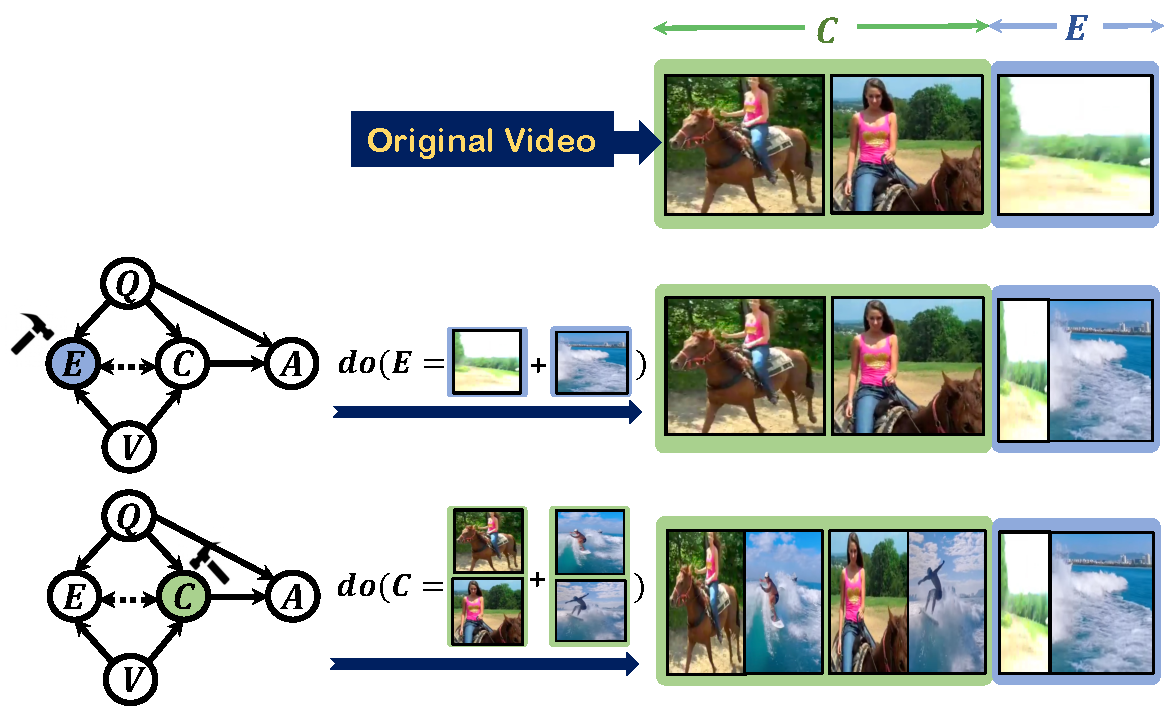
\includegraphics[scale=0.43]{fig/intervene.pdf}
\caption{We illustrate the invariant and equivariant interventions in the second and third rows, respectively. The effects on $Q$ and $A$ are omitted for illustration purposes.}
\vspace{-5pt}
\label{fig:intervene}
\end{figure}
\section{conclusion}
\label{sec:conclusion}
In this paper, we present EIGV --- a model-agnostic explainer, that empowers the SoTA VideoQA model with intrinsic interpretability. In the light of the causality, we formulate our learning principles --- causal-equivariance and environment-invariance by incorporating three constituents, the grounding indicator, the intervener, and the disruptor, which manage a robust rationale discovery. Experiments across three benchmarks validate EIGV's fulfillment in both interpretation and accuracy.

% In addition to the technical advantages, we discuss possible refinements to improve the current design. Unlike some SoTAs that utilize object-level features (\eg HOSTR \cite{dang2021hierarchical} and PGAT \cite{DBLP:conf/mm/PengYBW21}), EIVG merely takes advantage of clip-level representation. Although the architecture of the backbone model is beyond the scope of this work, we anticipate that a fine-grained interpretation at the entity level will strengthen the current EIGV design.
\section{Introduction}
\label{sec:introduction}

\begin{figure}[t]
\centering
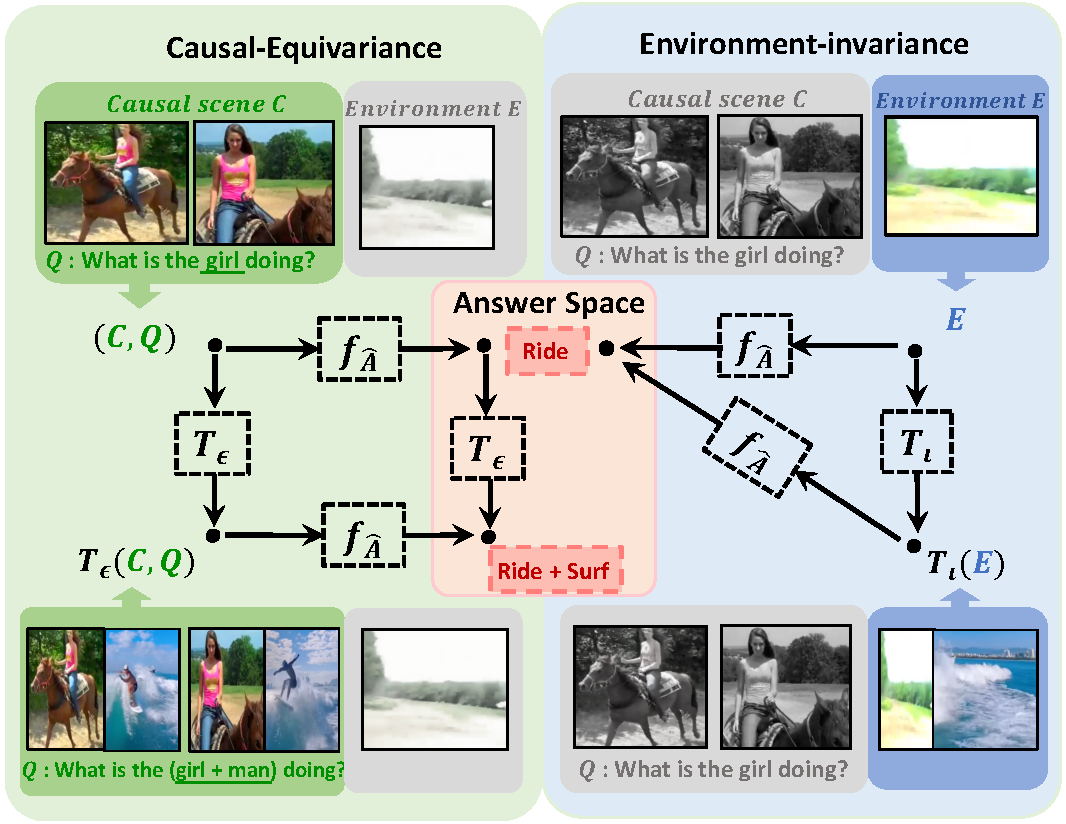
\includegraphics[scale=0.47]{fig/f1.pdf}
\vspace{-15pt}
\caption{
Illustration of equivariant and invariant grounding.
The causal-equivariant principle (left) asks that the semantic change $T_{\epsilon}$ applied to the causal scene $C$ and question $Q$ should be faithfully reflected in the answer change.
In contrast, the environment-invariant principle (right) outputs the same answer, regardless of changes $T_{\iota}$ on the environment scene $E$.
Here, $f_{\hat{A}}$ maps input to answer space.
}
\vspace{-15pt}
\label{fig:overview}
\end{figure}

% 1.videoQA overview-----------------------------------------
Video Question Answering (VideoQA) \cite{zhong2022video} is a keystone in interactive AI, such as vision-language navigation and communication systems.
It aims to answer the natural language question based on the video content.
Striving for the architecture novelty, many studies have been conducted on modeling VideoQA's multi-modal nature, such as fostering the vision-language alignment \cite{jiang2020reasoning,park2021bridge} and revisiting the visual input structure \cite{le2021hierarchical,dang2021hierarchical}.
However, existing VideoQA models usually operate as black boxes, which fail to exhibit the working mechanism behind the predictions and hardly exhibit ``What knowledge should the model use to answer the question about the video?''.
As a result, the black-box nature causes concern for the model's reliability, especially in applications to safety and security.



% 2.problem of interpretable-------------------------------
The concern on the black-box nature calls for  \lyc{better transparency} of VideoQA models.
Here we focus on visual-explainability \cite{CSS,DBLP:conf/ijcai/RossHD17}, aiming to reveal ``Which part of the video should the model look at to answer the question?''.
It requires us to find a subset of visual scenes --- rationale --- \lyc{that support the answering as evidence in way of human interpretation} \cite{DBLP:conf/ijcai/RossHD17}.
Taking Figure \ref{fig:overview} as an example, when answering the question ``What is the girl doing?'', the rationale should focus on the ``girl-riding on-horse'' scene in the first two clips.
Towards this end, existing studies \cite{gao2018motionappearance,DBLP:conf/iccv/Liu0WL21,DBLP:conf/mm/WangG0W21} dwell mainly on the paradigm of \textbf{post-hoc explainability} \cite{LIME,DBLP:conf/iccv/SelvarajuCDVPB17}, which distributes the predictive answer of the target model to the input visual features via an additional explainer method.
They visualize the attention weights or gradient-like signals toward the visual features, and then identify a salient pattern as the rationale.
However, post-hoc explainability has several major limitations:
(1) It fails to make the target model intrinsically interpretable \cite{DBLP:conf/cvpr/YangZQ021,wang2021causal,DBLP:journals/natmi/Rudin19},  only approximating the decision-making process of the model.
As a result, the identified rationale cannot faithfully reveal how the model leverages the multi-modal information.
(2) Such visual inspections are fragile against input perturbations, since some artifacts can be easily captured as explanations instead of genuine knowledge from the data \cite{DBLP:conf/ijcai/LaugelLMRD19,slack2020fooling,heo2019fooling,ghorbani2019interpretation}.




% 3.partition the video to get interpretation ------------
The limitations of post-hoc explainability inspire us to explore the paradigm of \textbf{intrinsic interpretability} \cite{ghorbani2019interpretation,DBLP:journals/natmi/Rudin19}, which embeds a rationalization module into the model to make the decision-making process transparent.
Surprisingly, the intrinsic interpretability of VideoQA models is until-now lacking.
To fill the void, we draw on \textbf{causal theory} \cite{pearl2016causal,pearl2009causal} to formulate the interpretability task as disclosing ``Which part of the video is critical/causal to answering the question?''.
Concretely, we aim to identify the causal component of input video on-the-fly, which holds the question-response information and filters out the question-irrelevant cues.
Following this essence, one straightforward realization is to ground the input video into two segments:
(1) \textbf{causal scene}, which retains the question-critical visual content and sufficiently approaches the answer, thus naturally serving as the rationale;
and (2) \textbf{environment scene}, which holds the question-irrelevant visual content and can be seen as the rationale's complement.



% 4.euiqvariant and invariant -------------------------------
% 要突出的是grounding,title中是Equivariant and invariant grounding,所以要让这些关键词尽早的出现。
% 这个例子融入到下面的Causal-Equivariance和Environmental-Invariance中去。
%
However, discovering causal scene without the supervision of ground-truth rationale is challenging.
With a causal look at the reasoning process (\cf Section \ref{sec:causal-view}), we argue that the crux of intrinsic interpretability is to amplify the connection between the causal scene and the answer, while blocking the non-causal effect of the environment scene.
Following this line, we propose two principles to guide the grounding of the rationale:
\begin{itemize}[leftmargin=*]
    \item \textbf{Causal-Equivariance.}
    By ``equivariance'', we mean that answering should be sensitive to the semantic changes on the causal scene and question (termed E-intervention), \eg any change on the causal scene and question should be faithfully reflected on the predicted answer. For example, in Figure \ref{fig:overview}, the ``girl-riding on-horse'' and ``man-surfing in-ocean'' scenes are the oracle rationales of ``What is the girl doing?'' and ``What is the man doing?'', respectively. The intervention \cite{li2021interventional} applied on the input (\ie mixing the ``girl-riding on-horse'' and ``man-surfing in-ocean'' scene, and combining two questions as ``What is the girl doing? What is the man doing?'') should set off an equivariant change in the answer (\ie changing from ``Ride'' to ``Ride+Surf'').
    
    
    
    \item \textbf{Environment-Invariance.}
    By ``invariance'', we mean that answering should be insensitive to the changes in the environment scene (termed I-intervention), conditioning on the causal scene and question.
    Considering Figure \ref{fig:overview} again, the intervention applied to the environment (\ie mixing the ``meadow'' and ``ocean'' scenes) implies no impact towards answering ``What is the girl doing?'', reflecting a homogeneity in the answer space.
\end{itemize}


%5.overall idea ------------------------------------------------------------------
% Aspiring to capture grounding rationale, we formalize a model-agnostic learning framework, Equivariant and Invariant Grounding for Interpretable VideoQA (EIV), 
% %
% by asking the question ``what and how transformation should the model be equivariant or invariant to?'' 
% %
% Different from the previous effort that design supervised proxy task for geometric transformation \cite{DBLP:conf/iccv/ChengSM21}, 
% % we adopted philosophy of causal intervention and design a saliency-aware temporal mix method for the video input, and impose 
% we answer the ``what'' question by adopting the philosophy of causality \cite{pearl2009causal} and configure transformation as causal intervention operation that imposes scene-aware mixup \cite{DBLP:conf/iclr/ZhangCDL18} on the multi-modal input.
% %
% As for the question of how, we present a unified view of equivariant and invariant principles via the lens of temporal self-supervised learning, where the contrastive counterparts are bred through a disruption on the causal scene, environment scene as well as vision-language alignment.

% where the contrastive counterparts are bred through a disruption on the causal and environment scene, respectively.

% implemetation ----------------------------------------------
% 这一段的写作逻辑应该是如何实现equivariant、invariant principles的;可以不用follow IGV的写法;

% 可以这么组织:
% 一句话介绍三个modules;
% 然后如何用这三个modules来实现两个principle的:首先用grouidng indicator去roughly partition videos into two parts:causal and environmental scenes;然后基于这两部分引入causal-equivariance:利用interventer对于causal scenes做interventions,期望answer部分产生相对应的变化;利用interventer对于environmental scenes做interventions,期待这部分不会对于answering产生影响。

To impose these two principles for intrinsic interpretability, we propose a new framework, \underline{E}quivariant and \underline{I}nvariant \underline{G}rounding for Interpretable \underline{V}ideoQA (\textbf{EIGV}).
EIGV equips the VideoQA backbone model with three additional modules:
a grounding indicator, an intervener, and a disruptor.
First, the grounding indicator learns to attend the causal scene based on the input question, while leaving the rest as the environment.
% However, this grounding only roughly estimates the oracle partition of causal and environment scenes.
Then, the intervener parameterizes the proposed principles to guide the grounding.
Specifically, towards the causal-equivariance principle, it conducts the E-intervention on the causal scene and question --- that is, mix them with the counterparts from another video-question pair --- and encourages the predictive answer to be anticipated accordingly.
Towards the environment-invariance principle, when leaving the causal scene and question untouched, it applies the I-intervention on the environment --- that is, mix it with the environmental stratification of a memory bank --- and enforces the predictive answer to be invariant.
Moreover, we build an unified sight of two principles via the lens of contrastive learning.
Concretely, on top of each intervened video-question pair, the disruptor constructs the positive views by disrupting the environment scene randomly, while creating the negative views by substituting the causal scene with random scenes.
Training with these two principles allows the backbone model to distinguish the causal scene from the environmental cues, and hinge on the critical visual-linguistic alignment. 


Briefly put, our contributions are: 
\begin{itemize}[leftmargin=*]
    \item We propose EIGV, a model-agnostic VideoQA framework that distills the causal visual-linguistic alignment to generate answers in a self-interpretable manner.
    
    \item We investigate the soundness of grounding rationale by posing the equivariant-invariant principle on visual grounding.
    
    \item We justify the superiority of EIGV on three popular benchmark datasets (\ie MSVD-QA \cite{DBLP:conf/mm/XuZX0Z0Z17}, MSRVTT-QA \cite{DBLP:conf/mm/XuZX0Z0Z17},  NExT-QA \cite{DBLP:conf/cvpr/XiaoSYC21}) with extensive experiments, where our design outmatches the state-of-the-art models. Moreover, our EIGV is a model-agnostic framework that can be applied to different VideoQA models. 
\end{itemize}














\section{Related Work}
\label{sec:related}

\begin{figure*}[t]
  \centering
%   \setlength{\abovecaptionskip}{0.cm}
  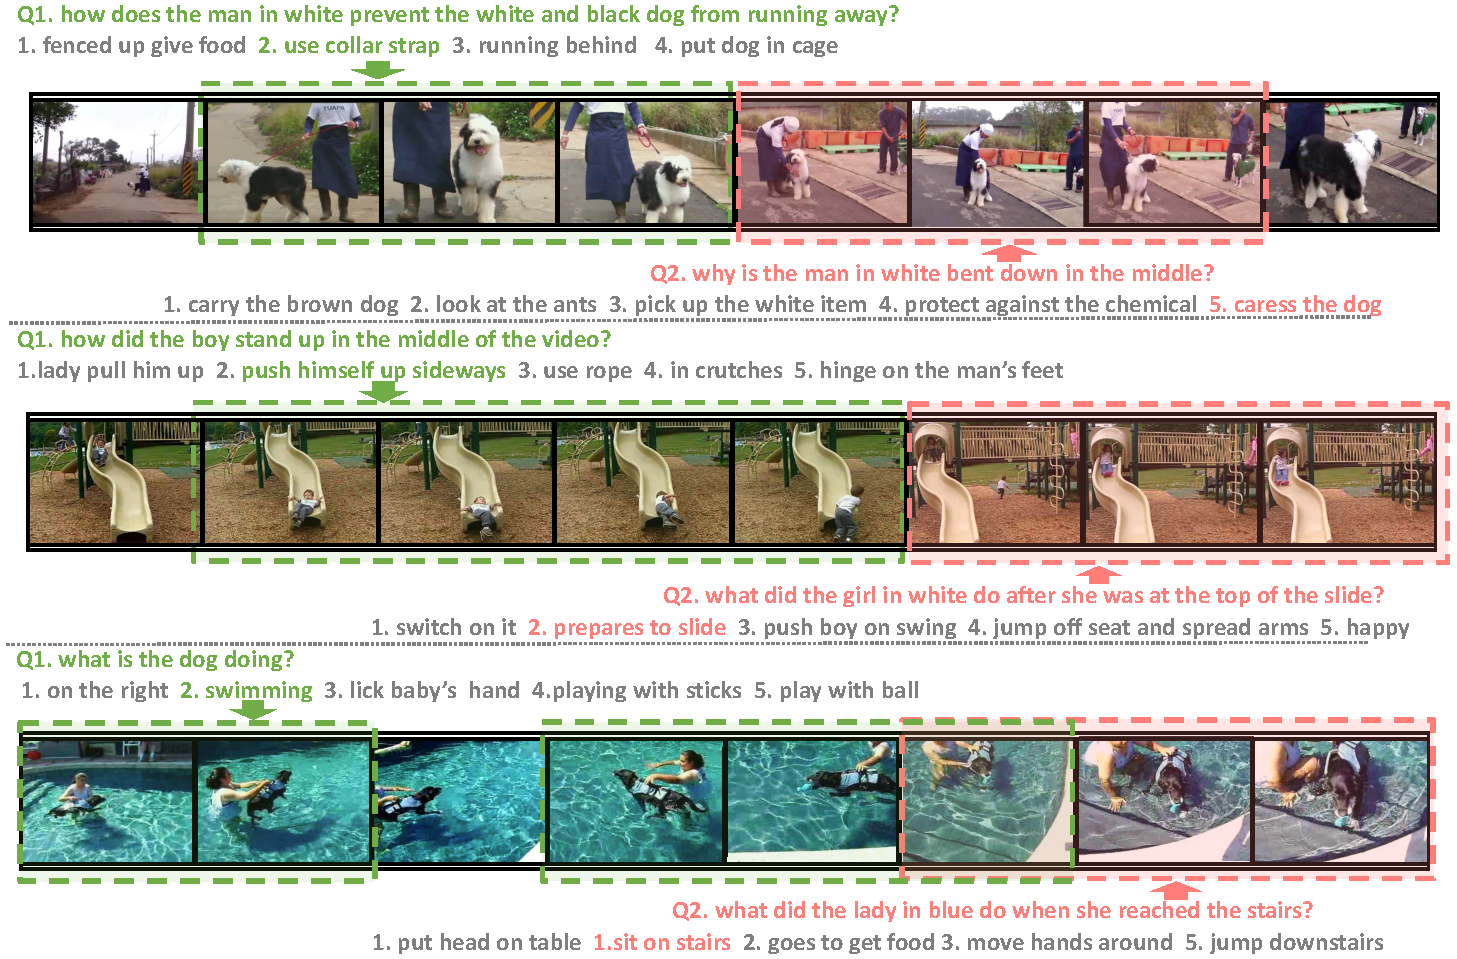
\includegraphics[width=0.97\textwidth]{fig/case.pdf}
 	\vspace{-13pt}
  \caption{Visualization of discovered grounding rationale. Each row comes with a video instance and two questions that target at different scene.  The \textcolor[rgb]{0,0.5,0}{green} and \textcolor[RGB]{225,152,150}{pink} windows indicate the rationales for the corresponding questions.}
  \label{fig:case-study}
 	\vspace{-10pt}
\end{figure*}

\vspace{5pt}
\noindent\textbf{Video Question Answering.}
Established to answer the question in dynamic visual content, VideoQA is bred through the task of ImageQA but has broadened its definition by assembling a temporal dimension. 
%
To make the task intriguing, the VideoQA benchmark has gone beyond the problem of description \cite{DBLP:conf/mm/XuZX0Z0Z17} and built several datasets to challenge temporal reasoning and even causal reflection \cite{DBLP:conf/cvpr/XiaoSYC21}. 
%
As a result, VideoQA has experienced an aggressive expansion in the architecture design. 
% 
Chronologically, early efforts tend to enact alignment through cross-modal attention \cite{zeng2016leveraging,li2019beyond} or enhanced memory design \cite{gao2018motionappearance, DBLP:conf/mm/XuZX0Z0Z17, fan2019heterogeneous}, while more recent works leverage the expressiveness of the graph neural network and perform the relation reasoning as node propagation \cite{jiang2020reasoning, DBLP:conf/mm/PengYBW21} or graph alignment \cite{park2021bridge}. 
%
In addition, current designs modify the representation of video and manipulate the temporal sequence from a hierarchical angle. Following this line, HCRN \cite{le2021hierarchical} first came out with the conditional relation module as building blocks that operate through different video intervals, whereas  HOSTR and PGAT made their advancement by incorporating visual content from different granularity. MSPAN, however, established cross-scale feature interaction on top of the hierarchy.
%
Despite effective, their intrinsic rationale has long been overlooked. To the best of our knowledge, EIGV is the first work that probes intrinsic interpretation. 

\vspace{5pt}
\noindent\textbf{Invariant Learning.}
% Given a encoder $f(\cdot)$ and input $x$, a representation $f(x)$ is equivariant to operation $G$, if $\forall x : f(G(x)) = T(G(x))$ ; Likewise, the property of invariance is defined as $\forall x : f(G(x)) = f(x)$. 
Given a encoder $f(\cdot)$ and input $x$, a representation $f(x)$ is invariant to operation $T$, if $\forall x : f(G(x)) = f(x)$. 
%
In practice, this invariant property has a long history in presenting visual content (\eg HOG \cite{DBLP:conf/mmm/HuangTHTJ11}), which has recently been renovated by deep learning in form of risk minimization. As its most prevailing form, IRM \cite{arjovsky2020invariant} fosters this philosophy by posing an environment invariant prior and discovering the underlying causal pattern by reducing cross-environment variance.   
% .that remains stable across different environments.
Different from previous studies that create environment via inductive re-grouping \cite{DBLP:conf/cvpr/AndersonWTB0S0G18} or adversarial inference \cite{DBLP:conf/icml/CreagerJZ21,wang2021causal, wang2022causal,wang2021clicks}, our method conducts causal intervention that perturbs the original sample distribution to form a new one.
\lyc{The most relvant work is \cite{Li_2022_CVPR}, where an invariant framework is introduced as a model-agnostic framework. However, EIGV gains better generalization ability by marrying equivariance as complementary learning principle.}
% Specifically, the discovery of  rationale implies two requirements on the partition:

\vspace{5pt}
\noindent\textbf{Visual Interpretability}
Machine interpretability can be achieved in various methods, such as clustering \cite{monnier2020dticlustering} or disentanglement \cite{shen2020interfacegan}. Our design can be vested in the category of attribution discovery, which investigates the contribution of different input elements toward the prediction. 
Based on whether the prediction and interpretation are yielded simultaneously, two categories are further defined: 1) post-hoc methods that generated the interpretation after prediction, such as backpropagation methods (\eg grad-CAM \cite{DBLP:conf/iccv/SelvarajuCDVPB17}). 2) self-interpretable method that cast prediction and interpretation at the same stage.
%
Unlike the post-hoc method that traces the interpretative clue from the output of the black-box, the self-interpretable model builds a transparency model via methods such as prototype generation \cite{DBLP:journals/corr/abs-1806-10574} or structural delineation \cite{wu2022dir}. 
%
In fact, previous works tend to focus on static image. EIGV, however, approaches the video interpretation in a multi-modal situation. 

\vspace{-5pt}
\section{Limitation and Complexity}
\label{section:limits}
\lyc{In addition to the technical advantages, we discuss possible limits of the current design. Unlike some SoTAs that utilize object-level features (\eg HOSTR \cite{dang2021hierarchical} and PGAT \cite{DBLP:conf/mm/PengYBW21}), EIVG merely takes advantage of clip-level representation. Although the architecture of the backbone model is beyond the scope of this work, we anticipate that a fine-grained interpretation at the entity level will strengthen the current EIGV design.
% 2) Current intervention strategy can possibly threaten the causal prediction by introducing context with new shortcuts. Since the scene intervener sample context stratification in a random manner, there is a slight chance to draw an undesired substitute that nested with strong static relation towards  a wrong answer, thus inducing a false prediction.
In terms of complexity, we run all experiments on NVIDIA Tesla V100 GPU, where our algorithm matched equally with the corresponding baseline.  For comparison, the backbone MSPAN model is trained for 1.5 hours till convergence on NExT-QA, whereas EIGV 
takes 1.6 hours.
}
% Table generated by Excel2LaTeX from sheet 'Sheet1'
\begin{table}[t]
  \centering
  \caption{Evaluation on the effectiveness of sub-modules}
    \resizebox{0.9\linewidth}{!}{
    \begin{tabular}{c|cc|cc}
    \toprule
    \multirow{2}[2]{*}{Ablation} & \multicolumn{2}{c|}{MSVD-QA} & \multicolumn{2}{c}{NExT-QA} \\
          & MSPAN & HGA   & MSPAN & HGA \\
    \midrule
    \midrule
    SoTA Backbone & 40.3  & 36.6  & 50.7  & 50.0 \\
    \midrule
    $+$ Mixup \cite{DBLP:conf/iclr/ZhangCDL18} & 41.0    & 38.3  & 52.0    & 51.8 \\
    $+$ Intervener & 41.5  & 39.6  & 52.5  & 52.7 \\
    \midrule
    $+$ Disruptor & 40.9  & 37.6  & 51.0    & 51.1 \\
    \white{66666} $+$ Disrupt-Q & 40.6  & 37.0    & 50.8  & 51.0 \\
    \white{66666} $+$ Disrupt-V & 40.7  & 37.3  & 51.0    & 50.8 \\
    \midrule
    EIGV & \textbf{42.6} & \textbf{40.8} & \textbf{52.9} & \textbf{53.7} \\
    \bottomrule
    \end{tabular}%
    }
    \vspace{-15pt}
  \label{tab:ablation}%
\end{table}%

% Table generated by Excel2LaTeX from sheet 'Sheet1'
\begin{table}[t]
  \centering
  \caption{Comparison with SoTAs. Our results are highlighted.}
    \resizebox{0.95\linewidth}{!}{
    \begin{tabular}{cc|ccc}
    \toprule
          & Model & MSVD-QA & MSRVTT-QA & NExT-QA \\
    \midrule
    \midrule
    \multirow{9}[6]{*}{\rot{SoTAs}} & AMU \cite{DBLP:conf/mm/XuZX0Z0Z17}   & 32.0    & 32.0    & - \\
          & HME \cite{fan2019heterogeneous} \  & 33.7  & 33.0    & 49.2 \\
\cmidrule{2-5}          & B2A  \cite{park2021bridge}   & 37.2  & 36.9  & - \\
          & L-GCN \cite{huang2020locationaware} & 34.3  & 33.7  & 49.5 \\
\cmidrule{2-5}          & HCRN \cite{le2021hierarchical}  & 36.1  & 35.6  & 48.9 \\
          & PGAT \cite{DBLP:conf/mm/PengYBW21} & 39.0    & 38.1  & - \\
          & HOSTR \cite{dang2021hierarchical} & 39.4  & 35.9  & - \\
          & \lyc{HQGA} \cite{xiao2021video} & \underline{41.2}  & \underline{38.6}  & \underline{51.8} \\
\cmidrule{2-5} & \lyc{IGV} \cite{Li_2022_CVPR} & 40.8  & 38.3  & 51.3 \\
    \midrule
    \midrule
    \multirow{6}[6]{*}{\rot{Ours}} & Co-Mem \cite{gao2018motionappearance}& 34.6  & 35.3  & 48.5 \\
          & \white{66666}$+$ EIGV   & \cellcolor[rgb]{ .851,  .851,  .851}         \textcolor{gray}{666}39.8 $^{\imp{+5.2}}$ & \cellcolor[rgb]{ .851,  .851,  .851} \textcolor{gray}{666}37.2 $^{\imp{+1.9}}$ & \cellcolor[rgb]{ .851,  .851,  .851} \textcolor{gray}{666}50.7 $^{\imp{+2.2}}$ \\
\cmidrule{2-5}          &  HGA \cite{jiang2020reasoning}   & 36.6  & 36.7  & 50.0 \\
          & \white{66666}$+$ EIGV   & \cellcolor[rgb]{ .851,  .851,  .851} \textcolor{gray}{666}40.8 $^{\imp{+4.2}}$& \cellcolor[rgb]{ .851,  .851,  .851} \textcolor{gray}{666}38.5 $^{\imp{+1.8}}$ & \cellcolor[rgb]{ .851,  .851,  .851} \textcolor{gray}{666}\textbf{53.7} $^{\imp{+3.7}}$ \\
\cmidrule{2-5}          & MSPAN \cite{DBLP:conf/acl/GuoZJ0L20} & 40.3  & 38.0    & 50.7 \\
          & \white{66666}$+$ EIGV   & \cellcolor[rgb]{ .851,  .851,  .851} \textcolor{gray}{666}\textbf{42.6} $^{\imp{+2.3}}$ & \cellcolor[rgb]{ .851,  .851,  .851} \textcolor{gray}{666}\textbf{39.3} $^{\imp{+1.3}}$ & \cellcolor[rgb]{ .851,  .851,  .851} \textcolor{gray}{666}52.9 $^{\imp{+2.2}}$ \\
    \bottomrule
    \end{tabular}%
    }
    \vspace{-5pt}
  \label{tab:main}%
\end{table}%

% Table generated by Excel2LaTeX from sheet 'Sheet1'
\begin{table}[t]
  \centering
  \caption{Study of feature setting. ``APP'' and ``MOT'' denotes using appearance and motion feature individually. }
    \resizebox{0.95\linewidth}{!}{
    \begin{tabular}{cc|cc|cc}
    \toprule
    \multicolumn{2}{c|}{\multirow{2}[2]{*}{Method}} & \multicolumn{2}{c|}{MSVD-QA} & \multicolumn{2}{c}{NExT-QA} \\
    \multicolumn{2}{c|}{} & MSPAN & HGA   & MSPAN & HGA \\
    \midrule
    \midrule
    \multirow{2}[2]{*}{\rot{APP}} & SoTA Backbone & 40.1  & 35.0    & 49.7  & 48.3 \\
          & \white{66666}$+$ EIGV   & \textbf{41.0}    & \textbf{39.5}  & \textbf{52.0}    & \textbf{52.4} \\
    \midrule
    \multirow{2}[2]{*}{\rot{MOT}} & SoTA Backbone & 37.8  & 33.6  & 49.4  & 47.5 \\
          & \white{66666}$+$ EIGV   & \textbf{39.3}  & \textbf{38.5}  & \textbf{51.1}  & \textbf{51.7} \\
    \bottomrule
    \end{tabular}%
    }
  \vspace{-15pt}
  \label{tab:unifeat}%
\end{table}%




\section{Introduction}
\label{sec:introduction}


% 1.videoQA overview-----------------------------------------
% 第一段介绍背景:
% 一句话介绍VideoQA的重要性;
% 一句话介绍VideoQA的task;
% 然后引出现有VideoQA models都是black-box的困扰;
% 2-3句话介绍black-box的坏处是啥。

\wx{Video Question Answering (VideoQA) \cite{fan2019heterogeneous} is a keystone in interactive AI, such as vision-language navigation and communication systems.
It aims to answer the natural language question based on the video content.
Nourished by the multi-modal nature, VideoQA \emph{per se} has relished an expansion in the model design, which spans from fostering the vision-language alignment \cite{jiang2020reasoning,park2021bridge} to revisiting the visual input structure \cite{le2021hierarchical,dang2021hierarchical}.
However, existing VideoQA models usually work as black boxes, which fail to exhibit the working mechanism behind the predictions and hardly reveal ``What knowledge should the model use to answer the question about the video?''.
% However, existing VideoQA models usually work as black boxes, which fail to exhibit the intrinsic rationale behind the predictions and hardly answer ``What knowledge should the model use to answer the question about the video?''.
As a result, the black-box nature causes concern for the model reliability and hinders the model deployment, especially in applications on safety and security.

}

% More frustratingly, the system gives
% no hint about which part of such systems is the
% culprit for a wrong answer

\begin{figure}[t]
\centering
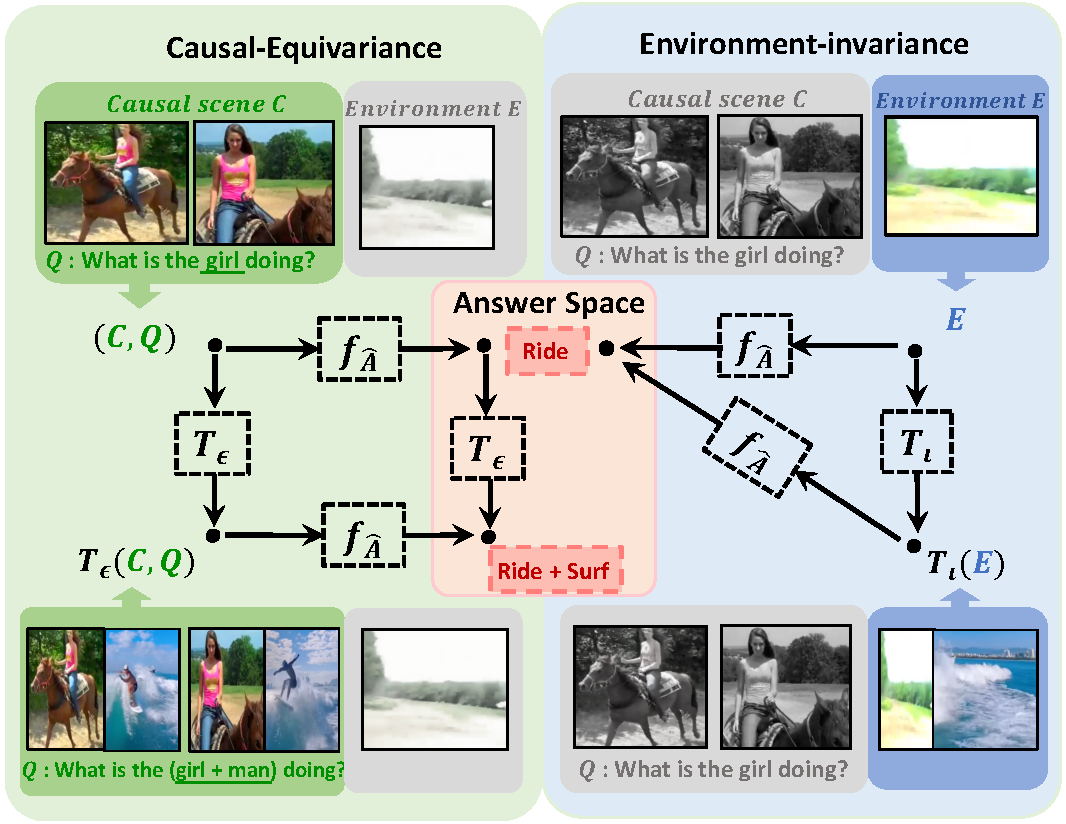
\includegraphics[scale=0.47]{fig/f1.pdf}
\caption{Illustration of causal-equivariant and environment-invariant principles, where $C,E$ are the causal and environment of input video, $f_{\hat{A}}$ is a map from input space to answer space, $T_{\epsilon}$ and $T_{\iota}$ are transformations (instantiated as a mixture of two data points) that applies to causal and non-causal factors, respectively.}
% (\textcolor[rgb]{0,0.5,0}{Green}: causal-equivarince; \textcolor[rgb]{0.03,0.27,0.49}{Navy}: complement-invariance)}
\vspace{-18pt}
\label{fig:overview}
\end{figure}


% 2.problem of interpretable-------------------------------
% 第二段介绍explainability/interpretability in VideoQA:
% 一句话描述:对于black-box nature的concerns,explainability in VideoQA非常重要;
% 一句话描述:explainability in VideoQA是要回答什么问题:which part of the video should the model look at to answer the question?
% 然后说明现在都是post-hoc explanations,这里要点出来post-hoc的基本概念是啥;然后一两句话介绍post-hoc为啥有缺陷。


% \wx{
% The concern on the black-box nature calls for explainability of VideoQA models.
% Here we focus on visual-explainability \cite{CSS,DBLP:conf/ijcai/RossHD17}, aiming to answer ``Which part of the video should the model look at to answer the question?''.
% It inspires us to ground a subset of visual scenes --- rationale --- which are the right reasons for the right answering \cite{DBLP:conf/ijcai/RossHD17}.
% Towards this end, the current studies \cite{gao2018motionappearance,DBLP:conf/iccv/Liu0WL21,10.1145/3474085.3475620} dwell on the ``learning to attend'' paradigm \cite{DBLP:conf/nips/VaswaniSPUJGKP17,DBLP:conf/icml/XuBKCCSZB15}, which uses the attention mechanism to identify some informative scenes as the explanation.
% To optimize the attention mechanism, empirical risk minimization (ERM)
% }


\wx{
The concern on the black-box nature calls for explainability of VideoQA models.
Here we focus on visual-explainability \cite{CSS,DBLP:conf/ijcai/RossHD17}, aiming to reveal ``Which part of the video should the model look at to answer the question?''.
It requires us to find a subset of visual scenes --- rationale --- which are the right reasons for the right answering \cite{DBLP:conf/ijcai/RossHD17}.
Taking Figure \ref{fig:overview} as an example, when answering the question ``What is the girl doing?'', the rationale should focus on the ``girl-riding on-horse'' scene in the first two clips.
% Towards this end, there are two prevalent paradigms: post-hoc explainability, intrinsic interpretability.
Towards this end, the current studies \cite{gao2018motionappearance,DBLP:conf/iccv/Liu0WL21,10.1145/3474085.3475620} dwell mainly on the paradigm of \textbf{post-hoc explainability} \cite{LIME,DBLP:conf/iccv/SelvarajuCDVPB17}, which distributes the target model's predicted answer to the input visual features via an additional explainer method.
They visualize the attention weights or gradient-like signals about the visual features, and then identify a salient pattern as the rationale.
However, post-hoc explainability has several major limitations:
(1) It fails to make the target model intrinsically interpretable \cite{DBLP:conf/cvpr/YangZQ021,DBLP:conf/iccv/WangZSZ21}, only approximating the decision-making process of the model.
As a result, the identified rationale cannot faithfully reveal how the model leverages the multi-modal information.
(2) Such visual inspections are fragile against input perturbations, since some artifacts can be easily captured as explanations instead of genuine knowledge from the data \cite{DBLP:conf/ijcai/LaugelLMRD19,slack2020fooling,heo2019fooling,ghorbani2019interpretation}.
}


% Trust concern on the black-box nature of existing methods calls upon a comprehensive study on model interpretability, \ie how they arrive at a specific prediction. 
% %
% In the context of the VideoQA, a favorable interpretation ought to answer the million-dollar question "which part of the video should the model look at to answer the question?" 
% %
% Despite the necessity, the explainability of the current design still dwells on the post-hoc paradigm \cite{gao2018motionappearance,DBLP:conf/iccv/Liu0WL21,10.1145/3474085.3475620}, where interpretations are approximated by extracting a salience pattern from the trained predictive model without any inductive knowledge ( \eg visualize attention weight).
% %
% Unfortunately, the visual justification via the post-hoc method is fragile against input perturbations, since some artifacts can be easily captured as explanations instead of genuine knowledge from the data \cite{DBLP:conf/ijcai/LaugelLMRD19,slack2020fooling,heo2019fooling,ghorbani2019interpretation}. As a result, peeking through output (\za{\eg LIME \cite{LIME}}, Grad-CAM \cite{DBLP:conf/iccv/SelvarajuCDVPB17}) cannot faithfully reveal how machine leverage the multi-modal information, which left our million-dollar concern unaddressed.

% which is fragile against input perturbations, and less instructive to the predictive mechanism. 


% In addition, it is debatable whether attention mechanisms are indeed explanations (Wiegreffe and Pinter, 2019; Jain and Wallace, 2019). M

% Worse still, overwhelming computational power has provoked the model complexity with billions of parameters, which, as a seed of distrust, shadowed the model's transparency along with our faith. 
%


% 3.partition the video to get interpretation ------------
% 第三段讲我们要研究的内容:
% 一句话介绍我们关注intrinsic interpretability,但是研究的人很少;
% 一句话描述我们的self-interpretable问题是“which part of the video is critical/causal to answering the question?”
% 然后引出我们要把visual scenes分成两部分一部分是causal scene,一部分是environmental scenes:分别介绍这两个具有啥子semantics。

\wx{The limitations of post-ho explainability inspire us to explore the paradigm of \textbf{intrinsic interpretability} \cite{ghorbani2019interpretation}, which implants a rationalization module into the model to make the decision-making process transparent.
Surprisingly, intrinsic interpretability of VideoQA models is until-now lacking but our focus in this work.
To fill the void, we draw on \textbf{causal theory} \cite{pearl2016causal,pearl2009causal} to formulate the interpretability task as answering ``Which part of the video is critical/causal to answering the question?''.
Concretely, we aim to identify the causal component of input video on-the-fly, which holds the question-response information and filters the question-irrelevant cues out.
Following this essence, one straightforward realization is to ground the input video into two segments:
(1) \textbf{causal scene}, which retains the question-critical visual content and sufficiently approaches the answer, thus naturally serving as the rationale;
(2) \textbf{environment scene}, which holds the question-irrelevant visual content and can be seen as the rationale's complement.
}



% 4.euiqvariant and invariant -------------------------------
% 要突出的是grounding,title中是Equivariant and invariant grounding,所以要让这些关键词尽早的出现。
% 这个例子融入到下面的Causal-Equivariance和Environmental-Invariance中去。
%
\wx{However, discovering causal scene without the supervision of ground-truth rationale is challenging.
With a causal look at the reasoning process (\cf Section \ref{sec:causal-view}), we argue the crux of intrinsic interpretability is to amplify the connection between the causal scene and the answer, while blocking the non-causal effect of the environment scene.
Following this line, we propose two principles to guide the grounding of the rationale:}
\begin{itemize}[leftmargin=*]
    \item \textbf{Causal-Equivariance.}
    \wx{By ``equivariance'', we mean that answering should be sensitive to the semantic changes on the causal scene and question (termed E-intervention), \eg any change on the causal scene and question should be faithfully reflected on the predicted answer. For example, the ``girl-riding on-horse'' and \lyc{``man-surfing in-ocean''} scenes are the oracle rationales of ``What is the girl doing?'' and ``What is the man doing?'', respectively. The intervention applied on the input (\ie mixing the ``girl-riding on-horse'' and \lyc{``man-surfing in-ocean''} scene, and combining two questions as ``What is the girl doing? What is the man doing?'') should set off an equivariant change in the answer (\ie changing from ``Ride'' to ``Ride+\lyc{Surf}'').
    }
    
    
    % In essence, transformation on the causal scene should cause the parallel change on the representation manifold. By introspecting ``How would the predictive answer vary if the causal scenes change?'', the grounding mechanism is aware of the transformations and thus maintains the predictive interpretation.
    % %
    % As exemplified in Figure \ref{fig:overview}, equivariance implies that transformation applied to question-critic information (\ie causal scene and question) should set off an equivariant semantic change in answer space.
    % %
    % Correspondingly, a cautious formulation of such co-variation should help the model pinpoint the 'girl-on-horse' scene as a grounding rationale for ``ride''.
    
    \item \textbf{Environment-Invariance.}
    \wx{By ``invariance'', we mean that answering should be insensitive to the changes in the environment (termed I-intervention), conditioning on the causal scene and question.
    Considering Figure \ref{fig:overview} again, the intervention applied on the environment (\ie mixing the ``meadow'' and \lyc{``ocean''} scenes) implies no impact towards answering ``What is the girl doing?'', reflecting a homogeneity in the answer space.
    }

    
    % % 是它不符合human cognition以及它会产生spurious correlation
    % On the ground of the prophet, permutation on environment scene should be invariant to predictive answer, since environment implies no impact to the predictive answer except spurious correlation, comprising it as rationale runs counter to the human cognition. 
    % % On ground of the prophet, the predictive answer is invariant against permutation on environment scene, as it does not contribute to the reasoning mechanism or interpretation.
    % %
    % Consider the example in Figure \ref{fig:overview} again, since an environment like ``landscape'' provides no evidence toward the answer ``ride'', its corresponding transformation should reflect a homogeneity in the answer space. The invariance principle epitomizes such assumption by ruling a transformation that is in-vary to answer permutation.
\end{itemize}


%5.overall idea ------------------------------------------------------------------
% Aspiring to capture grounding rationale, we formalize a model-agnostic learning framework, Equivariant and Invariant Grounding for Interpretable VideoQA (EIV), 
% %
% by asking the question ``what and how transformation should the model be equivariant or invariant to?'' 
% %
% Different from the previous effort that design supervised proxy task for geometric transformation \cite{DBLP:conf/iccv/ChengSM21}, 
% % we adopted philosophy of causal intervention and design a saliency-aware temporal mix method for the video input, and impose 
% we answer the ``what'' question by adopting the philosophy of causality \cite{pearl2009causal} and configure transformation as causal intervention operation that imposes scene-aware mixup \cite{DBLP:conf/iclr/ZhangCDL18} on the multi-modal input.
% %
% As for the question of how, we present a unified view of equivariant and invariant principles via the lens of temporal self-supervised learning, where the contrastive counterparts are bred through a disruption on the causal scene, environment scene as well as vision-language alignment.

% where the contrastive counterparts are bred through a disruption on the causal and environment scene, respectively.

% implemetation ----------------------------------------------
% 这一段的写作逻辑应该是如何实现equivariant、invariant principles的;可以不用follow IGV的写法;

% 可以这么组织:
% 一句话介绍三个modules;
% 然后如何用这三个modules来实现两个principle的:首先用grouidng indicator去roughly partition videos into two parts:causal and environmental scenes;然后基于这两部分引入causal-equivariance:利用interventer对于causal scenes做interventions,期望answer部分产生相对应的变化;利用interventer对于environmental scenes做interventions,期待这部分不会对于answering产生影响。

\wx{To impose these two principles for intrinsic interpretability, we propose a new framework, \underline{E}quivariant and \underline{I}nvariant \underline{G}rounding for Interpretable \underline{V}ideoQA (\textbf{EIGV}).
EIGV equips the VideoQA backbone model with three additional modules:
a grounding indicator, an intervener, and a disruptor.
First, the grounding indicator learns to attend the causal scene based on the input question, while leaving the rest as the environment.
% However, this grounding only roughly estimates the oracle partition of causal and environment scenes.
Then, the intervener parameterizes these principles to guide the grounding.
Specifically, towards the causal-equivariance principle, it conducts the E-intervention on the causal scene and question --- that is, mix them with the counterparts from another video-question pair --- and encourages the answering to be anticipated accordingly.
Towards the environment-invariance principle, when leaving the causal scene and question untouched, it applies the I-intervention on the environment --- that is, mix it with the environmental stratification of a memory bank --- and enforces the predicted answer to be invariant.
On the top of intervened video-question pairs, the disruptor constructs the contrastive twins.
}


% In light of the proposed princes, we formalize EIGV (\underline{E}quivariant and \underline{I}nvariant \underline{G}rounding for Interpretable \underline{V}ideoQA),
% a model-agnostic explainer to capture the stable visual rationale VideoQA models.
% % 一句话介绍三个modules;
% Specifically, EGV absorbs three modules in addition to the backbone VideoQA model: a grounding indicator, an intervener, and a disruptor. 
%
%grounding indicator
In particular, the grounding indicator learns to separate the causal scenes as the interpretation and leave the rest as the environment. 
%
% causal-equivariance
Then, for the causal scene of interest, an intervener imposes the equivariance principle via a convex combination of two data points, while anticipating a corresponding change in the answer space.  
%
% environment-invariance
As for the environment counterpart, the invariant principle is realized using a similar intervener, but expecting an unchanged answer.
% %
% Noticeably, since mixing environment does not affect the reasoning dynamics, the answer is modified with the same ratio as the causal scene but independent to environmental one. 
%
% By capturing the equivariance from the answer to the causal scene and the invariance to environment, the model perceives a faithful interpretation that preserves the predictive mechanism.
%
On top of the intervened video, we present a unified view of equivariant and invariant principles via the lens of temporal self-supervised learning. 
%
Concretely, a disruptor substitutes the environment and causal scene with the stratification sampled from a memory bank (a collection of other training videos) to constitute the contrastive twins, respectively. 
%
% To fortify visual-question pair-wise cohesiveness, we also develops alternatives in addition to visual negatives by disrupting the visual-question coupling.
%
In addition to the visual negatives, we also develop alternatives by disrupting the visual-question coupling, to fortify their pair-wise cohesiveness.

% where the contrastive counterparts are bred through a disruption on the causal scene, environment scene as well as vision-language alignment.

% On top of the intervened video, the disruptor substitutes the complement scene with the stratification sampled from a memory bank (a collection of other training videos) and constitutes the “counterfactual video” as the positive sample.
% Likewise, the negative sample is constructed via replacement on the causal scene. 
% %
% In addition to the visual negatives that ``disrupt'' the causal scene, the disruptor also develops alternatives by disrupting the visual-question coupling, to fortify their pair-wise cohesiveness.
% 
After acquiring anchor representation alongside its contrastive twins, the auxiliary contrastive objective reveals the discriminative representation purely from the scene of interest, thus fostering the robustness of interpretation.

Briefly put, our contributions are: 
\begin{itemize}[leftmargin=*]
    \item We propose EGV, a model-agnostic VideoQA explainer that captures the intrinsic causal pattern in a self-interpretable manner.
    
    \item We investigate the soundness of grounding rationale by posing the equivariant-invariant principle on visual grounding and realize it via the causal instrument.
    
    \item We justify the superiority of EGV on three popular benchmark datasets (\ie MSVD-QA \cite{DBLP:conf/mm/XuZX0Z0Z17}, MSRVTT-QA \cite{DBLP:conf/mm/XuZX0Z0Z17},  NExT-QA \cite{DBLP:conf/cvpr/XiaoSYC21}) with extensive experiments, where our design outmatches all the state-of-the-art models.
\end{itemize}














\section{Introduction}
\label{sec:introduction}


% 1.videoQA overview-----------------------------------------
% 第一段介绍背景:
% 一句话介绍VideoQA的重要性;
% 一句话介绍VideoQA的task;
% 然后引出现有VideoQA models都是black-box的困扰;
% 2-3句话介绍black-box的坏处是啥。

\wx{Video Question Answering (VideoQA) \cite{fan2019heterogeneous} is a keystone in interactive AI, such as vision-language navigation and communication systems.
It aims to answer the natural language question based on the video content.}


In pursuance of interactive AI, Video Question Answering (VideoQA) \cite{fan2019heterogeneous} serves as a keystone in abridging human cognition and machine intelligence, whose goal is to answer the natural language question based on the video content.   
%
Nourished by its multi-modal nature, VideoQA \textit{per se} has relished an overwhelming expansion in model design, which either fosters the vision-language alignment \cite{jiang2020reasoning,park2021bridge} or revisit the visual input structure \cite{le2021hierarchical,dang2021hierarchical}.
%
Albeit their sterling performance, existing solutions are usually expressed as black boxes, where the intrinsic rationale --- how to identify the question-responsive visual elements, is still clouded from our intuition. 
%
As a result, such opaqueness certainly raises reliability concern when the model is deployed in the real-word application, such as \ie intelligent surveillant assistant or more generally, an out-of-distribution test setting.

% More frustratingly, the system gives
% no hint about which part of such systems is the
% culprit for a wrong answer

\begin{figure}[t]
\centering
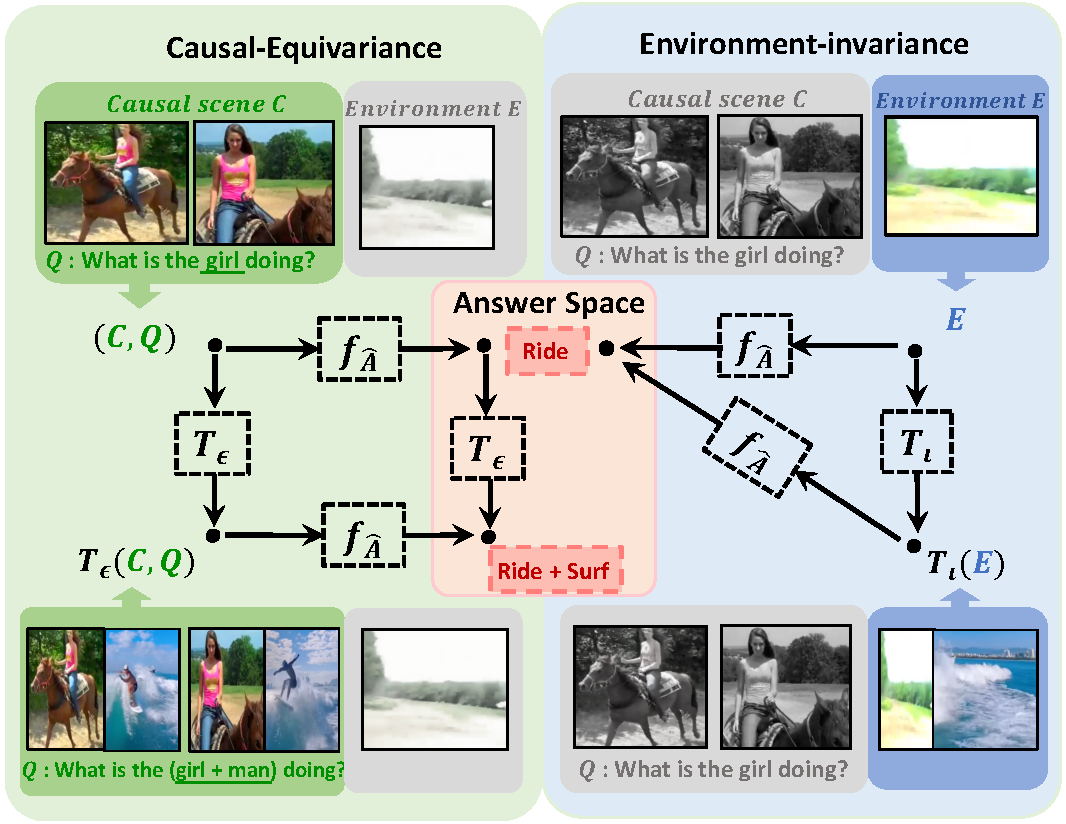
\includegraphics[scale=0.53]{fig/f1.pdf}
\caption{Illustration of causal-equivariant and environment-invariant principle, where $x$ is the input video-question pair, $f$ is a map from input space to answer space, $T$ is a transformation operator that applies to both input and answer space}.
% (\textcolor[rgb]{0,0.5,0}{Green}: causal-equivarince; \textcolor[rgb]{0.03,0.27,0.49}{Navy}: complement-invariance)}
\vspace{-5pt}
\label{fig:overview}
\end{figure}


% 2.problem of interpretable-------------------------------
% 第二段介绍explainability/interpretability in VideoQA:
% 一句话描述:对于black-box nature的concerns,explainability in VideoQA非常重要;
% 一句话描述:explainability in VideoQA是要回答什么问题:which part of the video should the model look at to answer the question?
% 然后说明现在都是post-hoc explanations,这里要点出来post-hoc的基本概念是啥;然后一两句话介绍post-hoc为啥有缺陷。

Trust concern on the black-box nature of existing methods calls upon a comprehensive study on model interpretability, \ie how they arrive at a specific prediction. 
%
In the context of the VideoQA, a favorable interpretation ought to answer the million-dollar question "which part of the video should the model look at to answer the question?" 
%
Despite the necessity, the explainability of the current design still dwells on the post-hoc paradigm \cite{gao2018motionappearance,DBLP:conf/iccv/Liu0WL21,10.1145/3474085.3475620}, where interpretations are approximated by extracting a salience pattern from the trained predictive model without any inductive knowledge ( \eg visualize attention weight).
%
Unfortunately, the visual justification via the post-hoc method is fragile against input perturbations, since some artifacts can be easily captured as explanations instead of genuine knowledge from the data \cite{DBLP:conf/ijcai/LaugelLMRD19}. As a result, peeking through output (\ie Grad-CAM \cite{DBLP:conf/iccv/SelvarajuCDVPB17}) is implicit and cannot faithful reveals how machine leverage the multi-modal information, which left our million-dollar concern unaddressed.

% which is fragile against input perturbations, and less instructive to the predictive mechanism. 


% In addition, it is debatable whether attention mechanisms are indeed explanations (Wiegreffe and Pinter, 2019; Jain and Wallace, 2019). M

% Worse still, overwhelming computational power has provoked the model complexity with billions of parameters, which, as a seed of distrust, shadowed the model's transparency along with our faith. 
%


% 3.partition the video to get interpretation ------------
% 第三段讲我们要研究的内容:
% 一句话介绍我们关注intrinsic interpretability,但是研究的人很少;
% 一句话描述我们的self-interpretable问题是“which part of the video is critical/causal to answering the question?”
% 然后引出我们要把visual scenes分成两部分一部分是causal scene,一部分是environmental scenes:分别介绍这两个具有啥子semantics。

Clearly, inferring a reliable rationale requires intrinsic interpretability to illuminate the reasoning insight. 
%
However essential, a self-interpretable VideoQA explainer that reveals such intrinsic prediction mechanism is until-now lacking.
%
To fill this gap, we get inspiration from \textit{causal theory} \cite{pearl2016causal} and capture such self-interpretability by answering the question of gold --- ``which part of the video is critical/causal to answering the question?'' 
% 
Concretely, we aim to find the causal part of input video on-the-fly that preserves the maximum visual information toward the question, whose discovery will justify the prediction and encourage the generalization.
%
Following this essence, one straightforward realization is to empower the model with discernment that grounds the visual scene into two segments: 
(1) \textbf{causal scene} that retains the question-critical video content and preserves all the relevant information about the target answer, which naturally serves as interpretation for the prediction; (2) \textbf{environment scene} that holds answer-irrelevant environment information of input video. 

% To the best of our knowledge, a self-interpretable VideoQA explainer that reveals the intrinsic prediction mechanism is critical to trustworthy videoQA but until-now lacking.
%

% Clearly, inferring a reliable answer requires a grounding rationale of the prediction, \ie to answer the million-dollar question "which part of the video scene should  be looking at?". 
%
% Inspired by the information bottleneck, which tends to reduce the overload of information processing \cite{DBLP:conf/iclr/SaxeBDAKTC18}, we aim to find the causal for input video that preserves the maximum visual information toward the question, whose discovery will justify the prediction and increase the generalization. 

%
% Following this essence, one straightforward solution is to empower the model with discernment that splits the visual scene into two segments: 
% (1) \textbf{causal scene} that retains the question-critical video content and preserving all the relevant information about the target answer, which naturally serves as interpretation for the prediction; (2) \textbf{environment scene} that holds answer-irrelevant environment information of input video. 


% 4.euiqvariant and invariant -------------------------------
% 要突出的是grounding,title中是Equivariant and invariant grounding,所以要让这些关键词尽早的出现。
% 这个例子融入到下面的Causal-Equivariance和Environmental-Invariance中去。
%
Discovering causal scene without fine-grained supervision is a luxury for VideoQA. Gazed upon the reasoning process, we argue the crux of this problem is to amplify the connection between the causal scene and the answer, while blocking the effect of the environment. 
%
Following this line, we put forward two principles to guide the grounding of the rationale.
%
% Following this line, we put forward \textit{Equivariance} and \textit{Invariance} principles to guide the grounding process.
% %
% Specifically, equivariance extends the model's sensitivity towards the a transformation $T$ on input $x$. Invariance, quite the contrary, inhibits the sensitivity and block model from input transformation. In light of this, the discovery of a stable rationale implies two requirements on the partition:
%
\begin{itemize}[leftmargin=*]
    \item \textbf{Causal-euqivariance.} 
    In essence, transformation on the causal scene should cause the parallel change on the representation manifold. By introspecting ``How would the predictive answer vary if the causal scenes change?'', the grounding mechanism is aware of the transformations and thus maintains the predictive interpretation.
    %
    As exemplified in Figure \ref{fig:overview}, equivariance implies that transformation applied to answer-critic information (\ie causal scene and question) should set off an equivariant semantic change in answer space.
    %
    Correspondingly, a cautious formulation of such co-variation should help the model pinpoint the 'girl-on-horse' scene as a grounding rationale for ``ride''.
    
    \item \textbf{Environment-invariance.} 
    % 是它不符合human cognition以及它会产生spurious correlation
    On the ground of the prophet, permutation on environment scene should be invariant to predictive answer, since environment implies no impact to the predictive answer except spurious correlation, comprising it as rationale runs counter to the human cognition. 
    % On ground of the prophet, the predictive answer is invariant against permutation on environment scene, as it does not contribute to the reasoning mechanism or interpretation.
    %
    Consider the example in Figure \ref{fig:overview} again, since an environment like ``landscape'' provides no evidence toward the answer ``ride'', its corresponding transformation should reflect a homogeneity in the answer space. The invariance principle epitomizes such assumption by ruling a transformation that is in-vary to answer permutation.
\end{itemize}


%5.overall idea ------------------------------------------------------------------
% Aspiring to capture grounding rationale, we formalize a model-agnostic learning framework, Equivariant and Invariant Grounding for Interpretable VideoQA (EIV), 
% %
% by asking the question ``what and how transformation should the model be equivariant or invariant to?'' 
% %
% Different from the previous effort that design supervised proxy task for geometric transformation \cite{DBLP:conf/iccv/ChengSM21}, 
% % we adopted philosophy of causal intervention and design a saliency-aware temporal mix method for the video input, and impose 
% we answer the ``what'' question by adopting the philosophy of causality \cite{pearl2009causal} and configure transformation as causal intervention operation that imposes scene-aware mixup \cite{DBLP:conf/iclr/ZhangCDL18} on the multi-modal input.
% %
% As for the question of how, we present a unified view of equivariant and invariant principles via the lens of temporal self-supervised learning, where the contrastive counterparts are bred through a disruption on the causal scene, environment scene as well as vision-language alignment.

% where the contrastive counterparts are bred through a disruption on the causal and environment scene, respectively.

% implemetation ----------------------------------------------
% 这一段的写作逻辑应该是如何实现equivariant、invariant principles的;可以不用follow IGV的写法;

% 可以这么组织:
% 一句话介绍三个modules;
% 然后如何用这三个modules来实现两个principle的:首先用grouidng indicator去roughly partition videos into two parts:causal and environmental scenes;然后基于这两部分引入causal-equivariance:利用interventer对于causal scenes做interventions,期望answer部分产生相对应的变化;利用interventer对于environmental scenes做interventions,期待这部分不会对于answering产生影响。
In light of the proposed princes, we formalize EIGV (\underline{E}quivariant and \underline{I}nvariant \underline{G}rounding for Interpretable \underline{V}ideoQA),
a model-agnostic explainer to capture the stable visual rationale VideoQA models.
% 一句话介绍三个modules;
Specifically, EGV absorbs three modules in addition to the backbone VideoQA model: a grounding indicator, an intervener, and a disruptor. 
%
%grounding indicator
In particular, the grounding indicator learns to separate the causal scenes as the interpretation and leave the rest as the environment. 
%
% causal-equivariance
Then, for the causal scene of interest, an intervener imposes the equivariance principle via a convex combination of two data points, while anticipating a corresponding change in the answer space.  
%
% environment-invariance
As for the environment counterpart, the invariant principle is realized using a similar intervener, but expecting an unchanged answer.
% %
% Noticeably, since mixing environment does not affect the reasoning dynamics, the answer is modified with the same ratio as the causal scene but independent to environmental one. 
%
% By capturing the equivariance from the answer to the causal scene and the invariance to environment, the model perceives a faithful interpretation that preserves the predictive mechanism.
%
On top of the intervened video, we present a unified view of equivariant and invariant principles via the lens of temporal self-supervised learning. 
%
Concretely, a disruptor substitutes the environment and causal scene with the stratification sampled from a memory bank (a collection of other training videos) to constitute the contrastive twins, respectively. 
%
% To fortify visual-question pair-wise cohesiveness, we also develops alternatives in addition to visual negatives by disrupting the visual-question coupling.
%
In addition to the visual negatives, we also develop alternatives by disrupting the visual-question coupling, to fortify their pair-wise cohesiveness.

% where the contrastive counterparts are bred through a disruption on the causal scene, environment scene as well as vision-language alignment.

% On top of the intervened video, the disruptor substitutes the complement scene with the stratification sampled from a memory bank (a collection of other training videos) and constitutes the “counterfactual video” as the positive sample.
% Likewise, the negative sample is constructed via replacement on the causal scene. 
% %
% In addition to the visual negatives that ``disrupt'' the causal scene, the disruptor also develops alternatives by disrupting the visual-question coupling, to fortify their pair-wise cohesiveness.
% 
After acquiring anchor representation alongside its contrastive twins, the auxiliary contrastive objective reveals the discriminative representation purely from the scene of interest, thus fostering the robustness of interpretation.

Briefly put, our contributions are: 
\begin{itemize}[leftmargin=*]
    \item We propose EGV, a model-agnostic VideoQA explainer that captures the intrinsic causal pattern in a self-interpretable manner.
    
    \item We investigate the soundness of grounding rationale by posing the equivariant-invariant principle on visual grounding and realize it via the causal instrument.
    
    \item We justify the superiority of EGV on three popular benchmark datasets (\ie MSVD-QA \cite{DBLP:conf/mm/XuZX0Z0Z17}, MSRVTT-QA \cite{DBLP:conf/mm/XuZX0Z0Z17},  NExT-QA \cite{DBLP:conf/cvpr/XiaoSYC21}) with extensive experiments, where our design outmatches all the state-of-the-art models.
\end{itemize}














\section{VideoQA Reformulation}
\label{sec:reformulation}

Discovering the grounding rationale for faithful prediction demands careful inspection of the data generating process. In favor of the causal theory \cite{pearl2016causal}, we review the formation of VideoQA models, then formalize them as a Structure Causal Model (SCM) \cite{alma991011292629705181}  by investigating causality among five variables: the input video $V$ and question $Q$, the causal scene $C$ and its environmental scene $E$, ground-truth answer $A$.

\subsection{Causal Graph of VideoQA}
Scrutinizing the relations among its variables, we abstract the formulation of VideoQA in Figure \ref{fig:scm}a and explain its rationality as follows:

\begin{itemize}[leftmargin=*]
    % \setlength\itemsep{-2pt}
    \item $Q\to C, E \gets V$. Given the semantic of question $Q$,  input video $V$ is composed of a question-critical scene $C$ and $E$--the uninformative part. For example, the video in Figure \ref{fig:overview} is consists of two green clips (\ie $C$) and one blue clip (\ie $E$).
    
    \item $V,Q\to C\to A$. Filtered by question clue, the distilled visual information $C$ contains answer-decisive knowledge that is sufficient to yield answer $A$.
    
    \item $V,Q\to A$. In addition to retrieving $C$, $V$ and $Q$ also deliver a uni-modal message to the classifier. Albeit the underlying bias in some analyses \cite{cadene2019rubi,niu2020counterfactual}, they disclose essential prior statics on the environment. 
    
    \item $E\dashleftarrow\dashrightarrow C$. The dashed arrow sketches adjunctive probabilistic dependencies \cite{reason:Pearl09a} between $C$ and $E$, which is typically rising from selection bias \cite{DBLP:conf/cvpr/TorralbaE11}. For example, the ``landscape'' of the video in Figure.\ref{fig:overview} is frequently collected as a common environment for the ``horse-riding '' scene. 
    
\end{itemize}
\subsection{Beyond ERM}

Inspecting previous efforts, we sketch the SCM for the conventional ERM-guided method in Figure \ref{fig:scm}b.  Probing its causal structure, we investigate the inability of the conventional method in locating the grounding rationale, which shed light on how EGV addresses the problem accordingly.
%
In conventional VideoQA, the $V, Q$ pair is directly paired together to model their interaction and then generates the $A$ as a prediction. Inevitably, such exploitation takes $V$ as a whole and ignores the data generation process, where $C$ and $E$ hold different attribution towards answer semantic. 
%
Driven by ERM, conventional methods blindly capture the statistical correlations between input $(V, Q)$ pairs and answers, while discarding the functional divergence of $C$ and $T$ in the reasoning logic. As a result, such brutal optimization is inept for intrinsic interpretation.

%, make the partition result venerable against environment shift (\ie even a permutation on complement can result in a drastic change on interpretation), and jeopardizes the inept for . 
    
% conventions methods dismiss the formation of $V$ and blindly captures the statistical correlations between input $(V, Q)$ pairs and answers, this makes themselves venerable against environment shift (\ie even a permutation on complement can result in a drastic change on interpretation), and inept for intrinsic interpretation.   
%
Intuitively, a hard split on question-relevant part $C$ naturally serves as the interpretation of the prediction. Following this essence, we present the insight of EGV (Figure \ref{fig:scm}c) by eliminating the effect of environment scene $E$. 
%
In fact, eradicating $E$ from reasoning logic makes $C$ the only component of the input video, thus cutting off  $V \to A$ and emphasizing the impact of $C \to A$.







\begin{figure}[t]
\centering
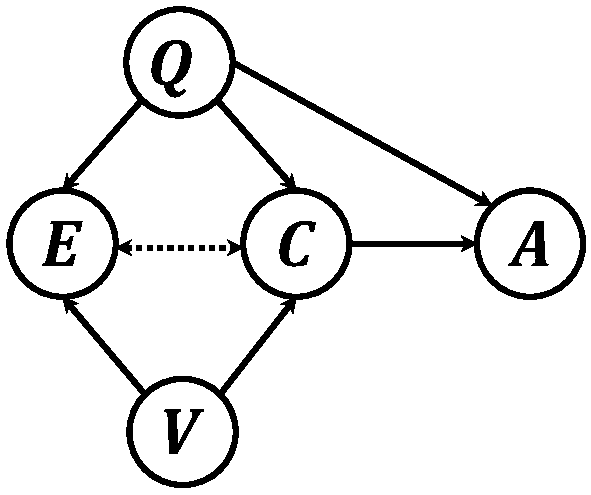
\includegraphics[scale=0.28]{fig/scm.pdf}
\caption{Causal Graph of VideoQA}
\vspace{-5pt}
\label{fig:scm}
\end{figure}

\section{Introduction}
\label{sec:introduction}


% 1.videoQA overview-----------------------------------------
In name of the interactive AI, Video Question Answering (VideoQA) \cite{fan2019heterogeneous} has relished a overwhelming expansion in various domains, such as vision-language navigation and communication systems. 
%
To answer the natural language question based on the video content, the task \textit{per se} has bred multi-modal nature in its process of reasoning, which demands thorough comprehension across visual content and linguistic semantics.

% %
% Aiming to answer the natural language question based on the video content, Video Question Answering (VideoQA) \cite{fan2019heterogeneous} 
% has witnessed aggressive expansion in various domains, such as vision-language navigation and communication systems.
% To make the task intriguing, the multi-modal nature of VideoQA has bred interactive AI in its reasoning, which demands thorough comprehension across visual scenes and linguistic semantics.
%
% In this regard, various VidoeQA model realizes their excellence via a common paradigm of two modules:
% (1) \textit{video-question encoder} encapsulates the video content and the question semantics to representations;
% and (2) \textit{answer decoder} exploits the multi-modal representations to model the vision-language interaction and generate an answer. 

\begin{figure}[t]
\centering
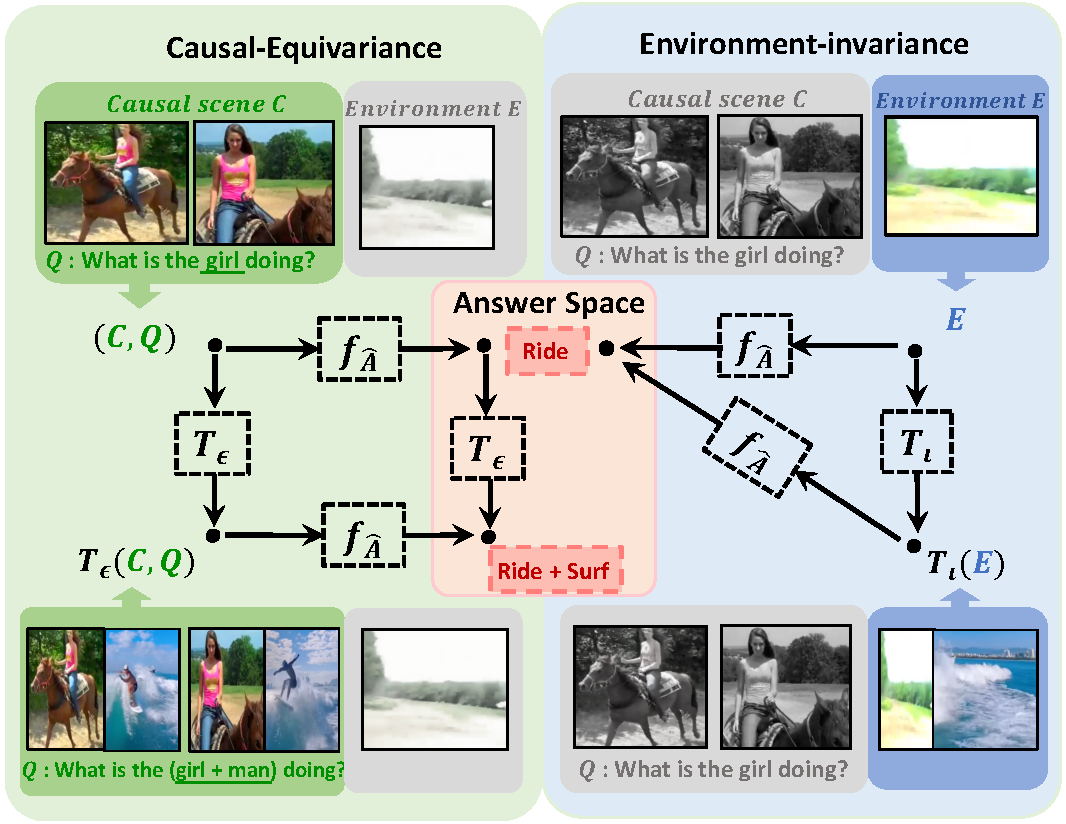
\includegraphics[scale=0.53]{fig/f1.pdf}
\caption{Illustration of causal-equivariant and environment-invariant principle, where $x$ is the model input, $f$ is a map from input space to answer space, $T$ is a transformation operator that applies to both input and answer space}.
% (\textcolor[rgb]{0,0.5,0}{Green}: causal-equivarince; \textcolor[rgb]{0.03,0.27,0.49}{Navy}: complement-invariance)}
\vspace{-5pt}
\label{fig:overview}
\end{figure}

% 2.problem of interpretable-------------------------------
Albeit the sterling performance, existing efforts usually express their reasoning mechanisms as black boxes. Unfortunately, peeping through their output does not reveal how machine leverage the multi-modal information, which refrains human intuition from machine intelligence and repels the nature of interactive AI. 
%the explanation of black-box models can provide insights into the relationship between input and output, thereby improving model design.
%shed light on model design
Worse still, overwhelming computational power has provoked the model complexity with billions of parameters, which, as a seed of distrust, shadowed the model's transparency along with our faith. 
%
Despite the necessity, the explainability of the current design still dwells on post-hoc visualization \cite{gao2018motionappearance,DBLP:conf/iccv/Liu0WL21,10.1145/3474085.3475620}, which is fragile against input perturbations, and less instructive to the predictive mechanism. 
%
% Clearly, inferring a reliable answer requires grounding rationale of the prediction, \ieto answer the million dollar question "which part of the video scene should be look at to answer the question". 
%
To the best of our knowledge, a self-interpretable VideoQA explainer that reveals the intrinsic prediction mechanism is critical to trustworthy videoQA but until-now lacking. 

% 3.partition the video to get interpretation ------------
Clearly, inferring a reliable answer requires a grounding rationale of the prediction, \ie to answer the million-dollar question "which part of the video scene should  be looking at?". 
%
Inspired by the information bottleneck, which tends to reduce the overload of information processing \cite{DBLP:conf/iclr/SaxeBDAKTC18}, we aim to find a shortcode for input video that preserves the maximum visual information toward the question, whose discovery will justify the prediction and increase the generalization. 
%
% Intuitively, filtering out task-irrelevant information reduces the overload of information processing, which naturally makes the representation more controllable.
%
Following this essence, one straightforward solution is to empower the model with discernment that splits the visual scene into two segments: 
(1) \textbf{causal scene} that retains the question-critical video content and preserving all the relevant information about the target answer, which naturally serves as interpretation for the prediction; (2) \textbf{environment scene} that holds answer-irrelevant environmental information of input video. 

% 4.euiqvariant and invariant for robust interpretation ---------------------------
% Modifying model's sensitivity to a certain transformation can have a substantial effect on the robustness of representation \cite{DBLP:journals/corr/abs-2111-00899}.
% %
% On top of the partition, one natural notion to acquire robust interpretation is making model sensitive to transformation of casual sense, while insensitive to transformation of complement sense.
% %
% Such philosophy of sensitivity is captured by the mathematical concept of equivariance and invariance: for a input$x$ and non-parametric transformation $T$, a encoder $f(.)$ is equivariant to $T$, if $∀x : f(T(x)) = T(f(x))$ ; Likewise, invariance is defined as $∀x : f(T(x)) = f(x)$.
% Specifically, the discovery of stable rationale implies two requirements on the partition:

%%%%%%
% Discovering  causal scene and answer is a luxury for videoQA without fine-grained supervision. 
Discovering causal scene without fine-grained supervision is a luxury for videoQA. Gazed upon the reasoning process, we argue crux of this problem is to amplify the connection between the causal scene and answer, while blocking the effect of environment. Following this line, we put forward \textit{Equivariance} and \textit{Invariance} principles to guide the partition learning.
% we borrow the mathematical concept of equivariance and invariance.
As shown in Figure \ref{fig:overview}, equivariance extends the model's sensitivity towards the a transformation $T$ on input $x$. Invariance, quite the contrary, inhibits the sensitivity and block model from input transformation. In light of this, the discovery of a stable rationale implies two requirements on the partition:
%
\begin{itemize}[leftmargin=*]
    \item \textbf{Causal-euqivariance.} In essence, transformation on the causal scene should cause the parallel change on the representation manifold. By introspecting ``How would the predictive answer vary if the causal scenes change?'', the grounding mechanism is aware of the transformations and thus maintains the predictive interpretation.
    In Figure \ref{fig:overview}, the euqivariance is exemplified in way that applying transformation $T$ to answer-critic information (\ie causal scene and question) should set off equivariant semantic change in answer space.
    In turn, a cautious formulation of such co-variation should helps the model to pinpoint the 'girl-on-horse' scene as grounding rationale for ``ride''.
    
    \item \textbf{Environmental-invariance.} On ground of the prophet, the answer prediction is invariant against permutation on environment scene, as it does not contribute to the reasoning mechanism or interpretation. 
    Consider the example in Figure \ref{fig:overview} again, since complement as ``landscape'' provide no evidence toward answer ``ride'', its corresponding transformation should reflect a homogeneity in the answer space. The invariance principle epitomizes such assumption by ruling a transformation that is in-vary to answer permutation.
\end{itemize}


%5.overall idea ------------------------------------------------------------------
Aspiring to capture grounding rationale, we formalize a model-agnostic learning framework, Equivariant and Invariant Grounding for Interpretable VideoQA (EGV), 
%
by asking the question ``what and how transformation should the model be equivariant or invariant to?'' 
%
Different from the previous effort that design supervised proxy task for geometric transformation \cite{DBLP:conf/iccv/ChengSM21}, 
% we adopted philosophy of causal intervention and design a saliency-aware temporal mix method for the video input, and impose 
we answer the ``what'' question by adopting the philosophy of causality \cite{pearl2009causal} and configure transformation as causal intervention operation that imposes scene-aware mixup \cite{DBLP:conf/iclr/ZhangCDL18} on the multi-modal input.
%
As for the question of how, we present a unified view of equivariant and invariant principles via the lens of temporal self-supervised learning, where the contrastive counterparts are bred through a disruption on the causal scene, environmental scene as well as vision-language alignment.

% where the contrastive counterparts are bred through a disruption on the causal and environmental scene, respectively.

% implemetation -----------------------------------------------------
In light of this idea, EGV absorbs three modules in addition to the backbone VideoQA model: a grounding indicator, an intervener, and a disruptor. 
%
In particular, the grounding indicator learns to separate the causal scenes as the interpretation and leave the rest as complement. Then the intervener performs a convex combination of two data points with different ratios on their causal and environmental parts. 
%
Noticeably, since mixing environment does not affect the reasoning dynamics, the answer is modified with the same ratio as the causal scene but independent to environmental one. 
%
By capturing the equivariance from the answer to the causal scene and the invariance to environment, the model perceives a faithful interpretation that preserves the predictive mechanism.
%
On top of the intervened video, the disruptor substitutes the complement scene with the stratification sampled from a memory bank (a collection of other training videos) and constitutes the “counterfactual video” as the positive sample.
Likewise, the negative sample is constructed via replacement on the causal scene. 
%
In addition to the visual negatives that ``disrupt'' the causal scene, the disruptor also develops alternatives by disrupting the visual-question coupling, to fortify their pair-wise cohesiveness.
% 
After acquiring anchor representation alongside its contrastive twins, the auxiliary contrastive objective reveals the discriminative representation purely from the scene of interest, thus fostering the robustness of interpretation.

Briefly put, our contributions are: 
\begin{itemize}[leftmargin=*]
    \item We proposed EGV, a model-agnostic VideoQA explainer that captures the intrinsic causal pattern in a self-interpretable manner.
    
    \item We investigate the soundness of grounding rationale by posing the equivariant-invariant principle on visual grounding and realize it via the causal instrument.
    
    \item We justify the superiority of EGV on three popular benchmark datasets (\ie MSVD-QA \cite{DBLP:conf/mm/XuZX0Z0Z17}, MSRVTT-QA \cite{DBLP:conf/mm/XuZX0Z0Z17},  NExT-QA \cite{DBLP:conf/cvpr/XiaoSYC21}) with extensive experiments, where our design outmatches all the state-of-the-art models.
\end{itemize}














